%!TEX TS-program = pdflatex
%!TEX encoding = UTF-8 Unicode

\documentclass[11pt, twoside, fleqn]{book}

%\flushbottom declaration makes all text pages the same height, adding extra vertical space when necessary to fill out the page.
\flushbottom

%The \raggedbottom declaration makes all pages the height of the text on that page. No extra vertical space is added.

% Allow an excess of 2.0pt per line
\hfuzz=2.0pt

% preamble should include, in this order:
\usepackage[T1]{fontenc}
% load babel here
\usepackage[english]{babel}
\usepackage[p,osf,swashQ,sups]{cochineal}
\usepackage[varqu,varl,var0]{inconsolata}
\usepackage[scale=.95,type1]{cabin}
\usepackage[cochineal,vvarbb,slantedGreek]{newtxmath}
% Other possibilities for slanted greeks https://ctan.math.ca/tex-archive/fonts/newtx/doc/newtxdoc.pdf
\usepackage[cal=boondoxo]{mathalfa}
\usepackage{amsmath}
%\usepackage{amssymb}
\numberwithin{equation}{chapter}
%\usepackage{mathrsfs}   %%%%% use \mathcal instead
\usepackage{anyfontsize}
\usepackage{chemfig}

\usepackage{xcolor}
\definecolor{brownfigs}{rgb}{0.7607843137254902,0.5607843137254902,0.2823529411764706}
\definecolor{bluefigs}{rgb}{0.2392156862745098,0.403921568627451,0.4823529411764706}
\definecolor{greyfigs}{rgb}{0.6509803921568627,0.6549019607843137,0.6392156862745098}

\let\oldvec=\vec % \oldvec tiene la flecha
\renewcommand{\vec}[1]{\boldsymbol{#1}}
%\renewcommand{\sen}[1]{\mathrm{sen\,#1}}
\newcommand{\vecuni}[1]{\hat{\boldsymbol{e}}_{#1}}
\newcommand{\hatvec}[1]{\hat{\boldsymbol{#1}}}
\newcommand{\final}{\text{final}}
\newcommand{\inicial}{\text{inicial}}
\newcommand{\fig}[1]{Figure \ref{fig:#1}}
\newcommand{\eqn}[1]{Eq.~\eqref{eq:#1}}
\newcommand{\vecdot}[2]{\boldsymbol{#1\!\cdot\!#2}}
\newcommand{\vecdotind}[4]{\boldsymbol{#1}_{#2}\boldsymbol{\cdot}\boldsymbol{#3}_{#4}}
\newcommand{\vecunidot}[2]{\hat{\boldsymbol{e}}_{#1}\!\boldsymbol{\cdot}\!\hat{\boldsymbol{e}}_{#2}}
\newcommand{\vectordotunit}[2]{\vec{#1}\!\boldsymbol{\cdot}\!\hat{\boldsymbol{e}}_{#2}}
\newcommand{\unitdotvector}[2]{\hat{\boldsymbol{e}}_{#1}\!\boldsymbol{\cdot}\!\vec{#2}}
\newcommand{\vecprod}[2]{\boldsymbol{#1}\times\boldsymbol{#2}}
\newcommand{\vecprodind}[4]{\boldsymbol{#1}_{#2}\times\boldsymbol{#3}_{#4}}
\newcommand{\vecuniprod}[2]{\hat{\boldsymbol{e}}_{#1}\times\hat{\boldsymbol{e}}_{#2}}
\newcommand{\vecmix}[3]{\boldsymbol{#1}\!\boldsymbol{\cdot}\!(\boldsymbol{#2}\times\boldsymbol{#3})}
\newcommand{\ie}{\textit{i.e.}}
\newcommand{\upd}{\mathrm{d}}
\newcommand{\deriv}[1]{\upd#1}
\newcommand{\derivp}[1]{\upd'\!#1}
\newcommand{\Deltap}[1]{\Delta'\!#1}
\newcommand{\diffin}[2]{\upd#1/\upd#2}
\newcommand{\diff}[2]{\dfrac{\upd#1}{\upd#2}}
\newcommand{\diffsec}[2]{\dfrac{\upd^2#1}{\upd#2^2}}
\newcommand{\diffn}[3]{\dfrac{\upd^{#3}#1}{\upd#2^{#3}}}
\newcommand{\diffnin}[3]{\upd^{#3}#1/\upd#2^{#3}}
\newcommand{\diffinpartial}[2]{\uppartial#1/\uppartial#2}
\newcommand{\diffpartial}[2]{\dfrac{\uppartial#1}{\uppartial#2}}
\newcommand{\diffsecpartial}[2]{\dfrac{\uppartial^2#1}{\uppartial#2^2}}
\newcommand{\mr}{m_{\text{r}}}
\newcommand{\diffnpartial}[3]{\dfrac{\uppartial^{#3}#1}{\uppartial#2^{#3}}}
\newcommand{\bra}[1]{\left.\left\langle #1 \right.\right|}
\newcommand{\ket}[1]{\left|\left\. #1 \right\rangle\right.}
\newcommand{\average}[1]{\left\langle #1 \right\rangle}
\newcommand{\absolute}[1]{\left| #1 \right|}
\newcommand{\enlevel}[3]{$#1\text{#2}_{#3}$}
\newcommand{\reynolds}{R\hspace{-1pt}e}
\newcommand{\amu}{m_{\text{un}}}
\newcommand{\amr}{A_{\text{r}}}
\newcommand{\mmr}{M_{\text{r}}}
\newcommand{\ab}[2]{#1_{\text{#2}}}
\newcommand{\abc}[3]{#1_{\text{#2}}^{\text{#3}}}
\newcommand{\parenthesis}[1]{\left(#1\right)}
\newcommand{\bracket}[1]{\left[#1\right]}
\newcommand{\bracet}[1]{\left\{#1\right\}}
\newcommand{\ccdot}{\vec{\cdot}}
\newcommand{\divop}[1]{\nabla\ccdot\,#1}
\newcommand{\curlop}[1]{\nabla\times#1}
\newcommand{\gradop}[1]{\nabla#1}
\newcommand{\diverg}[1]{\text{div~}#1}
\newcommand{\curl}[1]{\text{curl~}#1}
\newcommand{\grad}[1]{\text{grad~}#1}

\newcommand{\sect}[1]{Sec.~\ref{sec:#1}}
\newcommand{\app}[1]{Appendix.~\ref{sec:#1}}
\newcommand{\tab}[1]{Table~\ref{table:#1}}

\usepackage[a5paper]{geometry}
\geometry{textheight=17cm, textwidth=10.8cm, top=1.5cm, left=1.6cm, right=0.9cm, bottom=1.0cm}

\usepackage{booktabs}
\usepackage{threeparttable}
\usepackage{multirow}
%\usepackage{multicol}
\usepackage[version=4]{mhchem}

\usepackage{tikz-cd}
\usepackage{graphicx}
\usepackage{subcaption}
\usepackage[group-separator = {,}, input-protect-tokens]{siunitx}
\DeclareSIUnit\kgf{kgf}
\DeclareSIUnit\calorie{cal}
\DeclareSIUnit\atm{atm}
\DeclareSIUnit\gf{gf}
\DeclareSIUnit\dyne{dyn}
\DeclareSIUnit\erg{erg}
\DeclareSIUnit\hp{hp}
\DeclareSIUnit\poise{P}
\DeclareSIUnit\faraday{F}
\newcommand{\cgse}[1]{\text{~cgse$_{#1}$}}

\usepackage{nicefrac}
\usepackage{soul}

\usepackage{etoolbox}
% Make fancyhdr chapter first page
\patchcmd{\chapter}{\thispagestyle{plain}}{\thispagestyle{fancy}}{}{}

\usepackage{fancyhdr}
\fancyhead{} % clear all header fields
\fancyfoot{}
\renewcommand{\headrulewidth}{0pt}
%\fancyhead[LE]{\thepage\quad\nouppercase\leftmark}
%\fancyhead[LE]{\thepage\quad\sc\leftmark}
\fancyhead[LE]{\color{black!70}\small\sffamily\thepage}
\fancyhead[RE]{\color{black!70}\small\sffamily\rightmark}
%\fancyhead[RO]{\rightmark\quad\thepage}
\fancyhead[RO]{\color{black!70}\small\sffamily\thepage}
\fancyhead[LO]{\color{black!70}\small\sffamily\leftmark}
\pagestyle{fancy}
\renewcommand{\chaptermark}[1]{\markboth{\ #1}{}}
%\renewcommand{\sectionmark}[1]{\markright{\thesection.\ #1}}
\renewcommand{\sectionmark}[1]{\markright{#1}{}}

% Resetea el figure numbering para cada seccion
%\renewcommand{\thefigure}{\arabic{section}.\arabic{figure}}
\usepackage{chngcntr}
\counterwithin{figure}{chapter}
\counterwithout{section}{chapter}

\renewcommand\thesection{\S~\arabic{section}}
%\renewcommand\thechapter{\Roman{chapter}}
%\renewcommand\thepart{\Alph{part}}

\usepackage{titlesec}

\titleformat{\chapter}[display]
%{\sffamily\huge\color{black!70}\bfseries}
{\huge\color{black!70}\bfseries}
%{\MakeUppercase{\chaptertitlename}\ \thechapter}{10pt}{}
{\chaptertitlename\ \thechapter}{10pt}{}

\titleformat{\section}
%  {\normalfont\sffamily\large\color{black!80}}
{\normalfont\sffamily\bfseries\color{black!70}}{}{0pt} {\thesection.~}
%\setlength{\parskip}{0.5\baselineskip}

\usepackage[titles]{tocloft}
% Vertical space between entries in TOC
\renewcommand{\cftchapafterpnum}{\vskip-3pt}
\renewcommand{\cftsecafterpnum}{\vskip-3pt}
% Font changes to ToC content of sectional units
\renewcommand{\cftpartfont}{\normalfont\bfseries}% \part font in ToC
\renewcommand{\cftchapfont}{\small\bfseries} % \chapter font in ToC
\renewcommand{\cftsecfont}{\small} % \section font in ToC
% \renewcommand{\cftsubsecfont}{\normalfont\itshape}        % \subsection font in ToC
% \renewcommand{\cftsubsubsecfont}{\normalfont\small}       % \subsubsection font in ToC
% Remove dots in toc
\renewcommand{\cftdot}{}
% Include the Chapter X in tocs, the parts does not work as pointed out in tocloft
\newlength{\mylenprt}
\newlength{\mylenchp}
\renewcommand{\cftchappresnum}{\chaptername~}
% \renewcommand{\cftsecpresnum}{\sectionname~}
\renewcommand{\cftchapaftersnum}{.}
\renewcommand{\cftsecaftersnum}{.}
% \settowidth{\mylenprt}{\cftsecfont\cftsecpresnum\cftsecaftersnum}
\settowidth{\mylenchp}{\cftchapfont\cftchappresnum\cftchapaftersnum}
% \addtolength{\mylenprt}{\cftsecnumwidth}
\addtolength{\mylenchp}{\cftchapnumwidth}
\addtolength{\mylenprt}{-13pt}
\addtolength{\mylenchp}{-13pt}
% \setlength{\cftsecnumwidth}{\mylenprt}
\setlength{\cftchapnumwidth}{\mylenchp}

% Space between lines in pt
\renewcommand{\baselinestretch}{1.0}

\setlength{\parskip}{0pt}
\setcounter{secnumdepth}{1}

\usepackage{caption}
\usepackage[labelfont={color=black!80,footnotesize,bf,sf}, textfont={color=black!80,small}, figurename=Figure]{caption}

\usepackage[shortlabels]{enumitem}
\setlist{nosep}
% \setlength{\parskip}{1ex plus 0.5ex minus 0.2ex}
\setlength{\parskip}{0pt}

\usepackage[colorlinks=true]{hyperref}
\hypersetup{
  colorlinks,
  linkcolor=brownfigs,
  linktoc=all
}

% Suppresses page numbers and headings from appearing on empty pages
\usepackage{emptypage}
\usepackage{pdfpages}

\usepackage{dialogue}
\usepackage{lips}

% \title{Solid State Physics}
% % \author{I. V. Savelyev}
% % \date{2020}

\begin{document}

% Reduce spaces before and after equations
\setlength{\abovedisplayskip}{3pt}
\setlength{\belowdisplayskip}{3pt}
\setlength{\abovedisplayshortskip}{3pt}
\setlength{\belowdisplayshortskip}{3pt}

\frontmatter


\includepdf{figures/ssp_fc.pdf}
\cleardoublepage
% !TEX root = saveliev_physics_general_course_2.tex
%!TEX TS-program = pdflatex
%!TEX encoding = UTF-8 Unicode


%\cleardoublepage
\thispagestyle{empty}
%\maketitle
%\vspace*{1cm}
\noindent
\hspace{50pt}{\large\bfseries I. V. SAVELYEV}
\vspace{40pt}

\noindent
\hspace{50pt}{\Huge\bfseries PHYSICS}
\vspace{10pt}

\noindent
\hspace{50pt}{\Large\bfseries A GENERAL COURSE}
\vspace{10pt}

\noindent
\hspace{50pt}{\bfseries (In three volumes)}
\vspace{30pt}

\noindent
\hspace{120pt}{\Large\bfseries VOLUME~II}
\vspace{12pt}

\noindent
\hspace{120pt}{\huge ELECTRICITY}
\vspace{0.3cm}

\noindent
\hspace{120pt}{\huge AND MAGNETISM}
\vspace{0.5cm}

\noindent
\hspace{120pt}{\huge WAVES}
\vspace{0.5cm}

\noindent
\hspace{120pt}{\huge OPTICS}

\vspace*{3cm}
\hspace{120pt}
\includegraphics[width=0.1\textwidth]{figures/mirlogo.pdf}

\hspace{120pt}{\large MIR PUBLISHERS}

\hspace{120pt}{\large MOSCOW}

%\cleardoublepage
\clearpage

\noindent
Translated from Russian by G. Leib

\vspace{40pt}

%Versi\'on electr\'onica publicada en 2020 por\\[1pt]
%Leandro N. Acquaroli
\noindent
First published 1980

\noindent
Revised from the 1978 Russian edition

\noindent
Second printing 1985

\noindent
Third printing 1989

%\url{http://mirtitles.org}

%The project files are available at:

%\url{https://gitlab.com/mirtitles/pfe}

\vfill
\noindent
\textit{Printed in the Union of Soviet Socialist Republics}

\vspace{30pt}

\noindent
ISBN 5-03-000902-7, 1978

\noindent
ISBN 5-03-000900-0, 1980

\thispagestyle{empty}

\cleardoublepage
% !TEX root = epifanov_solid_state_physics.tex
%!TEX TS-program = pdflatex
%!TEX encoding = UTF-8 Unicode


\chapter*{PREFACE}
\addcontentsline{toc}{chapter}{Preface}
\chaptermark{PREFACE}

\vspace*{-12pt}

Ten years have passed since the first Russian edition of this textbook was published. In this time solid state physics has developed rapidly as the scientific background of numerous front-line branches of technology, absorbing new discoveries and theories. This has been considered in preparing the new edition.

At the same time college curricula have been changed to improve the basic preparation of versatile engineers, especially in physics and mathematics. This too had to be reflected in this book.

Also, the years that have elapsed since the first edition have seen much comment, some critical, and many proposals from Soviet and foreign readers---from college teachers and students, teachers of vocational and secondary schools, engineers and scientists. The author is grateful for all the comment and proposals.

There was a need therefore to revise the book completely. As in the first edition, the presentation of material has followed the aim of elucidating the physical nature of the phenomena discussed. But, where possible, the qualitative relations are also presented, often though without rigorous mathematics.

The manuscript was reviewed in detail by Prof. L. L. Dashkevich, Dr. of Technical Sciences, and Prof. I. G. Nekrashevich, Honored Scientist of the Belorussian Republic. It was perused by Prof. L. A. Gribov, Dr. of Mathematical and Physical Sciences, Assistant Prof. V. B. Zernov, and Z. S. Sazonova. The author extends sincere thanks for their efforts and criticism, which he took into account when revising the manuscript.

The author is also indebted to Senior Lecturer F. Zh. Vilf, Cand. of Technical Sciences, and Assistant Prof. Yu. A. Moma, Cand. of Technical Sciences, for manuals used in this textbook on superconductivity, Gunn effect, and principles of operation of impulse and high-frequency diodes, and to Z. I. Epifanova for all her work in preparing the manuscript.

The author will be most grateful for comment and proposals that might improve this book. They should be sent to the publishers.

\begin{flushright}
	\emph{G. I. E.}
\end{flushright}

%\pagestyle{mystyle}

\cleardoublepage
{\hypersetup{linkcolor=black!80}
	% or \hypersetup{linkcolor=black}, if the colorlinks=true option of hyperref is used
	\tableofcontents
}
\cleardoublepage

\mainmatter

% \cleardoublepage
% !TEX root = saveliev_physics_general_course_1.tex
%!TEX TS-program = pdflatex
%!TEX encoding = UTF-8 Unicode


\chapter{KINEMATICS}\label{chap:1}

\section{Mechanical motion}\label{sec:1_1}

Mechanical motion is the simplest form of motion of matter. It consists in the movement of bodies or their parts relative to one another. We can see movements of bodies everywhere in our ordinary life. This is why mechanical notions are so clear. This also explains the fact that mechanics was the first of all the natural sciences to be developed very broadly.

A combination of bodies separated for consideration is called a \textbf{mechanical system}. The bodies to be included in a system depend on the nature of the problem being solved. In a particular case, a system may consist of a single body.

It was indicated above that motion in mechanics is defined as the change in the mutual arrangement of bodies. If we imagine a separate isolated body in a space where no other bodies are present, then we cannot speak of the motion of the body because there is nothing with respect to which the body could change its position. It thus follows that if we intend to study the motion of a body, then we must indicate with respect to what other bodies the given motion occurs.

Motion occurs both in space and in time (space and time are inalienable forms of existence of matter). Consequently, to describe motion, we must also determine time. We use a timepiece (watch or clock) for this purpose.

A combination of bodies that are stationary relative to one another with respect to which motion is being considered and a timepiece indicating the time forms a \textbf{reference frame}.

The motion of the same body relative to different reference frames may have a different nature. For example, let us imagine a train gaining speed. Suppose that a passenger is walking with a constant velocity along the corridor of one of the cars of the train. The motion of the passenger relative to the ear will be uniform, and relative to the Earth's surface it will be accelerated.

To describe the motion of a body means to indicate for every moment of time the position of the body in space and its velocity. To set the state of a mechanical system, we must indicate the positions and the velocities of all the bodies forming the system. A typical problem of mechanics consists in determining the states of a system at all the following moments of time $t$ when we know the state of the system at a certain initial moment $t_0$ and also the laws governing the motion.

It must be noted that no physical problem can be solved absolutely exactly. An approximate solution is always obtained. The degree of approximation is determined by the nature of the problem and the object to be achieved. In solving a problem approximately, we disregard the factors that are not significant in the given case. For example, we may often disregard the dimensions of the body whose motion is being studied. For instance, it is quite possible to disregard the Earth's dimensions when treating its motion about the Sun. This allows us to considerably simplify our description of the motion because the Earth's position in space can be determined by a single point.

A body whose dimensions may be disregarded in the conditions of a given problem is called a \textbf{point particle} (or simply a \textbf{particle}). Whether or not we may consider a given body as a particle depends not on the dimensions of the body, but on the conditions of the problem. The same body in some cases may be treated as a particle, but in others it must be considered as an extended body.

When speaking about a body as a particle, we disengage ourselves from its dimensions. Another abstraction which we have to do with in mechanics is a perfectly rigid body. Absolutely undeformable bodies do not exist in nature. Any body deforms to a greater or smaller extent, \ie, changes its shape and dimensions, under the action of forces applied to it. The deformations of bodies when considering their movements may often be disregarded, however. If this is done, then the body is called perfectly rigid. Thus, a body whose deformations may be disregarded in the conditions of a given problem is called a \textbf{perfectly rigid}, or simply a \textbf{rigid body}.

Any motion of a rigid body can be resolved into two basic kinds of motion---\textbf{transla\-tional motion} and \textbf{circular motion}.

Translational motion (translation) is defined as motion in which any straight line associated with the moving body remains parallel to itself (\fig{1_1}).

In circular motion (rotation), all the points of a body move in circles whose centers are on a single straight line called the axis of rotation (\fig{1_2}). The axis of rotation can be outside a body (see \fig{1_2}b).

\begin{figure}[t]
	\begin{minipage}[t]{0.5\linewidth}
		\begin{center}
			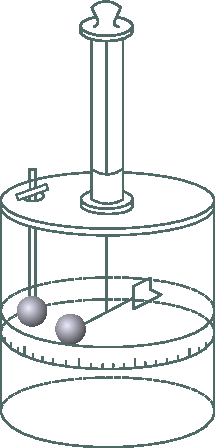
\includegraphics[scale=0.95]{figures/cap_01/fig_1_1.pdf}
			\caption[]{}
			\label{fig:1_1}
		\end{center}
	\end{minipage}
	\hfill{ }%\hspace{-0.1cm}
	\begin{minipage}[t]{0.5\linewidth}
		\begin{center}
			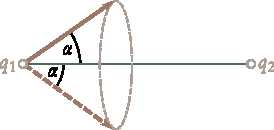
\includegraphics[scale=0.95]{figures/cap_01/fig_1_2.pdf}
			\caption[]{}
			\label{fig:1_2}
		\end{center}
	\end{minipage}
%\vspace{-0.5cm}
\end{figure}

\begin{figure}[t]
	\begin{center}
		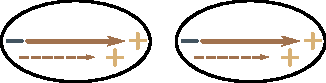
\includegraphics[scale=0.95]{figures/cap_01/fig_1_3.pdf}
		\caption[]{}
		\label{fig:1_3}
	\end{center}
	\vspace{-0.8cm}
\end{figure}

Since when treating a body as a particle we ignore its length, the concept of circular motion about an axis passing through such a body cannot be applied to it.

To acquire the possibility of describing motion quantitatively, we have to associate a \textbf{coordinate system} (for example a Cartesian one) with the bodies forming a reference frame. Hence, the position of a particle can be determined by setting the three numbers $x$, $y$, and $z$---the Cartesian coordinates of the particle. A coordinate system can be made by forming a rectangular lattice from identical rods or rules graduated to a definite scale: (\fig{1_3}). Identical clocks synchronized with one another must be placed at the lattice points. The position of a particle and the moment of time corresponding to this position are recorded on the graduated rods and the clock closest to the particle.

It is simpler to treat a point particle than an extended body. We shall therefore first study the mechanics of a particle, and then go over to the mechanics of a rigid body. We shall start with kinematics, and then delve into dynamics. We remind our reader that \textbf{kinematics} studies the motion of bodies without regard to what causes this motion. \textbf{Dynamics} studies the motion of bodies with a view to what causes this motion to have the nature it does, \ie, with a view to the interactions between bodies.

\section{Vectors}\label{sec:1_2}

\textbf{Definition of a Vector.} Vectors are defined as quantities characterized by a numerical value and a direction and also as ones that are added according to the triangle or parallelogram method\footnote{According to a stricter definition, a vector is a combination of three quantities that transform when the coordinate axes rotate according to a definite law.}. The last requirement is a very significant one. We can indicate quantities characterized by a numerical value and a sense of direction but that are added in a different way than vectors. We shall take as an example the rotation of a body about an axis through the finite angle $\varphi$. Such rotation can be depicted in the form of a segment of length $\varphi$ directed along the axis about which rotation is occurring and pointing in a direction associated with that of rotation according to the right-hand screw rule. The top portion of \fig{1_4} shows two consecutive turns of the sphere through the angles $\pi/2$ depicted by the segments $\varphi_1$ and $\varphi_2$. The first turn about axis $1$---$1$ transfers point $A$ of the sphere to position $A'$, and the second turn about axis $2$---$2$ transfers it to position $A''$. The same result, \ie, transfer of point $A$ to position $A''$, can be achieved by turning the sphere about axis $3$---$3$ (see the bottom portion of \fig{1_4}) through the angle $\pi$. Hence, such a turn should be considered as the sum of the turns <p1 and <p 2 • It cannot be obtained from the segments $\varphi_1$ and $\varphi_2$, however, by adding them according to the parallelogram method. Such addition gives a segment of length $\pi/\sqrt{2}$ instead of the required length $\pi$. Rotation through the angle $\pi/\sqrt{2}$ transfers point $A$ to point $A'''$. It thus follows that the turns through finite angles depicted by the directed segments do not have the properties of vectors.

\begin{figure}[t]
	\begin{center}
		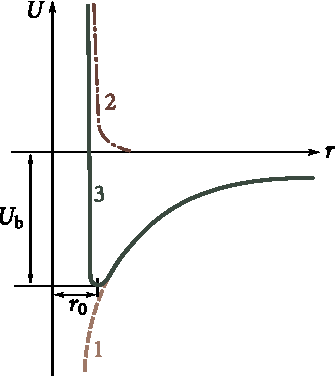
\includegraphics[scale=0.9]{figures/cap_01/fig_1_4.pdf}
		\caption[]{}
		\label{fig:1_4}
	\end{center}
\vspace{-0.8cm}
\end{figure}

The numerical value of a vector is called its magnitude. Figuratively speaking, the magnitude of a vector indicates its length. The magnitude of a vector is a scalar, and always a positive one.

Vectors are represented graphically by arrows. The length of an arrow determines to the established scale the magnitude of the relevant vector, and the arrow points in the direction of the vector.

Vectors are customarily distinguished by setting their symbols in boldface type, for example, $\vec{a}$, $\vec{b}$, $\vec{v}$ and $\vec{F}$. The same symbols set in italics signify the magnitude of the relevant vectors, for example, $a$ is the magnitude of the vector $\vec{a}$\footnote{In handwriting, vectors are denoted by arrows over their symbols (for example, $\oldvec{a}$. In this case, the same letter without the arrow stands for the magnitude of the vector.}. It is sometimes necessary to express the magnitude by placing a vertical bar (an absolute value sign) on each side of the symbol for the vector. Thus, $|a|$ is the magnitude of the vector $\vec{a}$. This representation is used, for example, to show the magnitude of the sum of the vectors $\vec{a}_1$ and $\vec{a}_2$:
\begin{equation}\label{eq:1_1}
	|\vec{a}_1 + \vec{a}_2| = \text{magnitude of the vector } (\vec{a}_1 + \vec{a}_2).
\end{equation}

\noindent
In this case, the notation $a_1+a_2$ signifies the sum of the magnitudes of the vectors being added, which in general does not equal the magnitude of the sum of the vectors (the two sums will be equal only when the vectors being added have the same direction).

Vectors directed along parallel straight lines (in the same or in opposite directions) are called \textbf{collinear}. Vectors in parallel planes are called \textbf{coplanar}. Collinear vectors can be arranged along the same straight line and coplanar vectors can be brought into one plane by parallel translation.

Collinear vectors equal in magnitude and having the same direction are considered to equal each other\footnote{What is meant are the so-called \textbf{free vectors}, \ie, vectors that can be drawn from any point in space. Also distinguished are \textbf{slip vectors} whose tail can be placed at any point on the straight line along which the vector is directed, and localized vectors, which are applied to a definite point. The last two kinds of vectors can be expressed through free vectors. This is why vector calculus is based on the concept of the free vector, usually called simply a vector.}.

\textbf{Vector Addition and Subtraction.} It is more convenient to add vectors in practice without constructing a parallelogram. Examination of \fig{1_5} shows that we can achieve the same result if we bring the tail of the second vector in contact with the tip of the first one, and then draw the resultant vector from the tail of the first vector to the tip of the second one. It is very good to use this procedure when we have to add more than two vectors (\fig{1_6}).

\begin{figure}[t]
	\begin{minipage}[t]{0.5\linewidth}
		\begin{center}
			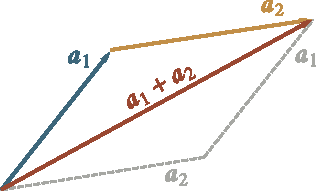
\includegraphics[scale=0.95]{figures/cap_01/fig_1_5.pdf}
			\caption[]{}
			\label{fig:1_5}
		\end{center}
	\end{minipage}
	\hfill{ }%\hspace{-0.1cm}
	\begin{minipage}[t]{0.5\linewidth}
		\begin{center}
			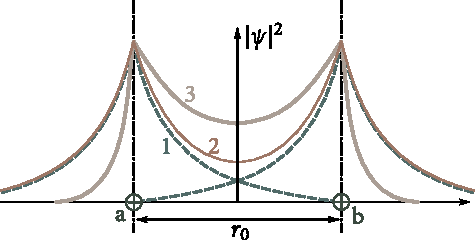
\includegraphics[scale=0.95]{figures/cap_01/fig_1_6.pdf}
			\caption[]{}
			\label{fig:1_6}
		\end{center}
	\end{minipage}
\vspace{-0.7cm}
\end{figure}

The difference of two vectors $\vec{a}$ and $\vec{b}$ is defined as such a vector $\vec{c}$ which when added to the vector $\vec{b}$ gives the vector $\vec{a}$ (\fig{1_7}---the vector $-\vec{b}$ depicted by a dash line will be treated below The magnitude of the difference of two vectors, like the magnitude of a sum [see \eqn{1_1}], may be written only with the aid of vertical bars:
\begin{equation}\label{eq:1_2}
|\vec{a}_1 - \vec{a}_2| = \text{magnitude of the vector } (\vec{a}_1 - \vec{a}_2),
\end{equation}

\noindent
because the notation $a_1-a_2$ signifies the difference of the magnitudes of the vectors $\vec{a}_1$ and $\vec{a}_2$, which, generally speaking, does not equal the magnitude of the vector difference.

\textbf{Multiplication of a Vector by a Scalar.} Multiplication of the vector $\vec{a}$ by the scalar $\alpha$ yields a new vector $\vec{b}=\alpha\,\vec{a}$ whose magnitude is $|\alpha|$ times that of the vector a (\ie, $b=|\alpha|a$). The direction of the vector $\vec{b}$ either coincides with that of the vector $\vec{a}$ (if $\alpha>0$), or is opposite to it (if $\alpha<0$). It follows from the above that multiplication by $-1$ reverses the direction of a vector. Consequently, the vectors $\vec{a}$ and $-\vec{a}$ have the same magnitudes, but are opposite in direction. It is simple to see with the aid of  \fig{1_7} that subtraction of the vector $\vec{b}$ from the vector $\vec{a}$ is equivalent to addition of the vector $-\vec{b}$ to the vector $\vec{a}$.

It follows from our definition of multiplication of a vector by a scalar that any vector $\vec{a}$ can be represented in the form
\begin{equation}\label{eq:1_3}
\vec{a} = a\,\vecuni{a},
\end{equation} 

\noindent
where $a$ is the magnitude of the vector $\vec{a}$ and $\vecuni{a}$, is vector with a magnitude of unity and of the same direction as $\vec{a}$ (\fig{1_8}).

The vector $\vecuni{a}$ is called the unit vector of the vector $\vec{a}$. The unit vector can be represented in the form
\begin{equation}\label{eq:1_4}
\vecuni{a} = \frac{\vec{a}}{a},
\end{equation}

\noindent
whence it follows that it is a dimensionless quantity.

\begin{figure}[t]
	\begin{minipage}[t]{0.5\linewidth}
		\begin{center}
			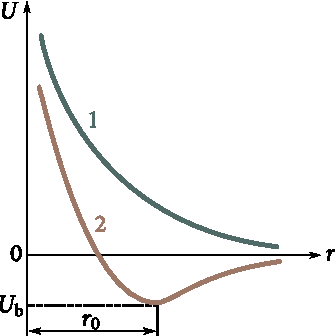
\includegraphics[scale=0.9]{figures/cap_01/fig_1_7.pdf}
			\caption[]{}
			\label{fig:1_7}
		\end{center}
	\end{minipage}
	\hfill{ }%\hspace{-0.1cm}
	\begin{minipage}[t]{0.5\linewidth}
		\begin{center}
			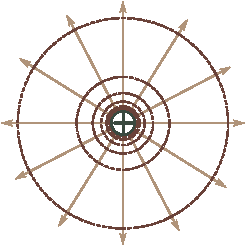
\includegraphics[scale=0.95]{figures/cap_01/fig_1_8.pdf}
			\caption[]{}
			\label{fig:1_8}
		\end{center}
	\end{minipage}
\vspace{-0.6cm}
\end{figure}

Unit vectors can be compared not only with vectors, but also with any direction in space. For example, $\vecuni{x}$ is the unit vector of the coordinate axis $x$, $\vecuni{n}$ is the unit vector of a normal to a curve or surface, and $\vecuni{\tau}$ is the unit vector of a tangent to a curve.

\textbf{Linear Relation Between Vectors.} Let us consider three non-collinear vectors $\vec{a}$, $\vec{b}$ and $\vec{c}$ that are in one plane. A glance at \fig{1_9} shows that any of them (for instance, $\vec{c}$) can be expressed through the other two with the aid of the relation
\begin{equation}\label{eq:1_5}
\vec{c} = \alpha\vec{a} + \beta\vec{b},
\end{equation}

\noindent
where $\alpha$ and $\beta$ are scalars (for the case shown in the figure, $\alpha>1$ and $-1<\beta<0$). Hence, we conclude that any vector $\vec{c}$ that is in the same plane as the non-collinear vectors $\vec{a}$ and $\vec{b}$ can be expressed through the latter with the aid of linear relation~\eqref{eq:1_5}. When the vectors $\vec{a}$ and $\vec{b}$ are fixed, any third vector is unambiguously determined by the two quantities $\alpha$ and $\beta$.

Assume that we have three vectors $\vec{a}$, $\vec{b}$ and $\vec{c}$, each of which is not coplanar with the other two.\footnote{Two vectors are always coplanar. This follows from the fact that their tails can he made to coincide by translation, and they will thus be in one plane.} By analogy with \eqn{1_5}, we can see quite easily that any vector $\vec{d}$ can be represented as a linear combination of the given vectors:
\begin{equation}\label{eq:1_6}
\vec{d} = \alpha\vec{a} + \beta\vec{b} + \gamma\vec{c},
\end{equation}

\noindent
When the vectors $\vec{a}$, $\vec{b}$ and $\vec{c}$ are fixed, any vector $\vec{d}$ is unambiguously determined by the three quantities $\alpha$, $\beta$ and $\gamma$, each of which may be either positive or negative.

\textbf{Projection of a Vector.} Let us consider a direction in space that we shall set by the axis $l$ (\fig{1_10}). Let the vector $\vec{a}$ make the angle $\varphi$ with the axis $l$\footnote{If the straight line along which the vector $\vec{a}$ is directed and the axis $l$ do not intersect, the angle $\varphi$ should be found by drawing a straight line parallel to the vector $\vec{a}$ and intersecting the axis $l$. The angle between this line and the axis $l$ will be the angle $\varphi$ we are interested in.}. The quantity
\begin{equation}\label{eq:1_7}
a_l = a\, \cos\varphi
\end{equation}

\noindent
(where $a$ is the magnitude of the vector) is called the projection of the vector $\vec{a}$ onto the axis$l$. A projection is designated by the same symbol as its vector, with the addition of a subscript showing the direction onto which the vector has been projected. 

\begin{figure}[t]
	\begin{minipage}[t]{0.5\linewidth}
		\begin{center}
			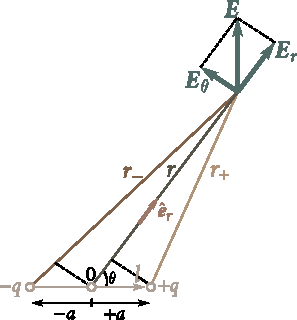
\includegraphics[scale=1]{figures/cap_01/fig_1_9.pdf}
			\caption[]{}
			\label{fig:1_9}
		\end{center}
	\end{minipage}
	\hfill{ }%\hspace{-0.1cm}
	\begin{minipage}[t]{0.5\linewidth}
		\begin{center}
			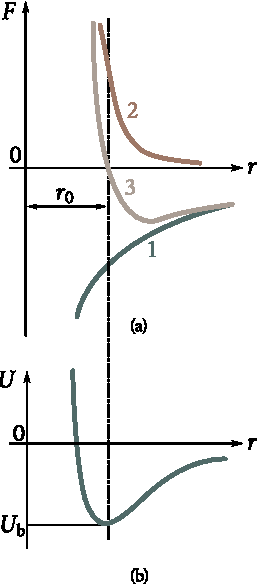
\includegraphics[scale=0.95]{figures/cap_01/fig_1_10.pdf}
			\caption[]{}
			\label{fig:1_10}
		\end{center}
	\end{minipage}
	\vspace{-0.7cm}
\end{figure}

A projection of a vector is an algebraic quantity. If the vector makes an acute angle with the given direction, then $\cos\varphi>0$, and the projection is positive. If the angle $\varphi$ is obtuse, then $\cos\varphi<0$, and, consequently, the projection is negative. When a vector is at right angles to a given axis, its projection equals zero.

The projection of a vector has a simple geometrical meaning. It equals the distance between the projections of the tail and the tip of the segment depicting the given vector onto the given axis. When $\varphi<\pi/2$, this distance is assumed to be positive, and when $\varphi>\pi/2$, it is negative.

Let $\vec{a} = \vec{a}_1+\vec{a}_2+\vec{a}_3+\vec{a}_4$ (\fig{1_11}). It is easy to see from the figure that the projection of the resultant vector a onto a direction $l$ equals the sum of the projections of the separate vectors being added:
\begin{equation}\label{eq:1_8}
a_l = a_{1l}+a_{2l}+a_{3l}+a_{4l}.
\end{equation}

\noindent
We must remind our reader that when adding the projections of the vectors shown in \fig{1_11}, the distances $0$---$1$, $1$---$2$, and $2$---$3$ have to be taken with the plus sign, and the distance $3$---$4$ with the minus sign. Equation~\eqref{eq:1_8} holds for any number of addends.

\textbf{Expressing a Vector Through Its Projections onto the Coordinate Axes.} Let us take Cartesian coordinate axes and consider the vector $\vec{a}$ in a plane at right angles to the $z$-axis (\fig{1_12}). We shall introduce the unit vectors of the coordinate axes, \ie, the unit vectors $\vecuni{x}$, $\vecuni{y}$ and $\vecuni{z}$ ($\vecuni{z}$ is not shown in the drawing, it is perpendicular to the plane of the drawing and directed toward us). It must be noted that these three unit vectors completely determine a system of coordinates and are therefore called the \textbf{basis of the coordinate system}.

\begin{figure}[t]
	\begin{minipage}[t]{0.5\linewidth}
		\begin{center}
			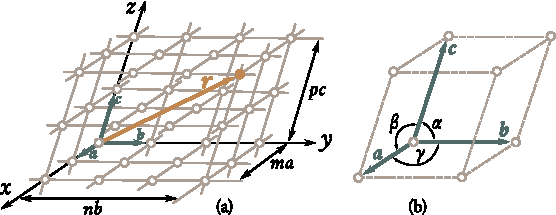
\includegraphics[scale=1]{figures/cap_01/fig_1_11.pdf}
			\caption[]{}
			\label{fig:1_11}
		\end{center}
	\end{minipage}
	\hfill{ }%\hspace{-0.1cm}
	\begin{minipage}[t]{0.5\linewidth}
		\begin{center}
			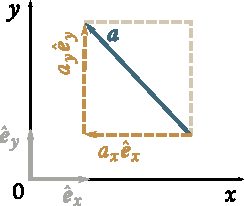
\includegraphics[scale=0.95]{figures/cap_01/fig_1_12.pdf}
			\caption[]{}
			\label{fig:1_12}
		\end{center}
	\end{minipage}
	\vspace{-0.8cm}
\end{figure}

Inspection of \fig{1_12} shows that the vector $\vec{a}$ can be represented in the form of a linear combination of the unit vectors $\vecuni{x}$ and $\vecuni{y}$ [see \eqn{1_5}]:
\begin{equation*}
\vec{a} = a_x \vecuni{x} + a_y \vecuni{y}.
\end{equation*}

\noindent
The projections of the vector onto the coordinate axes play the part of the coefficients $\alpha$ and $\beta$. In the example being considered, the projection $a_x$ is negative, therefore the vector $a_x\vecuni{x}$ has a direction opposite to that of the unit vector $\vecuni{x}$.

We took the vector $\vec{a}$ perpendicular to the $z$-axis owing to which $a_z=0$. In the general case when all three projections of a vector differ from zero, we have
\begin{equation}\label{eq:1_9}
\vec{a} = a_x \vecuni{x} + a_y \vecuni{y} + a_z \vecuni{z},
\end{equation}

\noindent
Thus, any vector can be expressed through its projections onto the coordinate axes and the unit vectors of these axes. Therefore, the projections of a vector onto the coordinate axes are called its \textbf{components}.

The components $a_x$, $a_y$, $a_z$ equal (with an accuracy to the sign) the sides of a right parallelepiped in which the vector $\vec{a}$ is the major diagonal (\fig{1_13}). We therefore have
\begin{equation}\label{eq:1_10}
a^2 = a_x^2 + a_y^2 + a_z^2.
\end{equation}

Assume that $\vec{c}=\vec{a}+\vec{b}$. Representing each of these vectors in accordance with \eqn{1_9}, we get
\begin{equation*}
c_x\vecuni{x} + c_y\vecuni{y} + a_z\vecuni{z} = (a_x+b_x)\vecuni{x} + (a_y+b_y)\vecuni{y} + (a_z+b_z)\vecuni{z}
\end{equation*}

\noindent
(we have factored out $\vecuni{x}$, $\vecuni{y}$, and $\vecuni{z}$)· Equal vectors have identical projections onto the coordinate axes. On these grounds, we can write that
\begin{equation}\label{eq:1_11}
c_x=a_x+b_x,\quad c_y=a_y+b_y,\quad a_z=a_z+b_z
\end{equation}

\noindent
[compare with \eqn{1_8}]. Equations~\eqref{eq:1_11} express analytically the rule of vector addition. They hold for any number of addends.

\textbf{Position Vector.} The position vector (or radius vector) $\vec{r}$ of a point is defined as the vector drawn from the origin of coordinates to the given point (\fig{1_14}). Its projections onto the coordinate axes equal the Cartesian coordinates of the given point:
\begin{equation}\label{eq:1_12}
r_x=x,\quad r_y=y,\quad r_z=z.
\end{equation}

\noindent
Consequently, in accordance with \eqn{1_9}, the position vector can be represented in the form
\begin{equation}\label{eq:1_13}
\vec{r} = x\vecuni{x} + y\vecuni{y} + z\vecuni{z}.
\end{equation}

\noindent
By \eqn{1_10}, we have
\begin{equation}\label{eq:1_14}
r^2 = x^2 + y^2 + z^2.
\end{equation}

\begin{figure}[t]
	\begin{minipage}[t]{0.5\linewidth}
		\begin{center}
			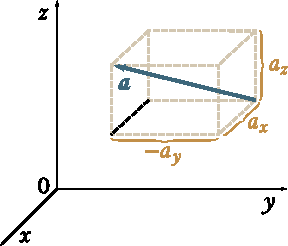
\includegraphics[scale=1]{figures/cap_01/fig_1_13.pdf}
			\caption[]{}
			\label{fig:1_13}
		\end{center}
	\end{minipage}
	\hfill{ }%\hspace{-0.1cm}
	\begin{minipage}[t]{0.5\linewidth}
		\begin{center}
			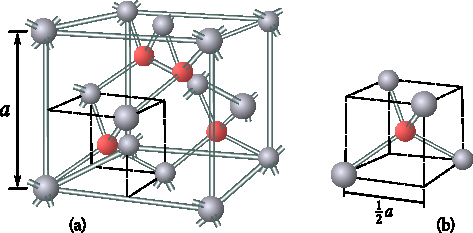
\includegraphics[scale=0.95]{figures/cap_01/fig_1_14.pdf}
			\caption[]{}
			\label{fig:1_14}
		\end{center}
	\end{minipage}
\vspace{-0.3cm}
\end{figure}

\begin{figure}[t]
	\begin{center}
		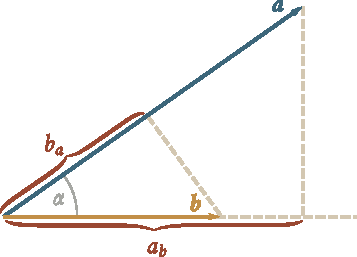
\includegraphics[scale=0.95]{figures/cap_01/fig_1_15.pdf}
		\caption[]{}
		\label{fig:1_15}
	\end{center}
	\vspace{-1.0cm}
\end{figure}

\textbf{The Scalar Product of Vectors.} Two vectors $\vec{a}$ and $\vec{b}$ can be multiplied by each other in two ways. One of them results in a scalar quantity, and the other in a certain new vector. Accordingly, two products of vectors are distinguished---the scalar product and the vector product. It must be noted that \textit{the operation of dividing a vector by a vector does not exist}.

The scalar product of the vectors $\vec{a}$ and $\vec{b}$ is defined as the scalar quantity equal to the product of the magnitudes of these vectors and the cosine of the angle $\alpha$ between them:
\begin{equation}\label{eq:1_15}
\vecdot{a}{b} = ab\sin\alpha
\end{equation}

\noindent
(\fig{1_15}). When writing a scalar product, the symbols of the vectors being multiplied are usually written next to each other with dot between them (this is why a scalar product is also called a dot product; sometimes nothing is used between the symbols)\footnote{The dot symbol between vectors is preferred in the \LaTeX version to adopt a more modern approach.}. Equation~\eqref{eq:1_15} expresses an algebraic quantity: when $\alpha$ is acute, we have $\vecdot{a}{b}>0$, and when it is obtuse, we have $\vecdot{a}{b}<0$. The scalar product of mutually perpendicular vectors ($\alpha=\pi/2$) equals zero.

It must be noted that by the square of a vector is always meant the scalar product of this vector by itself:
\begin{equation}\label{eq:1_16}
\vec{a}^2 = \vecdot{a}{a} = aa\cos\alpha = a^2.
\end{equation}

\noindent
Thus, the square of a vector equals the square of its magnitude. In particular, the square of any unit vector equals unity:
\begin{equation}\label{eq:1_17}
\vecuni{x}^2 = \vecuni{y}^2 = \vecuni{z}^2 = 1.
\end{equation}

\noindent
We shall note in passing that owing to the unit vectors being mutually perpendicular, scalar products such as $\vecunidot{i}{k}$, equal zero if $i\neq k$.

The Kronecker symbol or delta $\delta_{ik}$ is very convenient. It is determined as follows:
\begin{equation}\label{eq:1_18}
\delta_{ik} = \begin{cases}
1, &\mbox{if } i = k, \\
0, &\mbox{if } i\neq k. \end{cases}
\end{equation}

\noindent
When this symbol is used, the properties of the scalar products of the coordinate axis unit vectors established above can be expressed by a single formula:
\begin{equation}\label{eq:1_19}
\vecunidot{i}{k} = \delta_{ik}\quad (i, k = x, y, z)
\end{equation}

\noindent
where the subscripts $i$ and $k$ can assume any of the values $x$, $y$ and $z$ independently of each other.

It follows from the definition~\eqref{eq:1_15} that a scalar product is commutative, \ie, it does not depend on the sequence of the multipliers:
\begin{equation}\label{eq:1_20}
\vecdot{a}{b} = \vecdot{b}{a}.
\end{equation}

\noindent
Equation~\eqref{eq:1_15} can be written in several ways:
\begin{equation*}
\vecdot{a}{b} = ab\cos\alpha = (a\cos\alpha)\,b = a\,(b\cos\alpha).
\end{equation*}

\noindent
Examination of \fig{1_15} shows that $a\cos\alpha$ equals $a_b$---the projection of the vector $\vec{a}$ onto the direction of the vector $\vec{b}$. Similarly, $b\cos\alpha= b_a$---the projection of the vector $\vec{b}$ onto the direction of the vector $\vec{a}$. We can therefore say that the scalar product of two vectors is defined as the scalar quantity equal to the product of the magnitude of one of the vectors being multiplied and the projection of the second vector onto the direction of the first one:
\begin{equation}\label{eq:1_21}
\vecdot{a}{b} = a_b b = a b_a.
\end{equation}

Taking into account that the projection of the sum of vectors equals the sum of the projections of the vectors being added, we can write that
\begin{equation}\label{eq:1_22}
\vec{a}\boldsymbol{\cdot}(\vec{b}+\vec{c}+\ldots) = a(\vec{b}+\vec{c}+\ldots)_a = a(b_a+c_a+\ldots) = ab_a+ac_a+\ldots = ab+ac+\ldots .
\end{equation}

\noindent
Hence, it follows that the scalar product of vectors is distributive---the product of the vector $\vec{a}$ and the sum of several vectors equals the sum of the products of the vector $\vec{a}$ and each of the added vectors taken separately.

Let us represent the vectors being multiplied in the form of \eqn{1_9} and take advantage of the distributive nature of a scalar product. We get
\begin{align*}
\vecdot{a}{b} &= (a_x\vecuni{x} + a_y\vecuni{y} + a_z\vecuni{z})(b_x\vecuni{x} + b_y\vecuni{y} + b_z\vecuni{z})\\
&= a_xb_x\vecunidot{x}{x} + a_xb_y\vecunidot{x}{y} + a_xb_z\vecunidot{x}{z} + a_yb_x\vecunidot{y}{x} + a_yb_y\vecunidot{y}{y}\\
&\,+ a_yb_z\vecunidot{y}{z}+ a_zb_x\vecunidot{z}{x} + a_zb_y\vecunidot{z}{y} + a_zb_z\vecunidot{z}{z}.
\end{align*}

\noindent
Now let us take \eqn{1_19} into consideration. As a result, we get an expression for a scalar product through the projections of the vectors being multiplied:
\begin{equation}\label{eq:1_23}
\vecdot{a}{b} = a_xb_x + a_yb_x + a_zb_z.
\end{equation}

\noindent
It must be noted that when the coordinate axes are rotated, the projections of vectors onto these axes change. The quantity $ab\cos\alpha$ does not depend on the choice of the axes, however. We thus conclude that the changes in the projections of the vectors $\vec{a}$ and $\vec{b}$, when the axes are rotated, are of a nature such that their combination of the form of \eqn{1_23} remains invariant (unchanged):
\begin{equation}\label{eq:1_24}
\vecdot{a}{b} = a_xb_x + a_yb_x + a_zb_z = \mathrm{inv}.
\end{equation}

It is a simple matter to see that the projection of the vector $\vec{a}$ onto the direction $l$ [see \eqn{1_7}] can be represented in the form
\begin{equation}\label{eq:1_25}
a_l = \vec{a}\boldsymbol{\cdot}\vecuni{l},
\end{equation}

\noindent
where $\vecuni{l}$ is the unit vector of the direction $l$. Similarly,
\begin{equation}\label{eq:1_26}
a_x = \vec{a}\boldsymbol{\cdot}\vecuni{x},\quad  a_y = \vec{a}\boldsymbol{\cdot}\vecuni{y}, \quad  a_z=\vec{a}\boldsymbol{\cdot}\vecuni{z}.
\end{equation}

\textbf{The Vector Product.} The vector product of the vectors $\vec{a}$ and $\vec{b}$ is defined as the vector $\vec{c}$ determined by the equation
\begin{equation}\label{eq:1_27}
\vec{c} = ab\sin(\alpha)\hatvec{n},
\end{equation}

\noindent
where $a$ y $b$ magnitudes of the vectors being multiplied, $\alpha$, is the angle between the vectors, $\hatvec{n}$, is the unit vector of a normal\footnote{The symbol $\hatvec{n}$ is simpler and more illustrative than $vecuni{n}$.} to the plane containing the vectors $\vec{a}$ and $\vec{b}$ (\fig{1_16}).

The direction of $\hatvec{n}$ is chosen so that the sequence of the vectors $\vec{a}$, $\vec{b}$, $\hatvec{n}$ forms a right-handed system. This signifies that if we look along the vector $\hatvec{n}$, then the shortest path in rotation from the first multiplier to the second one will be clockwise. In \fig{1_16}, the vector $\hatvec{n}$ is directed beyond the drawing, and it is therefore depicted by a circle with a cross\footnote{We shall depict vectors perpendicular to the plane of a drawing by a circle with a cross in it if the vector is directed away from us, and by a circle with a point at its centre if the vector is directed toward us. For clarity, we can imagine a vector in the form of an arrow with a tapered tip and cross-shaped feathers on its tail. Thus, when the vector is directed toward us (the arrow is flying toward us), we see a circle with a point; when the vector is directed away from us (the arrow is flying away from us), we see a circle with a cross.}. The direction of the vector $\vec{c}$ coincides with that of $\hatvec{n}$.

%\begin{figure}[t]
%	\begin{center}
%		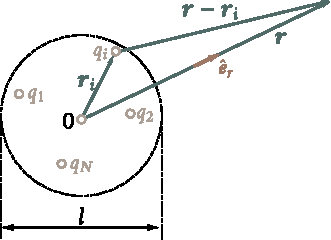
\includegraphics[scale=1]{figures/cap_01/fig_1_16.pdf}
%		\caption[]{}
%		\label{fig:1_16}
%	\end{center}
%	\vspace{-0.7cm}
%\end{figure}

A vector product is usually designated in one of two ways:
\begin{equation*}
[\vec{a},\vec{b}]\quad\text{or }\quad \vec{a}\times\vec{b}
\end{equation*}

\noindent
the latter notation resulting in the term cross product sometimes being used to signify a vector product. We shall use the latter notation\footnote{To avoid confusion, in the \LaTeX version, we shall use the cross product symbol.}. Thus, according to \eqn{1_27}, we have
\begin{equation}\label{eq:1_28}
\vecprod{a}{b} = (ab\sin\alpha)\hatvec{n}.
\end{equation}

A glance at \fig{1_16} shows that the magnitude of a vector product has a simple geometrical meaning---the expression $ab\sin\alpha$ numerically equals the area of a parallelogram constructed on the vectors being multiplied.

We determined the direction of the vector $\vecprod{a}{b}$ by relating it to the direction of rotation from the first multiplier to the second one. When considering vectors such as the position vector $\vec{r}$, the velocity $\vec{v}$, and the force $\vec{F}$, the choice of their direction is quite obvious---it follows from the nature of these quantities themselves. Such vectors are called \textbf{polar} or \textbf{true}. Vectors of the type $\vecprod{a}{b}$ whose direction is related to that of rotation are called axial or \textbf{pseudovectors}. When conditions change, for example, upon going over from a right-hand system of coordinates to a left-hand one, the directions of pseudovectors are reversed, while those of true vectors remain unchanged.

It must be borne in mind that a vector product will be a pseudovector only when both of the vectors being multiplied are true (or both are pseudovectors). The vector product of a true vector and a pseudovector will be true. Reversing of a condition determining the direction of a pseudovector will lead in this case to a change in the sign in front of the vector product and also to a change in the sign of one of the multipliers. As a result, the quantity expressed
by the vector product remains unchanged.

Since the direction of a vector product is determined by the direction of rotation from the first multiplier to the second one, the result of vector multiplication depends on the order of the multipliers. Transposition of the multipliers leads to reversing of the direction of the resultant vector. Thus, a vector product does not have the property of commutativity:
\begin{equation}\label{eq:1_29}
\vecprod{a}{b} = -\vecprod{b}{a}.
\end{equation}

\noindent
A vector product can be proved to be distributive, \ie, it can be shown that
\begin{equation}\label{eq:1_30}
\vec{a}\times(\vec{b}_1+\vec{b}_2+\ldots)] = \vec{a}\times\vec{b}_1 + \vec{a}\times\vec{b}_2 + \ldots.
\end{equation}

%\begin{figure}[t]
%	\begin{center}
%		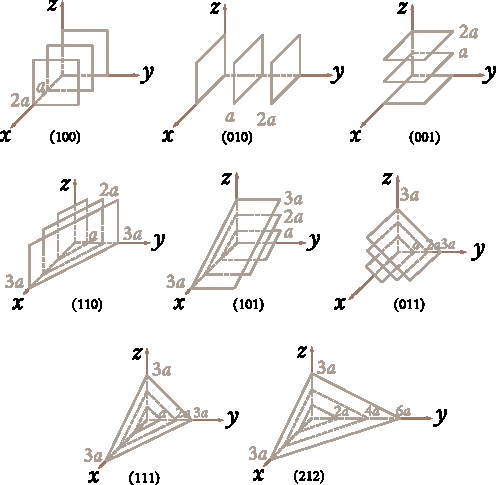
\includegraphics[scale=1]{figures/cap_01/fig_1_17.pdf}
%		\caption[]{}
%		\label{fig:1_17}
%	\end{center}
%	\vspace{-1.0cm}
%\end{figure}
\begin{figure}[t]
	\begin{minipage}[t]{0.5\linewidth}
		\begin{center}
			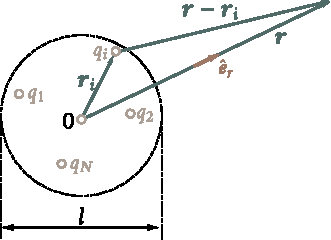
\includegraphics[scale=1]{figures/cap_01/fig_1_16.pdf}
			\caption[]{}
			\label{fig:1_16}
		\end{center}
	\end{minipage}
	\hfill{ }%\hspace{-0.1cm}
	\begin{minipage}[t]{0.5\linewidth}
		\begin{center}
			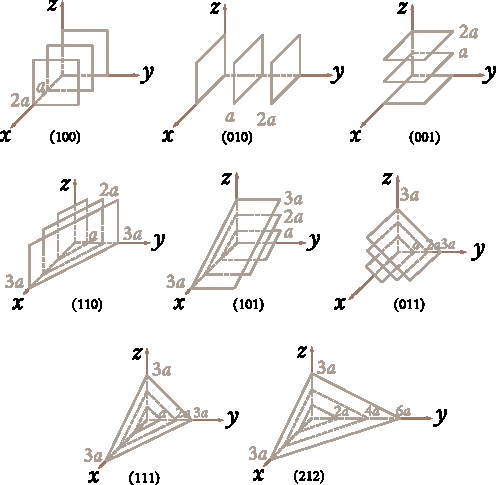
\includegraphics[scale=1]{figures/cap_01/fig_1_17.pdf}
			\caption[]{}
			\label{fig:1_17}
		\end{center}
	\end{minipage}
	\vspace{-0.3cm}
\end{figure}

Let us consider the vector products of the unit vectors of the coordinate axes (\fig{1_17}). In accordance with the definition~\eqref{eq:1_28}, we have
\begin{align}
\vecuniprod{x}{x} &= \vecuniprod{y}{y} = \vecuniprod{z}{z} = 0,\nonumber\\
\vecuniprod{x}{y} &= -\vecuniprod{y}{x} = \vecuni{z},\label{eq:1_31}\\
\vecuniprod{y}{z} &= -\vecuniprod{z}{y} = \vecuni{x},\nonumber\\
\vecuniprod{z}{x} &= -\vecuniprod{x}{z} = \vecuni{y}.\nonumber
\end{align}

\noindent
Representing the vectors being multiplied in the form of \eqn{1_9} and taking advantage of the distributivity of a vector product, we get:
\begin{align*}
\vecprod{a}{b} &= (a_x\vecuni{x}+a_y\vecuni{y}+a_z\vecuni{z})\times(b_x\vecuni{x}+b_y\vecuni{y}+b_z\vecuni{z})\\
&= a_xb_x\vecuniprod{x}{x} + a_xb_y\vecuniprod{x}{y} + a_xb_z\vecuniprod{x}{z}\\
&+ a_yb_x\vecuniprod{y}{x} + a_yb_y\vecuniprod{y}{y} + a_yb_z\vecuniprod{y}{z}\\
&+ a_zb_x\vecuniprod{z}{x} + a_zb_y\vecuniprod{z}{y} + a_zb_z\vecuniprod{z}{z}
\end{align*}

\noindent
Taking into account relation~\eqref{eq:1_31}, we arrive at the following expression:
\begin{equation}\label{eq:1_32}
\vecprod{a}{b} = \vecuni{x}(a_yb_z - a_zb_y) + \vecuni{y}(a_zb_x - a_xb_z) + \vecuni{z}(a_xb_y - a_yb_x).
\end{equation}

\noindent
The above expression can be represented in the form of a determinant
\begin{equation}\label{eq:1_33}
\vecprod{a}{b} = \begin{vmatrix}
\vecuni{x} & \vecuni{y} & \vecuni{z}\\
a_x & a_y & a_z\\
b_x & b_y & b_z
\end{vmatrix}.
\end{equation}

\begin{figure}[t]
	\begin{center}
		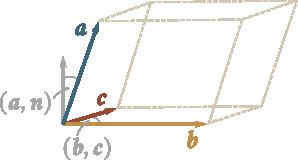
\includegraphics[scale=1]{figures/cap_01/fig_1_18.pdf}
		\caption[]{}
		\label{fig:1_18}
	\end{center}
	\vspace{-0.7cm}
\end{figure}

\textbf{Scalar Triple Product.} A scalar triple product of three vectors is defined as the expression $\vecmix{a}{b}{c}$, \ie, the scalar product of the vector $\vec{a}$ and the vector product of the vectors $\vec{b}$ and $\vec{c}$. According to the definitions~\eqref{eq:1_15} and~\eqref{eq:1_28}, we have
\begin{equation*}
\vecmix{a}{b}{c} = a\{bc\sin(\vec{b}, \vec{c})\}\cos(\vec{a},\hatvec{n}).
\end{equation*}

\noindent
Here $(\vec{b},\vec{c})$ is the angle between $\vec{b}$ and $\vec{c}$, and $(\vec{a},\hatvec{n})$ is the angle between the vector $\vec{a}$ and the unit vector $\hatvec{n}$ determining the direction of the vector $\vecprod{b}{c}$. Inspection of \fig{1_18} shows that the expression $bc\sin(\vec{b},\vec{c})$ numerically equals the area of the base of a parallelepiped constructed on the vector being multiplied, while the expression $a\cos(\vec{a},\hatvec{n})$ numerically equals the altitude of this parallelepiped taken with the plus sign if the angle $(\vec{a},\hatvec{n})$ is acute, and with the minus sign if it is obtuse. Consequently, the expression $\vecmix{a}{b}{c}$ has a simple geometrical meaning---it numerically equals the volume of a parallelepiped constructed on the vectors being multiplied [taken with the plus or minus sign depending on the value of the angle $(\vec{a},\hatvec{n})$]. In calculating the volume of a parallelepiped, the result cannot depend on which of its faces is taken as the base. Hence, it follows that
\begin{equation}\label{eq:1_34}
\vecmix{a}{b}{c} = \vecmix{b}{c}{a} = \vecmix{c}{a}{b}.
\end{equation}

\noindent
Thus, a scalar triple product permits cyclic transposition of the multipliers, \ie, substitution for each of the multipliers of the one following it in the cycle:
\begin{equation*}
\begin{tikzcd}
\vec{a}\arrow[rd] &\\
\vec{c}\arrow[u] & \arrow[l] \vec{b}
\end{tikzcd}
\end{equation*}

\textbf{Vector Triple Product.} Let us consider a vector triple product of the three vectors $\vec{a}$, $\vec{b}$ and $\vec{c}$
\begin{equation*}
\vec{d} = \vec{a}\times\vecprod{b}{c}.
\end{equation*}

\noindent
Any vector product is perpendicular to both multipliers. Therefore, the vector $\vec{d}$ is perpendicular to the unit vector $\hatvec{n}$ determining the direction of the vector $\vecprod{b}{c}$. Hence, it follows that the vector $\vec{d}$ is in the plane formed by the vectors $\vec{b}$ and $\vec{c}$ and, consequently, can be represented as a linear combination of these vectors:
\begin{equation*}
\vec{d} = \alpha\vec{b} + \beta\vec{c}
\end{equation*}

\noindent
[see \eqn{1_5}]. We find from the relevant calculations that $\alpha=\vecdot{a}{c}$ and $\beta=-\vecdot{a}{b}$. Thus,
\begin{equation}\label{eq:1_35}
\vec{a}\times\vecprod{b}{c} = \vec{b}(\vecdot{a}{c}) - \vec{c}(\vecdot{a}{b}).
\end{equation}

\textbf{Derivative of a Vector.} Let us consider a vector that changes in time according to a known law $\vec{a}(t)$. The projections of this vector onto the coordinate axes are preset functions of time. Hence,
\begin{equation}\label{eq:1_36}
\vec{a}(t) = \vecuni{x}a_x(t) + \vecuni{y}a_y(t) + \vecuni{z}a_z(t)
\end{equation}

\noindent
(we assume that the coordinate axes do not rotate in space so that their unit vectors do not change with time).

Let the vector projections receive the increments $\Delta a_x$, $\Delta a_y$, $\Delta a_z$ during the time $\Delta t$. The vector therefore receives the increment $\Delta\vec{a} = \vecuni{x}\Delta a_x + \vecuni{y}\Delta a_y + \vecuni{z}\Delta a_z$. The rate of change of the vector $\vec{a}$ with time can be characterized by the ratio of $\Delta\vec{a}$ to $\Delta t$:
\begin{equation}\label{eq:1_37}
\frac{\Delta\vec{a}}{\Delta t} = \vecuni{x}\frac{\Delta a_x}{\Delta t} + \vecuni{y}\frac{\Delta a_y}{\Delta t} + \vecuni{z}\frac{\Delta a_z}{\Delta t}.
\end{equation}

\noindent
This expression gives the mean rate of change of $\vec{a}$ during the time interval $\Delta t$. Let us assume that $\vec{a}$ changes continuously with time, without any jumps. Consequently, the smaller the interval $\Delta t$, the more accurately does the value of \eqn{1_37} characterize the rate of change in $\vec{a}$ at the moment $t$ preceding the interval $\Delta t$. Therefore, the rate of change in the vector $\vec{a}$ at the moment $t$ equals the limit of \eqn{1_37} obtained when $\Delta t$ tends to zero:
\begin{align}
\text{the rate of change in }\vec{a} &= \lim_{\Delta t\to 0}\frac{\Delta\vec{a}}{\Delta t} \nonumber\\
&= \vecuni{x} \lim_{\Delta t\to 0}\frac{\Delta a_x}{\Delta t} + \lim_{\Delta t\to 0}\vecuni{y} \frac{\Delta a_y}{\Delta t} + \lim_{\Delta t\to 0}\vecuni{z} \frac{\Delta a_z}{\Delta t}.\label{eq:1_38}
\end{align}

If there is a function $f(t)$ of the argument $t$, then the limit of the ratio of the increment of the function $\Delta f$ to the increment of the argument $\Delta t$ obtained when $\Delta t$ tends to zero is called the derivative of the function $f$ with respect to $t$ and is designated by the symbol $\diffin{f}{t}$. Expression~\eqref{eq:1_38} can therefore be written as follows:
\begin{equation}\label{eq:1_39}
\diff{\vec{a}}{t} = \vecuni{x}\diff{a_x}{t} + \vecuni{y}\diff{a_y}{t} + \vecuni{z}\diff{a_z}{t}.
\end{equation}

\noindent
The result obtained signifies that the projections of the vector $\diffin{\vec{a}}{t}$ onto the coordinate axes equal the time derivatives of the projections of the vector $\vec{a}$:
\begin{equation}\label{eq:1_40}
\left(\diff{\vec{a}}{t}\right)_{\text{pr. }x} = \diff{a_x}{t},\quad \left(\diff{\vec{a}}{t}\right)_{\text{pr. }y} = \diff{a_y}{t},\quad \left(\diff{\vec{a}}{t}\right)_{\text{pr. }z} = \diff{a_z}{t},\quad.
\end{equation}

It is customary practice in physics to denote time derivatives by the symbol of the corresponding quantity with a dot over it, for example,
\begin{equation}\label{eq:1_41}
\diff{\varphi}{t} = \dot{\varphi},\quad \diffsec{\varphi}{t} = \ddot{\varphi},\quad \diff{\vec{a}}{t} = \dot{\vec{a}},\quad \diffsec{\vec{a}}{t} = \ddot{\vec{a}}.
\end{equation}

\noindent
Using this notation, we can write equation~\eqref{eq:1_39} as follows:
\begin{equation}\label{eq:1_42}
\dot{\vec{a}} = \vecuni{x}\dot{a}_x + \vecuni{y}\dot{a}_y + \vecuni{z}\dot{a}_z.
\end{equation}

\noindent
If we take the position vector $\vec{r}(t)$ of a moving point as $\vec{a}(t)$, then by \eqn{1_42} we have
\begin{equation}\label{eq:1_43}
\dot{\vec{r}} = \vecuni{x}\dot{r}_x + \vecuni{y}\dot{r}_y + \vecuni{z}\dot{r}_z,
\end{equation}

\noindent
where $x$, $y$, $z$ are functions of $t$, namely, $x=x(t)$, $y=t(t)$, $z=z(t)$.

The differential (``increment'') of the function $f(t)$ is defined as the expression
\begin{equation}\label{eq:1_44}
\mathrm{d}f = f'\, \mathrm{d}t,
\end{equation}

\noindent
where $f'$ is the derivative of $f$ with respect to $t$.  According to \eqn{1_39}, the differential of the vector $\vec{a}$ is determined by the equation
\begin{equation}\label{eq:1_45}
\mathrm{d}\vec{a} = \vecuni{x}\mathrm{d}a_x + \vecuni{y}\mathrm{d}a_y + \vecuni{z}\mathrm{d}a_z.
\end{equation}

In particular,
\begin{equation}\label{eq:1_46}
\mathrm{d}\vec{r} = \vecuni{x}\mathrm{d}x + \vecuni{y}\mathrm{d}y + \vecuni{z}\mathrm{d}z.
\end{equation}

It must be noted that the increment of a function during a very short, but finite interval $\Delta t$ approximately equals
\begin{equation}\label{eq:1_47}
\Delta f \approx f'\Delta t = \diff{f}{t}\Delta t.
\end{equation}

\noindent
In the limit, when $\Delta t\to 0$, the approximate equation~\eqref{eq:1_47} transforms into the accurate equation~\eqref{eq:1_44}.

A similar equation to~\eqref{eq:1_47} can also be written for the vector function
\begin{equation}\label{eq:1_48}
\Delta\vec{a} \approx \diff{\vec{a}}{t}\Delta t.
\end{equation}

\textbf{Derivative of the Product of Functions.} We shall consider the function $\vec{b}(t)$ that equals the product of the scalar function $\varphi(t)$ and the vector function $\vec{a}(t)$, \ie, $\vec{b}(t)=\varphi(t)\vec{a}(t)$ or, more briefly, $\vec{b}=\varphi\vec{a}$. Let us find the increment of the function $\vec{b}$:
\begin{equation*}
\Delta\vec{b} = \Delta(\varphi\vec{a}) = (\varphi + \Delta\varphi)(\vec{a} + \Delta\vec{a}) - \varphi\vec{a} = \varphi\Delta\vec{a} + \vec{a}\Delta\varphi + \Delta\varphi\Delta\vec{a}.
\end{equation*}

\noindent
Representing the increments of the functions in the form of expressions~\eqref{eq:1_47} and~\eqref{eq:1_48}, we get:
\begin{equation*}
\Delta\vec{b} \approx \varphi\diff{\vec{a}}{t}\Delta t + \vec{a}\diff{\varphi}{t}\Delta t + \diff{\varphi}{t}\diff{\vec{a}}{t}(\Delta t)^2
\end{equation*}

\noindent
whence
\begin{equation*}
\frac{\Delta\vec{b}}{\Delta t} \approx \varphi\diff{\vec{a}}{t} + \vec{a}\diff{\varphi}{t} + \diff{\varphi}{t}\diff{\vec{a}}{t}\Delta t.
\end{equation*}

\noindent
In the limit when $\mathrm{d}t$ tends to zero, this approximate equation transforms into an accurate one. Thus,
\begin{equation*}
\diff{\vec{b}}{t} = \lim_{\Delta t\to 0} \diff{\vec{b}}{t} =  \lim_{\Delta t\to 0} \left(\varphi\diff{\vec{a}}{t} + \vec{a}\diff{\varphi}{t} + \diff{\varphi}{t} \diff{\vec{a}}{t}\Delta t\right).
\end{equation*}

\noindent
The first two addends do not depend on $\Delta t$ and therefore do not change when going over to the limit. The limit of the third addend equals zero. Hence, substituting $\varphi\vec{a}$ for $\vec{b}$, we obtain
\begin{equation}\label{eq:1_49}
\diff{(\varphi\vec{a})}{t} = \varphi\diff{\vec{a}}{t} + \vec{a}\diff{\varphi}{t} = \varphi\dot{\vec{a}}+\dot{\varphi}\vec{a}.
\end{equation}

Now let us consider the scalar product of two vector functions $\vec{a}(t)$ and $\vec{b}(t)$. The increment of this product is
\begin{align*}
\Delta(\vec{a}\vec{b}) &= (\vec{a} + \Delta\vec{a})(\vec{b} + \Delta\vec{b}) - \vec{a}\vec{b}\\
&= \vec{a}\Delta\vec{b} + \vec{b}\Delta\vec{a} + \Delta\vec{a}\Delta\vec{b} \\
&\approx \vec{a}\dot{\vec{b}}\Delta t + \vec{b}\dot{\vec{a}}\Delta t + \dot{\vec{a}}\dot{\vec{b}}(\Delta t)^2
\end{align*}

\noindent
Hence
\begin{equation*}
\diff{(\vec{a}\vec{b})}{t} = \lim_{\Delta t\to 0} \frac{\Delta(\vec{a}\vec{b})}{\Delta t} = \lim_{\Delta t\to 0} (\vec{a}\dot{\vec{b}} + \vec{b}\dot{\vec{a}} + \dot{\vec{a}}\dot{\vec{b}}\Delta t)
\end{equation*}

\noindent
or finally
\begin{equation}\label{eq:1_50}
\diff{(\vec{a}\vec{b})}{t} = \vec{a}\dot{\vec{b}} + \vec{b}\dot{\vec{a}}.
\end{equation}

\noindent
Multiplying \eqn{1_50} by $\mathrm{d}t$, we get a differential:
\begin{equation}\label{eq:1_51}
\diff{(\vec{a}\vec{b})}{t} = \vec{a}\dot{\vec{b}} + \vec{b}\dot{\vec{a}}.
\end{equation}

Let us calculate the derivative and the differential of the square of a vector function. According to Eqs.~\eqref{eq:1_50} and~\eqref{eq:1_51}, we have
\begin{align}
\diff{\vec{a}^2}{t} &= 2\vec{a}\dot{\vec{a}},\label{eq:1_52}\\
\mathrm{d}(\vec{a}^2) &= 2\vec{a}\,\mathrm{d}\vec{a},\label{eq:1_53}
\end{align}

\noindent
Taking into account that $\vec{a}^2 = a^2$ [see \eqn{1_16}], we can write:
\begin{equation}\label{eq:1_54}
2\vec{a}\,\mathrm{d}\vec{a} = \mathrm{d}(a^2) \quad \text{or} \quad \vec{a}\,\mathrm{d}\vec{a} = \mathrm{d}\left(\frac{a^2}{2}\right).
\end{equation}

Finally, let us consider the derivative of the vector product of the functions $\vec{a}(t)$ and $\vec{b}(t)$. The increment of the function being considered is
\begin{align*}
\Delta\vecprod{a}{b} &= [(\vec{a} + \Delta\vec{a}),(\vec{b} + \Delta\vec{b}) - \vecprod{a}{b}]\\
&= [\vec{a},\Delta\vec{b}] + [\Delta\vec{a},\vec{b}] + [\Delta\vec{a},\Delta\vec{b}]\\
&\approx [\vec{a},\dot{\vec{b}}\Delta t] + [\dot{\vec{a}}\Delta t,\vec{b}] + [\dot{\vec{a}}\Delta t,\dot{\vec{b}}\Delta t].
\end{align*}

\noindent
Correspondingly,
\begin{equation*}
\diff{\vecprod{a}{b}}{t} = \lim_{\Delta t\to 0} \{[\vec{a},\dot{\vec{b}}] + [\dot{\vec{a}},\vec{b}] + [\dot{\vec{a}},\dot{\vec{b}}]\Delta t\}.
\end{equation*}

\noindent
After a limit transition, we arrive at the equation
\begin{equation}\label{eq:1_55}
\diff{\vecprod{a}{b}}{t} = [\vec{a},\dot{\vec{b}}] + [\dot{\vec{a}},\vec{b}].
\end{equation}

\textbf{Derivative of a Unit Vector.} Let us consider the unit vector $\vecuni{a}$ of the vector $\vec{a}$. It is obvious that the vector $\vecuni{a}$ can change only in direction. Assume that during the very short interval $\Delta t$ the vector $\vec{a}$ and together with it the unit vector $\vecuni{a}$ rotate through the angle $\Delta\varphi$ (\fig{1_19}). At a low value of $\Delta\varphi$, the magnitude of the vector $\Delta\vecuni{a}$ approximately equals the angle $\Delta\varphi$, namely, $|\Delta\vecuni{a}|\approx\Delta\varphi$ (the segment depicting $\Delta\vecuni{a}$ is the base of an isosceles triangle with sides equal to unity). We must note that the smaller is $\Delta\varphi$, the more accurate is our approximate equation. The vector $\Delta\varphi$ itself can be represented in the form 
\begin{equation*}
\Delta\vecuni{a} = |\Delta\vecuni{a}| \boldsymbol{\cdot} \vecuni{\Delta\vec{e}} \approx \Delta\varphi \boldsymbol{\cdot} \vecuni{\Delta\vec{e}}
\end{equation*}

\noindent
where $\vecuni{\Delta\vec{e}}$ is the unit vector of the vector $\Delta\vecuni{a}$. When $\Delta\varphi$ tends to zero, the unit vector $\vecuni{\Delta\vec{e}}$ will rotate and in the limit coincide with the unit vector $\vecuni{\perp}$ perpendicular to $\vecuni{a}$ (see \fig{1_19}).

The derivative of $\vecuni{a}$ with respect to $t$, by definition, is
\begin{equation*}
\diff{\vecuni{a}}{t} = \lim_{\Delta t\to 0} \frac{\Delta\vecuni{a}}{\Delta t} = \lim_{\Delta t\to 0} \frac{\Delta\varphi}{\Delta t}\vecuni{\Delta\vec{e}} = \diff{\varphi}{t}\vecuni{\perp}.
\end{equation*}

\noindent
Thus,
\begin{equation}\label{eq:1_56}
\dot{\hat{\vec{e}}}_{a} = \dot{\varphi}\vecuni{\perp}.
\end{equation}

\noindent
The quantity $\dot{\varphi}=\diffin{\varphi}{t}$ is the angular velocity of rotation of the vector $\vec{a}$ (see Sec.~\ref{sec:1_5}). The unit vector $\vecuni{\perp}$ is in the plane in which the vector $\vec{a}$ is rotating at the given moment, and its sense is in the direction of rotation.

\begin{figure}[t]
	\begin{center}
		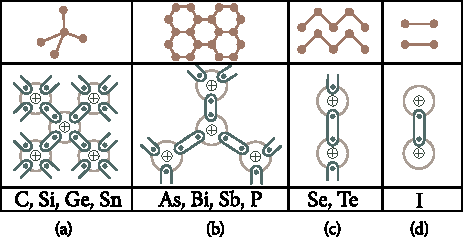
\includegraphics[scale=0.95]{figures/cap_01/fig_1_19.pdf}
		\caption[]{}
		\label{fig:1_19}
	\end{center}
	\vspace{-0.7cm}
\end{figure}

\section{Velocity and Speed}\label{sec:1_3}

A point particle in motion travels along a certain line. The latter is called its path or trajectory\footnote{It must be noted that the concept of a trajectory can be applied only to a ``classical'' particle to which accurate values of its coordinate and momentum (\ie, velocity) can be ascribed at each moment of time. According to quantum mechanics, real particles can be characterized with the aid of a coordinate and momentum only with a certain accuracy. The limit of this accuracy is determined by the equation of Heisenberg's uncertainty principle: $\Delta x\Delta p\gtrsim\hbar$. Here $\Delta x$ is the uncertainty in the coordinate of a particle, $\Delta p$ is the uncertainty in its momentum, and $\hbar$ is Planck's constant $h$ divided by $2\pi$, \ie, $\hbar = h/2\pi = \SI{1.05e-34}{\joule\second}$. The sign $\gtrsim$ signifies ``greater than a value of the order of''. Replacing the momentum with the product of the mass and the velocity, we can write $\Delta x\Delta v\gtrsim\hbar/m$. It can be seen from this relation that the smaller the mass of a particle, the more uncertain do its coordinate and velocity become, and, consequently, the less applicable is the concept of trajectory. For macroscopic bodies (\ie, bodies formed by a very great number of molecules), the uncertainties in the coordinate and velocity do not exceed the practically attainable accuracy of measuring these quantities. Hence, the concept of trajectory may be applied to such bodies without any reservations. For microparticles (electrons, protons, neutrons, separate atoms and molecules), the concept of trajectory either cannot be applied at all, or can be applied with a limited accuracy, depending on the conditions in which motion occurs. For example, the motion o electrons in a cathode-ray tube can approximately be considered as occurring along certain trajectories.}. Depending on the shape of a trajectory, we distinguish rectilinear or straight motion, circular motion, curvilinear motion, etc.

\begin{figure}[t]
	\begin{minipage}[t]{0.5\linewidth}
		\begin{center}
			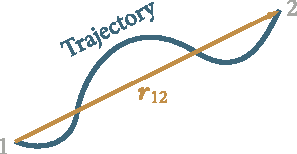
\includegraphics[scale=0.95]{figures/cap_01/fig_1_20.pdf}
			\caption[]{}
			\label{fig:1_20}
		\end{center}
	\end{minipage}
	\hfill{ }%\hspace{-0.1cm}
	\begin{minipage}[t]{0.5\linewidth}
		\begin{center}
			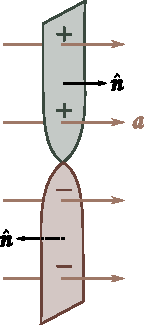
\includegraphics[scale=0.95]{figures/cap_01/fig_1_21.pdf}
			\caption[]{}
			\label{fig:1_21}
		\end{center}
	\end{minipage}
%	\vspace{-0.7cm}
\end{figure}

Assume that a point particle (in the following we shall call it simply a particle for brevity's sake) travelled along a certain trajectory from point $1$ to point $2$ (\fig{1_20}). The path between points $1$ and $2$ measured along the trajectory is called the distance travelled by the particle. We shall denote it by the symbol $s$.

The straight line between points $1$ and $2$, \ie, the shortest distance between these points, is called the displacement of the particle. We shall denote it by the symbol $\vec{r}_{12}$. Let us assume that a particle completes two successive displacements $\vec{r}_{12}$ and $\vec{r}_{23}$ (\fig{1_21}). It is natural to call such a displacement $\vec{r}_{13}$ the sum of the first two that leads to the same result as they do together. Thus, displacements are characterized by magnitude and direction and, besides, are added by using the parallelogram method. Hence, it follows that displacement is a vector.

In everyday life, we use the terms \textbf{speed} and \textbf{velocity} interchangeably, but in physics there is an important distinction between them. Speed depends on the distance travelled, and velocity on the displacement. Speed is the distance travelled by a particle in unit time. If a particle travels identical distances during equal time intervals that may be as small as desired, its motion is called uniform. In this case, the speed of the particle at each moment can be calculated by dividing the distance $s$ by the time $t$.

Velocity is a vector quantity characterizing not only how fast a particle travels along its trajectory, but also the direction in which the particle moves at each moment. Let us divide a trajectory into infinitely small portions of length $\mathrm{d}s$. An infinitely small displacement $\mathrm{d}r$ corresponds to each of these portions (\fig{1_22}). Dividing this displacement by the corresponding time interval $\mathrm{d}t$, we get the instantaneous velocity at the given point of the trajectory:
\begin{equation}\label{eq:1_57}
\vec{v} = \diff{\vec{r}}{t} = \dot{\vec{r}}.
\end{equation}

\noindent
Thus, the velocity is the derivative of the position vector of the particle with respect to time. The displacement $\mathrm{d}r$ coincides with an infinitely small element of the trajectory. Consequently, the vector $\vec{v}$ is directed along a tangent to the trajectory (see \fig{1_22}).

\begin{figure}[t]
	\begin{center}
		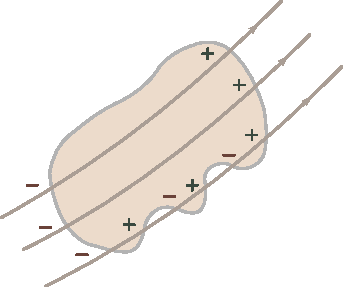
\includegraphics[scale=0.9]{figures/cap_01/fig_1_22.pdf}
		\caption[]{}
		\label{fig:1_22}
	\end{center}
\vspace{-0.7cm}
\end{figure}

Reasoning more strictly, to derive equation~\eqref{eq:1_57} we must proceed as follows.· Having fixed a certain moment of time $t$, let us consider the increment of the position vector $\Delta\vec{r}$ during the small time interval $\Delta t$\footnote{The symbol $\Delta$ (delta) is used in two cases: (a) for designating the increment of a quantity. In the case being considered, $\Delta\vec{r}$ is the increment of the position vector $\vec{r}$ during the time $\Delta t$; (b) for designating a fraction of a quantity. For example, $\Delta t$ is a fraction of the total time $t$ during which motion occurs, and $\Delta s$ is a fraction of the entire 	distance $s$ travelled by the particle.} following $t$ (\fig{1_23}). The ratio $\Delta\vec{r}/\Delta t$ gives the average value of the velocity during the time $\Delta t$. If we take smaller and smaller intervals $\Delta t$, the ratio $\Delta\vec{r}/\Delta t$ in the limit will give us the value of the velocity $\vec{v}$ at the moment $t$:
\begin{equation}\label{eq:1_58}
\vec{v} = \lim_{\Delta t\to 0} \frac{\Delta\vec{r}}{\Delta t} = \diff{\vec{r}}{t}.
\end{equation}

\noindent
We have arrived at equation~\eqref{eq:1_57}.

Let us find the magnitude of the expression~\eqref{eq:1_58}, \ie, the magnitude of the velocity $\vec{v}$:
\begin{equation}\label{eq:1_59}
v = |\vec{v}| = \left|\lim_{\Delta t\to 0} \frac{\Delta\vec{r}}{\Delta t}\right| = \lim_{\Delta t\to 0} \frac{|\Delta\vec{r}|}{\Delta t}.
\end{equation}

\noindent
We cannot write $\Delta r$ instead of $|\Delta\vec{r}|$ in this formula. The vector $\Delta\vec{r}$ is in essence the difference between two vectors ($\vec{r}$ at the moment $t+\Delta t$ minus $\vec{r}$ at the moment $t$). Therefore, its magnitude may be written only with the aid of vertical
bars [see \eqn{1_2}]. The symbol $|\Delta\vec{r}|$ signifies the magnitude of the increment of the vector $\vec{r}$, whereas $\Delta r$ is the increment of the magnitude of the vector $\vec{r}$, \ie, $\Delta|\vec{r}|$. These two quantities, generally speaking, do not equal each other:
\begin{equation*}
|\Delta\vec{r}| \neq \Delta|\vec{r}| = \Delta r.
\end{equation*}

\noindent
The following example will illustrate this. Assume that the vector $\vec{r}$ receives such an increment $\Delta\vec{r}$ that its magnitude does not change, \ie, $|\vec{r}+\Delta\vec{r}|=|\vec{r}|$ (\fig{1_24}). Consequently, the increment of the magnitude of the vector equals zero ($\Delta|\vec{r}| = \Delta r = 0$). At the same time, the magnitude of the increment of the vector $\vec{r}$, \ie, $\Delta|\vec{r}|$, differs from zero (it equals the length of $2-3$). What has been said above holds for any vector $\vec{a}$: in the general case $\Delta|\vec{a}|\neq\Delta|a|$.

\begin{figure}[t]
	\begin{minipage}[t]{0.5\linewidth}
		\begin{center}
			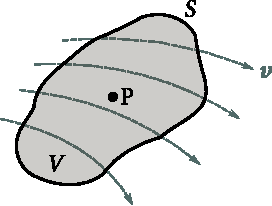
\includegraphics[scale=0.92]{figures/cap_01/fig_1_23.pdf}
			\caption[]{}
			\label{fig:1_23}
		\end{center}
	\end{minipage}
	\hfill{ }%\hspace{-0.1cm}
	\begin{minipage}[t]{0.5\linewidth}
		\begin{center}
			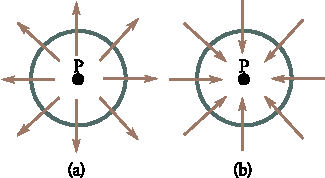
\includegraphics[scale=0.9]{figures/cap_01/fig_1_24.pdf}
			\caption[]{}
			\label{fig:1_24}
		\end{center}
	\end{minipage}
\vspace{-0.7cm}
\end{figure}

Inspection of \fig{1_23} shows that the distance $\Delta s$, generally speaking, differs in value from the magnitude of the displacement $|\Delta\vec{r}|$. If we take increments of the distance $\Delta s$ and the displacement $\Delta\vec{r}$ corresponding to smaller and smaller time intervals $\Delta t$, then the difference between $\Delta s$ and $|\Delta\vec{r}|$ will diminish, and their ratio in the limit will become equal to unity:
\begin{equation*}
\lim_{\Delta t\to 0} \frac{\Delta s}{|\Delta\vec{r}|} = 1. 
\end{equation*}

\noindent
On these grounds, we can substitute $\Delta s$ for $|\Delta\vec{r}|$ in equation~\eqref{eq:1_59}, which gives us the expression
\begin{equation}\label{eq:1_60}
v = \lim_{\Delta t\to 0} \frac{\Delta s}{\Delta t} = \diff{s}{t}. 
\end{equation}

\noindent
Thus, the magnitude of the velocity equals the derivative of the distance with respect to time.

It is evident that the quantity which in everyday life we call the speed is actually the magnitude of the velocity $\vec{v}$. In uniform motion, the magnitude of the velocity remains constant ($v=\text{constant}$), whereas the direction of the vector $\vec{v}$ changes arbitrarily (in particular it may be constant).

In accordance with \eqn{1_57}, the elementary displacement of a particle is
\begin{equation}\label{eq:1_61}
\mathrm{d}\vec{r} = \vec{v}\,\mathrm{d}{t}. 
\end{equation}

\noindent
Sometimes for clarity's sake, we shall denote an elementary displacement by the symbol $\mathrm{d}\vec{s}$, \ie, write \eqn{1_61} in the form
\begin{equation}\label{eq:1_62}
\mathrm{d}\vec{s} = \vec{v}\,\mathrm{d}{t}. 
\end{equation}

The velocity vector, like any other vector, can be represented in the form
\begin{equation}\label{eq:1_63}
\vec{v} = v_x\vecuni{x} + v_y\vecuni{y} + v_z\vecuni{z}
\end{equation}

\noindent
where $v_x, v_y, v_z$ are the projections of the vector $\vec{v}$ onto the coordinate axes. At the same time, the vector $\dot{\vec{r}}$ equal to $\vec{v}$, according to \eqn{1_43}, can be written as follows:
\vspace{-12pt}
\begin{equation}\label{eq:1_64}
\dot{\vec{r}} = \dot{x}\vecuni{x} + \dot{y}\vecuni{y} + \dot{z}\vecuni{z}
\end{equation}

\noindent
It follows from a comparison of Eqs.~\eqref{eq:1_63} and~\eqref{eq:1_64} that
\begin{equation}\label{eq:1_65}
v_x = \dot{x},\quad v_y = \dot{y},\quad v_z = \dot{z}.
\end{equation}

\noindent
Consequently, the projection of the velocity vector onto a coordinate axis equals the time derivative of the relevant coordinate of the moving particle. Taking \eqn{1_10} into account, we get:
\begin{equation}\label{eq:1_66}
v = \sqrt{\dot{x}^2 + \dot{y}^2 + \dot{z}^2}.
\end{equation}

The velocity vector can be written in the form $\vec{v}=v\vecuni{v}$, where $v$ is the magnitude of the velocity, and $\vecuni{v}$ is the unit vector of $\vec{v}$. Let us introduce the unit vector $\hatvec{\tau}$ of the tangent to a trajectory with its sense the same as that of $\vec{v}$. Hence, obviously, the unit vectors $\vecuni{v}$ and $\hatvec{\tau}$ will coincide, and we can write the following expression:
\vspace{-12pt}
\begin{equation}\label{eq:1_67}
\vec{v} = v\vecuni{v} = v\hatvec{\tau}.
\end{equation}

Let us obtain still another expression for $\vec{v}$. For this purpose, we shall introduce the position vector in the form of $\vec{r}=r\vecuni{r}$ into \eqn{1_57}. According to \eqn{1_49}, we have
\begin{equation}\label{eq:1_68}
\vec{v} = \dot{\vec{r}} = \dot{r}\vecuni{r} + r\dot{\hat{\boldsymbol{e}}}_r.
\end{equation}

\noindent
We shall limit ourselves, for simplicity, to the case when the trajectory is a plane curve, \ie, a curve such that all its points are in a single plane. Let this plane be the plane $x, y$. In \eqn{1_68}, the vector $\vec{v}$ written in the form of two components (\fig{1_25}). The first of them, which we shall designate $\vec{v}_r$, is
\begin{equation}\label{eq:1_69}
\vec{v}_r = \dot{r}\vecuni{r}.
\end{equation}

\noindent
It is directed along the position vector $\vec{r}$ and characterizes the rate of change of the magnitude of $\vec{r}$. The second component, which we shall designate $\vec{v}_{\varphi}$, is
\begin{equation}\label{eq:1_70}
\vec{v}_{\varphi} = r\dot{\hat{\boldsymbol{e}}}_r.
\end{equation}

\noindent
It characterizes the rate of change of the direction of the position vector. 

\begin{figure}[t]
	\begin{center}
		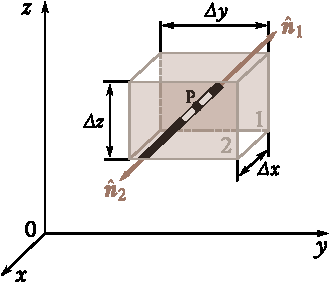
\includegraphics[scale=1]{figures/cap_01/fig_1_25.pdf}
		\caption[]{}
		\label{fig:1_25}
	\end{center}
	\vspace{-0.7cm}
\end{figure}

Using \eqn{1_56}, we can write that
\begin{equation*}
\dot{\hat{\boldsymbol{e}}}_r = \diff{\varphi}{t}\vecuni{\varphi} = \dot{\varphi}\vecuni{\varphi}
\end{equation*}

\noindent
where $\varphi$ is the angle between the position vector and the $x$-axis, and $\vecuni{\varphi}$ is a unit vector perpendicular to the position vector with its sense in the direction of growth of the angle $\varphi$ [in \eqn{1_56} the symbol $\vecuni{\perp}$ was used for this unit vector]. Using this value in \eqn{1_70}, we get:
\begin{equation}\label{eq:1_71}
\vec{v}_{\varphi} = r\dot{\varphi}\vecuni{\varphi}.
\end{equation}

\noindent
We have introduced the symbols $\vec{v}_{\varphi}$ and $\vecuni{\varphi}$ to underline the fact that the component $\vec{v}_{\varphi}$ and the corresponding unit vector are related to a change in the angle $\varphi$.

The vectors $\vec{v}_r$ and $\vec{v}_{\varphi}$ are obviously mutually perpendicular. Hence,
\begin{equation}\label{eq:1_72}
v = \sqrt{v_r^2 + v_{\varphi}^2} = \sqrt{\dot{r}^2 + r^2\dot{\varphi}^2}.
\end{equation}

Now let us consider how to calculate the distance travelled by a particle from the moment of time $t_1$ to $t_2$ if we know the speed at each moment. Let us divide the interval $t_2-t_1$ into $N$ small, but not necessarily equal intervals: $\Delta t_1$, $\Delta t_2$, \ldots, $\Delta t_N$. The total distance $s$ travelled by a particle can be represented as the sum of the distances $\Delta s_1$, $\Delta s_2$, \ldots, $\Delta s_N$ travelled during the relevant time intervals $\Delta t$:
\begin{equation*}
s = \Delta s_1 + \Delta s_2 + \ldots + \Delta s_N = \sum_{i=1}^{N} \Delta s_i.
\end{equation*}

\noindent
In accordance with \eqn{1_60}, each of the addends can approximately be represented in the form
\begin{equation*}
\Delta s_i \approx v_i \Delta t_i
\end{equation*}

\noindent
where $\Delta t_i$ is the time interval during which the distance $\Delta s_i$ was travelled, and $v_i$ is one of the values of the speed during the time $\Delta t_i$. Hence,
\begin{equation}\label{eq:1_73}
s \approx \sum_{i=1}^{N} v_i \Delta t_i.
\end{equation}

\noindent
This expression will be obeyed more accurately with diminishing time intervals $\Delta t_i$. In the limit when all the $\Delta t_i$'s tend to zero (the number of intervals $\Delta t_i$ will correspondingly grow unlimitedly), the approximate equation will become accurate:
\begin{equation*}
s = \lim_{\Delta t_i\to 0} \sum_{i=1}^{N} v_i \Delta t_i.
\end{equation*}

This expression is a definite integral of the function $v(t)$ taken within the limits from $t_1$ to $t_2$. Thus, the distance travelled by a particle during the interval from $t_1$ to $t_2$ is
\begin{equation}\label{eq:1_74}
s = \int_{t_1}^{t_2} v(t)\,\mathrm{d}t.
\end{equation}

\noindent
It must be underlined that here we are speaking of the speed. If we take an integral of the velocity $\vec{v}(t)$, we get the vector of the displacement of the particle from the point where it was at the moment $t_1$ to the point where it was at the moment $t_2$:
\begin{equation}\label{eq:1_75}
\int_{t_1}^{t_2} v(t)\,\mathrm{d}t = \int_{t_1}^{t_2} \mathrm{d}\vec{r} = \vec{r}_{12}
\end{equation}

\noindent
[see \eqn{1_61}].

If we plot the dependence of $v$ on $t$ (\fig{1_26}), then the distance travelled can be represented as the area of the figure confined between the curve $v(t)$, the straight lines $t = t_1$ and $t = t_2$, and the $t$-axis. Indeed, the product $v_i\Delta t_i$ numerically equals the area of the $i$-th strip. The sum \eqn{1_73} equals the area of the figure confined on top by the broken line formed by the top edges of all such strips. When all the $\Delta t_i$'s tend to zero, the width of a strip diminishes (their number grows simultaneously), and the broken line will coincide with the curve $v = v(t)$ in the limit. Thus, the distance travelled during the time from the moment $t_1$ to the moment $t_2$ numerically equals the area confined between the curve of the function $v = v(t)$, the time axis, and the straight lines $t = t_1$ and $t = t_2$. 

\begin{figure}[t]
	\begin{center}
		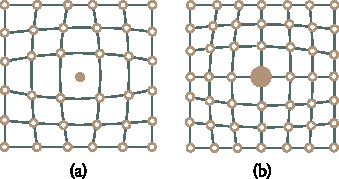
\includegraphics[scale=1]{figures/cap_01/fig_1_26.pdf}
		\caption[]{}
		\label{fig:1_26}
	\end{center}
	\vspace{-0.8cm}
\end{figure}

It should be noted that the average value of the speed during
the time from $t = t_1$ to $t = t_2$, by definition, is
\begin{equation*}
\average{v} = \frac{s}{t_2-t_1}.
\end{equation*}

\noindent
(The symbol $\langle\rangle$ embracing the $v$ indicates an average.) Introducing into this equation the expression~\eqref{eq:1_74} for $s$, we get
\begin{equation}\label{eq:1_76}
\average{v} = \frac{1}{t_2-t_1}\,\int_{t_1}^{t_2}v(t)\,\mathrm{d}t.
\end{equation}

\noindent
The average values of any scalar or vector functions are calculated in a similar way. For example, the average value of the velocity is
\begin{equation}\label{eq:1_77}
\average{\vec{v}} = \frac{1}{t_2-t_1}\,\int_{t_1}^{t_2}\vec{v}(t)\,\mathrm{d}t = \frac{\vec{r}_{12}}{t_2-t_1}.
\end{equation}

\noindent
[see \eqn{1_75}]. The average value of the function $y(x)$ within the interval from $x_1$ to $x_2$ is determined by the expression
\begin{equation}\label{eq:1_78}
\average{y} = \frac{1}{t_2-t_1}\,\int_{x_1}^{x_2}y(t)\,\mathrm{d}x.
\end{equation}

\section{Acceleration}\label{sec:1_4}

The velocity $\vec{v}$ of a particle can change with time both in magnitude and in direction. The rate of change of the vector $\vec{v}$, like the rate of change of any function of time, is determined by the derivative of the vector $\vec{v}$ with respect to $t$. Denoting this derivative by the symbol $\vec{a}$, we get:
\begin{equation}\label{eq:1_79}
\vec{a} = \lim_{\Delta t\to 0}\frac{\Delta\vec{v}}{\Delta t} = \diff{\vec{v}}{t} = \dot{\vec{v}}.
\end{equation}

\noindent
The quantity determined by equation~\eqref{eq:1_79} is called the \textbf{acceleration} of the particle.

It must be noted that the acceleration $\vec{a}$ plays the same part with respect to $\vec{v}$ as the vector $\vec{v}$ does with respect to the position vector $\vec{r}$.

Equal vectors have identical projections onto the coordinate axes. Consequently, for example,
\begin{equation*}
a_x = \left(\diff{\vec{v}}{t}\right)_{\text{pr. }\vec{x}} = \diff{v_x}{t} = \dot{v}_x
\end{equation*}

\noindent
[see Eqs.~\eqref{eq:1_40}]. At the same time according to Eqs.~\eqref{eq:1_65}, we have $v_x=\dot{x}=\diffin{x}{t}$. Therefore,
\begin{equation*}
\diff{v_x}{t} = \frac{\mathrm{d}}{\mathrm{d}t} \left(\diff{x}{t}\right) = \diffsec{x}{t} = \ddot{x}.
\end{equation*}

\noindent
What we have obtained is that the projection of the acceleration vector onto the $x$-axis equals the second derivative of the coordinate $x$ with respect to time: $a_x=\ddot{x}$. Similar expressions are obtained for the projections of the acceleration onto the $y$- and $z$-axes. Thus,
\begin{equation}\label{eq:1_80}
a_x=\ddot{x},\quad a_y=\ddot{y},\quad a_z=\ddot{z}.
\end{equation}

Using \eqn{1_67} for $\vec{v}$ in~\eqref{eq:1_79}, we get:
\begin{equation}\label{eq:1_81}
\vec{a} = \diff{(v\hatvec{\tau})}{t}.
\end{equation}

\noindent
We remind our reader that $\hatvec{\tau}$ is the unit vector of a tangent to a trajectory having the same direction as $\vec{v}$. According to \eqn{1_49},
\begin{equation}\label{eq:1_82}
\vec{a} = \dot{v}\hatvec{\tau} + v\dot{\hatvec{\tau}}.
\end{equation}

\noindent
Hence, the vector $\vec{a}$ can be represented in the form of the sum of two components. One of them has the direction $\hatvec{\tau}$, \ie, is tangent to the trajectory. It is therefore designated $\vec{a}_{\hatvec{\tau}}$ and is called the \textbf{tangential acceleration}. It equals
\begin{equation}\label{eq:1_83}
\vec{a}_{\hatvec{\tau}} = \dot{v}\hatvec{\tau}.
\end{equation}

\noindent
The second component equal to $v\dot{\hatvec{\tau}}$ is directed, as we shall show below, along a normal to the trajectory. It is therefore designated $\vec{a}_{\hatvec{n}}$ and is called the \textbf{normal acceleration}. Thus,
\begin{equation}\label{eq:1_84}
\vec{a}_{\hatvec{n}} = v\dot{\hatvec{\tau}}.
\end{equation}

In studying the properties of the two components, we shall restrict ourselves for the sake of simplicity to the case when the trajectory is a plane curve.

The magnitude of the tangential acceleration~\eqref{eq:1_83} is
\begin{equation}\label{eq:1_85}
\vec{a}_{\hatvec{\tau}} = |\dot{v}|.
\end{equation}

\noindent
If $\dot{v}>0$ (the velocity grows in magnitude), then the vector $\vec{a}_{\hatvec{\tau}}$ has the same direction as $\hatvec{\tau}$ (\ie, the same direction as $\vec{v}$). If $\dot{v}<0$ (the velocity decreases with time), then the vectors $\vec{v}$ and $\vec{a}_{\hatvec{\tau}}$ have opposite directions. In uniform motion, $\dot{v}=0$, and, therefore, tangential acceleration is absent.

To determine the properties of the normal acceleration [\eqn{1_84}], we must find out what $\dot{\hatvec{\tau}}$, \ie, the rate of change with time of the direction of a tangent to the trajectory, is determined by. It is easy to understand that this rate will grow with an increasing curvature of the trajectory and a higher velocity of a particle along it. 

The degree of bending of a plane curve is characterized by its curvature $C$ determined by the expression
\begin{equation}\label{eq:1_86}
C = \lim_{\Delta t\to 0} \frac{\Delta\varphi}{\Delta s} = \diff{\varphi}{s}
\end{equation}

\noindent
where $\Delta\varphi$ is the angle between tangents to the curve at points spaced $\Delta s$ apart (\fig{1_27}). Thus, the curvature determines the rate of turning of a tangent in motion along a curve.

\begin{figure}[t]
	\begin{center}
		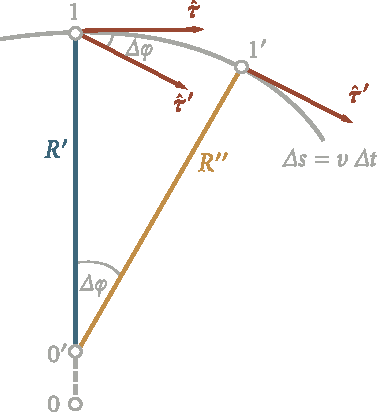
\includegraphics[scale=1]{figures/cap_01/fig_1_27.pdf}
		\caption[]{}
		\label{fig:1_27}
	\end{center}
	\vspace{-0.7cm}
\end{figure}


The reciprocal of the curvature $C$ is called the \textbf{radius of curvature} at the given point of the curve and is designated $R$:
The degree of bending of a plane curve is characterized by its curvature $C$ determined by the expression
\begin{equation}\label{eq:1_87}
R = \frac{1}{C} = \lim_{\Delta\varphi\to 0} \frac{\Delta s}{\Delta\varphi} = \diff{s}{\varphi}.
\end{equation}

\noindent
The radius of curvature is the radius of a circle that coincides at the given spot with the curve on an infinitely small portion of it. The centre of this circle is defined as the centre of curvature for the given point of the curve.

The radius and centre of curvature at point $1$ (see \fig{1_27}) can be determined as follows. Take point $1'$ near point $1$. Draw the tangents $\hatvec{\tau}$ and $\hatvec{\tau}'$ at these points. The perpendiculars to the tangents will intersect at a certain point $0'$. We must note that for a curve which is not a circle the distances $R'$ and $R''$ will differ somewhat from each other. If point $1'$ is brought closer to point $1$, the point of intersection $0'$ of the perpendiculars will move along the straight line $R'$ and in the limit will be at point $0$. It is exactly the latter that will be the centre of curvature for point $1$. The distances $R'$ and $R"$ will tend to a common limit $R$ equal to the radius of curvature. Indeed, if points $1$ and $1'$ are close to each other, we can write that $\Delta\varphi\approx\Delta s/R'$ or $R' \approx \Delta s/\Delta\varphi$. In the limit when $\Delta\varphi\to 0$, this approximate equation will transform into the strict equation $R=\diffin{s}{\varphi}$ coinciding with the definition of the radius of curvature [see \eqn{1_87}].

Let us now turn to the calculation of an [see \eqn{1_84}]. According to \eqn{1_56},
\begin{equation}\label{eq:1_88}
\dot{\hatvec{\tau}} = \diff{\varphi}{t}\hatvec{n}
\end{equation}

\noindent
where $\hatvec{n}$ is the unit vector of the normal to the trajectory with its sense in the direction of rotation of the vector $\hatvec{\tau}$ when a particle travels along the trajectory [in \eqn{1_56} a similar unit vector was designated $\vecuni{\perp}$]. The quantity $\diffin{\varphi}{t}$ can be related to the radius of curvature of the trajectory and the speed of the particle $\vec{v}$. It follows from \fig{1_27} that
\begin{equation*}
\Delta\varphi\approx \frac{\Delta s}{R'} = \frac{v'\,\Delta t}{R'}
\end{equation*}

\noindent
where $\Delta\varphi$ is the angle of rotation of the vector $\hatvec{\tau}$ during the time $\Delta t$ (coinciding with the angle between the perpendiculars $R'$ and $R''$), and $v'$ is the average speed over the distance $\Delta s$. Hence,
\begin{equation*}
\frac{\Delta\varphi}{\Delta s} \approx \frac{v'}{R'}.
\end{equation*}

\noindent
In the limit when $\Delta t$ tends to zero, the approximate equation will become a strict one, the average speed $v'$ will transform into the instantaneous speed $v$ at point $1$, and $R'$ will become the radius of curvature $R$. As a result, we get the equation
\begin{equation}\label{eq:1_89}
\diff{\varphi}{t} = \frac{v}{R} = vC
\end{equation}

\noindent
($C$ is the curvature). Hence, the rate of rotation of the velocity vector, as we assumed, is proportional to the curvature of the trajectory and the speed of a particle along its trajectory.

Using \eqn{1_89} in~\eqref{eq:1_88}, we find that $\dot{\hatvec{\tau}}=(v/R)\hatvec{n}$. And at last, introducing this expression into \eqn{1_84}, we arrive at the final equation for the normal acceleration:
\vspace{-12pt}
\begin{equation}\label{eq:1_90}
\vec{a}_{\hatvec{n}} = \diff{v^2}{R}\hatvec{n}.
\end{equation}

Thus, the acceleration vector when a particle travels along a plane curve is determined by the following expression:
\begin{equation}\label{eq:1_91}
\vec{a} = \vec{a}_{\hatvec{\tau}} + \vec{a}_{\hatvec{n}} = \dot{v}\hatvec{\tau} + \frac{v^2}{R}\hatvec{n}.
\end{equation}

\noindent
The magnitude of the vector $\vec{a}$ is
\begin{equation}\label{eq:1_92}
a = \sqrt{a_{\hatvec{\tau}}^2 + a_{\hatvec{n}}^2} = \sqrt{\dot{v}^2 + \left(\frac{v^2}{R}\right)^2}.
\end{equation}

In rectilinear motion, the normal acceleration is absent. It must be noted that an vanishes at the inflection point of a curvilinear trajectory (at point IP in \fig{1_28}). At both sides of this point, the vectors $\vec{a}_{\hatvec{n}}$ have different directions. The vector $\vec{a}_{\hatvec{n}}$ cannot change in a jump. Its direction reverses smoothly, and it becomes equal to zero at the inflection point. Assume that a particle is travelling uniformly with an acceleration constant in magnitude. Since in uniform motion the magnitude of the velocity does not change, we have $\vec{a}_{\hatvec{\tau}}=0$, so that $\vec{a}=\vec{a}_{\hatvec{n}}$. The constant magnitude of an signifies that $v^2/R=\text{constant}$. Hence, we conclude that $R=\text{constant}$ ($v=\text{constant}$ because the motion is uniform). This means that the particle is travelling along a curve of constant curvature, \ie, a circle. Thus, when the acceleration of a particle is constant in magnitude and is directed at each moment of time at right angles to the velocity vector, the trajectory of the particle will be a circle.

\begin{figure}[t]
	\begin{center}
		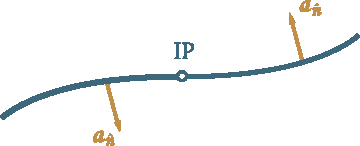
\includegraphics[scale=0.95]{figures/cap_01/fig_1_28.pdf}
		\caption[]{}
		\label{fig:1_28}
	\end{center}
	\vspace{-0.6cm}
\end{figure}

%\begin{figure}[t]
%	\begin{minipage}[t]{0.5\linewidth}
%		\begin{center}
%			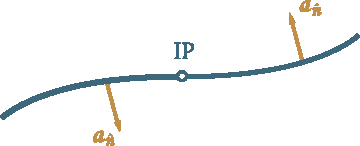
\includegraphics[scale=0.95]{figures/cap_01/fig_1_28.pdf}
%			\caption[]{}
%			\label{fig:1_28}
%		\end{center}
%	\end{minipage}
%	\hfill{ }%\hspace{-0.1cm}
%	\begin{minipage}[t]{0.5\linewidth}
%		\begin{center}
%			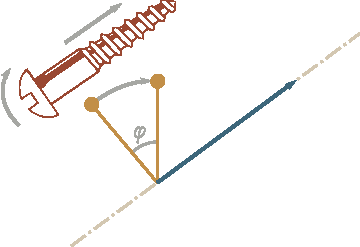
\includegraphics[scale=0.95]{figures/cap_01/fig_1_29.pdf}
%			\caption[]{}
%			\label{fig:1_29}
%		\end{center}
%	\end{minipage}
%	\vspace{-0.4cm}
%\end{figure}

\section{Circular Motion}\label{sec:1_5}

The rotation of a body through a certain angle $\varphi$ can be given in the form of a straight line whose length is $\varphi$ and whose direction coincides with the axis about which the body is rotating. To indicate the direction of rotation about a given axis, it is related to the line depicting rotation by the \textbf{right-hand screw rule}: the line should be directed so that when looking along it (\fig{1_29}) we see clockwise rotation (when rotating the head of a right-hand screw clockwise, we cause it to move away from us). We showed in Sec.~\ref{sec:1_2} (see \fig{1_4}) that rotations through finite angles are not added by the parallelogram method and are therefore not vectors. Matters are different for rotations through very small angles $\Delta\vec{\varphi}$. The distance travelled by any point of a body when rotated through a very small angle can be considered as a straight line (\fig{1_30}). Consequently, two small circular motions $\Delta\vec{\varphi}_1$ and $\Delta\vec{\varphi}_2$ performed sequentially, as can be seen from the figure, result in the same displacement $\Delta\vec{r}_3=\Delta\vec{r}_1+\Delta\vec{r}_2$ of any point of the body as the circular motion $\Delta\vec{\varphi}_3$ obtained from $\Delta\vec{\varphi}_1$ and $\Delta\vec{\varphi}_2$ by addition using the parallelogram method. Hence it follows that very small circular motions can be considered as vectors (we shall denote these vectors by $\Delta\vec{\varphi}$ or $\mathrm{d}\vec{\varphi}$). The direction of the rotation vector is associated with the direction of rotation of a body. Consequently, $\mathrm{d}\vec{\varphi}$ is not a true vector, but a pseudovector.

\begin{figure}[t]
	\begin{center}
		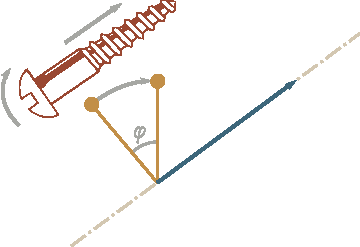
\includegraphics[scale=0.95]{figures/cap_01/fig_1_29.pdf}
		\caption[]{}
		\label{fig:1_29}
	\end{center}
	\vspace{-0.7cm}
\end{figure}

The vector quantity
\begin{equation}\label{eq:1_93}
\vec{\omega} = \lim_{\Delta t\to 0} \frac{\Delta\vec{\varphi}}{\Delta t} = \diff{\vec{\varphi}}{t}
\end{equation}

\noindent
(where $\Delta t$ is the time during which the circular motion $\Delta\vec{\varphi}$ is performed) is called the angular velocity of a body\footnote{The velocity $\vec{v}$ considered in Sec.~\ref{sec:1_3} is sometimes called linear.}. The angular velocity $\vec{\omega}$ is directed along the axis about which the body is rotating in a direction determined by the right-hand screw rule (\fig{1_31}) and is a pseudovector. The magnitude of the angular velocity, \ie, the angular speed, equals $\diffin{\varphi}{t}$. Circular motion at a constant angular velocity is called uniform. For uniform circular motion, we have $\omega=\varphi t$, where $\varphi$ is the finite angle of rotation during the time $t$ (compare with $v=s/t$). Thus, in uniform circular motion, $\omega$ shows the angle through which a body rotates in unit time.

\begin{figure}[t]
	\begin{minipage}[t]{0.5\linewidth}
		\begin{center}
			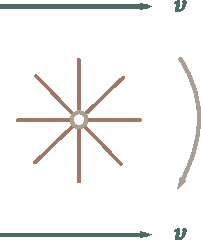
\includegraphics[scale=1]{figures/cap_01/fig_1_30.pdf}
			\caption[]{}
			\label{fig:1_30}
		\end{center}
	\end{minipage}
	\hspace{-0.1cm}
	\begin{minipage}[t]{0.5\linewidth}
		\begin{center}
			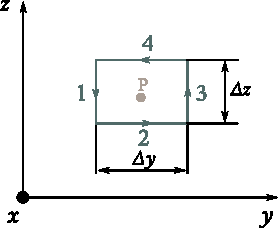
\includegraphics[scale=0.95]{figures/cap_01/fig_1_31.pdf}
			\caption[]{}
			\label{fig:1_31}
		\end{center}
	\end{minipage}
	\vspace{-0.5cm}
\end{figure}

Uniform circular motion can be characterized by the \textbf{period of revolution} $T$. It is defined as the time  during which a body completes one revolution, i.e. rotates through the angle \SI{2\pi}{\radian}, or \SI{360}{\degree}. Since the time interval $\Delta t=T$ corresponds to the angle of rotation $\Delta\varphi=2\pi$, we have
\begin{equation}\label{eq:1_94}
\omega = \frac{2\pi}{T}
\end{equation}

\noindent
whence
\begin{equation}\label{eq:1_95}
T = \frac{2\pi}{\omega}.
\end{equation}

The number of revolutions in unit time $\nu$ is evidently equal to
\begin{equation}\label{eq:1_96}
\nu = \frac{1}{T} = \frac{\omega}{2\pi}.
\end{equation}

\noindent
It follows from \eqn{1_96} that the angular velocity equals $2\pi$ multiplied by the number of revolutions per unit time:
\begin{equation}\label{eq:1_97}
\omega = 2\pi\nu.
\end{equation}

The concepts of the period of revolution and the number of revolutions per unit time can also be retained for non-uniform circular motion. Here, we must understand the instantaneous value of $T$ to signify the time during which a body would perform one revolution if it rotated uniformly with the given instantaneous value of the angular velocity, and $\nu$ to signify the number of revolutions which a body would complete in unit time in similar conditions.

The vector $\vec{\omega}$ may vary either as a result of a change in the speed of rotation of a body about its axis (in this case it changes in magnitude), or as a result of turning of the axis of rotation in space (in this case $\vec{\omega}$ changes in direction). Assume that during the time $\Delta t$ the vector $\vec{\omega}$ receives the increment $\Delta\vec{\omega}$. The change in the angular velocity vector with time is characterized by the quantity
\begin{equation}\label{eq:1_98}
\vec{\alpha} = \lim_{\Delta t\to 0} \frac{\Delta\vec{\omega}}{t} = \diff{\vec{\omega}}{t}
\end{equation}

\noindent
called the \textbf{angular acceleration}. The latter, like the angular velocity, is a pseudovector.

%\begin{figure}[t]
%	\begin{center}
%		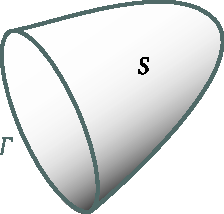
\includegraphics[scale=1]{figures/cap_01/fig_1_32.pdf}
%		\caption[]{}
%		\label{fig:1_32}
%	\end{center}
%\vspace{-0.7cm}
%\end{figure}
\begin{figure}[t]
	\begin{minipage}[t]{0.5\linewidth}
		\begin{center}
			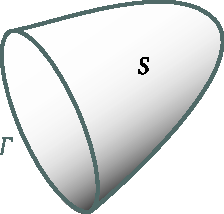
\includegraphics[scale=1]{figures/cap_01/fig_1_32.pdf}
			\caption[]{}
			\label{fig:1_32}
		\end{center}
	\end{minipage}
	\hspace{-0.1cm}
	\begin{minipage}[t]{0.5\linewidth}
		\begin{center}
			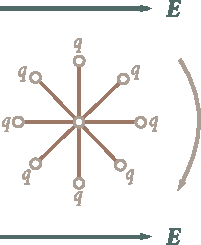
\includegraphics[scale=1]{figures/cap_01/fig_1_33.pdf}
			\caption[]{}
			\label{fig:1_33}
		\end{center}
	\end{minipage}
	\vspace{-0.6cm}
\end{figure}

Different points of a body in circular motion have different linear velocities $\vec{v}$. The velocity of each point continuously changes its direction. The speed $v$ is determined by the speed of rotation of the body $\omega$ and the distance $R$ to the point being considered from the axis of rotation. Assume that during a small interval of time the body turned through the angle $\Delta\varphi$ (\fig{1_32}). The point at the distance $R$ from the axis travels the path $\Delta s=R\Delta\varphi$. The linear speed of the point is
\begin{equation*}
v = \lim_{\Delta t\to 0} \frac{\Delta s}{\Delta t} = \lim_{\Delta t\to 0} R\frac{\Delta\varphi}{\Delta t} = R \lim_{\Delta t\to 0} \frac{\Delta\varphi}{\Delta t} = R\diff{\varphi}{t} = R\omega.
\end{equation*}

\noindent
Thus,
\begin{equation}\label{eq:1_99}
v = \omega R.
\end{equation}

Equation~\eqref{eq:1_99} relates the linear and the angular speeds. Let us find an expression relating the relevant velocities $\vec{v}$ and $\vec{\omega}$. We shall determine the position of the point of the body being considered by the position vector $\vec{r}$ drawn from the origin of coordinates on the axis of rotation (\fig{1_33}). Examination of the figure shows that the vector product $\vecprod{\omega}{r}$ coincides in direction with the vector $\vec{v}$ and its magnitude is $\omega r\sin\alpha=\omega R$. Hence,
\begin{equation}\label{eq:1_100}
\vec{v} = \vecprod{\omega}{r}.
\end{equation}

%\begin{figure}[t]
%	\begin{center}
%		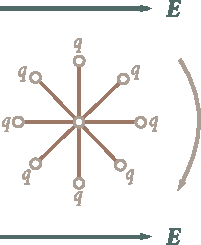
\includegraphics[scale=1]{figures/cap_01/fig_1_33.pdf}
%		\caption[]{}
%		\label{fig:1_33}
%	\end{center}
%	\vspace{-0.7cm}
%\end{figure}

The normal acceleration of the points of a rotating body is $\vec{a}_{\hatvec{n}}=v^2/R$. Introducing into this expression the value of $v$ from \eqn{1_99}, we get
\begin{equation}\label{eq:1_101}
a_{\hatvec{n}} = \omega^2 R.
\end{equation}

\noindent
If we introduce the vector $\vec{R}$ drawn to the given point of the body from the axis of rotation at right angles to the latter (see \fig{1_33}), then \eqn{1_101} can be given a vector form:
\begin{equation}\label{eq:1_102}
\vec{a}_{\hatvec{n}} = -\omega^2 \vec{R}.
\end{equation}

\noindent
There is a minus sign in this formula because the vectors $\vec{a}_{\hatvec{n}}$ and $\vec{R}$ have opposite directions.

Let us assume that the axis of rotation of a body does not turn in space. According to \eqn{1_85}, the magnitude of the tangential acceleration is $|\diffin{v}{t}|$. Using equation~\eqref{eq:1_99} and taking into account that the distance to the point being considered from the axis of rotation $R=\text{constant}$, we can write
\begin{equation*}
a_{\hatvec{\tau}} = \left| \lim_{\Delta t\to 0} \frac{\Delta v}{\Delta t} \right| = \left| \lim_{\Delta t\to 0} \frac{\Delta(\omega R)}{\Delta t} \right| = R \left| \lim_{\Delta t\to 0} \frac{\Delta(\omega)}{\Delta t} \right| = R\alpha
\end{equation*}

\noindent
where $\alpha$, is the magnitude of the angular acceleration. Consequently, the magnitude of the tangential acceleration is related to the magnitude of the angular acceleration as follows:
\begin{equation}\label{eq:1_103}
a_{\hatvec{\tau}} = \alpha R.
\end{equation}

Thus, the normal and tangential accelerations grow linearly with an increasing distance to a point from the axis of rotation.

\cleardoublepage
% !TEX root = epifanov_solid_state_physics.tex
%!TEX TS-program = pdflatex
%!TEX encoding = UTF-8 Unicode


\chapter[Mechanical Properties of Solids]{Mechanical Properties of Solids}\label{chap:2}
% \chaptermark{Bonding. The Internal Structure of Solids}

The mechanical properties---strength, hardness, ductility, wear-resistance---are the most characteristic of the properties of solids. Thanks to those properties the practical use of solids as constructional, building, electrotechnical, magnetic and other materials without which the growth of economy is impossible has become so widespread. The very names of the periods of human culture reflect the names of the solids whose mechanical properties made a qualitative leap in the process of development of human society possible---the Stone Age, the Bronze Age, the Iron Age.

This chapter deals briefly with modern physical concepts concerning the mechanical properties of solids, the laws of their plastic flow and destruction, the physical nature of strength, and prospects for the development of materials with unique mechanical properties.

\section{Elastic and plastic deformations. Hooke's law}\label{sec:13}

When a crystal is subjected to an external extension load, the distances between the atoms become greater and the atoms are displaced from their equilibrium positions in the crystal. This destroys the equilibrium between the forces of repulsion and attraction characteristic of the equilibrium state of the atoms in the lattice and results in the appearance of internal forces tending to return the atoms to their initial equilibrium positions. The value of those forces per unit cross-sectional area of the crystal is termed \textit{stress}. Let us calculate it.

It was shown in Chapter \ref{chap:1} that the energy of interaction of particles $1$ and $2$ in a solid is a function of the distance $r$ between them. This can be described by the curve $U(r)$ schematically shown in \fig{2_1}(a). When particle $2$ is displaced from its equilibrium position to a distance $x$, that is, when the distance between the particles is increased to $r=r_0+x$, the particle's energy grows and becomes $U(r)$. The change in energy $U(x)=U(r)-U(r_0)$ can be found if we expand $U(r)$ into a Taylor series in powers of $x$:
\begin{equation}\label{eq:2_1}
	U(x) = \parenthesis{\diffpartial{U}{r}}_0 x + \frac{1}{2} \parenthesis{\diffnpartial{U}{r}{2}}_0 x^2 + \frac{1}{6} \parenthesis{\diffnpartial{U}{r}{3}}_0 x^3 + \ldots .
\end{equation}

\begin{figure}[t]
	\begin{center}
		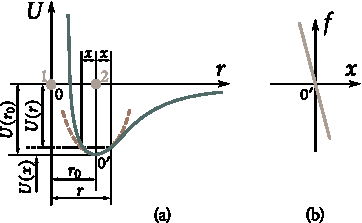
\includegraphics[scale=1.1]{figures/ch_02/fig_2_1.pdf}
		\caption[]{Variation of (a) interaction energy and (b) interaction force with the displacement of a particle from equilibrium position by a distance $x$.}
		\label{fig:2_1}
	\end{center}
	\vspace{-0.7cm}
\end{figure}

Leaving only the quadratic term of the series and taking into account the fact that $(\diffinpartial{U}{r})_0$ at point $0'$ is zero, we obtain
\begin{equation}\label{eq:2_2}
	U(x) \approx \frac{1}{2} \parenthesis{\diffnpartial{U}{r}{2}}_0 x^2 = \frac{1}{2} \beta x^2
\end{equation}

\noindent
where $\beta$ is the rigidity of the bond.

We obtained an approximate expression for the change in energy of a particle brought about by its displacement from its equilibrium position to a distance $x$. This expression is an approximation because we left only the quadratic term in the expansion \eqref{eq:2_1}, neglecting higher-order terms. Graphically this dependence is expressed by a parabola shown in \fig{2_1}(a) by a dotted line.

The force which appears between particles $1$ and $2$ when the distance between them is changed by $x$ is equal to
\begin{equation}\label{eq:2_3}
	f = - \diffpartial{U(x)}{x} = - \beta x.
\end{equation}

It follows from \eqref{eq:2_3} that the force is linearly dependent on $x$ and is directed towards the position of equilibrium, as indicated by the minus sign. It is well known that a body acted upon by such a force oscillates harmonically. Therefore such force is termed \textit{harmonic}, the same term being applied to the approximation \eqref{eq:2_2} (\textit{harmonic approximation}). Figure \ref{fig:2_1}(b) is a schematic diagram of the $f(x)$ dependence for small values of $x$. It is a straight line.

Now let us imagine that a tensile load $F$ is applied to a rod with a cross-sectional area $S$ and a length $L$. This load changes the distance between the neighbouring atomic planes $1$ and $2$ by the amount $x$ causing thereby an extension of the rod by $\Delta{L}$ (\fig{2_2}). It will be counterbalanced by the internal force $\ab{F}{int}$ equal numerically to
\begin{equation}\label{eq:2_4}
	\ab{F}{int} = f N = N \beta x
\end{equation}

\noindent
where $N$ is the number of particles in the atomic layer of area $S$.

\begin{figure}[t]
	\begin{center}
		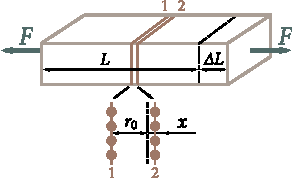
\includegraphics[scale=1.0]{figures/ch_02/fig_2_2.pdf}
		\caption[]{Uniaxial extension of a rod by an external force $F$: $1$ and $2$ are the schematic representation of adjacent atomic planes.}
		\label{fig:2_2}
	\end{center}
	\vspace{-0.7cm}
\end{figure}

The stresses a which appear in the extended rod will be
\begin{equation}\label{eq:2_5}
	\sigma = \frac{\ab{F}{int}}{S} = \frac{N}{S} \beta x = c x
\end{equation}

\noindent
where $c = N\beta/S$. Multiplying and dividing the right-hand side of \eqref{eq:2_5} by the distance between the atomic planes, $r_0$, we obtain
\begin{equation}\label{eq:2_6}
	\sigma = c r_0 \frac{x}{r_0} = E \varepsilon
\end{equation}

\noindent
where
\begin{equation}\label{eq:2_7}
	E = c r_0 = \frac{N}{S} \beta r_0
\end{equation}

\noindent
is termed the \textit{elasticity modulus,} or \textit{Young's modulus}, and
\begin{equation}\label{eq:2_8}
	\varepsilon = \frac{x}{r_0}
\end{equation}

\noindent
is the relative change in the lattice parameter in the direction of the external force $F$.

Multiplying the numerator and the denominator of \eqref{eq:2_8} by the number of atomic layers $N'$ contained in the sample of length $L$, we obtain
\begin{equation}\label{eq:2_9}
	\varepsilon = \frac{x N'}{r_0 N'} = \frac{\Delta{L}}{L}.
\end{equation}

\noindent
Hence, $\varepsilon$ is the relative elongation of the sample under the action of the external tensile load.

It follows from \eqn{2_6} that as long as the harmonic approximation remains valid, that is, as long as the forces acting between the particles displaced in relation to each other as a result of the deformation of the body remain linear functions of the displacement, the stresses $\sigma$ which appear in the body will remain proportional to the relative deformation of the body:
\begin{equation*}
	\sigma = E \varepsilon.
\end{equation*}

\noindent
The elasticity modulus $E$ serves as the proportionality factor.

Formula \eqref{eq:2_6} expresses the well-known \textit{Hooke's law}. It is valid only as long as the harmonic approximation is valid, that is, only for very small relative deformations $\varepsilon$.

The physical meaning of the elasticity modulus is quite evident from \eqn{2_6}. Putting $\varepsilon=1$, we find that $\sigma=E$. Hence, the elasticity modulus is numerically equal to the stress which is capable of causing an elongation $\Delta{L}=L$ of the sample, provided Hooke's law remains valid and the sample is not destroyed. No real material except rubber can stand such deformations.

Table \ref{table:2_1} shows the values of the elasticity modulus of some metallic crystals.

\begin{table}[!b]
	\renewcommand{\arraystretch}{1.2}
	\caption{}
	\vspace{-0.6cm}
	\label{table:2_1}
	\begin{center}\resizebox{0.84\linewidth}{!}{
			\begin{tabular}{lcccc}
				\toprule[1pt]
				\multirow{2}{*}{\textbf{Substance}} & \multicolumn{2}{c}{$E (\si{\giga\pascal})$} & \multicolumn{2}{c}{$G (\si{\giga\pascal})$}\\
				\cline{2-3} \cline{4-5}
				& \textbf{maximum} & \textbf{minimum} & \textbf{maximum} & \textbf{minimum}\\
				\midrule[0.5pt]\midrule[0.5pt]
				Aluminium	& $77$  & $64$  & $29$  & $25$\\
				Copper		& $194$ & $68$  & $77$  & $31$\\
				Iron		& $200$ & $135$ & $118$ & $60$\\
				Magnesium	& $514$ & $437$ & $184$ & $171$\\
				Tungsten	& $400$ & $400$ & $155$ & $155$\\
				Magnesium	& $126$ & $65$ & $497$ & $278$\\
				\bottomrule[1pt]
			\end{tabular}
	}\end{center}
\end{table}

It follows from data presented in Table \ref{table:2_1} that the elasticity modulus of solids is very large (of the order of \SIrange{e10}{e11}{\pascal}), which is an indication that the bonding forces in those bodies are very strong.

For some crystals the value of the elasticity modulus depends appreciably on the direction in which the lattice is deformed. Table \ref{table:2_1} shows the values of $E$ for directions in which it is at its minimum and at its maximum. For some crystals the ratio $\ab{E}{max}/\ab{E}{min}$ may be as high as $3$, pointing to a high degree of \textit{anisotropy} of such crystals.

The elasticity modulus depends only on the nature of the atoms (molecules) making up the body and on their mutual arrangement. It can be changed only by a substantial change in composition or internal structure of the solid. However, even in such cases the changes in $E$ are relatively small. Thus, high concentration alloying, heat treatment, cold rolling, etc. of steel result in great improvement in its hardness and in other mechanical properties but only in negligible (up to $10\%$) changes in its elasticity modulus; alloying copper with zinc up to $40\%$ leaves the elasticity modulus practically unchanged, although other properties experience a profound change.

We have discussed the tensile stress. However, all the considerations and the results obtained remain valid for other types of deformation---compression and shear---as well. In the latter case one should make use of the shear modulus $G$, whose values are also presented in Table \ref{table:2_1}.

When the external load is steadily increased, stress $\sigma$ and deformation $\varepsilon$ increase steadily too (\fig{2_3}). At some stress $\sigma_y$, characteristic of the specific crystal, the crystal is either destroyed or the direct proportionality between $\sigma$ and $\varepsilon$ ceases and a residual (plastic) deformation $\ab{\varepsilon}{res}$ sets in which remains after the external load has been removed. The first case is that of a brittle material and the second of a ductile one. The stress $\sigma_y$ at which a noticeable plastic flow in the body sets in is termed the \textit{yield stress} and $0$A and AB are the regions of the elastic and plastic deformations, respectively.

\begin{figure}[t]
	\begin{center}
		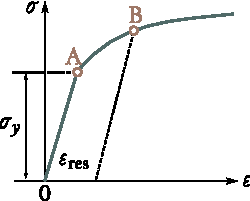
\includegraphics[scale=1.0]{figures/ch_02/fig_2_3.pdf}
		\caption[]{Typical extension curve of a ductile metal: $\sigma_y$ --- yield stress, $\ab{\varepsilon}{res}$ --- residual (plastic) deformation, $0$A---elastic deformation region, AB --- plastic deformation region.}
		\label{fig:2_3}
	\end{center}
	\vspace{-0.7cm}
\end{figure}

In brittle materials the elastic limit coincides with the tensile strength, and their destruction begins before a noticeable plastic flow sets in. In ductile metals, on the other hand, the elastic limit and the yield stress are, as a rule, much lower than the tensile strength, and these materials are destroyed only after a substantial plastic deformation has taken place.


\section{Principal laws governing plastic flow in crystals}\label{sec:14}

Residual deformations occur in all cases when the stress in ductile crystals tested for extension and compression exceeds the yield stress. However, neither extension nor compression can by themselves be the causes of such deformations. An increase in the length of the crystal can only result in an increase in the distance between the atomic planes perpendicular to the acting force. When these planes are drawn far enough apart, it may be that the forces of attraction shall no longer be able to compensate for the external load and the crystal will break. Compression can only draw the atomic planes closer together until the repulsive forces appearing between the atoms are able to counterbalance the external load. Deformation in this case is ideally elastic and cannot lead to irreversible displacement of parts of the lattice.

\begin{figure}[t]
	\begin{center}
		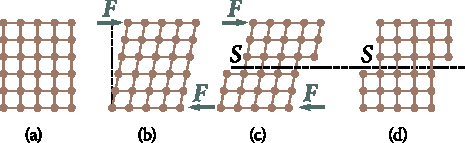
\includegraphics[scale=1.0]{figures/ch_02/fig_2_4.pdf}
		\caption[]{Crystal deformation by a shear force $\vec{F}$: (a) --- initial unstressed crystal; (b) --- elastic deformation caused by shearing stress not exceeding elastic limit; (c) --- early stages of plastic shear (slip) in the $S$ plane caused by stress exceeding elastic limit; (d) --- external force is removed, residual deformation (residual shift of one part of the lattice in relation to another) remains.}
		\label{fig:2_4}
	\end{center}
	\vspace{-0.7cm}
\end{figure}

Plastic deformation may only be the result of shearing stresses, which are able to shift some parts of the crystal in relation to the others without destroying the bonds between them. Such displacement is termed \textit{slipping}. It lies at the basis of the plastic flow process in crystalline materials. Figure \ref{fig:2_4} shows how residual deformations originate and develop in crystals [\fig{2_4}(a)] acted upon by a shearing force $\vec{F}$. As long as the elastic limit is not reached the crystal experiences elastic deformations [\fig{2_4}(b)] with the tangential stresses growing in proportion to the relative shearing deformation $\gamma$ (\textit{Hooke's law}):
\begin{equation}\label{eq:2_10}
	\tau = G \gamma
\end{equation}

\noindent
where $G$ is the shear modulus. After the crystal is relieved from external load the atoms return to their initial positions. When the elastic limit is exceeded, one part of the crystal shifts in relation to another [\fig{2_4}(c)] by one or more atomic distances along definite planes $S$ termed \textit{slip planes}. When the external load is withdrawn, the elastic stresses in the lattice vanish. However, one part of the crystal remains displaced in relation to another [\fig{2_4}(d)]. Such small irreversible displacements that proceed along numerous slip planes sum up to produce the residual deformation of the crystal as a whole.

The degree to which a crystal can be subjected to plastic deformations is determined, first of all, by the nature of the bonding forces acting between its structural elements.

The covalent bond with its rigorous directionality is appreciably weakened already by small relative displacements of the atoms. Shear destroys such bonds even before the atoms are able to establish them with other neighbouring atoms. On account of this the valence type crystals (such as diamond, silicon, germanium, antimony, bismuth, and arsenic) are incapable of plastic deformation. Outside the elastic deformation range they experience brittle destruction.

The metallic bond, which does not exhibit any directionality, on the other hand, remains practically unchanged as a result of relative tangential displacements of the atoms. This makes very great (some thousand atomic distances) relative displacements of some parts of the lattice possible, resulting in a high degree of ductility of crystals of this type.

The ionic bond occupies an intermediate position between the metallic and covalent bonds. It is less directional than the covalent bond but not so flexible as the metallic bond. Typical ionic crystals such as \ce{NaCl}, $\ce{CaF2}$, and \ce{KCl} are almost as brittle as the valence type crystals. At the same time silver chloride crystals are rather ductile.

Slipping takes place in crystals along definite crystallographic planes and directions, usually along the closest-packed planes and directions. This is because the closest-packed planes and directions are the strongest since the interatomic distances in them are the shortest and bonding is at its maximum. On the other hand, the distance between such planes is the greatest [see \eqref{eq:1_17}]; on account of this the bonding between them is at its minimum. Slipping along such planes and directions results in the minimum disarrangement in atomic order and is therefore the easiest to accomplish.

The combination of the slip plane and the slip direction, which lies in it, forms the \textit{slip system}. In the face-centered cubic lattice the slip plane coincides with the octahedral plane $(111)$ and the slip direction with the direction of the body diagonal $[111]$. In hexagonal crystals the $SS$ slip plane coincides with the base plane $(0001)$ and the $X$ slip direction with one of the three axes lying in the base plane (see \fig{2_5}, where $P$ is the external deforming load).

\begin{figure}[t]
	\begin{center}
		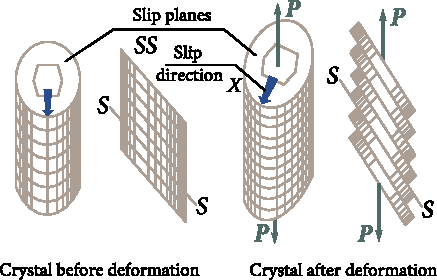
\includegraphics[scale=1.0]{figures/ch_02/fig_2_5.pdf}
		\caption[]{Slip planes and directions in a crystal.}
		\label{fig:2_5}
	\end{center}
	\vspace{-0.7cm}
\end{figure}

Numerous experiments have shown that the crystal begins to ``slip'' in the given slip system only after the shearing stress $\tau$ acting in this system reaches the critical value $\ab{\tau}{cr}$ termed the \textit{critical shearing stress}. Table \ref{table:2_2} shows the values of critical shearing stresses for some pure metallic single crystals.

\begin{table}[!b]
	\renewcommand{\arraystretch}{1.2}
	\caption{}
	\vspace{-0.6cm}
	\label{table:2_2}
	\begin{center}\resizebox{0.95\linewidth}{!}{
			\begin{tabular}{lcccc}
				\toprule[1pt]
				\textbf{Metal} & Impurity content $\parenthesis{\num{e-4}}$ & Slip plane & Slip direction & $\ab{\tau}{cr}$ $\parenthesis{\SI{e7}{\pascal}}$\\
				\midrule[0.5pt]\midrule[0.5pt]
				Cadmium	&	$0.40$	&	$(0001)$	&	$[100]$	&	$0.058$\\
				Copper	&	$10.0$	&	$(111)$		&	$[101]$	&	$0.100$\\
				Magnesium	&	$5.00$	&	$(0001)$	&	$[100]$	&	$0.083$\\
				Nickel	&	$20.0$	&	$(111)$		&	$[101]$	&	$0.580$\\
				Silver	&	$1.00$	&	$(111)$		&	$[101]$	&	$0.060$\\
				Zinc	&	$4.00$	&	$(0001)$	&	$[100]$	&	$0.094$\\
				\bottomrule[1pt]
			\end{tabular}
	}\end{center}
\end{table}

It follows from the data of \tab{2_2} that for the most ductile single crystals the critical shearing stress does not exceed \SI{e6}{\pascal}.

The critical shearing stress depends to a large extent on the prior deformation of the crystal rising with the increase in the latter. This phenomenon became known as strengthening, or \textit{cold working}. Thus a $350\%$ preliminary deformation of the magnesium single crystal increases $\ab{\tau}{cr}$ nearly $25$ times. Even greater is the effect of cold working on the cubic crystals---aluminium, copper, nickel, etc.

The strengthening of crystals is a witness to the fact that irreversible processes involving the relative displacement of atoms and of parts of the crystal take place. This results in changes of the internal energy of the crystals. Experimental study of this phenomenon has proved that the changes in the internal energy of solids in the process of their plastic deformation do, indeed, take place. Table \ref{table:2_3} shows the maximum amounts of energy that are accumulated by various metals in the process of their plastic deformation.

\begin{table}[!b]
	\renewcommand{\arraystretch}{1.2}
	\caption{}
	\vspace{-0.6cm}
	\label{table:2_3}
	\begin{center}\resizebox{0.34\linewidth}{!}{
			\begin{tabular}{lc}
				\toprule[1pt]
				\textbf{Metal} & $Q \parenthesis{\si{\joule\per\kilo\gram}}$\\
				\midrule[0.5pt]\midrule[0.5pt]
				Aluminium	&	$4400$\\
				Brass		&	$2000$\\
				Copper 		&	$2000$\\
				Iron		&	$4800$\\
				Nickel		&	$3120$\\
				\bottomrule[1pt]
			\end{tabular}
	}\end{center}
\end{table}

Should this energy be transformed into heat it would suffice to heat the metal by several degrees.

Since the accumulation of energy in the crystal in the process of its plastic deformation involves irreversible displacements of the atoms and of parts of the crystal, this energy is, in effect, the energy of \textit{residual stresses} remaining in elastically deformed parts of the crystal lattice.

Because of a higher value of internal energy in a cold worked crystal it is less thermodynamically stable than the annealed crystal. This gives rise to processes that tend to bring the crystal to the equilibrium state. Relaxation and recrystallization are two such processes.

\textit{Relaxation} consists in the dissipation of internal stresses, with the atoms of the deformed parts of the lattice returning to their regular positions. This process does not involve visible changes in the crystal structure and results in a partial or complete removal of the strengthening obtained as a result of plastic deformation. Being a diffusion-controlled process relaxation proceeds at a rate that strongly depends on temperature and on the latent heat of defect formation. Metals with a low melting point (such as tin, lead, cadmium, zinc) have comparatively high self-diffusion rates already at room temperatures. Accordingly, their relaxation rates at room temperatures are quite noticeable. At the same time there is practically no relaxation at room temperature in the metals with a high melting point; but the relaxation rate rises sharply as the temperature is increased (the relaxation process goes as far in $1$ minute at \SI{315}{\degreeCelsius} as it would in a hundred years at room temperature).

Another process that also results in the disappearance of the hardening in a cold worked crystal---the \textit{recrystallization} process---proceeds intensely at temperatures of the order of one quarter of the melting temperature of the metal (on the absolute scale). In contrast to relaxation, which produces no visible changes in the crystal structure, recrystallization involves nucleation and growth of new crystals free from internal stresses. The nucleation of such crystals takes place in the first instance in the most deformed parts of the lattice, where much of the excess free energy is concentrated. In this way, a complete change in the microscopic structure of the crystal takes place with the crystal generally going over from the single state to the polycrystalline one. In the process of recrystallization the latent heat accumulated in the deformed crystal is given off in the form of heat.

\section{Mechanical twinning}\label{sec:15}

Plastic deformation may also take the form of \textit{twinning}, which is a process of step-by-step relative displacement of atomic planes parallel to the twinning plane by a fixed distance equal to a fraction of the lattice parameter. Figure \ref{fig:2_6} shows the diagram of twinning of the crystal AECDA. The area ABCDA is the undeformed part of the crystal, BECB is the part where twinning has taken place, and BC is the \textit{twinning axis}. The positions of atoms before twinning are denoted by crosses. The plane passing through the twinning axis and separating the region of twinning from the undeformed part of the crystal is termed \textit{twinning plane}.

\begin{figure}[t]
	\begin{center}
		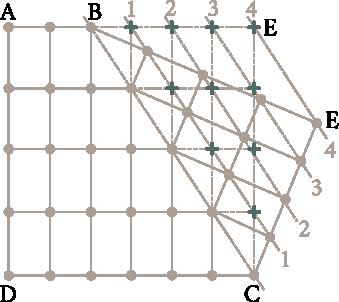
\includegraphics[scale=1.0]{figures/ch_02/fig_2_6.pdf}
		\caption[]{Twinning in a crystal: sign ``$+$'' denotes initial atomic positions in the twinning region.}
		\label{fig:2_6}
	\end{center}
	\vspace{-0.7cm}
\end{figure}

Figure \ref{fig:2_6} shows that twinning results in the displacement of the atoms of the plane $11$ relative to the twinning plane BC by a fraction of interatomic distance in the twinning direction. The plane $22$ is displaced relative to the plane $11$ by the same fraction of interatomic distance, the displacement relative to the twinning plane being twice as great. In other words, every atomic plane parallel to the twinning plane is displaced in itself by a distance proportional to its distance from the twinning plane. As a result, the atoms in the twinned region assume positions that are mirror reflections of the positions in the undeformed part of the crystal in the twinning plane.

Twinning, in the same way as slipping, may take place only along specific crystallographic planes. In case of a face-centered cubic crystal this is the $(112)$ plane, in case of a hexagonal close-packed crystal this is the $(1012)$ plane, etc. For twinning to take place the tangential stresses should exceed some critical value. The process is a very rapid one and is usually accompanied by a characteristic crackle.

Because only negligible relative displacements of the neighbouring atomic planes are involved in the process of twinning it cannot result in a great residual deformation. For instance, a complete transition of a zinc crystal to the twinned form brings about only a $7.39\%$ elongation. For this reason in crystals capable of plastic flow by means of slipping, twinning is responsible only for a negligible fraction of the total plastic deformation. In contrast to that, negligible deformation that precedes destruction of the valence crystals, in which slipping cannot take place, is due to twinning. In hexagonal crystals unfavourably oriented in relation to the external force twinning and subsequent reorientation of the crystal may result in appreciable residual deformations produced by the normal slipping process.

\section{Theoretical and real shear strengths of crystals}\label{sec:16}

Shear is the principle mechanism of plastic flow in crystals. For a long time it was presumed that such shear takes place by means of a rigid displacement of one part of the crystal in relation to another simultaneously along the entire slip plane $SS$ (\fig{2_7}).

Let us make a rough estimate of the tangential stress needed to produce such shear.

\begin{figure}[t]
	\begin{minipage}[t]{0.52\linewidth}
		\begin{center}
			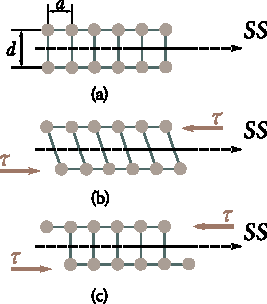
\includegraphics[scale=1]{figures/ch_02/fig_2_7.pdf}
			\caption[]{Diagram of rigid shear: (a) --- equilibrium position of atoms in atomic planes adjoining the slip plane; (b) --- gradual shift of one plane in relation to another caused by external stress $\tau$; (c) --- lower atomic plane as a whole displaced by one interatomic distance in relation to the upper plane.}
			\label{fig:2_7}
		\end{center}
	\end{minipage}
	\hfill{ }%\hspace{-0.1cm}
	\begin{minipage}[t]{0.43\linewidth}
		\begin{center}
			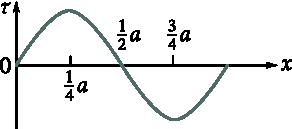
\includegraphics[scale=1]{figures/ch_02/fig_2_8.pdf}
			\caption[]{Variation of resistance to shear in the process of displacement of one part of the lattice in relation to another.}
			\label{fig:2_8}
		\end{center}
	\end{minipage}
\vspace{-0.3cm}
\end{figure}

The atoms of two adjacent parallel planes in an undeformed lattice occupy equilibrium sites corresponding to the minimum of the potential energy [\fig{2_7}(a)]. The forces acting between them are zero. As one atomic plane is displaced relative to the other tangential stresses $\tau$ appear. They resist the shear and tend to bring back the original equilibrium state [\fig{2_7}(b)]. If we assume the dependence of those stresses on the displacement to be sinusoidal (\fig{2_8}), we shall be able to express the resistance to shear in the form
\begin{equation}\label{eq:2_11}
	\tau = A \sin\parenthesis{\frac{2\pi x}{b}}
\end{equation}

\noindent
where $x$ is the displacement of the atoms from their equilibrium positions, $b=a$ the interatomic distance in the slip plane, and $A$ is a constant. For small displacements $\sin(2\pi x/b)\approx 2\pi x/b$ and therefore
\begin{equation}\label{eq:2_12}
	\tau = A \parenthesis{\frac{2\pi x}{b}}.
\end{equation}

On the other hand, for small displacements Hooke's law is valid:
\begin{equation}\label{eq:2_13}
	\tau = G \frac{x}{d}
\end{equation}

\noindent
where $G$ is the shear modulus, and $d$ the distance between the planes. From \eqref{eq:2_12} and \eqref{eq:2_13} we obtain $A=(b/d)(G/2\pi)$. Therefore
\begin{equation}\label{eq:2_14}
	\tau = \frac{b}{d} \frac{G}{2\pi} \sin\parenthesis{\frac{2\pi x}{b}}.
\end{equation}

The maximum Value $\ab{\tau}{cr}$ of the tangential stress $\tau$ is attained for $x=b/4$ and this is assumed to be the theoretical strength:
\begin{equation}\label{eq:2_15}
	\ab{\tau}{cr} = \frac{b}{d} \frac{G}{2\pi}.
\end{equation}

\noindent
Setting $b=d$, we obtain
\begin{equation}\label{eq:2_16}
	\ab{\tau}{cr} = \frac{G}{2\pi}.
\end{equation}

Hence, the critical shearing stress should be equal to about one tenth of the shear modulus. A more rigorous consideration of the nature of the bonding forces acting between the atoms leads to a negligible correction factor. The minimum value that was obtained for $\ab{\tau}{cr}$ is $G/30$. Table \ref{table:2_4} shows experimental and theoretical values of $\ab{\tau}{cr}$ for several metals.

\begin{table}[!b]
	\renewcommand{\arraystretch}{1.2}
	\caption{}
	\vspace{-0.6cm}
	\label{table:2_4}
	\begin{center}\resizebox{0.83\linewidth}{!}{
			\begin{tabular}{lcccc}
				\toprule[1pt]
				\multirow{2}{*}{\textbf{Metal}} & $\ab{\tau}{cr} \parenthesis{\SI{e7}{\pascal}}$, & \multirow{2}{*}{$G \parenthesis{\SI{e7}{\pascal}}$} & \multicolumn{2}{c}{$\ab{\tau}{cr} \parenthesis{\SI{e7}{\pascal}}$, \textbf{theory}}\\
				\cline{4-5}
				& \textbf{experiment} & & $G/(2\pi)$ & $G/30$ \\
				\midrule[0.5pt]\midrule[0.5pt]
				Cadmium & $0.06$ & $2640$ & $420$ & $88$\\
				Copper & $0.10$ & $4620$ & $735$ & $154$\\
				Iron & $2.90$ & $6900$ & $1100$ & $230$\\
				Magnesium & $0.08$ & $1770$ & $280$ & $59$\\
				Nickel & $0.58$ & $7800$ & $1240$ & $260$\\
				Silver & $0.06$ & $2910$ & $459$ & $97$\\
				Zinc & $0.09$ & $3780$ & $600$ & $126$\\
				\bottomrule[1pt]
			\end{tabular}
	}\end{center}
\end{table}

A comparison of these figures shows that the real shear strength of crystals is some $3$-$4$ orders of magnitude less than the theoretical value. This points to the fact that shear in crystals does not take place by means of a rigid relative displacement of atomic planes but by means of a mechanism involving the displacement of a comparatively small number of atoms at a time. The understanding of this fact led to the evolution of the dislocation theory of plastic flow of crystals.

\section{The dislocation concept. Principal types of dislocations}\label{sec:17}

The dislocation theory of plastic flow assumes that the slipping process starts always at imperfections in the crystal structure and develops along the shear plane by means of a gradual motion of this imperfection which at a time involves only a limited number of atoms. Such imperfections are termed \textit{dislocations}.

\textbf{Edge dislocations.} Suppose gliding took place in the crystal K in the plane ABCD in the direction of the vector $\vec{b}$ involving the area AHED (\fig{2_9}). The atomic planes on both sides from the slip plane AHED are displaced in relation to one another by the distance $b$ in the slip direction. The boundary HE separating the area AHED, where slipping took place, from the area HBCE, where slipping has not yet taken place, constitutes an edge dislocation and the vector $\vec{b}$ is termed the \textit{Burgers vector}. It describes how far slipping has proceeded in the area AHED.

\begin{figure}[t]
	\begin{minipage}[t]{0.45\linewidth}
		\begin{center}
			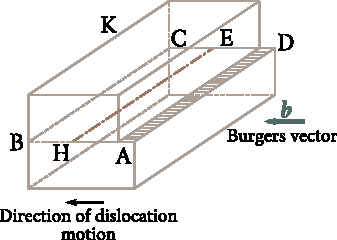
\includegraphics[scale=0.9]{figures/ch_02/fig_2_9.pdf}
			\caption[]{Shear that creates an edge dislocation. Shear took place only in region AHED of slip plane ABCD. Boundary HE is the edge dislocation.}
			\label{fig:2_9}
		\end{center}
	\end{minipage}
	\hfill{ }%\hspace{-0.1cm}
	\begin{minipage}[t]{0.51\linewidth}
		\begin{center}
			\includegraphics[scale=0.95]{figures/ch_02/fig_2_10.pdf}
			\caption[]{Arrangement of atoms in the plane perpendicular to dislocation line HE (see \fig{2_9}). Dislocation occupies the region in which lattice atoms are displaced from their equilibrium sites (bounded by a circle): $0$ --- dislocation centre; (a) --- positive dislocation; (b) negative dislocation.}
			\label{fig:2_10}
		\end{center}
	\end{minipage}
\vspace{-0.3cm}
\end{figure}

Figure \ref{fig:2_10} shows the arrangement of atoms in a plane perpendicular to the dislocation line. As a result of the shift which took place over the area AHED the upper part of the lattice contains one atomic plane (plane OM) more than the lower. Because of that the atomic row $1$ lying above the shear plane contains one atom more than the row $2$ below this plane. The interatomic distances in the upper row near the point $0$ (the dislocation centre) will accordingly be shorter than the normal value (the lattice is contracted), while the interatomic distances in the lower row near the point $0$ will be longer (the lattice is extended). As the distance to the left or to the right, and up or down, from the dislocation centre $0$ increases, the deformation of the lattice gradually subsides and at an appropriate distance from $0$ in the crystal normal disposition of atoms is restored. However, in the direction perpendicular to the plane of the diagram the dislocation passes through the entire crystal or through a considerable part of it.

Thus, a feature of the edge dislocation is the existence of an ``excess'' atomic plane OM in some part of the crystal. Therefore the process of formation of such a dislocation may be imagined as that of pulling the lattice apart and inserting an additional atomic plane in it. Such plane is termed \textit{extra plane}. If the plane is inserted into the upper part of the lattice, the edge dislocation is assumed to be positive [\fig{2_10}(a)]. But if the extra plane is inserted into the lower part of the lattice, the dislocation is assumed to be negative [\fig{2_10}(b)]. A dislocation whose Burgers vector is equal to the lattice parameter is called the \textit{unit dislocation}. When a unit dislocation passes through a cross section of the crystal, one part of it shifts in relation to the other by a distance $b$. The motion of a positive dislocation to the left causes the same shift of parts of the lattice as a motion of a negative dislocation to the right [\fig{2_10}(a,b)].

\begin{figure}[t]
	\begin{center}
		\includegraphics[scale=1.1]{figures/ch_02/fig_2_11.pdf}
		\caption[]{Formation of a screw dislocation: (a) --- shear which produces the screw dislocation. It took place in the ABCD plane. Boundary AD is a screw dislocation; (b) --- arrangement of atoms around the screw dislocation. Plane of drawing is parallel to slip plane. White circles denote atoms of the plane lying immediately above the slip plane, black circles denote atoms of the plane lying under the slip plane.}
		\label{fig:2_11}
	\end{center}
	\vspace{-0.7cm}
\end{figure}

\textbf{Screw dislocations.} Suppose an incomplete unit shift is made in the crystal K in the direction of the vector $\vec{b}$ over the area ABCD, as shown in \fig{2_11}(a); AD is the boundary of the area that experienced the shift. In \fig{2_11}(b) the white circles denote the atoms of the plane immediately above the slip plane and black circles the atoms of the plane below the slip plane. In the undeformed part of the crystal to the left of AD the atoms of those planes are arranged one on top of the other; therefore the black circles coincide with the white (this is shown by white circles with circles in the centre). In the right-hand part of the crystal, where the shift has covered one interatomic distance, that is, to the right of EH, the atoms of the planes discussed above are also arranged one on top of the other. However, in the narrow strip ADEH the atoms of the upper plane are displaced in relation to those of the lower plane the more the farther away they are from the boundary AD. This displacement results in a local deformation of the lattice, which became known as the \textit{screw dislocation}; the boundary AD is termed \textit{dislocation axis}. The origin of the term screw dislocation may be easily understood from \fig{2_12}: the motion of the atom ``a'' towards the atoms ``b, c, d, e'', etc. [\fig{2_12}(a)] lying in the plane of the screw dislocation proceeds, as may be seen from \fig{2_12}(b), along a spiral. A distinction is made between right and left screw dislocations (\fig{2_13}); the motion of both in opposite directions results in a shift in one direction.

\begin{figure}[t]
	\begin{minipage}[t]{0.5\linewidth}
		\begin{center}
			\includegraphics[scale=0.9]{figures/ch_02/fig_2_12.pdf}
			\caption[]{Explaining the origin of the ``screw dislocation'': (a) --- arrangement of atoms in a screw dislocation; (b) --- atom ``a'' moves towards atoms ``b, c, d, e'', etc. constituting the screw dislocation along a spiral.}
			\label{fig:2_12}
		\end{center}
	\end{minipage}
	\hfill{ }%\hspace{-0.1cm}
	\begin{minipage}[t]{0.46\linewidth}
		\begin{center}
			\includegraphics[scale=0.9]{figures/ch_02/fig_2_13.pdf}
			\caption[]{Arrangement of atoms in the plane perpendicular to dislocation line HE (see \fig{2_9}). Dislocation occupies the region in which lattice atoms are displaced from their equilibrium sites (bounded by a circle): $0$ --- dislocation centre; (a) --- positive dislocation; (b) negative dislocation.}
			\label{fig:2_13}
		\end{center}
	\end{minipage}
\vspace{-0.3cm}
\end{figure}

Comparing Figures \ref{fig:2_9} and \ref{fig:2_11}(a), we see that in contrast to the edge dislocation, which is perpendicular to the Burgers vector $\vec{b}$, the screw dislocation is parallel to it. The motion of the edge dislocation is in the direction of the Burgers vector $\vec{b}$, and the motion of the screw dislocation is in the direction perpendicular to it.

Recently, experimental methods for direct observation of dislocations have been developed. Figure \ref{fig:2_14}(a) shows a schematic diagram of an electron micrograph of a thin film of platinum phthalocyanine and \fig{2_14}(b,c) an electron micrograph of a copper sulphide crystal obtained with the aid of a special procedure. Dark stripes on the micrographs are the traces of the atomic planes, which in platinum phthalocyanine are arranged at a distance of \SI{12}{\angstrom} from one another and in copper sulphide at a distance of \SI{1.88}{\angstrom}. The
micrographs distinctly show the extra planes which terminate inside the crystal and form edge dislocations.

Figure \ref{fig:2_14}(d) shows an optical micrograph of a decorated screw dislocation in a $\ce{CaF2}$ crystal. The method of decoration as used for transparent crystals consists in the precipitation along their dislocation cores of impurity atoms, which make the dislocation visible in an optical microscope. The striking agreement between those pictures and the theoretical concepts as set out in Figures \ref{fig:2_10} and \ref{fig:2_12} is worthy of admiration. Points of exit of dislocations on the crystal surface may be detected with the aid of etching. When a crystal is etched in a specially selected etch, the parts of the crystal where the lattice is most deformed dissolve more readily because the atoms in those parts possess an excess energy and are chemically more active. The places of exit of dislocations on the crystal surface are just such parts. Figure \ref{fig:2_15} shows a photograph of an etched germanium surface. The dark patches are the points of exit of dislocations.

\begin{figure}[t]
	\begin{minipage}[t]{0.62\linewidth}
		\begin{center}
			\includegraphics[scale=0.8]{figures/ch_02/fig_2_14.pdf}
			\caption[]{Observation of dislocations in an electron microscope: (a) --- schematic diagram of an electron micrograph of a thin platinum phthalocyanine film (dark lines are atomic traces); (b), (c) --- electron micrograph of a copper sulfide crystal (dark lines are traces of atomic planes); (d) --- screw dislocation in a $\ce{CaF2}$ crystal obtained by decoration method.}
			\label{fig:2_14}
		\end{center}
	\end{minipage}
	\hfill{ }%\hspace{-0.1cm}
	\begin{minipage}[t]{0.34\linewidth}
		\begin{center}
			\includegraphics[scale=0.8]{figures/ch_02/fig_2_15.pdf}
			\caption[]{Etch pits on germanium surface. Dark points along the grain boundary are points of exit of dislocations.}
			\label{fig:2_15}
		\end{center}
	\end{minipage}
\vspace{-0.3cm}
\end{figure}

\section{Forces needed to move dislocations}\label{sec:18}

Suppose there is a positive dislocation with the centre at $0$, bounded at points ``a'' and ``k'' and lying in the plane $S$ in which slipping is possible [\fig{2_16}(a)]. In equilibrium the force with which the lattice acts on the dislocation is zero. This may easily be seen from the roller model shown in \fig{2_17}. The structure of the upper row of rollers which normally occupy recesses between the rollers of the lower row was deformed so that the section AB which previously contained $6$ rollers now contains only $5$. Such deformation gives rise to forces which tend to return the rollers $1, 2, 4, 5$ to their stable equilibrium positions (the forces $\vec{F}_1, \vec{F}_2, \vec{F}_3, \vec{F}_4, \vec{F}_5$). The forces applied to rollers $7, 5$ and $2, 4$ are equal in magnitude and opposite in direction.
Therefore, if the rollers of the upper row are interconnected by means of an elastic spring acting as a bond between them, the forces $\vec{F}_1$ and $\vec{F}_5, \vec{F}_2, \vec{F}_4$ will be mutually compensated and the system will be in a state of equilibrium.

\begin{figure}[t]
	\begin{center}
		\includegraphics[scale=1.2]{figures/ch_02/fig_2_16.pdf}
		\caption[]{Calculating the force needed to move a dislocation: (a) --- region of positive dislocation in crystal; $0$ is dislocation centre, ``a'' and ``k'' are dislocation boundaries, $S$ is the slip plane; (b) --- forces needed to move an atom in the dislocation region (forces applied to atoms equidistant from the dislocation centre are equal in magnitude and opposite in direction).}
		\label{fig:2_16}
	\end{center}
	\vspace{-0.7cm}
\end{figure}
\begin{figure}[t]
	\begin{center}
		\includegraphics[scale=1.0]{figures/ch_02/fig_2_17.pdf}
		\caption[]{Roller model of an edge dislocation. Forces applied to ``atoms'' $1, 5$ and $2, 4$ are equal in magnitude and opposite in direction.}
		\label{fig:2_17}
	\end{center}
	\vspace{-0.7cm}
\end{figure}

The same situation occurs in the case of a dislocation schematically shown in \fig{2_16}(b); the forces acting on atoms of the upper row occupying positions symmetrical with respect of the dislocation centre $0$ are equal in magnitude but opposite in direction (the forces $F_b=F_j, F_c=F_i, F_d=F_h, F_e=F_g$). Therefore the resultant force is zero and the dislocation is in a state of equilibrium. If, however, the dislocation moves a little in the slip plane the symmetrical arrangement of the atoms in respect of the dislocation centre will be disturbed giving rise to a force which resists the motion of the dislocation. It is evident from \fig{2_17} that this force cannot be great since the movement of the rollers $1$ and $2$ to their new equilibrium position is to a large extent the result of the action of the forces excercised on them by the rollers $4$ and $5$, which also strive to occupy positions of stable equilibrium. Calculations show the tangential stress needed to move the dislocation to be equal to
\begin{equation}\label{eq:2_17}
	\tau_0 = \frac{2G}{(1-\nu)} \exp\bracket{-\frac{2\pi b}{d(1-\nu)}}
\end{equation}

\noindent
where $G$ is the shear modulus, $\nu$ the Poisson ratio, $b$ the interatomic distance, and $d$ the distance between adjacent slip planes. The stress $\tau_0$ is the theoretical value of the critical shearing stress. Setting $b=d$ and $\nu=0.3$, we obtain $\tau_0=\num{3e-4}\,G$. Within an order of magnitude this coincides with the experimental values of $\ab{\tau}{cr}$. Thus, the theory of dislocations resolves the contradiction between the theoretical and the experimental values of shear strength of crystals.

The mechanism of motion by means of dislocations is quite frequent in nature. Snakes, worms, and shellfish move, because they generate dislocations. The motion of an earth-worm begins with the formation of an ``extension'' dislocation near the neck. The dislocation subsequently spreads along the body to the tail [\fig{2_18}(a)]. In contrast, the motion of most snakes involves the formation of a ``contraction'' dislocation near the tail and its motion towards the head [\fig{2_18}(b)].

\begin{figure}[t]
	\begin{center}
		\includegraphics[scale=1.0]{figures/ch_02/fig_2_18.pdf}
		\caption[]{Dislocation mechanism of motion of (a) an earth-worm and (b) a snake.}
		\label{fig:2_18}
	\end{center}
	\vspace{-0.7cm}
\end{figure}

\section{Sources of dislocations. Strengthening of crystals}\label{sec:19}

The dislocations in a real crystal are formed in the process of its growth from the melt or from a solution. Figure \ref{fig:2_19}(a) shows the boundaries of two blocks growing towards each other. The blocks make a small angle $\varphi$ between themselves. As the blocks fuse together, some of the atomic planes do not spread through the entire crystal but terminate at block boundaries. Those are the places where dislocations are formed [\fig{2_19}(b)]. The same situation occurs in the process of fusion of differently oriented grains in a polycrystalline sample. Since the block and grain boundaries in real solids are very extensive, the number of dislocations in them is enormous---as many as \num{e12} dislocations per square metre can be counted in well annealed metals. After cold working (rolling, drawing, etc.) dislocation densities rise to \SIrange{e15}{e16}{\per\metre\squared}. Those dislocations accumulate almost the entire energy absorbed by the metal in the process of plastic deformation.

Vacancy clusters may also serve as sources of dislocations in an undeformed crystal. Figure \ref{fig:2_20} shows an example of the formation of a positive and a negative dislocation from a cluster of vacancies.

\begin{figure}[t]
	\begin{minipage}[t]{0.51\linewidth}
		\begin{center}
			\includegraphics[scale=1]{figures/ch_02/fig_2_19.pdf}
			\caption[]{Formation of dislocations at block boundaries: (a) --- two blocks growing towards each other at an angle $\varphi$; (b) --- dislocations appearing when the blocks fuse together.}
			\label{fig:2_19}
		\end{center}
	\end{minipage}
	\hfill{ }%\hspace{-0.1cm}
	\begin{minipage}[t]{0.44\linewidth}
		\begin{center}
			\includegraphics[scale=1]{figures/ch_02/fig_2_20v.pdf}
			\caption[]{Dislocations formed from vacancy clusters: (a) --- vacancy cluster in crystal; (b) --- positive and negative dislocations formed from this cluster.}
			\label{fig:2_20}
		\end{center}
	\end{minipage}
\vspace{-0.3cm}
\end{figure}

The shear process in a crystal in response to an applied external force is, in effect, the motion of dislocations in the slip planes and their emergence through the crystal surface. Should only the dislocations already present in the crystal be responsible for this process, plastic deformation would lead to their exhaustion and to the perfection of the crystal. This is in contradiction with experience, which demonstrates that as deformation grows the lattice does not become more perfect. In fact, just the opposite is true: the density of dislocations grows in the process. It is an established fact that dislocations responsible for plastic deformation are generated in the shear process itself by the action of the external force applied to the crystal. One such generation mechanism was discovered in 1950 by F. C. Frank and W. T. Read. For the purpose of better understanding this mechanism let us consider soap bubble formation with the aid of a tube (\fig{2_21}). After the end of the tube has been immersed in a soap solution a flat film remains that closes the tube's orifice. As the air pressure in the tube is increased, the film swells and passes through the stages $1, 2, 3, 4$, etc. Until it assumes the shape of a hemisphere (stage $3$) its state is unstable: as pressure falls the film contracts striving to return to the original state $1$. After the bubble has passed stage $3$ the state of the bubble changes: it is now capable of evolution not only at a constant but also at a gradually decreasing pressure until it leaves the end of the tube. After the first bubble the second begins to be formed, followed by the third, etc.

\begin{figure}[t]
	\begin{center}
		\includegraphics[scale=1]{figures/ch_02/fig_2_21.pdf}
		\caption[]{Process of formation of a soap bubble.}
		\label{fig:2_21}
	\end{center}
	\vspace{-0.7cm}
\end{figure}

Now let us discuss the operation of the Frank-Read source. Figure \ref{fig:2_22}(a) shows an edge dislocation $DD'$ in a slip plane; points $D$ and $D'$ are fixed and do not take part in the motion of the dislocation. Dislocations may be anchored at the points of intersection with other dislocations, at impurity atoms, etc. Under the action of an external stress $\tau$ the dislocation starts bending in the same way as was the case with the soap film and at some time assumes the shape of a semicircle [\fig{2_22}(b)]. Just like the soap film the dislocation can continue to bend only if $\tau$ grows steadily until it assumes the shape of a semicircle. Its subsequent evolution takes place by itself and results in the formation of two loops [\fig{2_22}(c)], which after meeting at point C [\fig{2_22}(d)] divide the dislocation in two: an external one, which closes forming an external circle [\fig{2_22}(e)], and an internal one, which returns to the original position $DD'$. The external dislocation grows until it reaches the surface of the crystal and results in an elementary shift; the internal dislocation having returned to the initial position $DD'$ begins again to bend under the action of the applied force and to grow in the manner described above. Such process may be repeated any number of times eventually leading to a noticeable shift of one part of the crystal in relation to another in a particular slip plane.

\begin{figure}[t]
	\begin{center}
		\includegraphics[scale=1.1]{figures/ch_02/fig_2_22.pdf}
		\caption[]{Operating sequence of a Frank-Read source: (a) --- initial position of dislocation $DD'$, (b) --- acted upon by external force the dislocation bends and assumes the shape of a semicircle; (c), (d) --- further symmetric development of the dislocation loop; (e) --- formation of external closed dislocation loop spreading across the crystal and of internal dislocation $DD'$ returning to the original position.}
		\label{fig:2_22}
	\end{center}
	\vspace{-0.7cm}
\end{figure}

Low shear strength of crystals is due to the presence of innate dislocations and to the generation of others in the process of Shear. On the other hand, it is an established fact that the crystal is strengthened in the process of plastic deformation accompanied by the growth in the number of defects. The essence of such strengthening is the interaction of dislocations with each other and with other types of lattice defects causing their motion in the lattice to be obstructed.

\textbf{Interaction of dislocations.} Every dislocation, being the cause of elastic stresses of the lattice, creates a force field around itself which may be described by the values of the tangential $\tau$ and normal $\sigma$ stresses at every point. When another dislocation enters this field, forces begin to act which strive to bring the dislocations together or to move them apart. Dislocations of like signs lying in one plane are repelled, while those of opposite signs are attracted. This is the reason why, as dislocations are accumulated in a definite plane, the crystal's resistance to shear is increased and the crystal is strengthened.

\textbf{Surmounting of obstacles.} Suppose a dislocation when moving in a slip plane under the action of tangential stresses $\tau$ runs into a stationary obstacle D, for instance, an intersection with some other dislocation, an impurity atom, or some other type of defect. Figure \ref{fig:2_23} shows the method by means of which dislocation AB could, theoretically, surmount obstacle D: as the dislocation approaches D (positions $1, 2, 3$) it gradually bends forming a loop that envelops the obstacle. Behind the obstacle the loop closes and the dislocation A$'$B$'$ again becomes a straight line. Figure \ref{fig:2_24} shows a photograph illustrating a case when a dislocation runs into a stationary obstacle (dark lines represent dislocations decorated by etching). The similarity in the pictures leaves not a trace of doubt as to the validity of the theoretical pattern shown in \fig{2_23}.

\begin{figure}[t]
	\begin{minipage}[t]{0.631\linewidth}
		\begin{center}
			\includegraphics[scale=1]{figures/ch_02/fig_2_23.pdf}
			\caption[]{Schematic representation of an edge dislocation surmounting an obstacle: AB --- shape of edge dislocation away from the obstacle D; $1, 2, 3$ --- gradual bending of the dislocation as it approaches D and closing of the newly formed loop behind the obstacle; A$'$B$'$ --- straightening of the dislocation far away from the obstacle.}
			\label{fig:2_23}
		\end{center}
	\end{minipage}
	\hfill{ }%\hspace{-0.1cm}
	\begin{minipage}[t]{0.33\linewidth}
		\begin{center}
			\includegraphics[scale=0.98]{figures/ch_02/fig_2_24.pdf}
			\caption[]{Microphotographs of a chromium grain. Dark lines are etched dislocations ($\times 2000$).}
			\label{fig:2_24}
		\end{center}
	\end{minipage}
\vspace{-0.3cm}
\end{figure}

In passing around the obstacle, the length of the dislocation and the deformation of the lattice are increased, which requires additional work to be performed. Therefore, the resistance to the motion of the dislocation in the interval where it has to surmount a defect is much greater than in other parts of the lattice. This is the essence of the fact that defects strengthen a crystal. The growth in the number of dislocations in the crystal with greater plastic deformation increases the number of obstacles at points of their intersection, which is the cause of strengthening brought about by plastic deformation. Impurity atoms have a similar effect: they create local lattice imperfections and thereby hinder the motion of the dislocations, with the result that the crystal's resistance to shear is increased. Block and grain boundaries and foreign inclusions in the lattice are especially effective in hindering the motion of the dislocations. They sharply increase the resistance to the motion of dislocations and greater stresses are required to overcome their effect. The phenomenon of strengthening in the process of cold working, in the process of introducing impurity atoms (doping), and in the process of formation of inclusions (tempering, aging, etc.) is widely used in practice to improve mechanical properties of engineering materials. This method enabled the strength of the materials to be increased from $6$ to $8$ times in the last 40 years.

\section{Brittle strength of solids}\label{sec:20}

The destruction of solids may be of one of two principal types: of the \textit{brittle} and of the \textit{plastic}, or \textit{viscous}, types.

Brittle destruction takes place if the tensile strength of the material is below the elastic limit. Such a material experiences only elastic deformation prior to destruction. No irreversible changes take place in such a material before it breaks down.

In the ductile materials the elastic limit is not only below the tensile strength but also below the yield stress. Because of that the destruction process is preceded by an appreciable plastic deformation, which prepares the subsequent destruction process. In this case strength, being a typical kinetic parameter, is strongly dependent on the time the destructive stress is applied.

To begin with, let us discuss brittle strength of solids.

\textbf{Theoretical strength of solids.} There have been numerous attempts to calculate the strength of solids on the basis of molecular
interaction in them. The strength $\sigma_0$ thus calculated is termed
\textit{theoretical strength}.

Here is a glance at some of the methods of estimating $\sigma_0$.

\textit{Polanyi's method}. The simplest method of estimating the strength of solids theoretically is due to M. Polanyi. Its essence is as follows.

\begin{figure}[t]
	\begin{center}
		\includegraphics[scale=1.0]{figures/ch_02/fig_2_25.pdf}
		\caption[]{Calculating theoretical strength of solids after Polanyi (explanation in text).}
		\label{fig:2_25}
	\end{center}
	\vspace{-0.7cm}
\end{figure}

Suppose a tensile stress $\sigma$ is applied to a rod of a cross-sectional area of \SI{1}{\metre\squared} (\fig{2_25}). This stress increases the distance between the atomic planes. It is assumed that for destruction to take place a stress $\sigma_0$ able to increase the distance between the atomic planes by a value of the order of the lattice parameter $a$ should be applied. The work needed to move an atomic plane a distance $a$ away from the neighbouring plane is assumed to be equal to $\sigma_0 a$. It is further assumed that this work is transformed into the free energy of two new surfaces with a total area of \SI{2}{\metre\squared} formed as a result of the breakup, the free energy being equal to $2\alpha$, where $\alpha$ is the surface energy (``surface tension'') of the solid. Hence,
\begin{equation*}
	\sigma_0 a = 2 \alpha
\end{equation*}

\noindent
and the theoretical strength is
\begin{equation}\label{eq:2_18}
	\sigma_0 = \frac{2 \alpha}{a}.
\end{equation}

\noindent
For copper $\alpha\approx\SI{1.7}{\joule\per\metre\squared}$, $a=\SI{3.6e-10}{\metre}$, and $\sigma_0\approx\SI{e10}{\pascal}$, for silver $\alpha\approx\SI{1.14}{\joule\per\metre\squared}$, $a=\SI{4e-10}{\metre}$, and $\sigma_0=\SI{0.6e10}{\pascal}$.

\textit{Determination of $\sigma_0$ from the heat of sublimation}. The energy equal to the heat of sublimation $\ab{Q}{s}$ is required for the evaporation of a mole of a solid. For the evaporation of one molecular layer of the area of \SI{1}{\metre\squared} the required energy $W$ is a fraction of $\ab{Q}{s}$ equal to the ratio of the mass of this layer $m$ to the molar mass $M$:
\begin{equation*}
	W = \frac{\ab{Q}{s}}{m}.
\end{equation*}

\noindent
But
\begin{equation*}
	m = \ab{N}{s} \mu,\quad M = \ab{N}{A} \mu
\end{equation*}

\noindent
where $\mu$ is the molecular weight, $\ab{N}{A}=\SI{6.023e23}{\per\mole}$ the Avogadro number, and $\ab{N}{s}$ the number of molecules per square metre of the solid's surface.

For an intermolecular distance of $a$ the area per molecule is approximately equal to $a^2$ and the number of molecules per square metre
$\ab{N}{S}\approx a^2$. Therefore,
\begin{equation*}
	W = \ab{Q}{s} \frac{\ab{N}{s}}{\ab{N}{A}} \approx \frac{\ab{Q}{s}}{\ab{N}{A} a^2}.
\end{equation*}

Should the assumption be made that the evaporating molecules loose contact with the solid's surface when they are a distance of the order of the lattice parameter $a$ away from it, we would obtain for the force needed to tear away an entire surface layer as a whole
\begin{equation}\label{eq:2_19}
	\sigma_0 \approx \frac{W}{a} = \frac{\ab{Q}{s}}{\ab{N}{A}} \frac{1}{a^2}
\end{equation}

\noindent
$\sigma_0$ is assumed to be the theoretical strength of the solid.

For copper $\ab{Q}{s}=\SI{3e5}{\joule\per\mole}, a=\SI{3.6e-10}{\metre}, and \sigma_0\approx\SI{e10}{\pascal}$. Similar calculations lead to the following results: for iron $\sigma_0\approx\SI{2.3e10}{\pascal}$, for aluminium $\sigma_0\approx\SI{0.6e10}{\pascal}$, and for silver $\sigma_0\approx\SI{0.6e10}{\pascal}$.

\textit{Calculating $\sigma_0$ from the forces of molecular interaction.} Finally, let us discuss the method of calculating theoretical strength of solids from the forces of molecular interaction. Figure \ref{fig:2_26} shows the dependence of the potential energy $U(x)$ and the force of interaction between the particles $f(x)$ on the distance $x$ between them. Since it is not easy to determine the exact law governing $f(x)$, the practice is to approximate this dependence by various functions. For instance, M. Polanyi and E. Orowan used the approximation in the form of a half of a sinusoid:
\begin{equation}\label{eq:2_20}
	f(x) = \ab{f}{max} \sin\parenthesis{\frac{2\pi x}{c}}.
\end{equation}

\begin{figure}[t]
	\begin{center}
		\includegraphics[scale=1.0]{figures/ch_02/fig_2_26.pdf}
		\caption[]{Calculating theoretical strength from forces of molecular interaction (explanation in text).}
		\label{fig:2_26}
	\end{center}
	\vspace{-0.7cm}
\end{figure}

\noindent
When a body of cross-sectional area of \SI{1}{\metre\squared} is slowly torn in two, the required force is $\sigma=f\ab{N}{s}$, where $\ab{N}{s}$ is the number of particles per square metre of the cross section. Substituting $f$ from \eqref{eq:2_20} we obtain
\begin{equation}\label{eq:2_21}
	\sigma = \sigma_0 \sin\parenthesis{\frac{2\pi x}{c}}
\end{equation}

\noindent
where $\sigma_0=\ab{f}{max}\ab{N}{s}$ is the theoretical strength of the body.

For small displacements relation \eqref{eq:2_21} may be rewritten in the form
\begin{equation*}
	\sigma = \frac{\sigma_0 2\pi x}{c}.
\end{equation*}

\noindent
On the other hand, for small displacements Hooke's law is valid:
\begin{equation*}
	\sigma = \frac{E x}{c}.
\end{equation*}

Equating the right-hand sides of these equations, we obtain
\begin{equation}\label{eq:2_22}
	\sigma_0 \approx \frac{E}{2\pi} \approx 0.1 E.
\end{equation}

Calculations show that a more accurate estimate of the nature of the bonding in solids results only in a negligible correction to \eqref{eq:2_22}.

Comparing the values of theoretical strength $\sigma_0$ calculated with the aid of various methods we see that all of them yield nearly the same result whose order of magnitude is $0.1E$. Therefore it may be legitimately assumed that
\begin{equation}\label{eq:2_23}
	\sigma_0 \approx 0.1 E.
\end{equation}

\noindent
This is an enormous figure of the order of \SIrange{e9}{e10}{\pascal}.

\textbf{Real (technical) strength of solids.} The strength of real crystals and solids used for technical purposes is termed \textit{real}, or \textit{technical}, \textit{strength} $\ab{\sigma}{r}$. Table \ref{table:2_5} shows the values of the elasticity modulus $E$, of theoretical strength $\sigma_0\approx 0.1E$, of technical strength $\ab{\sigma}{r}$, and of the ratio $\sigma_0/\ab{\sigma}{r}$ for some industrial materials.

\begin{table}[!b]
	\renewcommand{\arraystretch}{1.2}
	\caption{}
	\vspace{-0.6cm}
	\label{table:2_5}
	\begin{center}\resizebox{0.98\linewidth}{!}{
			\begin{tabular}{lcccc}
				\toprule[1pt]
				\multirow{2}{*}{\textbf{Substance}} &  \textbf{Elasticity modulus} & \textbf{Theoretical strength} & \textbf{Technical strength} & \multirow{2}{*}{$\sigma_0/\ab{\sigma}{r}$}\\
				& $E\,\parenthesis{\SI{e7}{\pascal}}$ & $\sigma_0\approx 0.1E \parenthesis{\SI{e7}{\pascal}}$ & $\ab{\sigma}{r} \parenthesis{\SI{e7}{\pascal}}$ & \\
				\midrule[0.5pt]\midrule[0.5pt]
				Aluminium & $6000$ & $600$ & $9.0$ & $65$\\
				Copper & $12000$ & $1200$ & $23$ & $50$\\
				Glass & $8000$ & $800$ & $8.0$ & $100$\\
				Iron & $21000$ & $2100$ & $30$ & $70$\\
				Rock salt & $4000$ & $400$ & $0.5$ & $800$\\
				Silver & $8000$ & $800$ & $18$ & $45$\\
				\bottomrule[1pt]
			\end{tabular}
	}\end{center}
\end{table}

It follows from the data of \tab{2_5} that the technical strength of solids is from $2$ to $3$ orders of magnitude less than their theoretical
strength.

At present there is a general agreement that such discrepancy between $\sigma_0$ and $\ab{\sigma}{r}$ is due to the presence of defects in real solids of various types, in particular of microscopic cracks which reduce the strength of solids. This is accounted for by the so-called \textit{Griffith theory}. Let us calculate the technical strength using this theory.

We take a sample in the form of a thin plate and apply a tensile stress $\sigma$ to it [\fig{2_27}(a)]. The density of elastic energy in such an elastically extended sample is $\sigma^2/(2E)$\footnote{Indeed, the relative deformation in a sample under stress a is $\varepsilon=\sigma/E$, the absolute deformation $\Delta{L}=\varepsilon L$ ($L$ being the length of the sample). The work performed by the stress $\sigma$ to extend the sample by $\Delta{L}$ is $(1/2)\sigma S\Delta{L}=\sigma^2SL/(2E)=\sigma^2V/(2E)$ ($S$ is the cross-sectional area and $V$ the volume of the sample). This work is transformed into the elastic energy of the sample of volume $V$. Therefore, the specific volume density of the elastic energy is $\sigma^2/(2E)$.}.

Now let us imagine that a transverse microscopic crack of the length $l$ running through the entire thickness $\delta$ of the sample has developed in it. The appearance of the crack is accompanied by the formation of a free surface $S\approx 2l\delta$ inside the sample and by an increase in the sample's energy by the amount $\Delta{U}_1\approx 2l\delta\alpha$ ($\alpha$ is the free surface energy of the sample per unit area). On the other hand, the formation of a crack relieves the elastic stress from the volume $V\approx l^2\delta$ of the sample, whereby its elastic energy is reduced by the amount $\Delta{U}_2\approx l^2\delta\sigma^2/(2E)$. The total change in the energy of the sample $W(l)$ brought about by the appearance of a crack in it is
\begin{equation}\label{eq:2_24}
	W(l) = 2 l \delta \alpha - l^2 \delta \frac{\sigma^2}{2E}.
\end{equation}

Figure \ref{fig:2_27}(b) shows the dependence of $W$ on the length $l$ of the crack. It has a maximum where its derivative vanishes: $\diffin{W}{l}=2\delta\alpha-l\delta\sigma^2/E$. Denote the length of the crack corresponding to the maximum energy by $\ab{l}{cr}$. We obtain from the last relation
\begin{equation}\label{eq:2_25}
	\ab{l}{cr} = \frac{2 \alpha E}{\sigma^2}.
\end{equation}

\begin{figure}[t]
	\begin{center}
		\includegraphics[scale=1.0]{figures/ch_02/fig_2_27.pdf}
		\caption[]{The Griffith theory of calculating the real strength of solids (explanation in text).}
		\label{fig:2_27}
	\end{center}
	\vspace{-0.7cm}
\end{figure}

It may be seen from \fig{2_27}(b) that as long as the length $l$ of the crack remains below the critical value $\ab{l}{cr}$, energy is needed for it to develop. On the other hand, starting with $l=\ab{l}{cr}$ further extension of the sample results in a reduction in its energy. Therefore, it takes place spontaneously with the brittle destruction of the sample as the final result.

Hence, the technical strength of solids having microscopic cracks should be calculated according to the Griffith theory from relation \eqref{eq:2_25}:
\begin{equation}\label{eq:2_26}
	\ab{\sigma}{r} \approx \parenthesis{\frac{2\alpha E}{l}}^{1/2} \approx \beta \parenthesis{\frac{\alpha E}{l}}^{1/2}.
\end{equation}

\noindent
This result was subsequently verified by many investigators for various quite different methods of applying loads to the sample. A negligible difference was observed only in case of the numerical coefficient $\beta$.

Should we substitute the values of $\alpha, E, \ab{\sigma}{r}$ for copper ($\alpha\approx\SI{1.7}{\joule\per\metre\squared}, E=\SI{1.2e11}{\pascal}, \ab{\sigma}{r}=\SI{1.8e8}{\pascal}$) into \eqref{eq:2_26}, we would obtain $l\approx\SI{8e-6}{\metre}$. Approximately the same values of $l$ may be obtained for other solids.

It follows that for the strength of the solids to be reduced from the theoretical value to the value of the technical strength microscopic cracks of the order of several micrometers in length should develop in them up to the moment preceding their destruction. Many factors may be the cause of such cracks.

The cracks may be produced in the course of the production of the solid, especially in the course of its mechanical processing. A proof of this is, in particular, a significant dependence of the strength of the sample on its dimensions, especially in the small dimensions range. Thus the strength of a glass filament of \SI{2.5}{\micro\metre} in diameter is almost $100$ times that of a massive sample. The explanation is that as the dimensions of the sample are reduced so too is the probability of a large crack responsible for low strength appearing in it. Such dependence of the strength on the dimensions of the sample became known as the \textit{scale factor}. The cracks may be the result of a large number of vacancies merging together.

Figure \ref{fig:2_28} shows a dislocation mechanism of crack production. Dislocations of a similar sign move in slip plane SS and meeting obstacle B begin to accumulate in its vicinity. Large stresses able to produce cracks $l$ may develop at the head of this dislocation pile-up.

\begin{figure}[t]
	\begin{center}
		\includegraphics[scale=1.0]{figures/ch_02/fig_2_28.pdf}
		\caption[]{Formation of a crack near a dislocation pile-up.}
		\label{fig:2_28}
	\end{center}
	\vspace{-0.7cm}
\end{figure}

\section{Time dependence of fhe strength of solids}\label{sec:21}

The theory of strength based on the condition \eqref{eq:2_26} and discussed above describes actually the final stage of the destructive process when the body already contains cracks able to cause brittle rupture.

However, the initial stages of the destructive process during which the cracks originate and grow to attain critical dimensions $\ab{l}{cr}$ are also important. This process is a gradual one and takes time $\tau$ to be completed. The time $\tau$ that it takes for the destructive process to develop from the moment the load is applied to the body to the moment
of rupture is termed the \textit{durability} of the material.

The firsts experiments aimed at investigating durability were carried out by S. N. Zhurkov and G. M. Bartenev with coworkers. They also developed modern notions about the physical nature of durability.

It was established by experiments that the durability $\tau$, the tensile stress $\sigma$, and the absolute temperature $T$ are related by the expression:
\begin{equation}\label{eq:2_27}
	\tau = \tau_0 e^{(U_0 - \gamma\sigma)/(\ab{k}{B} T)}
\end{equation}

\noindent
where $\tau_0, U_0$, and $\gamma$ are constants dependent on the nature and structure of the body.

For $T = $constant, formula \eqref{eq:2_27} may be rewritten in the form
\begin{equation}\label{eq:2_28}
	\tau = A e^{-\beta\sigma}
\end{equation}

\noindent
where $A=\tau_0 e^{U_0/(\ab{k}{B} T)}$, and $\beta=\gamma/(\ab{k}{B} T)$.

Formulae \eqref{eq:2_27} and \eqref{eq:2_28} were tested on a great number of different materials (metals, polymers, haloid compounds, etc.) in an $8$ to $10$ order of magnitude range of the values of $\tau$ and in a wide range of the values of $T$.

\begin{figure}[t]
	\begin{center}
		\includegraphics[scale=1.0]{figures/ch_02/fig_2_29.pdf}
		\caption[]{Durability versus stress for aluminium ($1$), Plexiglas ($2$), and silver chloride ($3$).}
		\label{fig:2_29}
	\end{center}
	\vspace{-0.7cm}
\end{figure}

Figure \ref{fig:2_29} shows the dependence of the durabilities $\tau$ of aluminium ($1$), Plexiglas ($2$), and silver chloride ($3$) on the applied stress $\sigma$ at various temperatures expressed in the $\log{\tau}$ versus $\sigma$ coordinate system. It may be seen from \fig{2_29} that the dependence $\tau(\sigma)$ in semilogarithmic coordinates is well represented by a straight line. A family of such straight lines obtained for a given material at different temperatures resembles a fan with the apex at some point called pole.
It follows from \eqn{2_27} that $\tau$ will be independent of $T$ and that the straight lines $\log{\tau(\sigma)}$ at different temperatures will intersect at one point (at the pole) only if $U_0-\gamma\sigma=0$; but in that case $\log{\tau}=\log{\tau_0}$. Hence, the pole should be at a distance $\log{\tau_0}$ below the $\sigma$-axis.

It is evident from \fig{2_29} that the poles for all the materials tested lie practically on the same straight line parallel to the $\sigma$-axis. This means that $\tau_0$ is approximately the same for all the materials. Experiments show it to be of the order of \SIrange{e-12}{e-13}{\second}, that is, close to the period of oscillations of atoms in solids.

Let us take the logarithm of \eqref{eq:2_27}:
\begin{equation}\label{eq:2_29}
	\log{\tau} = \log{\tau_0} + \frac{(U_0 - \gamma\sigma)}{\ab{k}{B}T} = \log{\tau_0} + \frac{U}{\ab{k}{B}T},\quad U = U_0 - \gamma\sigma.
\end{equation}

\noindent
Measuring the dependence of $\log{\tau}$ on $1/T$ for constant values of $\sigma$, we can determine $U$ for various values of the stress $\sigma$ experimentally; the dimensions of $U$ are that of energy and because of this it is termed \textit{activation energy of the destructive process}. Figure \ref{fig:2_30} shows the dependence of the activation energy of rupture of viscose fibre on stress for various temperatures.
It may be seen that $U$ is independent of $T$ and is determined solely by $\sigma$; for $\sigma=0$ the maximum value of $U$ is $U_0\approx\SI{40}{\kilo\cal\per\mole}$; for a stress $\sigma\approx\SI{107e7}{\pascal}$ we see that $U=0$.
Figure \ref{fig:2_31} shows that for $\sigma\approx\SI{107e7}{\pascal}$ a practically instantaneous rupture of viscous fibre takes place (during the time $\tau_0$), no matter what its temperature is.

\begin{figure}[t]
	\begin{minipage}[t]{0.48\linewidth}
		\begin{center}
			\includegraphics[scale=1]{figures/ch_02/fig_2_30.pdf}
			\caption[]{Activation energy of rupture of viscose fibre at different temperatures (triangles, $-\SI{76}{\degreeCelsius}$; circles, $+\SI{20}{\degreeCelsius}$; crosses, $+\SI{80}{\degreeCelsius}$) versus stress.}
			\label{fig:2_30}
		\end{center}
	\end{minipage}
	\hfill{ }%\hspace{-0.1cm}
	\begin{minipage}[t]{0.48\linewidth}
		\begin{center}
			\includegraphics[scale=1]{figures/ch_02/fig_2_31.pdf}
			\caption[]{Durability of viscose fibre at different temperatures versus stress.}
			\label{fig:2_31}
		\end{center}
	\end{minipage}
\vspace{-0.3cm}
\end{figure}

Meticulous experiments carried out by S. N. Zhurkov with coworkers and by other investigators on a variety of materials demonstrated that for metals $U_0$ is quite close to the sublimation energy $\ab{Q}{s}$ and for polymers to the thermal destruction energy $\ab{Q}{d}$. Table \ref{table:2_6} shows the values of $U_0, \ab{Q}{s}$, and $\ab{Q}{d}$ for some materials. It may be seen that $U_0$ coincides either with $\ab{Q}{s}$ or with $\ab{Q}{d}$ with a high degree of accuracy.

\begin{table}[!b]
	\renewcommand{\arraystretch}{1.2}
	\caption{}
	\vspace{-0.6cm}
	\label{table:2_6}
	\begin{center}\resizebox{0.98\linewidth}{!}{
			\begin{tabular}{lccc}
				\toprule[1pt]
				\multirow{2}{*}{\textbf{Substance}} &  \textbf{Activation energy of} & \textbf{Sublimation energy} & \textbf{Thermal destruction} \\
				& \textbf{destruction}, $U_0\,\parenthesis{\SI{e5}{\joule\per\mole}}$ & $\ab{Q}{s}\,\parenthesis{\SI{e5}{\joule\per\mole}}$ & \textbf{energy}, $\ab{Q}{d} \parenthesis{\SI{e5}{\joule\per\mole}}$\\
				\midrule[0.5pt]\midrule[0.5pt]
				Aluminium & $2.16$ & $2.2$ & \\
				Nickel & $3.48$ & $3.4$ & \\
				Nylon & $1.8$ & & $1.72$\\
				Platinum & $4.8$ & $5.1$ & \\
				Polymethyl methacrylate & $2.16$ & & $2.1$-$2.2$\\
				Polyvinyl chloride & $1.4$ & & $1.28$\\
				Silver & $2.56$ & $2.72$ & \\
				Teflon & $3.0$ & & $3.0$-$3.1$\\
				Zinc & $1.0$ & $1.08$ & \\
				\bottomrule[1pt]
			\end{tabular}
	}\end{center}
\end{table}

Universal validity of the dependence thus obtained merits the conclusion that the process of destruction of a solid is one of a kinetic nature (that is, develops in time) and its origin is the same for all solids. Modern notions of the physical mechanism of this process are set out below.

The atoms in a solid take part in thermal oscillations with a period of $\tau_0 \approx$ \SIrange{e-12}{e-13}{\second}. Thermal fluctuations from time to time result in the rupture of chemical bonds. The probability of this process depends on the height of the potential barrier of destruction $U$ and on the temperature $T$. This probability increases with the rise in $T$ and the decrease in $U$. In the absence of external stress $\sigma$ the energy required to break a bond is equal to the energy of the bond itself. This is the reason why the height of the potential barrier $U_0$ obtained from experiments in mechanical destruction of solids turned out to be equal to the sublimation heat of metals and to the thermal destruction energy of polymers.

The stresses induced in a body reduce the height of the potential barrier from $U_0$ to $U_0-\gamma\sigma$ and thus increase the probability of rupture of the bonds and, consequently, the number of ruptured bonds per unit volume.

The formation of submicroscopic volumes in which the bonds have been broken and their merging results eventually in the nucleation and development of cracks. When the length of the cracks attains a critical value, the body breaks up under the applied stress. The higher is the stress a the lower the activation barrier $U_0-\gamma\sigma$ and the greater the rate of bond rupture; therefore it takes less time for the destructive process to develop, that is the less should be the durability
of the body. This is exactly what is observed in practice.

From the above point of view the destruction of solids should take place at any stresses provided the time they act is long enough. But in that case it is not easy to understand why bridges and other installations built many centuries ago and carrying loads all that time still remain intact.

To explain this fact we again turn to \fig{2_29}. We see that the lower the temperature the weaker the load dependence of durability is. This dependence is practically nill at sufficiently low temperatures. For glasses and metals with a high melting point already room temperatures are low enough. Because of that their strength is actually a unique characteristic of the material. In all other conditions it is not justified to speak of strength without mentioning the time during which the material is to work under load. Thus, industrial products made of Plexiglas during a year's service can endure loads not exceeding $30\%$ of their short-time strength; steam turbine blades working at high temperatures are calculated for strength always with account taken of their durability.

\section{Methods of increasing the strength of solids}\label{sec:22}

The nucleation mechanism of breaks in continuity and the mechanism of crack growth are both greatly influenced by the atomic structure of solids. Therefore, strength is a structure-sensitive characteristic of such bodies.

Stresses in crystals occasion the production of dislocations and their motion in slip planes. In this way, plastic shifts resulting in plastic deformations are realized. Meeting impurities, grain and block boundaries, interceptions of slip planes, etc., the dislocations lose their mobility and the crystal is hardened. As was mentioned above, stresses may develop at the head of a dislocation pile-up capable of causing cracks.

To increase the strength of such bodies it is necessary to retard the production of dislocations and the nucleation and growth of cracks.

This can be done by two methods.

(1) By producing imperfection-free crystals free from internal stress sources, which in the long run cause the nucleation of cracks.

This method has up to the present been realized only in the filament type crystals known by the name of ``whiskers''. They are single crystals grown under special conditions using the method of decomposition or reduction of appropriate chemical compounds, the method of condensation of vapours of pure metals at an appropriate temperature in hydrogen or in an inert gas, and the method of electroplating metals from a solution onto electrodes of extremely small dimensions. The filament-type crystals are usually \SIrange{2}{10}{\milli\metre} long and \SIrange{5}{50}{\micro\metre} thick.

A striking property of such crystals is that their mechanical parameters are extremely high. Their strength turned out to be close to the theoretical strength of solids. Thus, the strength of iron whiskers is about \SI{1.34e10}{\pascal}, of copper whiskers about \SI{3e9}{\pascal}, and of zinc whiskers \SI{2.3e9}{\pascal}, while the strength of normal samples made from those metals is \SI{3e8}{\pascal}, \SI{2e8}{\pascal}, and \SI{1.8e8}{\pascal}, respectively.

Filament-type crystals of iron experience only elastic deformation reaching an enormous figure of the order of $5\%$-$6\%$, after which brittle destruction occurs. Note that in normal iron noticeable plastic flow starts already at a deformation of $\varepsilon\approx 0.01\%$.

The unusually high mechanical parameters of the filament crystals are due to their ideal internal structure. Such crystals contain practically no dislocations, are exceptionally pure and their surface is so perfect that even a magnification of $40000$ times fails to reveal any traces of roughness. Such perfection is mainly due to the condition of growth of small-size crystals, in which the freezing-in of lattice imperfections is less probable because it is easier for them to leave the crystal through a nearby surface.

Because of the absence of dislocations and of other defects in filament crystals a shift in a slip plane can only take the form of a rigid shift, in which the bonds of all the atoms in the slip plane are simultaneously broken. Stresses close to the theoretical stress limit of the crystals are needed to effect such a shift and this is what is observed in practice.

An unnaturally great elastic deformation of the whiskers is due to the absence of mobile dislocations, which in normal crystals are responsible for the plastic deformations occurring already at very low stresses.

Hence, the first method, the method of producing imperfection-free (in particular, dislocation-free) crystals, holds out a promise of producing materials of extreme strength close to the theoretical strength of solids.

(2) The second method is a direct opposite of the first. It consists in the maximum deformation of the internal structure of a crystal through the introduction of impurities, precipitation of dispersed phases, great plastic deformation, etc. Such defects hinder the motion of the dislocations and the growth of cracks and thus increase the strength of the material, as was already discussed in detail above. Science and industry have up to now made use only of this method and succeeded in attaining with it a strength of the order of \SI{4e9}{\pascal}. The effect this had on technology may be inferred from the following example. The specific weight of a modern aircraft engine is about $1$ kgf per hp; at the turn of the century it was about $250$ kgf per hp.

The recent times have witnessed the appearance of composite materials consisting of a matrix filled with filament crystals. Stainless steel, nickel, titanium and other materials are used for the matrix. The matrices are filled with tungsten, aluminium oxide, etc. filaments. The results obtained so far hold out a promise of obtaining by this method in the near future materials of $5$ to $10$ times the strength (especially at elevated temperatures) of the best steels and of $1.5$-$2$ times lighter weight.

The strength of amorphous bodies and glass polymers is no less sensitive to internal structure. The strength of glass and quartz filaments newly extruded at a high temperature and practically free from defects\footnote{Since the atomic structure of amorphous bodies is irregular, the term defect may apply only to inclusions (clusters of foreign atoms, cracks, inhomogeneities) large if compared with atomic dimensions.} is $100$ times as high as that of normal specimens and quite close to the theoretical value.

The room temperature strength of unoriented glass polymers is of the order of \SI{e8}{\pascal}. Films and fibres made of them having an oriented structure have a strength of the order of \SI{e9}{\pascal} comparable to that of high quality steels. With a perfect orientation of the polymer molecule chain the strength of the needlelike crystals of the polymer may be as high as \SI{3e10}{\pascal}. If one takes into account that the density of the polymers is close to unity, one can imagine how great their value for technology may be.

There is a rapidly growing demand on the quality of the materials for modern science and technology. Already now there is a need for materials able to withstand temperatures of several thousand degrees with the necessary strength characteristics at such temperatures and without any noticeable plastic deformation at normal loads.

What are the prospects for such materials?

One of the feasible methods for producing such extra strong and extra heat-resistant materials was proposed by the Soviet physicist A. V. Stepanov who pointed to a particular property of such molecular crystals as sulfur. The crystal of sulfur is constructed of molecules bonded by relatively weak molecular forces. Because of that the strength of the crystal and its melting point are low (\SI{115}{\degreeCelsius}). The atoms in the sulfur molecule itself, on the other hand, are held together by powerful chemical bonds. If one would be able to construct a sulfur lattice with the atoms retaining the same bonds that act in the molecule, the result would be an extremely strong crystal with the melting point of about \SI{34700}{\degreeCelsius}. Similar modifications could be introduced into other molecular crystals as well. Are there any real grounds for such projects? The fact that we were able to transform soft graphite and hexagonal boron nitride into extra strong, hard, and high melting point diamond and borazon crystals by substituting powerful covalent bonds for weak van der Waals forces lends ground to such hopes. The prospects that will be opened by such materials are so enormous that any work, no matter how great, put into their production shall be generously rewarded.

\cleardoublepage
% !TEX root = epifanov_solid_state_physics.tex
%!TEX TS-program = pdflatex
%!TEX encoding = UTF-8 Unicode


\chapter[Elements of Physical Statistics]{Elements of Physical Statistics}\label{chap:3}
% \chaptermark{Bonding. The Internal Structure of Solids}

Every solid is a system, or an ensemble, consisting of an enormous number of microscopic particles. Such systems obey specific \textit{statistical laws}, which are the subject of statistical physics, or physical statistics.

The present chapter deals briefly with the principal elements of physical statistics needed to describe the properties of solids.

\section{Methods used to describe the state of a macroscopic system}\label{sec:23}

There are two methods of describing the state of a system consisting of a great number of microscopic particles, the \textit{thermodynamic} and the \textit{statistical} method. Let us discuss them.

\textbf{Thermodynamic description of a system.} In the thermodynamic approach to the description of the state of a system consisting of an enormous number of particles the latter is regarded as a macroscopic system, it being of no interest of what type of particles it consists. Such a system is termed a \textit{thermodynamic system}.

A thermodynamic system may be either \textit{closed} or \textit{open}. A closed system does not interact in any way with the surroundings, and an open system can exchange heat and/or work with the surroundings.

The state of a system in which it can remain infinitely long is termed the \textit{equilibrium state}. It is uniquely determined by a set of independent physical parameters, the \textit{state parameters}. The principal state parameters are the \textit{volume} of the system $V$, the \textit{pressure} $p$, and the \textit{temperature} $T$. However, often those parameters are inadequate for a complete characteristic of the system. For a system made up of several substances one has also to know their concentrations; for a system in an electric or a magnetic field the intensities of these fields should be specified; etc.

Any change in a thermodynamic system involving the variation of at least one state parameter is termed a \textit{thermodynamic process}.

The sum of all types of energy of a closed system is termed the \textit{internal energy} ($E$) of the system. It is made up of the kinetic energy of the particles constituting the system, of the potential energy of the interaction between the particles, and of the internal energy of the particles themselves (which shall not be considered here since it is not subject to change in usual processes).

The internal energy is a \textit{function of state} of the system. This means that there is one and only one definite value of internal energy that corresponds to each state no matter how the system arrived at this
state.

Interacting with the surroundings a thermodynamic system may receive or reject some amounts $\Delta{Q}$ of heat, may perform work $\Delta{A}$ or have work performed on it. In all cases the variation in internal energy of the system, $\deriv{E}$, should be equal to the difference in the amount of heat received from outside, $\Delta{Q}$, and the work $\Delta{A}$ performed by the system against external forces:
\begin{equation}\label{eq:3_1}
    \deriv{E} = \Delta{Q} - \Delta{A}.
\end{equation}

\noindent
This is the first law of thermodynamics.

It should be pointed out that in contrast to the internal energy the work $\Delta{A}$ and the amount of heat $\Delta{Q}$ depend not only on the initial and the final states of the system but on the way the state is changed as well. Since
\begin{equation}\label{eq:3_2}
    \Delta{A} = p\, \deriv{V}
\end{equation}

\noindent
where $\deriv{V}$ is the variation of the volume of the system the pressure in which is $p$, we may write \eqref{eq:3_1} in the form
\begin{equation}\label{eq:3_3}
    \deriv{E} = \Delta{Q} - p\, \deriv{V}.
\end{equation}

The second law of thermodynamics maintains that the amount of heat $\Delta{Q}$ received by the system in a reversible process results in the increase of the entropy of the system by
\begin{equation}\label{eq:3_4}
    \deriv{S} = \frac{\Delta{Q}}{T}
\end{equation}

\noindent
where $T$ is the temperature at which the heat is received. Substituting $\Delta{Q}$ from \eqref{eq:3_4} into \eqref{eq:3_3}, we obtain
\begin{equation}\label{eq:3_5}
    \deriv{E} = T\, \deriv{S} - p\, \deriv{V}.
\end{equation}

\noindent
It follows from \eqref{eq:3_5} that the system's internal energy can be changed at the expense of work performed or heat exchanged.

However, the system's energy may also change with the change in the number of particles it contains, for every particle leaving the system takes away a definite amount of energy with it. Therefore, the general expression for the law of conservation of energy \eqref{eq:3_5} should
be written in the form
\begin{equation}\label{eq:3_6}
    \deriv{E} = T\, \deriv{S} - p\, \deriv{V} + \mu\, \deriv{N}
\end{equation}

\noindent
where $\deriv{N}$ is the variation of the number of particles in the system. Parameter $\mu$ is termed the \textit{chemical potential} of the system. Its physical meaning is as follows. For an isolated system of constant volume which neither receives nor gives away heat, $\deriv{S}=\Delta{Q}/T=0$ and $\deriv{V}=0$. For such a system
\begin{equation}\label{eq:3_7}
    \deriv{E} = \mu\, \deriv{N}.
\end{equation}

\noindent
Whence
\begin{equation}\label{eq:3_8}
    \mu = \diff{E}{N}.
\end{equation}

Hence, the chemical potential expresses the variation of the energy of an isolated system of a constant volume brought about by a unit variation in the number of particles it contains.

Let us consider the conditions of equilibrium of a system whose total number of particles remains constant but the particles can go over from one body belonging to the system to another. Two electron conductors, for instance, two metals, in contact with each other at a constant temperature may serve as an example of such a system. Denote the chemical potential of the electron gas in the first metal by $\mu_1$ and in the second by $\mu_2$. Suppose $\deriv{N}$ electrons flow from one metal to another. According to \eqref{eq:3_7} this will reduce the energy of the first metal by $\deriv{E}_1=\mu_1\,\deriv{N}$ and increase the energy of the second by $\deriv{E}_2=\mu_2\,\deriv{N}$. For the metals to be in a state of equilibrium the necessary condition is
\begin{equation*}
    \deriv{E}_1 = \deriv{E}_2,\quad \text{or}\quad \mu_1\,\deriv{N} = \mu_2\,\deriv{N}.
\end{equation*}

\noindent
Hence the condition of equilibrium is
\begin{equation}\label{eq:3_9}
    \mu_1 = \mu_2.
\end{equation}

\noindent
This condition is valid not only in the case of two electron conductors in contact with each other but for any phases in contact with each other: the solid and the liquid, the liquid and the gaseous, etc. \textit{In all cases the condition of equilibrium is the equality of the chemical potentials}.

\textbf{Statistical method of describing a system.} To describe the state of every particle one should specify its three coordinates and three components of the momentum. Apparently, if one was to write the equations of motions of the particles and solve them, he would be able to obtain complete information on the behaviour of the system and to predict its state at any moment of time. Such calculations, however, are not only extremely tedious but, in fact, useless. The complexity of the problem stems from the fact that to describe the behaviour of the gas molecules normally contained in \SI{1}{\metre\cubed} one would have to solve about \num{e26} interconnected equations of motion and also take into account the initial conditions, which is practically impossible. Should such calculations be carried out, they would be of no value since the properties of a system in the state of equilibrium not only are independent of the initial values of the coordinates and of the momentum components but generally remain constant in time, although the coordinates and the momenta of the particles do change. It follows from here that there is a qualitative distinction between the system and the individual particles and that the behaviour of the former is governed by laws different from those that govern the behaviour of individual particles. These laws are the statistical laws. The following examples are proof of their existence.

The velocity of an individual gas molecule is a random quantity, which is impossible to predict. Despite this fact, in a gas with a very large number of particles, on the average a distinct velocity distribution of its molecules may be observed. In other words, on the average a quite definite fraction of the molecules has a speed of, say, from \SIrange{100}{200}{\metre\per\second}, from \SIrange{400}{500}{\metre\per\second}, etc.

It is a matter of chance whether or not a given molecule shall enter a specified volume of the gas. Despite this fact there is a definite regularity in the distribution of the molecules over the volume: equal elements of volume contain, on the average, equal numbers of molecules.

The situation here is similar to that when a coin is tossed. The landing of the coin heads or tails up is a random event. Nevertheless, when the number of times the coin is tossed is very great, a quite definite regularity may be observed: on the average, the coin lands heads up half the number of times.

Such regularities are termed \textit{statistical}. The principal feature of statistical laws is that they deal with \textit{probabilities}. They enable predictions to be made only as to the probability of some event occurring or some result being realized. In the example with the coin the predicted probability of the coin landing one or the other side up is $1/2$. The results of individual tests may, and undoubtedly shall, deviate from those values the more the less the number of tests is. If we toss a coin five times, the head may fall out any number of times from $0$ to $5$. But the greater the number of tosses, that is, the more numerous the ensemble, the more accurate the statistical predictions are. Calculations show the relative deviation of an observed physical quantity (for instance, of the number of particles per unit volume) from the average value $\overline{M}$ in a system of $N$ noninteracting particles to be
\begin{equation*}
    \frac{\sqrt{\Delta{M}^2}}{\overline{M}} \propto \frac{1}{\sqrt{N}}
\end{equation*}

\noindent
or inversely proportional to $\sqrt{N}$.

As $N$ is increased, the ratio $\Delta{M}/\overline{M}\to 0$. For very great $N$ we have that $M/\overline{M}\approx 1$. Thus \SI{1}{\metre\cubed} of air normally contains on the average \num{2.7e25} molecules. The relative deviation from this number is on the average equal to
\begin{equation*}
    \frac{100\%}{\sqrt{N}} \approx \num{2e-11}\%.
\end{equation*}

\noindent
This deviation is so negligible that there are no instruments capable of detecting it. Therefore when dealing with large volumes it is always reasonable to assume that the distribution of molecules over the volume is uniform.

It should, however, be pointed out that deviations from the average values are not a possibility but a necessity. Such deviations are termed \textit{fluctuations}.

\section{Degenerate and nondegenerate ensembles}\label{sec:24}

\textbf{Microscopic particles and the ensemble.} All microscopic particles making up an ensemble may be subdivided into two classes according to their behaviour: fermions and bosons.

\textit{Fermions} include electrons, protons, neutrons and other particles with a half-odd integral values of spin: $\hslash/2, 3\hslash/2,\ldots$. Bosons include photons, phonons and other particles with integral values of spin: $0, \hslash, 2\hslash, \ldots$.

The fermions in an ensemble exhibit marked ``individualistic'' tendencies. If some quantum state is already occupied by a fermion, no other fermion shall settle in it. This is the essence of the well-known \textit{Pauli exclusion principle}, which governs the behaviour of fermions. Bosons, on the other hand, strive for ``unification''. They can settle in the same state in any numbers and do it the more readily the more populated the state already is.

\textit{Degenerate and nondegenerate ensembles.} Let us discuss the possible effects of the nature of the particles (their fermionic or bosonic character) on the properties of the ensemble as a whole.

For the nature to be felt the particles must ``meet'' often enough. This means that they must occupy the same state or at least sufficiently closely-spaced states.

Suppose that there are $G$ different states which any one of $N$ similar particles can occupy. The ratio $N/G$ may serve as a measure of the ``meeting'' frequency. The meetings will be rare if
\begin{equation}\label{eq:3_10}
    \frac{N}{G}\gg 1.
\end{equation}

\noindent
In this case the number of different vacant states is much larger than the number of particles: $G\gg N$. Evidently, in such circumstances the specific nature of fermions and bosons shall not be felt, since every particle has at its disposal a large number of different free states and the problem of several particles occupying the same state actually does not arise. Therefore, the properties of the ensemble as a whole shall not depend on the nature of the particles that make it up. Such ensembles are termed \textit{nondegenerate}, and condition \eqref{eq:3_10} is the \textit{condition of nondegeneracy}.

If, however, the number of states $G$ is of the same order of magnitude as the number of particles $N$, that is if
\begin{equation}\label{eq:3_11}
    \frac{N}{G}\approx 1
\end{equation}

\noindent
then the problem of how the states should be occupied, whether individually or collectively, indeed assumes much importance. In this case the nature of the microscopic particle is fully revealed in its effect on the properties of the ensemble as a whole. Such ensembles
are termed \textit{degenerate}.

Degenerate ensembles are a unique property of quantum objects, since the parameters of state of such objects only change discretely with the result that the number of possible states $G$ can be finite. The number of states for classical objects whose parameters change continuously is always infinite and they can form only nondegenerate ensembles.

It should be pointed out that quantum mechanical objects too may form nondegenerate ensembles provided condition \eqref{eq:3_10} is fulfilled (see \tab{3_1}).

\begin{table}[!b]
	\renewcommand{\arraystretch}{1.2}
	\caption{}
	\vspace{-0.6cm}
	\label{table:3_1}
	\begin{center}\resizebox{0.6\linewidth}{!}{
			\begin{tabular}{lll}
				\toprule[1pt]
				\multirow{2}{*}{\textbf{Object}} & \multicolumn{2}{c}{\textbf{Ensembles}} \\
                \cline{2-3}
                & \textbf{Degenerate} & \textbf{Nondegenerate}\\
				\midrule[0.5pt]\midrule[0.5pt]
				Classical & No & Yes\\
                Quantum & Yes & Yes\\
				\bottomrule[1pt]
			\end{tabular}
	}\end{center}
\end{table}

\textbf{Classical and quantum statistics.} Physical statistics that studies nondegenerate ensembles is termed \textit{classical statistics}. It owes much to J. C. Maxwell and L. E. Boltzmann (the \textit{Maxwell-Boltzmann statistics}).

Physical statistics that studies degenerate ensembles is termed \textit{quantum statistics}. Owing to the effect of the particles' nature on the properties of a degenerate ensemble, degenerate ensembles of fermions and bosons behave in essentially different ways. On this ground a distinction is made between two quantum statistics.

Quantum statistics of fermions owes much to E. Fermi and P. A. M. Dirac (this, by the way, explains the origin of the term ``fermion''). It is termed the \textit{Fermi-Dirac statistics}.

Quantum statistics of bosons owes much to S. N. Bose and A. Einstein (hence the term ``boson''). It is termed the \textit{Bose-Einstein statistics}.

It follows then that quantum statistics deals only with quantum objects while classical statistics may deal both with the classical and the quantum objects. If we reduce the number of particles in an ensemble or increase the number of states, we shall eventually turn a degenerate ensemble into a nondegenerate one. In that case the ensemble shall be described by the Maxwell-Boltzmann statistics no matter whether it contains fermions or bosons.

\textbf{Distribution function.} What is the connection between the distribution of the particles over particular states and the state of the ensemble as a whole? To specify the state of an ensemble, for instance, of a gas of particles, one should specify its state parameters. To specify the state of each particle one should specify its coordinates and momentum components or its energy, which is a function of coordinates and momentum.

The two types of quantities are connected by the \textit{statistical distribution function}
\vspace{-12pt}
\begin{equation}\label{eq:3_12}
    N_{\mu,T}(E)\,\deriv{E}
\end{equation}

\noindent
which specifies the number of particles having an energy from $E$ to
$E+\deriv{E}$ in the system described by the state parameters $\mu$ and $T$.

This function is termed \textit{complete statistical distribution function}. To simplify notation the indices denoting the state parameters are usually omitted.

The complete distribution function may be represented by the product of the number of states $g(E)\,\deriv{E}$ per energy interval $\deriv{E}$ and the probability of occupation of those states by the particles. Let us denote the latter by $f(E)$. Then
\begin{equation}\label{eq:3_13}
    N(E)\,\deriv{E} = f(E) g(E)\, \deriv{E}.
\end{equation}

The function $f(E)$ is termed simply the \textit{distribution function}. As was stated before it signifies the probability of the occupation of the respective states by the particles. If, for instance, $10$ of $100$ closely spaced states are occupied by particles (the total number of particles in the system being much greater than $100$), the probability of occupation of such states will be equal to $0.1$. Since on the average there is $0.1$ of a particle per each state, we may take $f(E)$ to be the average number of particles in a given state.

Hence, the problem of finding the complete distribution function of particles over the states is reduced to that of finding the function $g(E)\,\deriv{E}$, which describes the energy distribution of the states, and the function $f(E)$ which determines the probability of their occupation.

We start by determining the function $g(E)\,\deriv{E}$.

\section{The number of states for microscopic particles}\label{sec:25}

\textbf{Concept of phase space of a microscopic particle and quantization.} In classical mechanics the state of a particle is determined if its three coordinates ($x, y, z$) and three components of its momentum ($p_x, p_y, p_z$) are specified. Let us imagine a six-dimensional space with the coordinate axes $x, y, z, p_x, p_y, p_z$. The state of the particle at every moment of time will be described by a point ($x, y, z, p_x, p_y, p_z$). Such space is termed \textit{phase space} and the points ($x, y, z, p_x, p_y, p_z$) are termed \textit{phase points}. The quantity
\begin{equation}\label{eq:3_14}
    \Delta{\Gamma} = \Delta{\Gamma}_V \Delta{\Gamma}_p = \deriv{x}\,\deriv{y}\,\deriv{z}\, \deriv{p_x}\,\deriv{p_y}\,\deriv{p_z}
\end{equation}

\noindent
is termed an element of the phase space. Here, $\Delta{\Gamma}_V=\deriv{x}\,\deriv{y}\,\deriv{z}$ is an element of volume in coordinate space and $\Delta{\Gamma}_p=\deriv{p_x}\,\deriv{p_y}\,\deriv{p_z}$ an element of volume in momentum space.

Since the coordinates and the momentum components of a classical particle may change continuously, the elements $\Delta{\Gamma}_V, \Delta{\Gamma}_p$ and with them the element $\Delta{\Gamma}$ as well can be chosen as small as desired.

The potential energy of a system of noninteracting particles not acted upon by an external field is zero. Such particles are termed \textit{free}. For such particles it is convenient to use a three-dimensional momentum space instead of the six-dimensional phase space. In this case, the element $\Delta{\Gamma}_V$ is simply equal to the volume $V$ in which the particles move, because no additional restrictions are placed on them.

The division of the phase space into elements of volume is not quite so simple if the particle in question is an electron or some other microscopic object possessing wave properties. The wave properties of such particles make it impossible, in accordance with the uncertainty principle, to distinguish between two states, ($x, y, z, p_x, p_y, p_z$) and ($x+\deriv{x}, y+\deriv{y}, z+\deriv{z}, p_x+\deriv{p_x}, p_y+\deriv{p_y}, p_z+\deriv{z}$), if the product $\deriv{x}\,\deriv{y}\,\deriv{z}\, \deriv{p_x}\,\deriv{p_y}\,\deriv{p_z}$ is less than $h^3$. Since this product represents an element of volume in six-dimensional phase space, it follows from the above that different quantum states shall correspond to different elements of volume in this space only if the size of those elements is no less than $h^3$. Therefore quantum statistics makes use of an elementary cell in the six-dimensional space with the volume
\begin{equation}\label{eq:3_15}
    \Delta{\Gamma} = \Delta{\Gamma}_V \Delta{\Gamma}_p = h^3.
\end{equation}

\noindent
The element of the three-dimensional momentum space for free particles for which $\Delta{\Gamma}_V=V$ is
\begin{equation}\label{eq:3_16}
    \Delta{\Gamma}_p = \frac{h^3}{V}.
\end{equation}

\noindent
Each element of this kind has corresponding to it a definite quantum state.

The process of dividing the phase space into cells of finite size ($h^3$ or $h^3/V$) is termed \textit{quantization of phase space}.

\textbf{Density of states.} We wish to calculate the number of states of a free particle in the energy interval from $E$ to $E+\deriv{E}$. To this end draw two spheres of the radii $p$ and $p\deriv{p}$ in the momentum space (\fig{3_1}). There is a spherical layer with the volume of $4\pi p^2\,\deriv{p}$ contained between the spheres. The number of phase cells contained in this layer is
\begin{equation}\label{eq:3_17}
    \frac{4\pi p^2\, \deriv{p}}{\Delta{\Gamma}_p} = \frac{4\pi V}{h^3}p^2\, \deriv{p}.
\end{equation}

\begin{figure}[t]
	\begin{center}
		\includegraphics[scale=1]{figures/ch_03/fig_3_1.pdf}
		\caption[]{Calculating the number of states of a microscopic particle.}
		\label{fig:3_1}
	\end{center}
	\vspace{-0.7cm}
\end{figure}

Since there is one particle state to correspond to every cell the number of states in the interval $\deriv{p}$ between $p$ and $p+\deriv{p}$ is
\begin{equation}\label{eq:3_18}
    g(p)\,\deriv{p} = \frac{4\pi V}{h^3}p^2\, \deriv{p}.
\end{equation}

For free (noninteracting) particles
\begin{equation*}
    E = \frac{p^2}{2m},\quad \deriv{E} = \frac{p}{m}\,\deriv{p}.
\end{equation*}

\noindent
Using these relations to express $p$ and $\deriv{p}$ and substituting the results into \eqref{eq:3_18}, we obtain
\begin{equation}\label{eq:3_19}
    g(E)\,\deriv{E} = \frac{2\pi V}{h^3}(2m)^{3/2} E^{1/2}\, \deriv{E}.
\end{equation}

\noindent
This is the number of states of a free particle in the energy interval ($E, E+\deriv{E}$). Dividing the right- and the left-hand sides of \eqref{eq:3_19} by $\deriv{E}$, we obtain the density of states, $g(E)$, which specifies the number of states of a microscopic particle per unit energy interval:
\begin{equation}\label{eq:3_20}
    g(E) = \frac{2\pi V}{h^3}(2m)^{3/2} E^{1/2}.
\end{equation}

It follows from \eqref{eq:3_20} that as $E$ increases the density of states rises in proportion to $E^{1/2}$ (\fig{3_2}). The density of states depends, besides, on the particle's mass and increases with $m$.

\begin{figure}[t]
	\begin{center}
		\includegraphics[scale=1]{figures/ch_03/fig_3_2.pdf}
		\caption[]{Energy dependence of density of states.}
		\label{fig:3_2}
	\end{center}
	\vspace{-0.7cm}
\end{figure}

In case of the electrons each phase cell corresponds, to be exact, not to one but to two states, each distinguished by its spin. They are termed \textit{spin states}. Therefore, in case of the electrons the number of states \eqref{eq:3_18} and \eqref{eq:3_19} and the density \eqref{eq:3_20} should be doubled:
\begin{align}
    g(p)\, \deriv{p} &= \frac{8\pi V}{h^3} p^2\,\deriv{p},\label{eq:3_21}\\
    g(E)\, \deriv{E} &= \frac{4\pi V}{h^3} (2m)^{3/2} E^{1/2}\,\deriv{E},\label{eq:3_22}\\
    g(E) &= \frac{4\pi V}{h^3} (2m)^{3/2} E^{1/2}.\label{eq:3_23}
\end{align}

\textbf{Condition of nondegeneracy for an ideal gas.} Integrating \eqref{eq:3_20} with respect to energy from $0$ to $E$, we obtain the number of particle states contained within the energy interval ($0, E$):
\begin{equation*}
    G = \frac{2\pi V}{h^3} (2m)^{3/2} \frac{2}{3} E^{3/2}.
\end{equation*}

\noindent
Setting $E=3\ab{k}{B}T/2$, we obtain
\begin{equation*}
    G \approx V \parenthesis{\frac{2\pi m \ab{k}{B} T}{h^2}}^{3/2}.
\end{equation*}

\noindent
Substituting this expression into \eqref{eq:3_10}, we obtain the condition for nondegeneracy:
\vspace{-12pt}
\begin{equation}\label{eq:3_24}
    n \parenthesis{\frac{h^2}{2\pi m \ab{k}{B} T}}^{3/2} \ll 1
\end{equation}

where $n=N/V$ is the number of particles per unit volume.

Consider some molecular gas, for instance, nitrogen in normal conditions. For it $n\approx\SI{e26}{\per\metre\cubed}$, $m=\SI{4.5e-26}{\kilo\gram}$, and $\ab{k}{B}T=\SI{4e-21}{\joule}$. Substituting the figures into the left-hand side of \eqref{eq:3_24}, we obtain $nh^3(2\pi m\ab{k}{B}T)^{-3/2}\approx\num{e-6}$, which is much less than unity. Accordingly, the molecular gases are normally nondegenerate and must be described with the aid of the Maxwell-Boltzmann classical statistics.

Consider now the electron gas in metals. For it we have that $n\approx\SI{5e24}{\per\metre\cubed}$ and $m=\SI{9e-31}{\kilo\gram}$. For such values of $n$ and $m$ the electron gas turns out to be nondegenerate only at temperatures above \SI{105}{\kelvin}; the left-hand side of \eqref{eq:3_24} for such temperatures diminishes to less than unity (at $T=\SI{105}{\kelvin}$ it is approximately $0.5$). Therefore, in practice the electron gas in metals is always degenerate and on account of this should be described with the aid of the Fermi-Dirac statistics.

It follows from \eqref{eq:3_24} that a nondegenerate state of a gas can be realized not only by raising its temperature but by reducing its concentration $n$ as well. For $n\approx\SI{e22}{\per\metre\cubed}$ the left-hand side of \eqref{eq:3_24} for electrons at normal temperatures is approximately \num{e-3} and the electron gas becomes nondegenerate. Such (and smaller) concentrations of the electron gas are found in some semiconductors. In such semiconductors termed \textit{nondegenerate}, the electron gas is nondegenerate and is described by the classical Maxwell-Boltzmann statistics.

Let us try now to find the distribution function $f(E)$. The form of this function depends in the first instance on whether the gas is degenerate or nondegenerate. In the case of a degenerate gas the important point is whether the gas consists of fermions or bosons.

Let us start with a nondegenerate gas whose distribution function $f(E)$ is independent of the particles' nature.

\section{Distribution function for a nondegenerate gas}\label{sec:26}

Appendix \ref{sec:A_I} contains an elementary derivation of the distribution function for a nondegenerate gas. It is of the following form:
\begin{equation}\label{eq:3_25}
    f(E) = e^{(\mu - E) / \ab{k}{B} T}
\end{equation}

\noindent
where $\ab{k}{B}$ is Boltzmann's constant, and $\mu$ the chemical potential. Calculations give the following expression for $\mu$ of a nondegenerate gas:
\begin{equation}\label{eq:3_26}
    \mu = \ab{k}{B} T \ln\bracket{\frac{N}{V} \parenthesis{\frac{h^2}{2\pi m \ab{k}{B} T}}^{3/2}}.
\end{equation}

Substituting it into \eqref{eq:3_25} we obtain:
\begin{equation}\label{eq:3_27}
    \ab{f}{M}(E) = \frac{N}{V} \parenthesis{\frac{h^2}{2\pi m \ab{k}{B} T}}^{3/2} e^{-E/(\ab{k}{B} T)}.
\end{equation}

\noindent
We would like to remind again that $\ab{f}{M}(E)\,\deriv{E}$ expresses the probability of occupation of the states in the energy interval ($E, E+\deriv{E}$); the term for it is the \textit{Maxwell-Boltzmann distribution function}.

Figure \fig{3_3}(a) shows a graph of the function $\ab{f}{M}(E)$. It has a maximum at $E=0$ and asymptotically approaches zero as $E\to\infty$. This means that the lower energy states have the greatest probability of occupation. As the energy of a state increases its probability of occupation diminishes steadily.

\begin{figure}[t]
	\begin{center}
		\includegraphics[scale=0.95]{figures/ch_03/fig_3_3.pdf}
		\caption[]{Distribution functions for nondegenerate gas: (a) ---the Maxwell-Boltzmann distribution function expressing the average density of state occupation by particles; (b) --- the complete Maxwell-Boltzmann distribution function.}
		\label{fig:3_3}
	\end{center}
	\vspace{-0.7cm}
\end{figure}

Multiplying $\ab{f}{M}(E)$ by the number of states $g(E)\,\deriv{E}$ [see \eqn{3_22}], we obtain the complete distribution function of particles over the energy
\begin{equation}\label{eq:3_28}
    \begin{split}
    N(E)\, \deriv{E} &= \frac{4\pi V}{h^3} (2m)^{3/2} e^{\mu/(\ab{k}{B} T)} e^{-E/(\ab{k}{B} T)} E^{1/2}\, \deriv{E},\quad \text{or}\\
    N(E)\, \deriv{E} &= \frac{2N}{\sqrt{\pi(\ab{k}{B} T)^3}} e^{-E/(\ab{k}{B} T)} E^{1/2}\, \deriv{E}.
    \end{split}
\end{equation}

\noindent
It is termed the \textit{complete Maxwell-Boltzmann distribution function}. Figure \ref{fig:3_3}(b) shows the graph of this function. Because of the factor $E^{1/2}$ its maximum is displaced to the right of the origin.

Knowing the distribution function $\ab{f}{M}(E)$ we may easily find the laws of distribution of the particles over the momentum, $N(p)\,\deriv{p}$, and over its components, $N(p_x,p_y,p_z)\,\deriv{p_x}\,\deriv{p_y}\,\deriv{p_z}$. We may also find them over the velocity, $N(v)\,\deriv{v}$, and over its components $N(v_x,v_y,v_z)\,\deriv{v_x}\,\deriv{v_y}\,\deriv{v_z}$ over one of the components of velocity, say $N(v_x)\,\deriv{v_x}$, etc. Those distributions are shown below
\begin{align}
    N(p) &= \frac{4\pi N}{(2\pi m \ab{k}{B} T)^{3/2}} e^{-p^2/(2m\ab{k}{B}T)} p^2, \label{eq:3_29}\\
    N(v) &= 4\pi N \parenthesis{\frac{m}{2\pi\ab{k}{B} T}}^{3/2} e^{mv^2/(\ab{k}{B} T)} v^2, \label{eq:3_30}\\
    N(p_x,p_y,p_z) &= N \parenthesis{\frac{N}{2\pi m\ab{k}{B} T}}^{3/2} e^{-\parenthesis{p_x^2+p_y^2+p_z^2}/(2m\ab{k}{B} T)}, \label{eq:3_31}\\
    N(v_x,v_y,v_z) &= N \parenthesis{\frac{m}{2\pi\ab{k}{B} T}}^{3/2} e^{-m\parenthesis{v_x^2+v_y^2+v_z^2}/(2\ab{k}{B} T)}, \label{eq:3_32}\\
    N(v_x) &= N \parenthesis{\frac{m}{2\pi\ab{k}{B} T}}^{1/2} e^{-mv_x^2/(2\ab{k}{B} T)}. \label{eq:3_33}
\end{align}

\noindent
The reader is requested to obtain those results himself.

\section{Distribution function for a degenerate fermion gas}\label{sec:27}

The distribution function for a degenerate fermion gas was first obtained by Fermi and Dirac. It is of the following form:
\begin{equation}\label{eq:3_34}
    \ab{f}{F}(E) = \frac{1}{e^{(E - \mu)/(\ab{k}{B} T)} + 1}.
\end{equation}

An elementary derivation of this expression is presented in Appendix \ref{sec:A_II}. Here, as before, $\mu$, denotes the chemical potential, which in the case of a degenerate fermion gas is termed the \textit{Fermi level}.

Equation \eqref{eq:3_34} shows that for $E=\mu$, the distribution function $f(E)=1/2$ at any temperature $T\neq 0$. Therefore, from the statistical point of view the Fermi level is a state whose probability of
occupation is $1/2$.

The function \eqref{eq:3_34} is termed the \textit{Fermi-Dirac function}. To obtain a clear picture of the nature of this function one should consider the degenerate electron gas in metals at absolute zero.

\begin{figure}[t]
	\begin{center}
		\includegraphics[scale=1]{figures/ch_03/fig_3_4.pdf}
		\caption[]{Schematic representation of a metal as a potential well for free electrons.}
		\label{fig:3_4}
	\end{center}
	\vspace{-0.7cm}
\end{figure}

\textbf{Electron distribution in a metal at absolute zero. Fermi energy.} The metal is a sort of a potential well (trough) for free electrons. To leave it the electron should have work performed on it against the forces retaining it in the metal. Figure \ref{fig:3_4} shows the diagram of such a potential well. The horizontal lines denote energy levels which the electrons may occupy. In compliance with the Pauli exclusion principle there may be two electrons with opposite spins on each such level. For an electron gas of $N$ electrons the last occupied level will be the $N/2$ level. This level is termed the \textit{Fermi level} for a degenerate electron gas. It corresponds to the maximum kinetic energy $\ab{E}{F}$ an electron in a metal may possess at absolute zero. This energy is termed the \textit{Fermi energy}.

Thus, at absolute zero all states with the energy $E<\ab{E}{F}$ are occupied by electrons and all states with the energy $E>\ab{E}{F}$ are free. In other words, the probability of occupation of a state with the energy $E<\ab{E}{F}$ at $T=\SI{0}{\kelvin}$ is unity and the probability of occupation of a state with the energy $E>\ab{E}{F}$ is zero:
\begin{equation}\label{eq:3_35}
    \ab{f}{F}(E) = \begin{cases}
    1,\quad \text{for}\quad E<\ab{E}{F},\\
    0,\quad \text{for}\quad E>\ab{E}{F}.
    \end{cases}
\end{equation}

To obtain this result from \eqref{eq:3_34} one should assume that at $T=\SI{0}{\kelvin}$ the chemical potential of the electron gas measured from the bottom of the potential well is equal to the Fermi energy $\ab{E}{F}$:
\begin{equation}\label{eq:3_36}
    \mu = \ab{E}{F}.
\end{equation}

\noindent
Indeed, setting in \eqref{eq:3_34} $\mu = \ab{E}{F}$ we obtain
\begin{equation}\label{eq:3_37}
    \ab{f}{F}(E) = \frac{1}{e^{(E - \ab{E}{F})/(\ab{k}{B} T)} + 1}.
\end{equation}

\noindent
If $E<\ab{E}{F}$, then $e^{(E - \ab{E}{F})/(\ab{k}{B} T)}\to 0$ at $T=\SI{0}{\kelvin}$ and $\ab{f}{F}=1$; if $E>\ab{E}{F}$, then $e^{(E - \ab{E}{F})/(\ab{k}{B} T)}\to\infty$ at $T=\SI{0}{\kelvin}$ and $\ab{f}{F}=0$.

Figure \ref{fig:3_5}(a) shows the graph of the Fermi-Dirac distribution function at absolute zero. It has the shape of a step terminating at $E=\ab{E}{F}$.

\begin{figure}[t]
	\begin{center}
		\includegraphics[scale=1]{figures/ch_03/fig_3_5.pdf}
		\caption[]{The distribution function for degenerate fermion gas: (a) --- the Fermi-Dirac distribution function for $T=\SI{0}{\kelvin}$; (b) --- the complete Fermi-Dirac distribution function for $T=\SI{0}{\kelvin}$.}
		\label{fig:3_5}
	\end{center}
	\vspace{-0.7cm}
\end{figure}

Multiplying \eqref{eq:3_35} by the number of states $g(E)\,\deriv{E}$ [see \eqn{3_22}], we obtain the \textit{complete Fermi-Dirac distribution function at absolute zero}:
\begin{equation}\label{eq:3_38}
    N(E)\, \deriv{E} = \frac{4\pi V}{h^3} (2m)^{3/2} E^{1/2}\, \deriv{E}
\end{equation}

\noindent
because $\ab{f}{F}=1$ in the energy interval ($0, \ab{E}{F}$). The graph of the function is presented in \fig{3_5}(b), where the area of the occupied states is shaded.

Integrating expression \eqref{eq:3_38} from $0$ to $\ab{E}{F}$, we obtain
\begin{equation*}
    N = \frac{8\pi V}{3h^3} \ab{E}{F}^{3/2} (2m)^{3/2}
\end{equation*}

\noindent
whence the Fermi energy may be easily obtained
\begin{equation}\label{eq:3_39}
    \ab{E}{F} = \frac{h^2}{2m} \parenthesis{\frac{3n}{8\pi}}^{2/3}
\end{equation}

\noindent
where $n=N/V$ is the concentration of electron gas in the metal.

Knowing the energy distribution function of the electrons, we may easily calculate the average energy of the electrons at absolute zero, $\overline{E}_0$:
\begin{equation}\label{eq:3_40}
    \overline{E}_0 = \frac{3}{5}\ab{E}{F} = \frac{3h^2}{10m} \parenthesis{\frac{3n}{8\pi}}^{2/3}.
\end{equation}

\noindent
Lastly, knowing $\ab{E}{F}$ and $\overline{E}_0$, we can calculate the maximum velocity $\ab{v}{F}$ and the effective velocity $\ab{v}{eff}$ (corresponding to average energy) of free electrons in a metal at absolute zero:
\begin{equation}\label{eq:3_41}
    \ab{v}{F} = \parenthesis{\frac{2\ab{E}{F}}{m}}^{1/2},\quad \ab{v}{F} = \parenthesis{\frac{2\overline{E}_0}{m}}^{1/2}.
\end{equation}

Table \ref{table:3_2} shows the Fermi energy $\ab{E}{F}$, the average energy $\overline{E}_0$, the maximum and effective velocities of free electrons at absolute zero for some metals. The last column contains the Fermi temperature determined from the relation
\begin{equation}\label{eq:3_42}
    \ab{T}{F} = \frac{\ab{E}{F}}{\ab{k}{B}}.
\end{equation}

\noindent
This is the temperature at which a molecule in a normal nondegenerate gas would have the energy of thermal motion $3\ab{k}{B}T/2$ equal to the Fermi energy $\ab{E}{F}$ multiplied by $3/2$.

\begin{table}[!b]
	\renewcommand{\arraystretch}{1.2}
	\caption{}
	\vspace{-0.6cm}
	\label{table:3_2}
	\begin{center}\resizebox{0.95\linewidth}{!}{
			\begin{tabular}{lccccc}
				\toprule[1pt]
				\textbf{Metal} & $\ab{E}{F}$ (\si{\electronvolt}) & $\overline{E}_0$ (\si{\electronvolt}) & $\ab{v}{F}\, \parenthesis{\SI{e6}{\metre\per\second}}$ & $\ab{v}{eff}\, \parenthesis{\SI{e6}{\metre\per\second}}$ & $\ab{T}{F}\, \parenthesis{\SI{e4}{\kelvin}}$\\
				\midrule[0.5pt]\midrule[0.5pt]
                Copper & $7.10$ & $4.30$ & $1.60$ & $1.25$ & $8.20$\\
                Lithium & $4.72$ & $2.80$ & $1.30$ & $1.00$ & $5.50$\\
                Silver & $5.50$ & $3.30$ & $1.40$ & $1.10$ & $6.40$\\
                Sodium & $3.12$ & $1.90$ & $1.10$ & $0.85$ & $3.70$\\
				\bottomrule[1pt]
			\end{tabular}
	}\end{center}
\end{table}

It may be seen from \tab{3_2} that Fermi temperatures are so high that no metal can exist in a condensed state.

It should be stressed that, although the Fermi energy represents the kinetic energy of translational motion of free electrons, it is not the energy of their thermal motion. Its nature is purely quantum mechanical and is due to the fact that electrons are fermions satisfying the Pauli exclusion principle.

\textbf{Temperature dependence of the Fermi-Dirac distribution.} When the temperature is raised, the electrons become thermally excited and go over to higher energy levels. This causes a change in their distribution over the states. However, in the range of temperatures in which the energy of their thermal motion, $\ab{k}{B}T$, remains much less than $\ab{E}{F}$ only the electrons in a narrow band about approximately $\ab{k}{B}T$ wide adjoining the Fermi level may be thermally excited [\fig{3_6}(a); the excited states are shaded]. The electrons of the lower levels remain practically unaffected because the energy of thermal excitation $\ab{k}{B}T$ is not enough to excite them (to transfer them to
levels above the Fermi level).

\begin{figure}[t]
	\begin{center}
		\includegraphics[scale=1.1]{figures/ch_03/fig_3_6.pdf}
		\caption[]{Temperature dependence of the Fermi-Dirac distribution function: (a) --- thermal excitation of electrons; (b) --- the Fermi-Dirac distribution function for $T>\SI{0}{\kelvin}$.}
		\label{fig:3_6}
	\end{center}
	\vspace{-0.7cm}
\end{figure}

As a result of thermal excitation some of the electrons with an energy less than $\ab{E}{F}$ are transferred to the levels with energies greater than $\ab{E}{F}$ and a new distribution of electrons over the states is established. Figure \ref{fig:3_6}(b) shows the curves of the electron distribution over the states for $T=\SI{0}{\kelvin}$ (curve $1$) and for $T>\SI{0}{\kelvin}$ (curve $2$). It can be seen that the rise in temperature causes the original distribution to smear to a depth of $\ab{k}{B}T$ with a ``tail'' BC appearing to the right of $\ab{E}{F}$. The higher the temperature the greater the change in the distribution function. The tail BC itself is described by the Maxwellian distribution function.

The shaded areas in \fig{3_6}(b) are proportional to the number of electrons transferred from the states with $E<\ab{E}{F}$ (the area ADB) to the states with $E>\ab{E}{F}$ (the area $\ab{E}{F}$BC). Those areas are equal since they represent the same number of electrons.

Let us make an approximate estimate of this number, $\Delta{N}$. There are $N/2$ energy levels inside the interval ($0,\ab{E}{F}$), where $N$ is the number of free electrons in the metal. To simplify the problem we may assume that these levels are equidistant, the separation being $\Delta{\varepsilon}=\ab{E}{F}/(N/2)=2\ab{E}{F}/N$. Only the electrons in the band $\ab{k}{B}T$ wide just below $\ab{E}{F}$ [\fig{3_6}(a)] are thermally excited.
There are $\ab{k}{B}T/\Delta{\varepsilon}=\ab{E}{F}N/(2\ab{E}{F})$ levels inside this band occupied by $2\ab{k}{B}TN/(2\ab{E}{F})=\ab{k}{B}TN/\ab{E}{F}$ electrons. Assuming that not more than a half of those electrons go over the Fermi level, we obtain the following approximate relation for $\Delta{N}$:
\begin{equation}\label{eq:3_43}
    \Delta{N} \approx \frac{\ab{k}{B}T}{2 \ab{E}{F}} N.
\end{equation}

\noindent
At room temperature $\ab{k}{B}T\approx\SI{0.025}{\electronvolt}$, $\ab{E}{F}=$ \SIrange{3}{10}{\electronvolt}, therefore, $\Delta{N}/{N}<1\%$; at $T=\SI{1000}{\kelvin}$ we find that $\Delta{N}/{N}\approx$ $1\%$ to $2\%$.

Hence, in all the temperature range in which the electron gas in a metal is degenerate its distribution is close to that at absolute zero.

Accordingly, only a negligible fraction of the electrons close to the Fermi level are thermally excited. At room temperature this fraction is less than $1\%$ of the total number of conduction electrons. The laws governing the distribution of the electrons in metals discussed above remain valid practically in all cases, because in all the temperature range in which the existence of metals in the condensed state is possible the electron gas remains degenerate.

Consider the temperature dependence of the chemical potential. Integrating the complete Fermi-Dirac distribution function $\ab{f}{F}(E)g(E)\,\deriv{E}$ over energy, we obtain the total number $N$ of free electrons in a metal:
\begin{equation*}
    N = \int_0^{\infty} \ab{f}{F}(E)g(E)\, \deriv{E} = \frac{4\pi V}{h^3} (2m)^{3/2} \int_0^{\infty} \frac{E^{1/2}}{\bracket{e^{(E-\mu)/(\ab{k}{B}T)} + 1}}\, \deriv{E}.
\end{equation*}

Generally, there is no analytic expression for this integral. Approximate calculation in the temperature range in which the electron gas remains strongly degenerate yields the following temperature dependence of $\mu$:
\begin{equation}\label{eq:3_44}
    \mu = \ab{E}{F}\bracket{1 - \frac{\pi^2}{12} \parenthesis{\frac{\ab{k}{B}T}{\ab{E}{F}}}^2}.
\end{equation}

As $\ab{k}{B}T$ remains much less than $\ab{E}{F}$ up to the melting point of a metal, the decrease in $\mu$ with the rise in $T$ turns out to be so small that it can often be neglected and the Fermi level can be assumed to coincide with $\ab{E}{F}$ at any temperature.

One can also calculate the average energy of the electrons $\overline{E}$ in a degenerate electron gas dividing its total energy, $\ab{E}{t}=\int_0^{\infty}E\ab{f}{F}(E)g(E)\,\deriv{E}$, by the number of the electrons, $N$:
\begin{equation*}
    \overline{E} = \frac{\ab{E}{t}}{N} = \frac{\displaystyle\int_0^{\infty} \dfrac{E^{3/2}}{\bracket{e^{(E-\mu)/(\ab{k}{B}T)} + 1}}\, \deriv{E}}{\displaystyle\int_0^{\infty} \dfrac{E^{1/2}}{\bracket{e^{(E-\mu)/(\ab{k}{B}T)} + 1}}\, \deriv{E}}.
\end{equation*}

\noindent
An approximate calculation of these integrals yields
\begin{equation}\label{eq:3_45}
    \overline{E} = \frac{3}{5} \ab{E}{F} \bracket{1 + \frac{5\pi^2}{12} \parenthesis{\frac{\ab{k}{B}T}{\ab{E}{F}}}^2}.
\end{equation}

\noindent
At $T=\SI{0}{\kelvin}$ turns into \eqref{eq:3_40}.

\textbf{Lifting of degeneracy. Nondegenerate electron gas.} When the
condition for nondegeneracy \eqref{eq:3_10} is fulfilled, every gas including the electron gas must become nondegenerate. Let us discuss this in more detail.

According to \eqref{eq:3_10} the gas is nondegenerate if the average occupancy of the states by the particles is much less than unity. Since the distribution function $f(E)$ represents the occupancy of the states, the condition of nondegeneracy \eqref{eq:3_10} may be written in the form
\begin{equation}\label{eq:3_46}
    f(E)\ll 1.
\end{equation}

The Fermi-Dirac function \eqref{eq:3_34} will be much less than unity if the exponential term, $e^{(E-\mu)/(\ab{k}{B}T)}$, will be much greater than unity:
\begin{equation}\label{eq:3_46p}
    e^{(E-\mu)/(\ab{k}{B}T)}\gg 1 \tag{3.46$'$}.
\end{equation}

\noindent
This inequality should hold for all the states including that with $E=0$:
\begin{equation}\label{eq:3_47}
    e^{(E-\mu)/(\ab{k}{B}T)}\gg 1.
\end{equation}

\noindent
It follows from \eqref{eq:3_47} that for a nondegenerate electron gas in which condition \eqref{eq:3_46} is satisfied, $-\mu$ should be a positive quantity considerably greater than $\ab{k}{B}T$:
\begin{equation}\label{eq:3_48}
    -\mu \gg \ab{k}{B}T.
\end{equation}

\noindent
The chemical potential $\mu$ should be negative and greater than $\ab{k}{B}T$ in absolute value.

If the condition \eqref{eq:3_46p} is fulfilled, unity in the denominator of the Fermi-Dirac function can be neglected and the following expression for the distribution function of a nondegenerate electron gas may be obtained:
\begin{equation}\label{eq:3_49}
    f(E) = e^{\mu/(\ab{k}{B}T)} e^{-E/(\ab{k}{B}T)}.
\end{equation}

\noindent
Comparing \eqref{eq:3_49} with \eqref{eq:3_25}, we see that a nondegenerate electron gas like every other nondegenerate gas is described by the Maxwell-Boltzmann distribution function.

The electron gas in metals, where the free electron concentration is always very high ($\approx\SI{e28}{\per\metre\cubed}$), is always in a degenerate state described by the Fermi-Dirac distribution function.

A nondegenerate electron gas is a feature of the \textit{intrinsic} (\textit{pure}) and weakly doped semiconductors, which are the mainstay of modern semiconductor electronics. The concentration of free electrons in such semiconductors is substantially less than in metals, varying from
\num{e16}-\num{e19}~\si{\per\metre\cubed} to \num{e23}-\num{e24}~\si{\per\metre\cubed} depending upon the concentration of electrically active impurities. The nondegeneracy condition \eqref{eq:3_10} remains valid for such concentrations and the electron gas is nondegenerate.

\begin{figure}[t]
	\begin{center}
		\includegraphics[scale=1]{figures/ch_03/fig_3_7.pdf}
		\caption[]{Temperature dependence of energy, pressure, and the square of effective velocity of electrons in a metal.}
		\label{fig:3_7}
	\end{center}
	\vspace{-0.7cm}
\end{figure}

In conclusion, to illustrate the drastic difference in the behaviour of the ideal nondegenerate gas obeying the Maxwell-Boltzmann statistics and of the degenerate electron gas described by the Fermi-Dirac statistics, we would like to cite some of their properties (\tab{3_3}).

\begin{table}[!b]
	\renewcommand{\arraystretch}{1.2}
	\caption{}
	\vspace{-0.6cm}
	\label{table:3_3}
	\begin{center}\resizebox{0.9\linewidth}{!}{
			\begin{tabular}{lll}
				\toprule[1pt]
				\multirow{2}{*}{\textbf{Parameters}} & \multicolumn{2}{c}{\textbf{Gas}}\\
                \cline{2-3}
                & \textbf{Nondegenerate} & \textbf{Degenerate}\\
				\midrule[0.5pt]\midrule[0.5pt]
                $\overline{E}$ at \SI{0}{\kelvin} & $0$ & $\overline{E}_0=\frac{3}{5}\ab{E}{F}$\\
                $\overline{E}$ at $T$ \si{\kelvin} & $\overline{E}=\frac{3}{2}\ab{k}{B}T$ & $\overline{E}=\frac{3}{5}\ab{E}{F}\bracket{1+\frac{5\pi^2}{12}\parenthesis{\frac{\ab{k}{B}T}{\ab{E}{F}}}^2}\approx\frac{3}{5}\ab{E}{F}$\\
                $\ab{v}{eff}$ at \SI{0}{\kelvin} & $0$ & $\ab{v}{eff,$0$}=\parenthesis{\frac{\ab{E}{F}}{m}}^{1/2}\approx\SI{e6}{\metre\per\second}$\\
                $\ab{v}{eff}$ at $T$ \si{\kelvin} & $\ab{v}{eff}=\parenthesis{\frac{3\ab{k}{B}T}{m}}^{1/2}$ & $\ab{v}{eff}=\ab{v}{eff,,$0$}$\\
                $p$ at \SI{0}{\kelvin} & $0$ & $p_0=\frac{2}{3}\overline{E}_0\approx\SI{e10}{\pascal}$\\
                $p$ at $T$ \si{\kelvin} & $p=\frac{RT}{V}$ & $p\approx p_0$\\
				\bottomrule[1pt]
			\end{tabular}
	}\end{center}
\end{table}

It follows that average energy $\overline{E}$, effective velocity $\ab{v}{eff}$ and pressure $p$ of a nondegenerate ideal gas are functions of temperature that vanish at absolute zero. At the same time $\overline{E}$, and $p$ of a degenerate electron gas are very large already at absolute zero and are practically independent of temperature (\fig{3_7}). This points to the fact that, as noted above, $\overline{E}$, $\ab{v}{eff}$, and $p$ of a degenerate electron gas are for the most part not of thermal origin, the contribution of the thermal electron motion to these quantities being negligible.

\section{Distribution function for a degenerate boson gas}\label{sec:28}

In contrast to the electrons, which satisfy the Pauli exclusion principle, the bosons can occupy both the free states and the states already occupied by other bosons the more readily the greater the occupancy of the latter.

The distribution function of bosons over the states was first obtained by Bose and Einstein. It is of the following form:
\begin{equation}\label{eq:3_50}
    \ab{f}{Bose}(E) = \frac{1}{\bracket{e^{(E-\mu)/(\ab{k}{B}T)} - 1}}.
\end{equation}

\noindent
(An elementary derivation of this expression is given in Appendix \ref{sec:A_III}). It is termed the \textit{Bose-Einstein distribution function}. Let us use it to describe the state of a photon gas.

Suppose that a cavity inside a black body at a temperature $T$ is filled with equilibrium thermal radiation. From the quantum mechanical point of view this radiation may be regarded as consisting of an enormous number of photons constituting a photon gas. The photon's spin is $s=1$. Therefore, photons are bosons, which implies that the photon gas should satisfy the Bose-Einstein distribution.

The photons have some peculiarities as compared with other bosons, for instance, the helium nucleus, \enlevel{\frac{4}{2}}{He}{}:
\begin{enumerate}[(1)]
    \item The rest mass of a photon is zero.

    \item All photons move with the same speed equal to that of light, $c$, but can have different energy $E$ and momentum $p$; $E$ and $p$ depend on the photon's frequency:
    \begin{equation}\label{eq:3_51}
        E = h\nu = \hslash\omega,\quad p = \frac{h\nu}{c} = \frac{\hslash\omega}{c}
    \end{equation}

    \noindent
    where $\hslash=h/2\pi$ and $\omega=2\pi\nu$. It follows from \eqref{eq:3_51} that
    \begin{equation}\label{eq:3_52}
        E = pc.
    \end{equation}

    \item The photons do not collide with one another. Therefore, an equilibrium distribution in a photon gas can be established only in the presence of a body capable of absorbing and emitting photons. The walls of the cavity in which the radiation is contained may serve as an example of such a body. The transformation of a photon of one frequency into a photon of another frequency takes place in the processes of absorption and subsequent emission.

    \item The photons may be generated (in the act of emission) and annihilated (in the act of absorption) in any numbers. Therefore, the number of photons in a photon gas does not remain fixed but depends on the state of the gas. For specified values of $V$ and $T$ the photon gas in a state of equilibrium contains so many photons $N_0$ as are needed for the energy of the gas to be at its minimum. This makes it possible to express the condition for the equilibrium of the photon gas in the form:
    \begin{equation}\label{eq:3_53}
        \parenthesis{\diff{E}{N}}_{V,T} = 0.
    \end{equation}

    \noindent
    Since according to \eqref{eq:3_8} $(\diffin{E}{N})_{V,T}=\omega$ the equilibrium condition \eqref{eq:3_53} means that $\mu=0$. Hence, the chemical potential of an equilibrium photon gas is zero.
\end{enumerate}

For a nondegenerate gas the chemical potential is negative and has a relatively great absolute value. The fact that for the photon gas $\mu=0$ means that such gas is always degenerate.

Setting $\mu=0$ in \eqref{eq:3_50}, we obtain the distribution function for the photon gas:
\begin{equation}\label{eq:3_54}
    \ab{f}{P}(E) = \frac{1}{\bracket{e^{E/(\ab{k}{B}T)} - 1}} = \frac{1}{\bracket{e^{(\hslash\omega)/(\ab{k}{B}T)} - 1}}.
\end{equation}

\noindent
This formula was first obtained by Max Planck and is termed the \textit{Planck formula}. It represents the average fraction of photons having the energy $E=\hslash\omega$. Using this formula, we may easily formulate the law for the energy distribution in the spectrum of a black body. The following expression can be obtained for the energy density of the radiation of such a body:
\begin{equation}\label{eq:3_55}
    \rho(\omega) = \frac{2\hslash}{\pi c^3} \bracket{\frac{\omega^3}{e^{(\hslash\omega)/(\ab{k}{B}T)} - 1}}.
\end{equation}

The readers are requested to derive this formula themselves making use of \eqref{eq:3_54} and \eqref{eq:3_18}.

\section{Rules for statistical averaging}\label{sec:29}

As was already stated, to specify the state of an ensemble one should specify its state parameters. To specify the state of a particle one should specify the values of its coordinates and momentum components.

The problem of going over from the parameters of the individual particles to the state parameters characterizing the ensemble involves the problem of transition from the dynamical laws describing the behaviour of the individual particles to the statistical laws describing the behaviour of the ensemble. To effect such a transition it is necessary to perform the averaging of the characteristics of motion of the individual particles assuming the chances of all the particles belonging to the ensemble to be identical. The state parameters of the ensemble are expressed in terms of the averaged parameters of the individual particles belonging to the ensemble.

To make the rules of averaging apparent, let us consider an ensemble of $N$ identical particles each of which is capable of assuming one of the discrete set of energy values: $E_1, E_2,\ldots, E_m$. Choose an arbitrary moment of time and note the energy every particle has at that moment. We obtain as a result a set of numbers $N(E_i)$ expressing the number of particles having the energy $E_i$. To determine the average energy $\overline{E}$ of the particles we add up the energies of all of them and divide the sum by the number of particles. The total number of particles is $N=\sum_{i=1}^m N(E_i)$, and the sum of their energies is $\sum_{i=1}^m E_i N(E_i)$. Therefore,
\begin{equation}\label{eq:3_56}
    \overline{E} = \frac{\displaystyle\sum_{i=1}^m E_i N(E_i)}{\displaystyle\sum_{i=1}^m N(E_i)}.
\end{equation}

\noindent
The average value $E$ obtained in this fashion is termed an \textit{ensemble average}.

If the particle's energy assumes a continuous set of values, the practice is to count the number of particles having an energy lying within an interval ($E, E+\deriv{E}$) instead of the number of particles having an exact value of energy. The average energy will then be
\begin{equation}\label{eq:3_57}
    \overline{E} = \frac{\displaystyle\int_0^{\infty} E N(E)\, \deriv{E}}{\displaystyle\int_0^{\infty} N(E)\, \deriv{E}}.
\end{equation}

Such averaging may be performed for any physical quantity $M$ that is a function of the coordinates and the momenta of the particles making up the ensemble. If $M$ is continuous,
\begin{equation}\label{eq:3_58}
    \overline{M} = \frac{\displaystyle\int_0^{\infty} M N(M)\, \deriv{M}}{\displaystyle\int_0^{\infty} N(M)\, \deriv{M}}.
\end{equation}

Let us determine the average energy of the particles of an ideal nondegenerate gas. According to \eqref{eq:3_57} and \eqref{eq:3_28}, we have
\begin{equation}\label{eq:3_59}
    \overline{E} = \frac{\displaystyle\int_0^{\infty} E N(E)\, \deriv{E}}{\displaystyle\int_0^{\infty} N(E)\, \deriv{E}} = \frac{2}{\sqrt{\pi(\ab{k}{B}T)^3}} \int_0^{\infty} e^{-E/(\ab{k}{B}T)} E^{3/2}\, \deriv{E} = \frac{3}{2}\ab{k}{B}T.
\end{equation}

The results of the calculations  of the average values of the velocity, of a velocity component, of the effective velocity, and of its component for the particles of an ideal gas are presented thus:
\begin{align*}
    \overline{v} &= \parenthesis{\frac{8\ab{k}{B}T}{\pi m}}^{1/2},\quad \overline{v}_x = \parenthesis{\frac{\ab{k}{B}T}{2\pi m}}^{1/2},\\
    \ab{v}{eff} &= \parenthesis{\frac{3\ab{k}{B}T}{m}}^{1/2},\quad \ab{v}{eff,$x$} = \parenthesis{\frac{\ab{k}{B}T}{m}}^{1/2}.
\end{align*}

The reader may for the sake of practice perform these calculations himself.

\cleardoublepage
% !TEX root = epifanov_solid_state_physics.tex
%!TEX TS-program = pdflatex
%!TEX encoding = UTF-8 Unicode


\chapter[Thermal Properties of Solids]{Thermal Properties of Solids}\label{chap:4}
% \chaptermark{Bonding. The Internal Structure of Solids}

\section{Normal modes of a lattice}\label{sec:30}

The atoms of a solid take part in thermal vibrations around their equilibrium positions. Because of a strong interaction between them, the nature of those vibrations turns out to be extremely complex and an accurate description of it presents enormous difficulties. Therefore, approximate methods and various simplifications are used to solve this problem.

Instead of describing the individual vibrations of the particles the practice is to consider their collective motion in the crystal, which is a spatially ordered structure. This simplification is based on the fact that powerful bonds immediately transmit the vibrations of one particle to other particles and a collective motion in the form of an elastic wave involving all the particles of the crystal is excited in it. Such collective motion is called the \textit{normal mode of a lattice}. The number of normal modes coincides with the number of degrees of freedom, which is $3N$ if $N$ is the number of particles constituting the crystal.

Figure \ref{fig:4_1}(a) represents a one-dimensional model of a solid---a linear chain of atoms separated by a distance $a$ and able to vibrate in the direction perpendicular to the chain. Such a chain may be regarded as a string. If the ends of the chain are fixed, the fundamental mode corresponding to the lowest frequency $\ab{\omega}{min}$ is represented by the standing wave with a node at each end [\fig{4_1}(b), curve $1$]. The second mode is represented by the standing wave with an additional node in the centre of the chain (curve $2$). The third mode, or third harmonic, is represented by the standing wave with two additional nodes that divide the chain in three equal parts (curve $3$), etc. The length of the shortest wave in such a chain is evidently equal to twice the distance between the atoms of the chain [\fig{4_1}(c)]:
\begin{equation}\label{eq:4_1}
    \ab{\lambda}{min} = 2 a.
\end{equation}

\noindent
The corresponding maximum frequency $\ab{\omega}{max}$ is
\begin{equation}\label{eq:4_2}
    \ab{\lambda}{max} = \frac{2\pi v}{\ab{\lambda}{min}} = \frac{\pi v}{a}
\end{equation}

\noindent
where $v$ is the velocity of wave propagation (of sound) along the chain.

\begin{figure}[t]
	\begin{center}
		\includegraphics[scale=1.1]{figures/ch_04/fig_4_1.pdf}
		\caption[]{Normal modes of a linear chain made up of identical atoms: (a)---linear chain; (b)---normal modes of the chain; (c)---normal modes of the chain corresponding to shortest wavelength (to highest frequency); (d)---dispersion curves expressing dependence of normal mode frequency on wave vector.}
		\label{fig:4_1}
	\end{center}
	\vspace{-0.7cm}
\end{figure}

This maximum frequency is a parameter of the chain's material and is determined by the interatomic distance and the velocity of wave propagation. Should we set $a=\SI{3.6e-10}{\metre}$ (the lattice parameter of copper) and $v=\SI{3550}{\metre\per\second}$ (the velocity of sound in copper) we would obtain $\ab{\omega}{max}\approx\SI{3e13}{\per\second}$, which corresponds to the frequency of atomic vibrations in a solid.

To describe wave processes one usually uses the wave vector $\vec{q}$ whose direction coincides with that of wave propagation and whose absolute value is
\begin{equation}\label{eq:4_3}
    q = \frac{2\pi}{\lambda}.
\end{equation}

\noindent
It follows from \eqn{4_2} that $2\pi/\lambda=\omega/v$. Therefore\footnote{The phase velocity $v$, which enters \eqref{eq:4_4}, is itself a function of the wave vector $\vec{q}$ and for a linear chain of atoms bonded by elastic forces is expressed by the following relation:
\begin{equation}\label{eq:4_4p}
    v = v_0 \frac{\sin(qa/2)}{(qa/2)} \tag{4.4$'$}
\end{equation}

\noindent
where $v_0$ is the velocity of wave propagation in a continuous string for which $a=0$. It follows from \eqn{4_4p} that for a constant $a$, the velocity $v$ is practically independent of $\vec{q}$ and is approximately $v_0$ only in the range of small $q'$s, where $[\sin(qa/2)]/(qa/2)\ll 1$. In this range $\omega$ increases approximately in proportion to $q$ [\fig{4_1}(d)].
As $q$ increases, the value of $[\sin(qa/2)]/(qa/2)\ll 1$ steadily diminishes and for $q=\pi/a$ tends to $2/\pi$. This causes the dispersion curve $\omega(q)$ to flatten out, so that for $q=\pi/a$ it runs parallel to $q$.},
\begin{equation}\label{eq:4_4}
    q = \frac{\omega}{v} \quad\Rightarrow\quad  \omega = q v.
\end{equation}

Figure \ref{fig:4_1}(d) shows the dependence on wave vector $q$ of the frequency of normal modes in a linear chain made up of atoms of one kind. As $q$ increases from $0$ to $\pi a$, the frequency of the normal modes rises, reaching the maximum value $\ab{\omega}{max}=\pi v/a$ for $q=\pi/a$, that is, for $\lambda=2a$. Curves of this type expressing the dependence of the vibration frequency on the wave vector (the wavelength) are termed \textit{dispersion curves}.

Consider now a chain made up of atoms of two kinds placed in a regular sequence one after another [\fig{4_2}(a)]. Denote the mass of the heavier atoms by $M$ and that of the lighter atoms by $m$. Two types of normal modes can be present in such a chain, as is shown in \fig{4_2}(b,c). The modes in \fig{4_2}(b) are quite identical to the modes of a uniform chain: the phases of the neighbouring atoms are practically the same. Such vibrations are termed \textit{acoustic modes}, since they include the entire spectrum of the acoustic modes of the chain. For them, $\ab{\omega}{ac}=0$ for $q=0$. They play a decisive part in determining the thermal properties of the crystals such as heat capacity, heat conductivity, thermal expansion, etc.

\begin{figure}[t]
	\begin{center}
		\includegraphics[scale=1.1]{figures/ch_04/fig_4_2.pdf}
		\caption[]{Normal modes of a chain made up of atoms of two kinds: (a)---arrangement of atoms in the chain; (b)---acoustic modes; (c)---optical modes; (d)---dispersion curves for acoustic and optical modes; (e)---linear lattice with a basis in which optical and acoustic modes are present.}
		\label{fig:4_2}
	\end{center}
	\vspace{-0.7cm}
\end{figure}

In case of normal modes shown in \fig{4_2}(c) the phases of the neighbouring vibrating atoms are opposite. Such modes can be treated as the relative vibrations of two interpenetrating sublattices, each made up of atoms of one kind. They are termed \textit{optical modes}, since they play a decisive part in the processes of interaction of light with crystals.

Figure \ref{fig:4_2}(d) shows the dispersion curves for the acoustic ($1$) and optical ($2$) normal modes of a chain made up of atoms of two kinds. In contrast to an acoustic mode, whose frequency rises with the wave vector reaching the maximum value at $\ab{q}{max}=\pi/(2a)$, the maximum frequency of an optical mode corresponds to $q=0$; with the increase in $q$ the frequency of an optical mode falls off to its minimum at $\ab{q}{max}=\pi/(2a)$.

The optical vibrations are possible not only in a chain made up of atoms of different kinds, but in a complex chain made up of two, or more, interpenetrating chains containing atoms of one kind, as shown in \fig{4_2}(e). Unit cell of such a complex chain contains two atoms. The optical modes are the result of the relative vibrations of two sublattices.

\section{Normal modes spectrum of a lattice}\label{sec:31}

One of the principal problems of the theory of lattice vibrations is the problem of the frequency distribution of normal modes. Consider now the simplest case of the normal modes in a linear atomic chain (see \fig{4_1}).

The wavelengths of the normal modes in such a chain are
\begin{equation}\label{eq:4_5}
    \ab{\lambda}{n} = \frac{2 L}{n}\quad (n=1,2,3,\ldots,N)
\end{equation}

\noindent
where $L$ is the length of the chain, and $N$ the number of atoms in it.

The number of normal modes $z$ having the wavelength equal to or greater than $\ab{\lambda}{n}$ will evidently be $n$:
\begin{equation*}
    z = n = \frac{2L}{\ab{\lambda}{n}}.
\end{equation*}

In the same way the number of standing waves in a three-dimensional crystal of volume $V$ (for instance, in a cube with edge $L$ and volume $L^3$) having the wavelength equal to or greater than $\lambda$ should be
\begin{equation*}
    z = \parenthesis{\frac{2L}{\lambda}}^3 = \frac{8V}{\lambda^3}.
\end{equation*}

\noindent
A more accurate calculation yields
\begin{equation}\label{eq:4_6}
    z = \frac{4\pi V}{\lambda^3}.
\end{equation}

Since $\lambda=2\pi v/\omega$, it follows that
\begin{equation}\label{eq:4_7}
    z = \frac{V}{2\pi^2 v^3}\omega^3.
\end{equation}

\noindent
Differentiating this expression, we obtain
\begin{equation}\label{eq:4_8}
    \deriv{z} = g(\omega)\, \deriv{\omega} = \frac{3V}{2\pi^2 v^3}\omega^2\, \deriv{\omega}.
\end{equation}

% \noindent
Equation \eqref{eq:4_8} expresses the number of normal modes per frequency interval ($\omega, \omega+\deriv{\omega}$). The function
\begin{equation}\label{eq:4_9}
    g(\omega) = \diff{z}{\omega} = \frac{3V}{2\pi^2 v^3}\omega^2
\end{equation}

\noindent
determines the \textit{density} of the normal vibrations in $\deriv{\omega}$ of the spectrum, that is their spectrum. The function $g(\omega)$ is termed \textit{spectral distribution function of normal modes}.

Since the number of normal vibrations in a lattice is $3N$, the function $g(\omega)$ should satisfy the following normalization condition:
\begin{equation}\label{eq:4_10}
    \int_0^{\ab{\omega}{D}} g(\omega)\, \deriv{\omega} = 3N
\end{equation}

\noindent
where $\ab{\omega}{D}$ is the maximum frequency limiting the spectrum of normal modes from above.

Substituting \eqref{eq:4_9} into \eqref{eq:4_10} and integrating, we obtain
\begin{equation}\label{eq:4_11}
    \frac{V \ab{\omega}{D}^3}{2\pi^2 v^3} = 3N.
\end{equation}

\noindent
Hence,
\begin{equation}\label{eq:4_12}
    \ab{\omega}{D} = v \parenthesis{6\pi^2 \frac{N}{V}}^{1/3}.
\end{equation}

The frequency $\ab{\omega}{D}$ is termed the \textit{Debye frequency} and the temperature
\begin{equation}\label{eq:4_13}
    \Theta = \frac{\hslash \ab{\omega}{D}}{\ab{k}{B}}
\end{equation}

\noindent
the \textit{Debye temperature}. Table \ref{table:4_1} shows the Debye temperatures of some chemical elements and compounds.

\begin{table}[!b]
	\renewcommand{\arraystretch}{1.2}
	\caption{}
	\vspace{-0.6cm}
	\label{table:4_1}
	\begin{center}\resizebox{0.85\linewidth}{!}{
			\begin{tabular}{lclclc}
				\toprule[1pt]
				\textbf{Element} & $\Theta$, (\si{\kelvin}) & \textbf{Element} & $\Theta$, (\si{\kelvin}) & \textbf{Element} & $\Theta$, (\si{\kelvin})\\
                \midrule[0.5pt]\midrule[0.5pt]
                Al & $418$ & Fe & $467$ & Pb & $94.5$\\
                Ag & $225$ & Ge & $366$ & Pd & $275$\\
                Au & $165$ & Hg & $275$ & Pt & $229$\\
                Be & $1160$ & In & $109$ & Si & $658$\\
                Bi & $117$ & KBr & $174$ & Sn (gray) & $212$\\
                C (diamond) & $1910$ & KCl & $227$ & Sn (white) & $189$\\
                Ca & $219$ & La & $132$ & Ta & $231$\\
                \ce{CaF2} & $474$ & Mg & $406$ & Ti & $278$\\
                Cd & $300$ & Mo & $425$ & Tl & $89$\\
                Co & $445$ & NaCl & $320$ & V & $273$\\
                Cr & $402$ & Nb & $252$ & W & $(379)$\\
                Cu & $339$ & Ni & $456$ & Zn & $308$\\
				\bottomrule[1pt]
			\end{tabular}
	}\end{center}
\end{table}

At the Debye temperature the entire vibration spectrum is excited in the solid, including the one with the maximum frequency $\ab{\omega}{D}$. Accordingly, any further rise in temperature (above $\Theta$) shall not be accompanied by the appearance of new normal modes. In this case, the role of the temperature is to increase the intensity of each of the normal modes with a resultant increase in their average energy.

Temperatures $T>\Theta$ are usually referred to as \textit{high temperatures}.

Substituting $v^3$ from \eqref{eq:4_11} into \eqref{eq:4_9}, we obtain
\begin{equation}\label{eq:4_14}
    g(\omega) = 9 N \frac{\omega^2}{\ab{\omega}{D}^3}.
\end{equation}

\section{Phonons}\label{sec:32}

Each normal mode carries with it some energy and momentum. Oscillation theory contains the proof of the fact that the energy of a normal mode is equal to the energy of an oscillator with a mass equal to the mass of the vibrating atoms and the frequency of the normal mode. Such oscillators are \textit{termed normal}.

Denote the energy of the $i$-th mode characterized by the frequency $\omega_i$ by $\ab{E}{$i$,n.m}$. It is equal to the energy $\ab{E}{$i$,n.o}$ of a normal oscillator of
the same frequency $\omega_i$: $\ab{E}{$i$,n.m}=\ab{E}{$i$,n.o}$. The total energy of the crystal in which all the $3N$ normal modes have been excited is
\begin{equation*}
    E = \sum_i^{3N} \ab{E}{$i$,n.o}.
\end{equation*}

Hence, the total energy of the crystal made up of $N$ atoms taking part in coupled vibrations is equal to the energy of $3N$ independent normal harmonic linear oscillators. In this sense, a system of $N$ atoms whose vibrations are interconnected is equivalent to a set of $3N$ normal oscillators and the problem of calculating the average energy of such a system is reduced to a simpler problem of calculating the average energy of normal oscillators.

It should be pointed out that normal oscillators have nothing in common with real atoms except the mass. Every oscillator represents one of the normal modes of the lattice in which all the atoms of the crystal take part vibrating with the same frequency $\omega$.

The energy of a quantum oscillator is, as is well known, expressed by the relation
\begin{equation}\label{eq:4_15}
    \ab{E}{n} = \parenthesis{n + \frac{1}{2}} \hslash \omega \quad (n=0,1,2,\ldots)
\end{equation}

\noindent
where $\omega$ is the oscillator's vibration frequency, and $n$ the quantum number.

Figure \ref{fig:4_3} shows the energy spectrum of a linear harmonic oscillator. It consists of a set of discrete levels spaced at an interval of $\hslash\omega$.

Since $\ab{E}{n.m}=\ab{E}{n.o}$, the expression for the energy of the normal modes of a lattice should be \eqref{eq:4_15} and the energy spectrum should coincide with that shown in \fig{4_3}.

\begin{figure}[t]
	\begin{center}
		\includegraphics[scale=1]{figures/ch_04/fig_4_3.pdf}
		\caption[]{Energy spectrum of linear harmonic oscillator.}
		\label{fig:4_3}
	\end{center}
	\vspace{-0.7cm}
\end{figure}

The minimum portion of energy that can be absorbed or emitted by the lattice in the process of thermal vibrations corresponds to the transition of the normal mode being excited from the given energy level to the adjacent level and is equal to
\begin{equation}\label{eq:4_16}
    \ab{\varepsilon}{ph} = \hslash \omega.
\end{equation}

\noindent
This portion, or quantum, of energy of thermal vibrations of the lattice is termed a \textit{phonon}.

The following analogy may help to clear up the point. The space inside a black body is filled with equilibrium thermal radiation. From the quantum mechanical point of view such radiation is treated as a gas made up of the light quanta, or photons, whose energy is $\varepsilon= \hslash\omega=h\nu$ and whose momentum is $p=\hslash\omega/c=h/\lambda$, where $c$ is the velocity of light, and $\lambda$ its wavelength.

The field of elastic waves in the crystal may be treated similarly as a gas made up of quanta of the normal modes of the lattice, or of phonons having the energy $\ab{\varepsilon}{ph}=\hslash\omega=h\nu$ and momentum
\begin{equation}\label{eq:4_17}
    \ab{p}{ph} = \frac{\hslash \omega}{v} = \frac{h}{\lambda} = \hslash q
\end{equation}

\noindent
where $v$ is the velocity of sound, and $\lambda$ the length of the elastic wave.

From this point of view a heated crystal may be likened to a box filled with phonon gas. The analogy may be extended.

Phonons are described by the same Bose-Einstein distribution function \eqref{eq:3_54} as photons:
\begin{equation*}
    f(E) = \frac{1}{e^{\ab{\varepsilon}{ph}/(\ab{k}{B}T)} - 1} = \frac{1}{e^{(\hslash\omega)/(\ab{k}{B}T)} - 1}.
\end{equation*}

\noindent
Depending on the intensity of excitation of the normal mode it can ``emit'' a definite number of phonons. Thus, if some normal mode was excited to the third level (\fig{4_3}), its energy became $E_3=(3+1/2)\hslash\omega$; this means that the particular normal mode has ``generated'' three identical phonons each with an energy of $\hslash\omega$.

\begin{figure}[t]
	\begin{center}
		\includegraphics[scale=1]{figures/ch_04/fig_4_4.pdf}
		\caption[]{Energy spectrum of linear harmonic oscillator.}
		\label{fig:4_4}
	\end{center}
	\vspace{-0.7cm}
\end{figure}

Figure \ref{fig:4_4}(a) shows the graph of the phonon energy (frequency) distribution function $f(E)$. We see that for a given temperature $T$, all normal modes in a lattice up to those with the energy $\hslash\omega\approx\ab{k}{B}T$ are excited; practically no quanta of higher frequencies with the energy $\hslash\omega>\ab{k}{B}T$ are excited. This is quite evident from \fig{4_4}(b).
Horizontal strokes here denote energy spectra of normal modes with the frequencies $\omega_1=\ab{k}{B}T/(8\hslash)$, $\omega_2=\ab{k}{B}T/(4\hslash)$, $\omega_3=\ab{k}{B}T/(2\hslash)$, $\omega_4=\ab{k}{B}T/\hslash$ and $\omega_5=2\ab{k}{B}T/\hslash$; the level corresponding to $\ab{k}{B}T$ is shown by a dotted line.
It follows that for a given temperature $T$ the mode with the frequency $\omega_1$ is excited approximately to the $8$th level. As was stated before, this means that this normal mode ``generates'' eight identical phonons with the energy $\hslash\omega_1=\ab{k}{B}T$ each. The normal mode with the frequency $\omega_2$ is excited approximately to the $4$th level, that with the frequency $\omega_3$ to the
second, and that with the frequency $\omega_4$ (whose quantum of energy is $\hslash\omega_4=\ab{k}{B}T$) to the first. At the same time, the vibration $\omega_5$ is rarely
excited at $T$ because its excitation energy $\hslash\omega_5$ is too high. The excitation of still higher frequencies is a much more rare event. Therefore, we can say that approximately only the vibrations with frequencies not greater than $\omega$ corresponding to the energy $\hslash\omega\approx\ab{k}{B}T$ are excited in a solid at temperatures $T<\Theta$.

By definition, the distribution function $f(E)$ expresses the average number of phonons having the energy $\ab{\varepsilon}{ph}=\hslash\omega$. Therefore, to obtain the average energy of an excited normal mode, $\ab{\overline{E}}{n.m}$, of the frequency $\omega$ one has to multiply \eqref{eq:3_54} by $\hslash\omega$:
\begin{equation}\label{eq:4_18}
    \ab{\overline{E}}{n.m} = \frac{\hslash\omega}{e^{(\hslash\omega)/(\ab{k}{B}T)} - 1}.
\end{equation}

\section{Heat capacity of solids}\label{sec:33}

The thermal energy of a solid $\ab{E}{lattice}$ is the sum of the energies of its normal modes. The number of normal modes per spectral interval $\deriv{\omega}$ is $g(\omega)\,\deriv{\omega}$ [see \eqn{4_8}]. Multiplying this number by the average energy $\ab{\overline{E}}{n.m}$ of the normal mode, \eqref{eq:4_18}, we obtain the total energy of the normal modes in the interval $\deriv{\omega}$
\begin{equation*}
    \deriv{\ab{E}{lattice}} = \ab{\overline{E}}{n.m} g(\omega)\, \deriv{\omega}.
\end{equation*}

\noindent
Integrating this expression over the entire spectrum of the normal modes, that is, from $0$ to $\ab{\omega}{D}$, we obtain the energy of the thermal vibrations of the lattice of a solid:
\vspace{-12pt}
\begin{equation}\label{eq:4_19}
    \ab{E}{lattice} = \int_0^{\ab{\omega}{D}} \ab{\overline{E}}{n.m}\, g(\omega)\, \deriv{\omega}.
\end{equation}

The heat capacity at constant volume of a solid, $C_V$, is the change in the thermal energy of a solid brought about by a one degree change in its temperature. To find it one should differentiate lattice with respect to $T$:
\begin{equation}\label{eq:4_20}
    C_V = \diff{\ab{E}{lattice}}{T}.
\end{equation}

The fundamental problem in the theory of heat capacity is the temperature dependence of $C_V$. Let us first consider it from a qualitative point of view for two temperature ranges: for the range of temperatures much below the Debye temperature
\begin{equation}\label{eq:4_21}
    T \ll \Theta
\end{equation}

\noindent
which is termed the \textit{low temperature range}, and for the range of temperatures above the Debye temperature
\begin{equation}\label{eq:4_22}
    T > \Theta
\end{equation}

\noindent
the term for which is the \textit{high temperature range}.

\textbf{Low temperature range.} In this range mainly the low frequency normal modes, with the energy quanta $\hslash\omega<\ab{k}{B}T$, are excited. The approximate value of the average energy of normal vibrations may in this case be calculated with the aid of the following method. Expand the denominator of expression \eqref{eq:4_18} into a series leaving only two terms:
\begin{equation*}
    \ab{\overline{E}}{n.m} = \frac{\hslash\omega}{e^{(\hslash\omega)/(\ab{k}{B}T)} - 1} \approx \frac{\hslash\omega}{1 + \dfrac{\hslash\omega}{\ab{k}{B}T} + \ldots - 1} \approx \ab{k}{B}T.
\end{equation*}

\noindent
Hence, in the low temperature range the average energy of every normal mode increases in proportion to the absolute temperature $T$:
\begin{equation}\label{eq:4_23}
    \ab{\overline{E}}{n.m} \propto T.
\end{equation}

\noindent
This law is due to the increase in the probability of excitation of every normal mode with the rise in temperature resulting in an increase in its average energy.

In addition to this, the rise in temperature in the low temperature range, causes new higher frequency normal modes to be excited. The approximate number of the latter, $z$, may be calculated with the aid of \eqn{4_8}. If we assume that at a temperature $T$ all normal modes up to the frequency $\omega\approx\ab{k}{B}T/\hslash$ are excited, we get
\begin{equation*}
    z = \int_0^{\ab{k}{B}T/\hslash} g(\omega)\, \deriv{\omega} \approx \int_0^{\ab{k}{B}T/\hslash} \omega^2\, \deriv{\omega} \propto T^3.
\end{equation*}

It follows that with the rise in temperature the number of normal modes increases in proportion to the cube of the absolute temperature:
\begin{equation}\label{eq:4_24}
    z \propto T^3.
\end{equation}

To sum up, the crystal's energy in the low temperature range increases with the rise in temperature by means of two mechanisms: (1) the increase in the average energy of every normal mode, $\ab{\overline{E}}{n.m}$, due to the rise in the probability of its excitation, and (2) the increase in the number of the normal modes of the lattice.

The first mechanism is responsible for the increase in energy proportional to $T$ and the second for the one proportional to $T^3$.

Therefore, the total effect is an increase in the energy of the lattice proportional to $T^4$:
\begin{equation}\label{eq:4_25}
    \ab{\overline{E}}{lattice} \propto T^4
\end{equation}

\noindent
and a rise in heat capacity proportional to $T^3$:
\begin{equation}\label{eq:4_26}
    C_V \propto T^3.
\end{equation}

Formula \eqref{eq:4_26} is the \textit{Debye $T^3$ law}, which agrees well with experiment in the low temperature range.

\textbf{High temperature range.} As has been already stated, all normal modes of a lattice are excited at the Debye temperature, so that a further rise in temperature cannot increase their number. Therefore, the variation in energy of a solid in the high temperature range may only be due to the rise in intensity of the normal modes, resulting in an increase in their average energy $\ab{\overline{E}}{n.m}$. Since $\ab{\overline{E}}{n.m}\propto T$, the variation of the energy of the body as a whole, too, should be proportional to $T$:
\begin{equation}\label{eq:4_27}
    \ab{\overline{E}}{lattice} \propto T
\end{equation}

\noindent
and the heat capacity must be independent of $T$:
\begin{equation}\label{eq:4_28}
    C_V = \diff{\ab{\overline{E}}{lattice}}{T} = \text{constant}.
\end{equation}

Relation \eqref{eq:4_28} is the expression of the \textit{Dulong and Petit law}, which is quite well substantiated by experiment.

A rather wide range of temperatures, the so-called \textit{medium temperature range}, lies between the high and low temperature ranges. In this medium temperature range, gradual transition from the Debye $T^3$ law to the Dulong and Petit law takes place. Calculations in this range are the most difficult.

To sum up, the following physical picture of the variation of the temperature dependence of energy and of heat capacity of a solid with the rise in temperature may be presented.

In the low temperature range ($T\ll\Theta$) the solid's energy increases with the rise in temperature firstly because of the increase in the probability of excitation of every normal mode, that is because of the increase in its average energy, $\ab{\overline{E}}{n.m}$, which is proportional to $T$, and secondly because new normal modes are drawn into the process causing the body's energy to increase in proportion to $T^3$. The energy of the lattice, as a whole, rises in proportion to $T^4$ and the specific heat in proportion to $T^3$.

As the temperature approaches the Debye temperature the second mechanism gradually becomes inoperative and $\ab{E}{lattice}$ becomes less dependent on $T$, causing a deviation from the Debye $T^3$ law.

At the Debye temperature, the entire spectrum of normal modes is excited. Therefore, the second mechanism has no part to play; only the first mechanism operates here causing the energy to rise in proportion to $T$ and the heat capacity $C_V$ to remain independent of $T$ (the Dulong and Petit law).

The qualitative laws of the variation of $C_V$ with $T$ obtained from the study of physical processes in solids may be substantiated by more rigorous quantitative calculations. To this end let us turn to \eqref{eq:4_19} and try to calculate the lattice energy as a function of temperature more accurately.

Substituting $g(\omega)$ from \eqn{4_14}, and $\ab{\overline{E}}{n.m}$ from \eqref{eq:4_18} into \eqref{eq:4_19}, we obtain
\begin{equation}\label{eq:4_29}
    \ab{E}{lattice} = \frac{9N}{\ab{\omega}{D}^3} \int_0^{\ab{\omega}{D}} \frac{(\hslash\omega)^3}{e^{(\hslash\omega)/(\ab{k}{B}T)} - 1}\, \deriv{\omega}.
\end{equation}

One can introduce the dimensionless quantity $x=(\hslash\omega)/(\ab{k}{B}T)$ and rewrite \eqref{eq:4_29} in the form
\begin{equation}\label{eq:4_30}
    \ab{E}{lattice} = 9N \ab{k}{B} \Theta \parenthesis{\frac{T}{\Theta}}^4 \int_0^{\Theta/T} \frac{x^3}{e^x - 1}\, \deriv{x}
\end{equation}

\noindent
where $\Theta$ is the Debye temperature.

We will consider the high and the low temperature ranges separately.

\textbf{Low temperature range ($T\ll\Theta$)}. In this range we can substitute infinity for the limit of integration in \eqref{eq:4_30}. Taking into account that
\begin{equation*}
    \frac{x^3}{e^x - 1}\, \deriv{x} = \frac{\pi^4}{15}
\end{equation*}

\noindent
we obtain
\begin{equation}\label{eq:4_31}
    \ab{E}{lattice} = \frac{3\pi^4}{5} N \ab{k}{B} \Theta \parenthesis{\frac{T}{\Theta}}^4 \propto T^4.
\end{equation}

\noindent
Differentiating \eqn{4_31} with respect to temperature, we obtain
\begin{equation}\label{eq:4_32}
    C_V = \frac{12\pi^4}{5} N \ab{k}{B} \parenthesis{\frac{T}{\Theta}}^3 \propto T^3.
\end{equation}

\noindent
We have arrived at the Debye $T^3$ law in accordance with which the heat capacity of a lattice varies in the low temperature range as the cube of the temperature.

\textbf{High temperature range.} For such temperatures the values of $x$ are small and, hence, it is possible to drop all but the first two terms of the expansion $e^x=1+x+\ldots$. Then,
\begin{equation}\label{eq:4_33}
    \ab{E}{lattice} = 9N \ab{k}{B} \Theta \parenthesis{\frac{T}{\Theta}}^4 \int_0^{\Theta/T} x^2\, \deriv{x} = 3N \ab{k}{B} T \propto T.
\end{equation}

\noindent
The heat capacity of the crystal is
\begin{equation}\label{eq:4_34}
    C_V = \diff{\ab{E}{lattice}}{T} = 3N \ab{k}{B} = \text{constant}.
\end{equation}

For a mole of a monatomic substance $N=\ab{N}{A}=\SI{6.023e-23}{\per\mole}$ (Avogadro's number), $\ab{N}{A}\ab{k}{B}=R\approx\SI{8.31}{\joule\per\mole\per\kelvin}$ (the gas constant) and
\begin{equation}\label{eq:4_35}
    C_V \approx 3R \approx \SI{25}{\joule\per\mole\per\kelvin}.
\end{equation}

Formula \eqref{eq:4_35} expresses the Dulong and Petit law, which was formulated by them in 1819.

The solid line in \fig{4_5} shows the theoretical temperature dependence of the heat capacity of solids, the points being experimental values for silver, diamond, aluminium, copper, and rock salt. The agreement between theory and experiment is quite satisfactory not only from the qualitative but also from the quantitative point of view.

\begin{figure}[t]
	\begin{center}
		\includegraphics[scale=0.98]{figures/ch_04/fig_4_5.pdf}
		\caption[]{Temperature dependence of heat capacity of solids. The solid line is the theoretical Debye curve.}
		\label{fig:4_5}
	\end{center}
	\vspace{-0.6cm}
\end{figure}

Knowing the temperature dependence of the energy of a lattice, we can easily find at least the qualitative dependence of the concentration of the phonon gas on temperature, that is, the number of phonons $\ab{n}{ph}$ excited in a unit of volume of the crystal.

The concentration of the phonon gas in the low temperature range, in which $\ab{E}{lattice}\propto T^4$ and the phonon energy $\hslash\omega\approx\ab{k}{B}T\propto T$, must be proportional to $T^3$:
\begin{equation}\label{eq:4_36}
    \ab{n}{ph} \propto T^3.\quad \text{(low temperature range, $T\ll\Theta$)}
\end{equation}

In the high temperature range, where $\ab{E}{lattice}\propto T$ and the phonon energy attains the maximum value of $\hslash\ab{\omega}{D}\approx\ab{k}{B}T$ independent of $T$, the concentration of the phonon gas should be proportional to $T$:
\begin{equation}\label{eq:4_37}
    \ab{n}{ph} \propto T.\quad \text{(high temperature range, $T>\Theta$)}
\end{equation}

To be exact, to calculate the concentration of the phonon gas one must know the average energy of the phonons $\ab{\overline{\varepsilon}}{ph}$ both in the low and the high temperature ranges since the lattice energy is equal to the product of the average phonon energy and their concentration. The calculation of $\ab{\overline{\varepsilon}}{ph}$ yields
\begin{equation}\label{eq:4_38}
    \ab{\overline{\varepsilon}}{ph} = \frac{\pi^2\ab{k}{B}T}{5}
\end{equation}

\noindent
for the low temperature range, and
\begin{equation}\label{eq:4_39}
    \ab{\overline{\varepsilon}}{ph} = \frac{2\ab{k}{B}\Theta}{3}
\end{equation}

\noindent
for the high temperature range.

This justifies the temperature dependence of $\ab{n}{ph}$ expressed by formulae \eqref{eq:4_36} and \eqref{eq:4_37} and obtained by qualitative methods.

\section{Heat capacity of electron gas}\label{sec:34}

The metals, in addition to ions, which constitute the lattice and vibrate around their equilibrium positions, contain also free electrons, the number of which per unit volume is approximately the same as that of the ions. For this reason, the specific heat of a metal should be the sum of the heats capacity of the lattice $\ab{C}{lattice}$ calculated in the previous paragraph and of the electron gas $\ab{C}{e}$:
\begin{equation*}
    C_V = \ab{C}{lattice} + \ab{C}{e}.
\end{equation*}

If the electron gas was a normal classical (nondegenerate) gas, every electron would have an average energy $3\ab{k}{B}T/2$ and the energy of the electron gas per mole of the metal would be
\begin{equation*}
    \abc{E}{e}{(cl)} = \frac{3}{2} \ab{N}{A} \ab{k}{B} T = \frac{3}{2} RT
\end{equation*}

\noindent
and its heat capacity would be
\begin{equation}\label{eq:4_40}
    \abc{C}{e}{(cl)} = \frac{3}{2} \ab{N}{A} \ab{k}{B} = \frac{3}{2} R.
\end{equation}

\noindent
The total heat capacity of the metal in the high temperature range would in this case be
\begin{equation*}
    C_V = \ab{C}{lattice} + \ab{C}{e} = \frac{9}{2} R \approx \SI{37}{\joule\per\mole\per\kelvin}.
\end{equation*}

\noindent
Actually, the heat capacity of metals, as well as that of dielectrics, in the high temperature range, where the Dulong and Petit law is valid, is $C_V\approx\SI{25}{\joule\per\mole\per\kelvin}$, a proof that the contribution of the electron gas is negligible.

This situation incomprehensible from the point of view of classical physics found its natural explanation in quantum theory.

Indeed, as was demonstrated in Chapter \ref{chap:3}, the electron gas in metals is a degenerate gas described by the Fermi-Dirac quantum statistics. As the temperature is raised, not all the electrons are thermally excited; only a negligible fraction of them, $\Delta{N}$, occupying states close to the Fermi level (see \fig{3_6}) are thermally excited. The number of such electrons is approximately expressed by the relation \eqref{eq:3_43}:
\begin{equation*}
    \Delta{N} \approx N \frac{\ab{k}{B} T}{2 \ab{E}{F}}
\end{equation*}

\noindent
where $\ab{E}{F}$ is the Fermi energy. For copper at $T\approx\SI{300}{\kelvin}$ and $\ab{E}{F}\approx\SI{7}{\electronvolt}$, we have $\Delta{N}/N\approx 0.002$, that is, less than one percent.

Every thermally excited electron absorbs an energy of the order of $\ab{k}{B}T$ just as a particle of a normal gas does. The energy absorbed by the electron gas as a whole is the product of $\ab{k}{B}T$ and the number of thermally excited electrons $\Delta{N}$:
\begin{equation}\label{eq:4_41}
    \ab{E}{e} \approx \ab{k}{B} T \Delta{N} \approx N \ab{k}{B} T \frac{\ab{k}{B} T}{2 \ab{E}{F}}.
\end{equation}

\noindent
The heat capacity of the electron gas is
\begin{equation}\label{eq:4_42}
    \ab{C}{e} = \diff{\ab{E}{e}}{T} \approx N \ab{k}{B} \frac{\ab{k}{B} T}{\ab{E}{F}}.
\end{equation}

A more accurate calculation yields the following expression:
\begin{equation}\label{eq:4_43}
    \ab{C}{e} \approx \pi^2 N \ab{k}{B} \frac{\ab{k}{B} T}{2 \ab{E}{F}}.
\end{equation}

\noindent
Comparing \eqn{4_40} with \eqref{eq:4_43}, we obtain
\begin{equation}\label{eq:4_44}
    \frac{\ab{C}{e}}{\abc{C}{e}{(cl)}} \approx \pi \frac{\ab{k}{B} T}{\ab{E}{F}}.
\end{equation}

It follows from \eqn{4_44} that the ratio of the heat capacity of a degenerate electron gas to that of a nondegenerate monatomic gas is approximately equal to the ratio of $\ab{k}{B}T$ to $\ab{E}{F}$. At normal temperatures, the ratio $\pi\ab{k}{B}T/\ab{E}{F}\lesssim 1\%$. Therefore,
\begin{equation}\label{eq:4_44p}
    \ab{C}{e} \lesssim 0.01 \abc{C}{e}{(cl)}. \tag{4.44$'$}
\end{equation}

Hence, because of the degeneracy of the electron gas in metals even in the high temperature range only a small portion of the free electrons (usually less than one percent) is thermally excited; the rest do not absorb heat. This is why the heat capacity of the electron gas is negligible as compared to that of the lattice, and the heat capacity of a metal as a whole is practically equal to the latter.

The situation is different in the low temperature range close to absolute zero. Here, the heat capacity decreases in proportion to $T^3$, with the fall in temperature and close to absolute zero may prove to be so small that the contribution of the heat capacity of the electron gas, $\ab{C}{e}$, which decreases much more slowly than $\ab{C}{lattice}$ ($\ab{C}{e}\propto T$), may become predominant. Figure \ref{fig:4_6} shows the temperature dependence of the lattice and electron components of specific heat of an alloy ($20\%$ vanadium and $80\%$ chromium) whose Debye temperature is $\Theta=\SI{500}{\kelvin}$.
It may be seen from \fig{4_6}, that close to absolute zero the heat capacity of the electron gas is much greater than that of the lattice ($\ab{C}{lattice}<\ab{C}{e}$), the sign of the inequality remaining the same up to $T\approx\SI{8.5}{\kelvin}$. At $T>\SI{8.5}{\kelvin}$,
the sign is reversed, the inequality becoming stronger with the rise in $T$. Already at $T\approx\SI{25}{\kelvin}$, the heat capacity of the alloy is mainly due to that of its lattice (at $T=\SI{25}{\kelvin}$ the heat capacity is $\ab{C}{lattice}\approx 10\ab{C}{e}$).

\begin{figure}[t]
	\begin{center}
		\includegraphics[scale=1]{figures/ch_04/fig_4_6.pdf}
		\caption[]{Temperature dependence of lattice and of an alloy consisting of $20\%$ vanadium and $80\%$ chromium.}
		\label{fig:4_6}
	\end{center}
	\vspace{-0.7cm}
\end{figure}

\section{Thermal expansion of solids}\label{sec:35}

To explain the elastic properties of solids, in Chapter \ref{chap:2} we have introduced the harmonic approximation according to which the elastic force acting on a particle displaced from its equilibrium position is proportional to the displacement [see \eqn{2_3}] and its potential energy is proportional to the square of the displacement [see \eqn{2_2}]; this fact, is represented by a parabola (the dotted line in \fig{2_1}).

The immediate result of the harmonic approximation was the Hooke's law, which describes the elastic deformation of solids. The same approximation was used in Chapter \ref{chap:3} as a basis for calculating the thermal vibrations of a lattice and constructing the theory of heat capacity of a lattice, which is in fair agreement with experiment.

However, the harmonic approximation was unable to explain such well known phenomena as, for instance, the thermal expansion of solids, their heat conductivity, etc.

Indeed, let us turn to the dependence of the potential energy of interaction of the particles of a solid on the distance between them (\fig{4_7}). At absolute zero, the particles occupy positions $r_0$ corresponding to the minimum interaction energy $U_0$ (at the bottom of the potential trough (well) ``abc''). Those distances determine the dimensions of the body at absolute zero. As the temperature rises the particles begin to vibrate around their equilibrium positions $0$. For the sake of simplicity, let us assume that particle $1$ is fixed and only particle $2$ is vibrating. The kinetic energy of the vibrating particle is at its maximum $\ab{E}{k}$ when the particle passes its equilibrium position $0$. In \fig{4_7} the energy $\ab{E}{k}$ is measured upwards from the bottom of the potential trough. When particle $2$ moves to the left, its kinetic energy is used to overcome the repulsive forces acting from particle $1$ and is transformed into the potential energy of the particles' interaction. The displacement to the left stops when all the kinetic energy
$\ab{E}{k}$ is transformed into the potential energy. In the extreme left position of particle $2$ displaced by the distance $x_1$, the potential energy's increment is $U(x_1)=\ab{E}{k}$ and its value $-[U_0-U(x_1)]$. When particle $2$ moves to the right, its kinetic energy is spent to overcome the forces of attraction to particle $1$ and is, as in the previous case, transformed into the potential energy of the particles' interaction. At point B displaced from the equilibrium position by the distance $x_2$, the entire kinetic energy $\ab{E}{k}$ is transformed into the potential energy, the latter increasing by $U(x_2)=\ab{E}{k}$ to become $-[U_0-U(x_2)]$.

\begin{figure}[t]
	\begin{center}
		\includegraphics[scale=1]{figures/ch_04/fig_4_7.pdf}
		\caption[]{The origin of thermal expansion of solids (explanation in text).}
		\label{fig:4_7}
	\end{center}
	\vspace{-0.7cm}
\end{figure}

If the vibrations of particle $2$ were purely harmonic, the force $f(x)$ caused by its displacement from the equilibrium position by a distance $x$ would be strictly proportional to this displacement and directed towards the equilibrium position:
\begin{equation}\label{eq:4_45}
    f = - \beta x.
\end{equation}

The change in the particle's potential energy $U(x)$ would, in this case, be described by the parabola a$'$bc$'$ (\fig{4_7}) whose equation is
\begin{equation}\label{eq:4_46}
    U(x) = \frac{\beta x^2}{2}.
\end{equation}

\noindent
This parabola is symmetric about the straight line bd passing parallel to the axis of ordinates at a distance of $r_0$ from it. Therefore, the displacements $x_1$ and $x_2$ would be equal in magnitude and the centre of AB would coincide with the equilibrium position $0$. In this case, heating a body would not bring about its expansion, for a rise in temperature would result only in an increase in the particles' amplitude of vibrations, the average distances between them remaining unchanged.

Actually, the potential curve abc is, as may be seen from \fig{4_7}, not symmetric about the straight line bd, its left branch ba rising much more steeply than the right branch be. This means that the vibrations of the particles in a solid are anharmonic (not harmonic). To account for the asymmetry of the potential curve an additional term
$-gx^3/3$ expressing this asymmetry ($g$ is a proportionality factor) should be introduced. Then, Eqs. \eqref{eq:4_45} and \eqref{eq:4_46} will assume the following form:
\begin{align}
    U(x) &= \frac{\beta x^2}{2} - \frac{g x^3}{3}\tag{4.45$'$},\label{eq:4_45p}\\
    f(x) &= -\diffpartial{U}{x} = -\beta x + g x^2\tag{4.46$'$}.\label{eq:4_46p}
\end{align}

\noindent
When the particle $2$ is displaced to the right ($x>0$), the term $gx^3/3$ is subtracted from $\beta x^2/2$ and the slope of the branch be is less than that of the branch be'; when the displacement is to the left ($x<0$), the term $gx^3/3$ is added to $\beta x^2/2$ and the slope of ba is greater than that of ba'.

Because of the asymmetric nature of the potential curve, the right and left displacements of particle $2$ turn out to be different, the former being greater than the latter (\fig{4_7}). As a result, the central position of particle $2$ (point $0_1$) no longer coincides with its equilibrium position $0$ but is displaced to the right. This corresponds to an increase in the average distance between the particles by $x$.

Hence, heating a body should result in an increase in the average distances between particles and the body should expand. The cause of this is the anharmonic nature of the vibrations of particles making up the solid due to the asymmetry of the dependence of the particles' interaction energy on the distance between them.

Let us estimate the value of the thermal expansion coefficient.

The average value of the force caused by the displacement of particle $2$ from its equilibrium position is
\begin{equation*}
    \overline{f} = -\beta \overline{x} + g \overline{x^2}.
\end{equation*}

\noindent
When the particle vibrates freely, $\overline{f}=0$; therefore, $g\overline{x^2}=\beta\overline{x}$. Hence, we obtain
\begin{equation}\label{eq:4_47}
    \overline{x} = \frac{g\overline{x^2}}{\beta}.
\end{equation}

The expression for the potential energy of a vibrating particle correct to the second order of magnitude is \eqref{eq:4_45} and its average value is $\overline{U}(x)\approx\beta\overline{x^2}/2$. Hence,
\begin{equation*}
    \overline{x^2} \approx \frac{2 \overline{U}(x)}{\beta}.
\end{equation*}

\noindent
Substituting this into \eqn{4_47}, we obtain
\begin{equation*}
    \overline{x} = \frac{2 g \overline{U}(x)}{\beta^2}.
\end{equation*}

In addition to potential energy $U(x)$, a vibrating particle has kinetic energy $\ab{E}{k}$ such that $\overline{U}(x)=\ab{\overline{E}}{k}$. The total average energy of the particle is $\overline{E}=\overline{U}(x)+\ab{\overline{E}}{k}=2\overline{U}(x)$. This fact makes it possible to rewrite the expression for $x$ in the following form:
\begin{equation*}
    \overline{x} = \frac{g \overline{E}}{\beta^2}.
\end{equation*}

\noindent
The relative linear expansion, that is, the ratio of the variation of the average distance between the particles, $x$, to the equilibrium distance between them, $r_0$, is equal to
\begin{equation*}
    \frac{\overline{x}}{r_0} = \frac{g}{\beta^2 r_0} \overline{E}
\end{equation*}

\noindent
and the \textit{linear expansion coefficient} is
\begin{equation}\label{eq:4_48}
    \alpha = \frac{1}{r_0} \diff{\overline{x}}{T} = \frac{g}{\beta^2 r_0} \diff{\overline{E}}{T} = \chi c_V
\end{equation}

\noindent
where
\begin{equation}\label{eq:4_49}
    \chi = \frac{g}{\beta^2 r_0}
\end{equation}

\noindent
and $c_V$ is heat capacity per particle.

Thus, the thermal expansion coefficient proves to be proportional to temperature. Figure \ref{fig:4_8} shows the temperature dependence of $c_V$ and $\alpha$. It can be easily seen that both are interrelated.

\begin{figure}[t]
	\begin{center}
		\includegraphics[scale=1]{figures/ch_04/fig_4_8.pdf}
		\caption[]{Temperature dependence of linear expansion coefficient a and of heat capacity $c_V$ of copper.}
		\label{fig:4_8}
	\end{center}
	\vspace{-0.7cm}
\end{figure}

In the high temperature range the energy of a particle engaged in linear vibrations is $\ab{k}{B}T$ and its heat capacity is $c_V=\ab{k}{B}$. Therefore, the thermal expansion coefficient of a linear atomic chain will be
\begin{equation*}
    \alpha = \chi c_V = \frac{g \ab{k}{B}}{\beta^2 r_0}.
\end{equation*}

\noindent
Substituting the values for $g$, $\ab{k}{B}$, $\beta$, and $r_0$ for various solids, we obtain a value of the order of \num{e-4} to \num{e-5} for $\alpha$, which is in fair agreement with experiment. Experiment also supports the conclusion that in the high temperature range $\alpha$ is practically independent of temperature (\fig{4_8}).

In the low temperature range $\alpha$ behaves in a way similar to that of $c_V$: it decreases with the fall in temperature and tends to zero as absolute zero is approached.

In conclusion, we would like to remark that for metals a formula similar to \eqref{eq:4_48} was first proposed by E. Gr\"uneisen in the form
\begin{equation}\label{eq:4_50}
    \alpha = \frac{\gamma \varkappa}{3 V} c_V
\end{equation}

\noindent
where $\varkappa$ is the metal's compressibility, $V$ the atomic volume, and $\gamma$ the Gr\"uneisen constant, ranging from $1.5$ to $2.5$, depending on the metal.

\section{Heat conductivity of solids}\label{sec:36}

\textbf{Heat conductivity of dielectrics (lattice heat conductivity).} The second effect caused by the anharmonic nature of atomic vibrations is the \textit{thermal resistance} of solids. There could be no such resistance should the atomic vibrations be strictly harmonic propagating through the lattice in the form of noninteracting elastic waves. In
the absence of interaction, the waves would be able to travel without scattering, that is, without meeting any resistance, like light in vacuum.

If we were to set up a temperature difference in such a crystal, the atoms of the hot end vibrating with large amplitudes would transmit their energy to the neighbouring atoms and the front of the heat wave would travel along the crystal with the velocity of sound. Because the wave would meet no resistance there would be a considerable heat flux even for an infinitesimally small temperature difference and the heat conductivity of the crystal would be infinitely great.

The nature of atomic vibrations in real crystals at temperatures not too low is anharmonic, as indicated by the second term in \eqn{4_45p}. The anharmonicity destroys the independence of the normal modes of the lattice and causes them to interact, exchanging energy and changing the direction of their propagation (through mutual scattering). It is just those processes of interaction between the elastic waves that make possible the transfer of energy from the modes of one frequency to the modes of another and the establishment of thermal equilibrium in the crystal.

The process of mutual scattering of normal modes is conveniently described in terms of phonons, the thermally excited crystal being regarded as a box containing phonons. In the harmonic approximation, in which the normal modes are presumed to be independent, the phonons make up an ideal gas (a gas of noninteracting phonons). The transition to the anharmonic modes is equivalent to the introduction of an interaction between phonons, which may result in the splitting of a phonon into two or more phonons and in the formation of a phonon from two other phonons. Such processes are termed \textit{phonon-phonon scattering}. Their probability, as is the case of all scattering processes, is characterized by the \textit{effective scattering cross-section} $\ab{\sigma}{ph}$. Should the phonon be, from the point of view of the scattering processes, represented by a sphere of the radius $\ab{r}{ph}$ then, $\ab{\sigma}{ph}=\pi\ab{r}{ph}^2$. The phonon-phonon scattering may take place only if the phonons approach to within a distance at which their effective cross sections begin to overlap. Since the scattering is due to the anharmonicity of the atomic vibrations, numerically described by the coefficient of anharmonicity $g$, it would be natural to assume that the phonon effective cross section radius is proportional to $g$ and $\ab{\sigma}{ph}\propto g^2$.

Knowing the effective scattering cross section $\ab{\sigma}{ph}$, we can calculate the mean free path $\ab{\lambda}{ph}$ of the phonons, that is, the average distance the phonons travel between two consecutive scattering acts. Calculations show that
\begin{equation}\label{eq:4_51}
    \ab{\lambda}{ph} = \frac{1}{\ab{n}{ph} \ab{\sigma}{ph}} \propto \frac{1}{\ab{n}{ph} g^2}
\end{equation}

\noindent
where $\ab{n}{ph}$ is the phonon concentration.

In the kinetic theory of gases it is proved that for gases the \textit{heat conductivity} is
\begin{equation}\label{eq:4_52}
    \mathscr{K} = \frac{\lambda v C_V}{3}
\end{equation}

\noindent
where $\lambda$ is the mean free path of the molecules, $v$ their thermal velocity, and $C_V$ the heat capacity of the gas.

Let us apply this formula to the phonon gas substituting for $C_V$ the specific heat of the crystal (the phonon gas), for $\lambda=\ab{\lambda}{ph}$ the mean free path of the phonons, and for $v$ the velocity of sound (the phonon velocity). We obtain the following expression for the lattice heat conductivity:
\begin{equation}\label{eq:4_53}
    \ab{\mathscr{K}}{lattice} = \frac{v \ab{\lambda}{ph} C_V}{3}.
\end{equation}

\noindent
Substituting $\ab{\lambda}{ph}$ into \eqref{eq:4_53} from \eqref{eq:4_51}, we obtain
\begin{equation}\label{eq:4_54}
    \ab{\mathscr{K}}{lattice} \propto \frac{v C_V}{\ab{n}{ph} g^2}.
\end{equation}

In the high temperature range, in accordance with \eqref{eq:4_37}, $\ab{n}{ph}\propto T$; hence,
\begin{equation}\label{eq:4_55}
    \ab{\mathscr{K}}{lattice} \propto \frac{v C_V}{T g^2}.
\end{equation}

Since $C_V$ in this range is practically independent of $T$, the lattice thermal conductivity should be inversely proportional to the absolute temperature, which is in qualitative agreement with experiment. Equation \eqref{eq:4_55} also includes the anharmonicity factor $g$ and the sound velocity $v$, which depend substantially on the rigidity of the bonds between the particles of the solid. Bonds of lesser rigidity correspond to lower $v$'s and to greater $g$'s, since the weakening of the bonds makes for greater thermal vibration amplitudes (for a specified temperature) and for greater anharmonicity. Both those factors should, according to \eqref{eq:4_55}, bring about a reduction in $\ab{\mathscr{K}}{lattice}$. This conclusion is supported by experiment. Table \ref{table:4_2} presents the values of sublimation heat $\ab{Q}{s}$, which is a measure of bonding energy, and of the lattice heat conductivity lattice for some covalent crystals with the diamond lattice: diamond, silicon, and germanium.

\begin{table}[!b]
	\renewcommand{\arraystretch}{1.2}
	\caption{}
	\vspace{-0.6cm}
	\label{table:4_2}
	\begin{center}\resizebox{0.7\linewidth}{!}{
			\begin{tabular}{lcc}
				\toprule[1pt]
				\textbf{Substance} & $\ab{Q}{s}, \parenthesis{\SI{e5}{\joule\per\mole}}$ & $\ab{\mathscr{K}}{lattice}, \parenthesis{\si{\watt\per\metre\per\kelvin}}$\\
                \midrule[0.5pt]\midrule[0.5pt]
                Diamond & $71.23$ & $550.0$\\
                Silicon & $46.09$ & $137.0$\\
                Germanium & $37.00$ & $54.00$\\
				\bottomrule[1pt]
			\end{tabular}
	}\end{center}
\end{table}

We see that the decrease in the bond energy from the value of diamond to that of silicon and, finally, germanium is accompanied by a noticeable decrease in the lattice heat conductivity. A more detailed analysis shows that $\ab{\mathscr{K}}{lattice}$ is also strongly dependent of
the mass $M$ of the particles, being less for greater $M$'s. This, to a large extent, accounts for the fact that the lattice heat conductivity of the lighter elements occupying the upper part of the Mendeleev periodic table (\ce{B}, \ce{C}, \ce{Si}) is of the order of tens or even hundreds of watts per metre per kelvin, the corresponding values for the elements of the middle part of the Mendeleev table being several watts per metre per kelvin, and that for the heavier elements occupying the lower part of the periodic table even to several tenths of a watt per metre per kelvin.

A striking feature is that the lattice heat conductivity of crystals with light particles and rigid bonds may be very high. Thus, at room temperature $\ab{\mathscr{K}}{lattice}$ of diamond is greater than the total heat conductivity of the best heat conductive metal, silver: $\ab{\mathscr{K}}{Ag}=\SI{407}{\watt\per\metre\per\kelvin}$.

At temperatures below the Debye temperature there is a sharp drop in phonon concentration with a fall in temperature leading to a sharp increase in their mean free path, so that at $T\ll\Theta/20$ it becomes comparable with the dimensions of the crystal. Since the crystal surface usually is a poor reflector of phonons, any further decrease in temperature does not lead to an increase in $\ab{\lambda}{ph}$, for the latter is determined by the crystal's dimensions only. The temperature dependence of the lattice heat conductivity within this range of temperatures is determined by the temperature dependence of the heat capacity $\ab{C}{V}$. Since $\ab{C}{V}\propto T^3$ in the low temperature range,
$\ab{\mathscr{K}}{lattice}$ too should be proportional to $T^3$:
\begin{equation}\label{eq:4_56}
    \ab{\mathscr{K}}{lattice} \propto T^3.
\end{equation}

\noindent
This result is also in qualitative agreement with experiment. Figure \ref{fig:4_9} shows the temperature dependence of thermal conductivity of synthetic sapphire. In the low temperature range $\ab{\mathscr{K}}{lattice}$ is
indeed approximately proportional to $T^3$.

\begin{figure}[t]
	\begin{center}
		\includegraphics[scale=1]{figures/ch_04/fig_4_9.pdf}
		\caption[]{Temperature dependence of heat conductivity of synthetic sapphire.}
		\label{fig:4_9}
	\end{center}
	\vspace{-0.7cm}
\end{figure}

As the temperature rises so does the concentration of phonons $\ab{n}{ph}$, and this should \textit{per se} cause $\ab{\mathscr{K}}{lattice}$ to rise. However, an increase in $\ab{n}{ph}$ is accompanied by an increase in the phonon-phonon scattering and a consequent decrease in the mean free path of phonons $\ab{\lambda}{ph}$, which should result in a decrease in $\ab{\mathscr{K}}{lattice}$. For low $\ab{n}{ph}$, the first factor should be the predominant one and $\ab{\mathscr{K}}{lattice}$ should rise with $T$.
However, starting with a definite concentration $\ab{n}{ph}$, the second factor should assume primary importance and $\ab{\mathscr{K}}{lattice}$ after passing through a maximum should fall with the rise in $T$. This decrease in the high temperature range is approximately of the $1/T$ type.

Amorphous dielectrics in which the size of regions with a regular structure is of the order of interatomic distances should present a similar picture. Phonon scattering on the boundaries of such regions should be the dominant factor at all $T$'s and, therefore, $\ab{\lambda}{ph}$ should be
independent of $T$. Because of that the heat conductivity of such dielectrics should be proportional to $T^3$ in the low temperature range and independent of $T$ in the high temperature range. This is just what is observed in experiment.

However, at present the theory is unable to predict not only the exact values of lattice heat conductivity, $\ab{\mathscr{K}}{lattice}$, but even its order of magnitude.

\textbf{Heat conductivity of metals.} In metals, in contrast to dielectrics, heat is transported not only by phonons but by electrons as well. Therefore, generally the heat conductivity of metals is the sum of the lattice heat conductivity $\ab{\mathscr{K}}{lattice}$ (conductivity due to phonons) and the heat conductivity $\ab{\mathscr{K}}{e}$ of the free electrons:
\begin{equation*}
    \mathscr{K} = \ab{\mathscr{K}}{lattice} + \ab{\mathscr{K}}{e}.
\end{equation*}

The heat conductivity of the electron gas, can be calculated with the aid of \eqn{4_52}. Substituting into this formula the heat capacity of the electron gas, $\ab{C}{e}$, the electron velocity, $\ab{v}{F}$, and their mean free path, $\ab{\lambda}{e}$, we obtain
\begin{equation}\label{eq:4_57}
    \ab{\mathscr{K}}{e} = \frac{1}{3} \ab{C}{e} \ab{v}{F} \ab{\lambda}{e}.
\end{equation}

\noindent
Substituting $\ab{C}{e}$ from \eqn{4_43} into \eqn{4_57}, we have
\begin{equation}\label{eq:4_58}
    \ab{\mathscr{K}}{e} = \frac{\pi^2}{3} \frac{N \ab{k}{B}^2}{\ab{m}{n} \ab{v}{F}} \ab{\lambda}{e} T.
\end{equation}

Let us make a qualitative estimate of the temperature dependence of heat conductivity of pure metals.

\textbf{High temperature range.} Practically, of all the quantities contained in the right-hand side of \eqn{4_58}, only $\ab{\lambda}{e}$ depends on $T$. For pure metals at temperatures not too low, $\ab{\lambda}{e}$ is determined by electron-phonon scattering and, all other conditions being equal, is inversely proportional to phonon concentration: $\ab{\lambda}{e}\propto 1/\ab{n}{ph}$. In the high temperature range, according to \eqn{4_37}, $\ab{n}{ph}\propto T$. Substituting this into \eqn{4_58}, we obtain
\begin{equation}\label{eq:4_59}
    \ab{\mathscr{K}}{e} = \text{constant}.
\end{equation}

\noindent
Hence, the heat conductivity of pure metals in the high temperature range should be independent of temperature. This is an experimental fact. Figure \ref{fig:4_10} shows the experimental curve depicting the temperature dependence $\mathscr{K}$ for copper. It follows that above $80$-$100$~K the heat conductivity of copper is practically independent of temperature.

\begin{figure}[t]
	\begin{center}
		\includegraphics[scale=1]{figures/ch_04/fig_4_10.pdf}
		\caption[]{Temperature dependence of heat conductivity of copper.}
		\label{fig:4_10}
	\end{center}
	\vspace{-0.7cm}
\end{figure}

\textbf{Low temperature range.} The phonon concentration in this range is $\ab{n}{ph}\propto T$, therefore, $\ab{\lambda}{e}\propto 1/T^3$. Substituting into \eqn{4_58}, we obtain
\begin{equation}\label{eq:4_60}
    \ab{\mathscr{K}}{e} \propto T^{-2}.
\end{equation}

Consequently, in the low temperature range where the Debye $T^3$ law is true, the heat conductivity of metals should be inversely proportional to the square of the absolute temperature. This conclusion too is in general supported by experiment (\fig{4_10}).

\textbf{Very low temperature range.} Close to absolute zero the phonon concentration in a metal becomes so small that the main part in electron scattering processes is taken over by the impurity atoms, which are always present in a metal no matter how pure it is. In this case, the mean free path of an electron, $\ab{\lambda}{e}\propto 1/\ab{N}{i}$ ($\ab{N}{i}$, is the concentration of impurity atoms), is no longer dependent on temperature and the heat conductivity of a metal becomes proportional to $T$:
\begin{equation}\label{eq:4_61}
    \ab{\mathscr{K}}{e} \propto T
\end{equation}

\noindent
which is an experimental fact.

Let us estimate the magnitude of $\ab{\mathscr{K}}{e}$ for metals, making use of \eqn{4_57}. For typical metals, we have $\ab{C}{e}\approx 0.01C_V\approx\SI{3e4}{\joule\per\metre\cubed\per\kelvin}$,
$\ab{v}{F}\approx\SI{e6}{\metre\per\second}$, and $\ab{\lambda}{e}\approx\SI{e-8}{\metre}$. Substituting into \eqn{4_57}, we obtain $\ab{\mathscr{K}}{e}\approx\SI{e2}{\watt\per\metre\per\kelvin}$.
Thus, $\ab{\mathscr{K}}{e}$ for metals may be as high as hundreds of watts per metre per kelvin. This is substantiated by experiment. Table \ref{table:4_3} shows the room temperature heat conductivities for some typical metals and for one alloy, constantan, which consists of $60\%$ copper and $40\%$ nickel.

\begin{table}[!b]
	\renewcommand{\arraystretch}{1.2}
	\caption{}
	\vspace{-0.6cm}
	\label{table:4_3}
	\begin{center}\resizebox{0.75\linewidth}{!}{
			\begin{tabular}{lclc}
				\toprule[1pt]
				\textbf{Metal} & $\mathscr{K}, \parenthesis{\si{\watt\per\metre\per\kelvin}}$ & \textbf{Metal} & $\mathscr{K}, \parenthesis{\si{\watt\per\metre\per\kelvin}}$\\
                \midrule[0.5pt]\midrule[0.5pt]
                Silver & $403$ & Aluminium & $210$\\
                Copper & $384$ & Nickel & $60.0$\\
                Gold & $296$ & Constantan & $23.0$\\
				\bottomrule[1pt]
			\end{tabular}
	}\end{center}
\end{table}

It follows that for pure metals $\mathscr{K}$ can indeed be as high as hundreds of watts per metre per kelvin.

Let us also estimate the contribution of the lattice heat conductivity of a metal, making use of Eqs. \eqref{eq:4_53} and \eqref{eq:4_57}:
\begin{equation*}
    \frac{\ab{\mathscr{K}}{lattice}}{\ab{\mathscr{K}}{e}} = \frac{C_V v \ab{\lambda}{ph}}{\ab{C}{e} \ab{v}{F} \ab{\lambda}{e}}
\end{equation*}

\noindent
$v$ being the phonon (sound) velocity. For pure metals, we have $\ab{C}{e}/C_V\approx 0.01$, $v=\SI{5e3}{\metre\per\second}$, $\ab{\lambda}{ph}\approx\SI{e-9}{metre}$, $\ab{v}{F}\approx\SI{e6}{\metre\per\second}$, and $\ab{\lambda}{e}\approx\SI{e-8}{\metre}$.
Hence, $\ab{\mathscr{K}}{lattice}/\ab{\mathscr{K}}{e}\approx\num{5e-2}$.

It follows then that the heat conductivity of typical metals is almost entirely due to the heat conductivity of their electron gas, the contribution of lattice heat conductivity being a few percent. This picture may, however, totally change when we go over to metallic alloys, in which impurity scattering is the principal electron scattering mechanism. The electron mean free path for which such scattering is responsible, $\ab{\lambda}{e}$, is inversely proportional to the impurity concentration $\ab{N}{i}$ ($\ab{\lambda}{e}\propto 1/\ab{N}{i}$) and for high $\ab{N}{i}$'s may become comparable with the phonon mean free path ($\ab{\lambda}{ph}\propto\ab{\lambda}{e}$). Naturally, in such a case the electron contribution to heat conductivity may become of the same order of magnitude as that of the phonon contribution: $\ab{\mathscr{K}}{e}\approx\ab{\mathscr{K}}{lattice}$.
This too is supported by experiment. Table \ref{table:4_3} gives the heat conductivity of constantan. It is much less than that of nickel or copper. This proves the fact that electron scattering in constantan is mainly due to lattice defects caused by impurity atoms. We also note that $\ab{\mathscr{K}}{e}$ and $\ab{\mathscr{K}}{lattice}$ measured by R. Berman in constantan proved to be of the same order of magnitude.

% \begin{figure}[t]
% 	\begin{minipage}[t]{0.52\linewidth}
% 		\begin{center}
% 			\includegraphics[scale=1]{figures/ch_02/fig_2_7.pdf}
% 			\caption[]{Diagram of rigid shear: (a) --- equilibrium position of atoms in atomic planes adjoining the slip plane; (b) --- gradual shift of one plane in relation to another caused by external stress $\tau$; (c) --- lower atomic plane as a whole displaced by one interatomic distance in relation to the upper plane.}
% 			\label{fig:2_7}
% 		\end{center}
% 	\end{minipage}
% 	\hfill{ }%\hspace{-0.1cm}
% 	\begin{minipage}[t]{0.43\linewidth}
% 		\begin{center}
% 			\includegraphics[scale=1]{figures/ch_02/fig_2_8.pdf}
% 			\caption[]{Variation of resistance to shear in the process of displacement of one part of the lattice in relation to another.}
% 			\label{fig:2_8}
% 		\end{center}
% 	\end{minipage}
% \vspace{-0.3cm}
% \end{figure}

\cleardoublepage
% !TEX root = epifanov_solid_state_physics.tex
%!TEX TS-program = pdflatex
%!TEX encoding = UTF-8 Unicode


\chapter[The Band Theory of Solids]{The Band Theory of Solids}\label{chap:5}
% \chaptermark{The Band Theory of Solids}

The theory of free electrons was the first successful attempt to explain the electric and magnetic properties of solids (primarily of metals). It was based on the assumption that metals contain free electrons capable of moving around the metal like gas molecules in a vessel. The theory of free electrons was successful in explaining such phenomena as the electric and the heat conductivities, thermionic emission, thermoelectric and galvanomagnetic effects, etc. However, this theory proved incapable of dealing with such properties of solids as are determined by their internal structure. It could not even explain why some bodies are conductors and some insulators.

The next stage in the progress of the electron theory has been the band theory of solids, which is outlined in this chapter.

\section{Electron energy levels of a free atom}\label{sec:37}

The state of an electron in an atom is determined by four quantum numbers: the principal $n$, the orbital $l$, the magnetic $m_l$, and the spin $\sigma$ numbers. In a hydrogen atom the \textit{principal quantum number}, $n$, describes the steady-state energy of the electron:
\begin{equation}\label{eq:5_1}
    E(n) = -\frac{R}{n^2}
\end{equation}

\noindent
where $R=\SI{13.6}{\electronvolt}$ is a universal constant, called a \textit{rydberg}---or the \textit{Rydberg constant}.

The \textit{orbital quantum number}, $l$, describes the orbital angular momentum of the electron, $\vec{p}_l$:
\begin{equation}\label{eq:5_2}
    p_l = \hslash \parenthesis{l (l + 1)}^{1/2}
\end{equation}

\noindent
($\hslash=h/2\pi$, with $h$ the Planck constant). The quantum number $l$ may assume only the following integral values:
\begin{equation*}
    l = 0, 1, 2, \ldots, (n - 1)
\end{equation*}

\noindent
$n$ value in all.

The \textit{magnetic quantum number}, $m_l$, describes the orientation of the orbital angular momentum with respect to some specified direction $\vec{H}$ [\fig{5_1}(a)]: the orientation of $\vec{p}_l$ with respect to $\vec{H}$ may only be such that its projection onto this direction is a multiple of $\hslash$:
\begin{equation}\label{eq:5_3}
    p_{lH} = m_l \hslash.
\end{equation}

\noindent
The number $m_l$ may assume the following set of integral values:
\begin{equation}\label{eq:5_3p}
    m_l = -l, -(l-1), \ldots, 0, 1, 2, \ldots, l. \tag{5.3$'$}
\end{equation}

\noindent
$21 + 1$ values in all.

\begin{figure}[t]
	\begin{center}
		\includegraphics[scale=1]{figures/ch_05/fig_5_1.pdf}
		\caption[]{Orientations of orbital (a) and spin (b) angular momenta with respect to $\vec{H}$.}
		\label{fig:5_1}
	\end{center}
	\vspace{-0.7cm}
\end{figure}

Lastly, the \textit{spin quantum number}, $\sigma$, describes the orientation of the intrinsic angular momentum (the spin $\vec{p}_s$) of the electron with respect to specified direction $\vec{H}$ [\fig{5_1}(b)]: the vector $\vec{p}_s$ may only be oriented with respect to $\vec{H}$ so that its projection onto $\vec{H}$ is equal to
\begin{equation}\label{eq:5_4}
    p_{sH} = \sigma \hslash,
\end{equation}

\noindent
where only the values $+1/2$ and $-1/2$ being allowed for $\sigma$.

The states with orbital quantum number $l=0$ (the values of
other quantum numbers being irrelevant) are termed \textit{s states}; those with $l=1$, are termed \textit{p states}; with $l=2$, \textit{d states}; $l=0$, \textit{f states}; etc. Electrons in those states are termed s-, p-, d-, f-, etc. electrons.

In contrast to the hydrogen atom, the energy of an electron in many electron atoms depends not only on $n$ but on $l$ as well: $E=E(n,l)$. Only discrete values of $n$ and $l$ being allowed, the energy spectrum of electrons in atoms may assume only discrete values too; the spectrum consists of a set of allowed levels $E=E(n,l)$ separated by forbidden energy intervals. Table \ref{table:5_1} shows a diagram (not to scale) of the first three groups of such levels.

\begin{table}[!b]
	\renewcommand{\arraystretch}{1.2}
	\caption{}
	\vspace{-0.6cm}
	\label{table:5_1}
	\begin{center}\resizebox{0.98\linewidth}{!}{
			\begin{tabular}{lccc}
				\toprule[1pt]
				\textbf{Atomic energy} & & \textbf{Total number of} & \textbf{Splitting of levels into}\\
                \textbf{levels and} & $g=2l+1$ & \textbf{electrons on a} & \textbf{$g=2l+1$ sublevels}\\
                \textbf{their notation} & & \textbf{level: $n=2(2l+1)$} & \textbf{when degeneracy is lifted}\\
                \midrule[0.5pt]\midrule[0.5pt]
                & & & \multirow{3}{*}{\includegraphics[scale=0.8]{figures/ch_05/tab_5_1-1.pdf}}\\
                $E(3,2)$, \enlevel{2}{p} & $5$ & $10$ & \\
                & & &\\
                & & & \multirow{3}{*}{\includegraphics[scale=0.8]{figures/ch_05/tab_5_1-2.pdf}}\\
                $E(3,1)$, \enlevel{3}{p} & $3$ & $6$ & \\
                & & &\\
                $E(3,0)$, \enlevel{3}{s} & $1$ & $2$ & \includegraphics[scale=0.8]{figures/ch_05/tab_5_1-3.pdf}\\
                & & &
                \multirow{3}{*}{\includegraphics[scale=0.8]{figures/ch_05/tab_5_1-4.pdf}}\\
                $E(2,1)$, \enlevel{2}{p} & $3$ & $6$ &\\
                & & &\\
                $E(2,0)$, \enlevel{2}{s} & $1$ & $2$ &\includegraphics[scale=0.8]{figures/ch_05/tab_5_1-5.pdf}\\
                & & &\\
                $E(1,0)$, \enlevel{1}{s} & $1$ & $2$ &
                \includegraphics[scale=0.8]{figures/ch_05/tab_5_1-6.pdf}\\
                & & &\\
				\bottomrule[1pt]
			\end{tabular}
	}\end{center}
\end{table}

All the s levels are \textit{nondegenerate}. This means that everyone of them corresponds to a single electron state in the atom. In compliance with the Pauli exclusion principle there may be two electrons with opposite spins in such a state.

The p levels are three-fold degenerate: there is not one but three states with different magnetic quantum numbers $m_l$ to correspond to each of them. For $l=1$ those values are $m_l=-1, 0, +1$. Figure \ref{fig:5_2} shows the shape of electron clouds corresponding to those states. Since there may be two electrons per state, the total number of electrons in the p state is six.

\begin{figure}[t]
	\begin{center}
		\includegraphics[scale=1]{figures/ch_05/fig_5_2.pdf}
		\caption[]{Electron clouds of the $2$p state.}
		\label{fig:5_2}
	\end{center}
	\vspace{-0.7cm}
\end{figure}

The degeneracy of the d levels is five-fold, since the allowed values of the magnetic quantum number for $l=2$ are $m_l=-2, -1, 0, +1, +2$. This level can accommodate $10$ electrons. Generally, a level with the orbital quantum number $l$ is a $(2l+1)$-fold degenerate one and can accommodate $2(2l+1)$ electrons.

When a free atom is placed in a strong external field, the degeneracy vanishes and every level splits into $(2l+1)$ closely spaced sublevels, as shown in the last column of \tab{5_1}.

The effect of an external field on different atomic levels is not the same. The splitting of the levels of inner electrons, whose interaction with the nucleus is strong, is so small that it may be neglected. As the shell radius is increased the energy of interaction of the respective electrons with the nucleus becomes smaller and the effect of the external field becomes more noticeable. The effect of an external field is most pronounced for the energy levels of outer electrons, whose bonds with the nucleus are relatively weak.

\section{Collectivization of electrons in a crystal}\label{sec:38}

The interatomic distances in solids are so small that every atom finds itself in a strong field of the neighbouring atoms. To gain insight into the effect this field exercises on the energy levels, consider
the following idealized example.

Arrange $N$ sodium atoms in the pattern of a three-dimensional lattice having the shape of a sodium crystal but with interatomic distances so great that the interaction between the atoms can be neglected. In this case, one can legitimately assume the energy states in every atom to be the same as in an individual sodium atom. Figure \ref{fig:5_3}(a) shows the energy diagram of two such atoms. Each of them has the appearance of a spindle-shaped potential trough inside of which the levels \enlevel{1}{s}{}, \enlevel{2}{s}{}, \enlevel{2}{p}{}, \enlevel{3}{s}{}, \ldots, are shown. The \enlevel{1}{s}{}, \enlevel{2}{s}{} and \enlevel{2}{p}{} levels in a sodium atom are fully occupied, the \enlevel{3}{s}{} is occupied to one half, and the levels above \enlevel{3}{s}{} are empty.

As shown in Figure \ref{fig:5_3}(a) the individual atoms are separated by potential barriers of the width $r\gg a$, where $a$ is the lattice constant. The height of the potential barrier $U$ is not the same for electrons occupying different levels. It is equal to the height measured from those levels to the zero level $00$. The potential barrier prevents the electrons from moving freely from one atom to another. Calculations show that for $r\approx\SI{30}{\angstrom}$ the average transition rate of a \enlevel{3}{s}{} electron from one atom to another is once in every \num{e20} years.

\begin{figure}[t]
	\begin{center}
		\includegraphics[scale=0.98]{figures/ch_05/fig_5_3.pdf}
		\caption[]{Variation of electronic states in approaching atoms: (a)---energy diagram of sodium atoms placed at a distance much greater than the sodium lattice parameter; (b)---energy diagram of sodium atoms brought together to a distance of the order of the lattice parameter.}
		\label{fig:5_3}
	\end{center}
	\vspace{-0.7cm}
\end{figure}

The upper part of Figure \ref{fig:5_3}(a) shows a qualitative picture of the space distribution of the density $\rho=4\pi\psi\psi^*$ of the probability of detecting electrons at a distance $r$ from the nucleus. The maxima of those curves correspond approximately to the radii of Bohr orbits of such electrons.

Now, make the lattice contract uniformly so that its symmetry remains unaffected. As the atoms are brought closer the interaction between them increases and for an interatomic distance equal to the lattice constant $a$ it turns into one characteristic of the crystal. Figure \ref{fig:5_3}(b) depicts that situation. We see that the walls of the potential troughs separating neighbouring atoms (they are shown in the figure by dotted lines) partly overlap to create new walls shown by solid lines that are lower than the zero level $00$.
Namely, the effect of the reduction of the interatomic distances is two-fold: to reduce the height and the width of the barrier, the latter to the value of the order of $a$. The height of the reduced barrier is $U_1'$ for \enlevel{1}{s}{}-, $U_2'$ for \enlevel{2}{s}{}-, and $U_3'$ for \enlevel{2}{p}{}-electrons, the original \enlevel{3}{s} levels of the sodium atoms lying above it. This fact makes it possible for the valence electrons of this level to move practically unhindered from one atom to another. The nature of the electron clouds of valence electrons shown in the upper part of the figure also points to the same conclusion: their overlapping is so complete that the density of the resulting cloud is practically uniform [\fig{5_3}(b)]. This corresponds to their complete collectivization in the lattice. Such collectivized electrons are usually termed \textit{free electrons} and the totality of them, the \textit{electron gas}.

A drastic reduction in the width and the height of the potential barrier brought about by the decrease in interatomic distances makes it possible for the electrons occupying other atomic levels, besides the valence levels, to move inside the crystal. Their motion takes place by means of tunneling through the barriers that separate neighbouring atoms. The narrower and the lower those barriers are, the more complete is the collectivization of the electrons and the greater is
their freedom.

\section{Energy spectrum of electrons in a crystal}\label{sec:39}

In the same way as the main goal of the theory of atoms is to describe the electron states in an atom and calculate the allowed energy levels, one of the main problems of the theory of the solid state is to determine the energy spectrum of the electrons in a crystal. One may obtain a qualitative idea about this spectrum using the following approximate method to treat the behaviour of electrons in a crystal.

To approximately describe the motion of an electron in a crystal we, may use the following Schr\"odinger equation:
\begin{equation}\label{eq:5_5}
    \nabla^2{\psi} + \frac{2m}{\hslash} (E-U) \psi = 0
\end{equation}

\noindent
where $U$ is the potential energy, $E$ the total energy, and $m$ the mass of the electron.

For electrons sufficiently strongly bound to the atoms the potential energy may be written in the form
\begin{equation}\label{eq:5_6}
    U = \ab{U}{a} + \delta{U}
\end{equation}

\noindent
where $\ab{U}{a}$ is the electron's energy in an isolated atom. In a crystal it is a periodic function with a period equal to the lattice parameter, since there is a recurrence in the value of energy as the electron moves from one atom to another (\fig{5_4}); $\delta{U}$ represents a correction that takes account of the effect of neighbouring atoms on this energy.

\begin{figure}[t]
	\begin{center}
		\includegraphics[scale=0.98]{figures/ch_05/fig_5_4.pdf}
		\caption[]{Periodic variation of electron potential energy in crystal.}
		\label{fig:5_4}
	\end{center}
	\vspace{-0.7cm}
\end{figure}

If one neglects the correction $\delta{U}$ in \eqn{5_6}, that is, considers only the zero approximation, one should take the wave function $\ab{\psi}{a}$ and the energy $\ab{E}{a}(n,l)$ of the electron in an isolated atom as the wave function and the energy of the electron in a crystal: $\psi=\ab{\psi}{a}, E=\ab{E}{a}(n,l)$, where $n$ and $l$ are the principal and orbital quantum numbers, which determine the energy of the electron in an atom.

In this case, the difference between a crystal and an isolated atom is that in an isolated atom a specified energy level $\ab{E}{a}(n,l)$ is unique, but in a crystal consisting of $N$ atoms there are $N$ such levels (\fig{5_5}). In other words, every energy level of an isolated atom is $N$-fold degenerate in a crystal. Such degeneracy is termed \textit{transpositional}.

\begin{figure}[t]
	\begin{center}
		\includegraphics[scale=1]{figures/ch_05/fig_5_5.pdf}
		\caption[]{Each atomic energy level $\ab{E}{a}$ in a system consisting, of $N$ atoms is repeated $N$ times (is $N$-fold degenerate).}
		\label{fig:5_5}
	\end{center}
	\vspace{-0.7cm}
\end{figure}

Now let us estimate the correction $\delta{U}$ in the potential energy \eqref{eq:5_6}. As the isolated atoms are brought together to form a lattice, each atom increasingly feels the field of its neighbours with whom it interacts. As we have already seen, such interaction results in the lifting of degeneracy including transpositional degeneracy. Because of that, each level nondegenerate in an individual atom splits up into $N$ closely spaced sublevels to form an \textit{energy band}.

If every level in an isolated atom was $(2l+1)$ times degenerate, the corresponding band shall contain $N(2l+1)$ sublevels. Accordingly, the s level produces the s band consisting of $N$ sublevels and capable of carrying $2N$ electrons; the p level produces the p band consisting of $3N$ sublevels and capable of carrying $6N$ electrons; etc.

The separation between the sublevels in an energy band of an ordinary crystal is very small. A crystal of a volume of one cubic metre contains \num{e28} atoms. For a band of the order of \SI{1}{\electronvolt} wide, the separation between the sublevels is about \SI{e-28}{\electronvolt}. This separation is so negligible that the band may be considered to be practically continuous. However, the fact that the number of levels in a band is finite is very important for the determination of the distribution of electrons over states.

The maximum effect of the lattice field is on the external valence electrons. Because of that, the state of such electrons in a crystal experiences the greatest change and the energy bands formed by their energy levels are the widest. The internal electrons, which are strongly bound to their nuclei, are only slightly perturbed by the presence of neighbouring atoms and accordingly their energy bands in the crystal are almost as narrow as the levels of isolated atoms. Figure \ref{fig:5_6} shows a schematic diagram of energy band formation from discrete atomic levels.

\begin{figure}[t]
	\begin{center}
		\includegraphics[scale=1]{figures/ch_05/fig_5_6.pdf}
		\caption[]{Schematic representation of energy band formation in a crystal from discrete atomic levels.}
		\label{fig:5_6}
	\end{center}
	\vspace{-0.7cm}
\end{figure}

Thus, in a crystal there is an \textit{allowed energy} band to correspond to each energy level of an isolated atom: the \enlevel{1}{s}{} band to correspond to the \enlevel{1}{s}{} level, the \enlevel{2}{p}{} band to the \enlevel{2}{p}{} level, etc. The allowed energy bands are separated by \textit{forbidden energy bands} $\ab{E}{g}$. As the energy of an electron in an atom is increased so is the width of the respective energy band, the width of the forbidden band being reduced.

Figure \ref{fig:5_7} shows the energy band structure of lithium, beryllium, and elements having the diamond lattice (diamond, silicon, germanium). In the lithium crystal [\fig{5_7}(a)], the splitting of the \enlevel{1}{s}{} level is a narrow one, the splitting of the \enlevel{2}{s}{} level being wider so that a sufficiently wide \enlevel{2}{s}{} energy band is formed. In the beryllium crystal [\fig{5_7}(b)], the \enlevel{2}{s}{} and the \enlevel{2}{p}{} bands overlap to form a mixed, or the so-called \textit{hybrid}, band. The situation is quite similar in case of the other elements of the main subgroup of Group II of the Mendeleev periodic table.

The pattern of band formation in crystals with the diamond lattice [\fig{5_7}(c)] is somewhat different. In this case, the bands formed from the s and the p levels overlap and split into two bands, so that each of them contains four states per atom: one s state and three p states. Those bands are separated by a forbidden band. The lower band is termed the \textit{valence band} and the upper the \textit{conduction band}.

\begin{figure}[t]
	\begin{center}
		\includegraphics[scale=1.1]{figures/ch_05/fig_5_7.pdf}
		\caption[]{Formation of bands from atomic levels: (a)---in lithium crystal (band \enlevel{2}{s}{} is only half-filled); (b)---in beryllium crystal (filled \enlevel{2}{s}{} band and free \enlevel{2}{p}{} band overlap to form a partially filled hybrid band); (c)---in diamond-lattice elements of Group IV (the arrows denote the spin of the electrons).}
		\label{fig:5_7}
	\end{center}
	\vspace{-0.7cm}
\end{figure}

\section{Dependence of electron energy on the wave vector}\label{sec:40}

It was demonstrated in the preceding section that the pattern of the electron energy spectrum in a crystal is of a band type. Consider now the dependence of the electron energy $E$ on its momentum $p$ inside each band, that is, the shape of the $E(p)$ curves. The momentum dependence of $E$ is termed the \textit{dispersion law}, or \textit{dispersion relation}.

Turn now to the simplest case of a free electron moving along the $x$ axis and described by the following Schr\"odinger equation:
\begin{equation}\label{eq:5_7}
    \diffsec{\psi}{x} + \frac{2m}{\hslash} E \psi = 0
\end{equation}

\noindent
where
\begin{equation}\label{eq:5_8}
    E = \frac{p^2}{2m}
\end{equation}

\noindent
since a free electron has only kinetic energy.

Formula \eqref{eq:5_8} is the \textit{dispersion relation for free electrons}, which expresses the momentum dependence of $E$. It may be rewritten in the following form. According to the de Broglie formula
\begin{equation}\label{eq:5_9}
    p = \frac{h}{\lambda} = \frac{\hslash}{(\lambda/2\pi)} = \hslash k
\end{equation}

\noindent
where $\lambda$ is the wavelength of the electron, and
\begin{equation}\label{eq:5_10}
    k = \frac{2\pi}{\lambda}.
\end{equation}

\noindent
The vector $\vec{k}$ coinciding in direction with the direction of the electron wave propagation and equal in magnitude to $2\pi/\lambda$ is termed \textit{wave vector of the electron}. Substituting $p$ from \eqn{5_9} into \eqref{eq:5_8}, we obtain
\begin{equation}\label{eq:5_11}
    E = \frac{\hslash^2 k^2}{2m}.
\end{equation}

Equation \eqref{eq:5_11}, which expresses the dependence of the energy of a free electron on its wave vector, is just another form of writing the dispersion relation (the dispersion law) for such electrons.

It follows from Eqs. \eqref{eq:5_8} and \eqref{eq:5_11} that the dispersion law for free electrons is quadratic and for one-dimensional motion of the electron takes the form of a quadratic parabola shown in \fig{5_8}(a).

\begin{figure}[t]
	\begin{center}
		\includegraphics[scale=1.1]{figures/ch_05/fig_5_8.pdf}
		\caption[]{Motion of a free electron: (a)---dependence of energy on wave vector (dispersion curve); (b)---square modulus of wave function proportional to the probability of the electron being at point $x$.}
		\label{fig:5_8}
	\end{center}
	\vspace{-0.7cm}
\end{figure}

The solution of \eqn{5_7} is a travelling plane wave
\begin{equation}\label{eq:5_12}
    \psi = C e^{ikx}
\end{equation}

\noindent
where $C$ is the wave's amplitude.

As is well known, the square of the modulus of the wave function is proportional to the probability of detecting the electron in a specified region of space. As may be seen from \eqn{5_12}, for a free electron this probability is independent of the electron's position since
\begin{equation}\label{eq:5_13}
    \absolute{\psi}^2 = \psi\psi^* = C^2
\end{equation}

\noindent
which means that for a free electron every point in space is equivalent and the probability of detecting it is everywhere the same (\fig{5_8}(b)).

The case of an electron moving in a periodic field of a crystal formed by regularly arranged ions is different (\fig{5_9}). The probability of detecting it in a specified point of the crystal should be a periodic function in $x$, since positions displaced from one another by a multiple of the lattice constant $a$ (for instance, the positions D, D$'$ and B in \fig{5_9}) are equiprobable for the electron. The positions inside a period $a$ (for example, inside DFD$'$) are, however, all different. This means that the amplitude of the wave function $\psi(x)$ of an electron moving in a periodic field does not, as in the case of a free electron, stay constant but changes periodically, or it may be said to be modulated with a period equal to the lattice parameter $a$. Denote this amplitude $u(x)$. Then, the wave function of the electron moving in a periodic field of a crystal in the direction of the $x$
axis may be expressed in the following form:
\begin{equation}\label{eq:5_14}
    \psi(x) = u(x) e^{ikx}
\end{equation}

\noindent
where $u(x+na)=u(x)$, where $n$ is an arbitrary integer. Relation \eqref{eq:5_14} is termed the \textit{Bloch function}. The specific form of this function is determined by the potential energy $U(x)$, which enters into the Schr\"odinger equation \eqref{eq:5_5}.

\begin{figure}[t]
	\begin{center}
		\includegraphics[scale=1]{figures/ch_05/fig_5_9.pdf}
		\caption[]{Motion of an electron in periodic field. The square modulus of the wave function that describes the probability of the electron being at point $x$ of the horizontal axis is a periodic function of coordinate $x$, the period being equal to the lattice parameter $a$.}
		\label{fig:5_9}
	\end{center}
	\vspace{-0.7cm}
\end{figure}

There should be a corresponding change in the dispersion relation for electrons moving inside a crystal as compared with that for free electrons. Firstly, as we have already seen, the energy spectrum of such electrons assumes a band pattern: allowed energy bands formed from corresponding atomic levels $\ab{E}{a}$ are separated by forbidden energy bands. Secondly, calculations show the electron energy inside each hand to be a function of the wave vector $k$, which for a one-dimensional crystal (an atomic chain) with the parameter $a$ is of the form
\begin{equation}\label{eq:5_15}
    E(k) = \ab{E}{a} + C + 2 A \cos(ka)
\end{equation}

\noindent
where $\ab{E}{a}$ is the energy of the atomic level from which the band was formed; $C$ is the displacement of this level due to the effect of the field of neighbouring atoms; $A$ is the so-called \textit{exchange integral}, which takes into account the newly created probability for an electron to move from one atom to another owing to the overlapping of the atomic wave functions [\fig{5_3}(b)]. The exchange integral is the greater the greater the overlapping of the wave functions, that is, the greater is the exchange rate of the electrons of neighbouring atoms. For s states $\ab{A}{s}<0$, for p states $\ab{A}{p}>0$, therefore, it is reasonable to write out relation \eqref{eq:5_15} individually for the s and the p bands. For the s bands
\begin{equation}\label{eq:5_16}
    \ab{E}{s}(k) = \ab{E}{s}' - 2 \ab{A}{s} \cos(ka)
\end{equation}

\noindent
and for the p bands
\begin{equation}\label{eq:5_17}
    \ab{E}{p}(k) = \ab{E}{p}' - 2 \ab{A}{p} \cos(ka)
\end{equation}

\noindent
where $\ab{E}{s}'=\ab{E}{as}+\ab{C}{s}$, $\ab{E}{p}'=\ab{E}{ap}+\ab{C}{p}$, and $\ab{A}{s}$ and $\ab{A}{p}$ are the absolute values of the exchange integrals for the respective states.

Figure \ref{fig:5_10} shows dispersion curves $E(k)$ for the s and p bands drawn to satisfy equations \eqref{eq:5_16} and \eqref{eq:5_17}. For the s states, $\ab{E}{s}$ at $k=0$ assumes its minimum value $\ab{E}{s,min}=\ab{E}{s}'-2\ab{A}{s}$.
As $k$ increases, $\cos(ka)$ decreases and the value of $\ab{E}{s}(k)$ rises reaching its maximum $\ab{E}{s,max}=\ab{E}{s}'+2\ab{A}{s}$ at $k=\pi/a$. In the interval of values of $k$ from $0$ to $-\pi/a$, $\ab{E}{s}(k)$ changes in a similar fashion.
The width of the allowed s band from $\ab{E}{s,min}$ to $\ab{E}{s,max}$ is
\begin{equation}\label{eq:5_18}
    \Delta{\ab{E}{s}} = \ab{E}{s,max} - \ab{E}{s,min} = 4 \ab{A}{s}.
\end{equation}

\noindent
As may be seen, it is determined by the absolute value of the exchange integral, which, in its turn, depends on the overlapping of wave functions of neighbouring atoms. The shape of the curve $\ab{E}{s}(k)$ is that of
an overturned bell.

\begin{figure}[t]
	\begin{center}
		\includegraphics[scale=1]{figures/ch_05/fig_5_10.pdf}
		\caption[]{Dispersion curves for an electron moving in a periodic field: the lower curve corresponds to the s band, the upper curve to the p band; dotted lines are parabolas expressing the $E(k)$ dependence in the centre and on the boundaries of the Brillouin zone.}
		\label{fig:5_10}
	\end{center}
	\vspace{-0.7cm}
\end{figure}

For the p states $\ab{E}{p,min}=\ab{E}{p}'-2\ab{A}{p}$ corresponds to $k=\pm\pi/a$, and at $k=0$, $\ab{E}{p,max}=\ab{E}{p}'+2\ab{A}{p}$. The width of the p band
\begin{equation}\label{eq:5_19}
    \Delta{\ab{E}{p}} = \ab{E}{p,max} - \ab{E}{p,min} = 4 \ab{A}{p}
\end{equation}

\noindent
as in the previous case, is determined by the absolute value of the exchange integral $\ab{A}{p}$. As a rule, the higher the atomic level the greater the overlapping of the corresponding wave functions in the crystal, the greater the value of the exchange integral, and the wider the energy band formed from this level. For this reason, high atomic levels are the origin of wide energy bands separated by narrow forbidden bands (see \fig{5_6}).

The intervals of $k$ inside which the electron energy $E(k)$ as a periodic function of $k$ completes its full cycle are termed \textit{Brillouin zones}. For a one-dimensional crystal (an atomic chain) the first Brillouin zone lies between $k=-\pi/a$ and $k=\pi/a$ and is $2\pi/a$ wide (\fig{5_10}). In the vicinity of a dispersion curve's extremum, that is, in the vicinity of $k=0$ and $k=\pm\pi/a$ (the centre and the boundary of the first Brillouin zone), $\cos(ka)$ can be expanded into a power series in $ka$ ($k$ is measured from $0$ if the extremum is in the centre of the Brillouin zone and from $\pm\pi/a$ if it is on its boundary) leaving only two terms of the expansion
\begin{equation*}
    \cos(ka) = 1 - \frac{(ka)^2}{2} + \ldots.
\end{equation*}

\noindent
Substituting this into Eqs. \eqref{eq:5_16} and \eqref{eq:5_17}, we obtain $\ab{E}{s}(k)=\ab{E}{s,min}+\ab{A}{s}(ka)^2$ and $\ab{E}{p}(k)=\ab{E}{p,max}-\ab{A}{p}(ka)^2$.
The minimum of the dispersion curve $E(k)$ is termed the \textit{bottom of the energy band} and the maximum the \textit{top of the band}. Therefore, we may rewrite the sought for relations in a more general form:
\begin{equation}\label{eq:5_20}
    \ab{E}{bottom}(k) = \ab{E}{min} + A (ka)^2
\end{equation}

\noindent
for the bottom of the band, and
\begin{equation}\label{eq:5_21}
    \ab{E}{top}(k) = \ab{E}{max} - A' (ka)^2
\end{equation}

\noindent
for the top of the band.

Hence, close to the top and the bottom of an energy band the portion of the electron energy that depends on the wave vector is proportional to the square of the wave vector, measured in the way indicated above, and to the exchange integral that determines the width of the band. The parabolas corresponding to equations \eqref{eq:5_20} and \eqref{eq:5_21} are shown in \fig{5_10} by dotted lines.

The $E(k)$ dependence for real crystals is, as a rule, much more complex than that expressed by \eqn{5_15}.

Figure \ref{fig:5_11}(a) shows the dispersion curves for the bottom of the conduction band (curve $1$) and the top of the valence band (curve $2$) of silicon. We see that the bottom of the conduction band, D, of silicon is not in the centre of the Brillouin zone but near its boundary in the direction $[100]$. The valence band is bounded by a curve in the shape of a parabola with its apex at B in the centre of the Brillouin zone. However, despite such complexity of the dispersion curves, the quadratic dependence of $E(k)$ expressed by formulae \eqref{eq:5_20} and \eqref{eq:5_21} remains valid for both band-edges in this case.

\begin{figure}[t]
	\begin{center}
		\includegraphics[scale=1]{figures/ch_05/fig_5_11.pdf}
		\caption[]{Band pattern of silicon: (a)---dispersion curves $E(k)$ bounding the conduction band (curve $1$) and the valence band (curve $2$); the energy minimum of the conduction band is at point D in the $[100]$ direction, energy maximum of the valence band is in the Brillouin zone centre B; the distance between minimum D and maximum B is the forbidden band width $\ab{E}{g}$; (b)---schematic representation of energy band pattern of silicon.}
		\label{fig:5_11}
	\end{center}
	\vspace{-0.7cm}
\end{figure}

The width of the forbidden band, or \textit{energy gap}, is determined by the minimum gap between the valence and the conduction bands; in \fig{5_11}(a) this is denoted by $\ab{E}{g}$.

Frequently, when making a simplified analysis of the energy-band structure of semiconductors, instead of the actual dispersion curves, which bound the valence and the conduction band, use is made of two parallel lines, one drawn tangentially to the bottom of the conduction band and the other to the top of the valence band [\fig{5_11}(b)]. The first line is taken to represent the lower boundary (the bottom) of the conduction band and the second the upper boundary (the top) of the valence band. The separation between the lines is equal to the forbidden band width $\ab{E}{g}$.

\section{Effective mass of the electron}\label{sec:41}

The de Broglie formula establishes the following relation between the momentum of a free electron and its wave vector:
\begin{equation*}
    \vec{p} = \hslash \vec{k}.
\end{equation*}

\noindent
The velocity of the electron's translational motion is
\begin{equation}\label{eq:5_22}
    \vec{v} = \frac{\vec{p}}{m} = \parenthesis{\frac{\hslash}{m}} \vec{k}.
\end{equation}

\noindent
Differentiating \eqref{eq:5_11} with respect to $k$, we obtain
\begin{equation*}
    k = \frac{m}{\hslash^2} \diff{E}{k}.
\end{equation*}

\noindent
Substituting this into \eqref{eq:5_9} and \eqref{eq:5_22} we obtain
\begin{equation}\label{eq:5_23}
    p = \hslash k = \frac{m}{\hslash} \diff{E}{k},\quad v = \frac{\hslash}{m} k = \frac{1}{\hslash} \diff{E}{k}.
\end{equation}

Expressions for the momentum and for the velocity of translational motion written in this form turn out to be valid not only for free electrons but for electrons moving in a periodic crystal field as well. Momentum $\vec{p}$ is in the latter case termed \textit{quasimomentum} of the electron.

Set up an external field $\pmb{\mathscr{E}}$ in the crystal. This field acts on the electron with a force
\begin{equation*}
    \vec{F} = - q \pmb{\mathscr{E}}
\end{equation*}

\noindent
imparting to it an acceleration
\begin{equation*}
    j = \diff{v}{t} = \frac{1}{\hslash} \diff{}{t}\parenthesis{\diff{E}{k}} = \frac{1}{\hslash} \diffn{E}{k}{2} \diff{k}{t}.
\end{equation*}

\noindent
The work performed by the force $F$ during the interval $\deriv{t}$ is
\begin{equation*}
    \deriv{W} = F \vec{v}\, \deriv{t} = \frac{F}{\hslash} \diff{E}{k}\, \deriv{t}.
\end{equation*}

\noindent
This work is spent on increasing the electron's energy by an amount $\deriv{E}$, where $\deriv{E}=(F/\hslash) (\diffin{E}{k})\,\deriv{t}$. Hence, $F/\hslash= \diffin{k}{t}$. Substituting into the right-hand side of the expression for $j$, we obtain
\begin{equation}\label{eq:5_24}
    j = \frac{F}{\hslash^2} \diffn{E}{k}{2} = -\frac{q\mathscr{E}}{\hslash^2} \diffn{E}{k}{2} = -\frac{q\mathscr{E}}{\ab{m}{eff}}.
\end{equation}

Equation \eqref{eq:5_24} establishes the relation between the electron's acceleration $j$ and the external force $F$ with which an external field $\pmb{\mathscr{E}}$ acts on it. Hence, it is an expression of Newton's second law. It follows then that the electron acted upon by an external force moves in a periodic crystal field on the average in the same way as a free electron would move if its mass were
\begin{equation}\label{eq:5_25}
    \ab{m}{eff} = \hslash^2 \parenthesis{\diffn{E}{k}{2}}^{-1}.
\end{equation}

\noindent
The mass $\ab{m}{eff}$ is called the \textit{effective mass of the electron}. Having attributed to the electron in a periodic crystal field a mass $\ab{m}{eff}$, we may now regard it as being free and describe its motion in an external field in the same way as we would describe the motion of an ordinary free electron.

However, the effective mass, which embraces all the details of electron motion in a periodic crystal field, is a very particular quantity. To begin with, it may be positive or negative, many times larger or many times smaller in magnitude than the electron's rest mass $m$. Let us make a more detailed study of the problem.

For electrons close to the bottom of a band the energy is $\ab{E}{bottom}=\ab{E}{min}+A(ka)^2$, the second derivative with respect to $k$ being $\diffnin{E}{k}{2}=2Aa^2$. Substituting into \eqn{5_25}, we obtain the following expression for the effective mass of the electron, which we shall denote
$\ab{m}{n}$:
\begin{equation}\label{eq:5_26}
    \ab{m}{n} = \frac{\hslash^2}{2 A a^2}.
\end{equation}

\noindent
Since $A>0$, we see that $\ab{m}{n}>0$. Hence, electrons close to the bottom of an energy band have a positive effective mass. For this reason, they behave normally in an external field, accelerating in the direction of the acting force. The difference between such electrons and free electrons is that their mass may be quite different from the rest mass. It may be seen from \eqn{5_26} that the greater $A$ is, that is, the wider the allowed band, the less the effective mass of the electrons occupying states close to the bottom of the band is.

For electrons close to the top of the band the energy is $\ab{E}{top}=\ab{E}{max}-A'(ka)^2$, the second derivative of $E$ with respect to $k$ being $\diffnin{E}{k}{2}=-2A'a^2$, and the effective mass, which we denote $\ab{m}{n}'$, is
\begin{equation}\label{eq:5_27}
    \ab{m}{n}' = - \frac{\hslash^2}{2 A' a^2}.
\end{equation}

\noindent
It is a negative quantity. Such electrons behave abnormally in an external field set up in a crystal: they are accelerated in the direction opposite to the acting force. The absolute value is, as before, determined by the width of the energy band: $\ab{m}{n}'$ is the smaller the wider the band is.

Let us now find what is responsible for such a ``strange'' behaviour of the electron in a crystal.

In case of a free electron, all the work $W$ performed by an external force $\vec{F}$ is spent to increase the kinetic energy of the electron's translational motion:
\begin{equation*}
    W = \ab{E}{k} = \frac{mv^2}{2} = \frac{\hslash^2 k^2}{2m}.
\end{equation*}

\noindent
Differentiating $\ab{E}{k}$ twice with respect to $k$, we obtain, $\diffnin{E_k}{k}{2}=\hslash^2/m$. Substituting into \eqn{5_25}, we find that $\ab{m}{eff}=m$. Hence, the effective mass of a free electron is simply its rest mass.

The situation may be quite different in a crystal where the electron has not only kinetic energy but potential energy as well. When the electron moves under the action of an external force $\vec{F}$, some of the work performed by this force may be transformed into kinetic energy $\ab{E}{k}'$, the rest being transformed into potential energy $U$, and $W=\ab{E}{k}'+U$. In this case, the result will be a smaller increase in kinetic energy and, consequently, in electron velocity than in the case of a free electron. The electron, figuratively speaking, gains weight and moves under the action of the force $\vec{F}$ with a smaller acceleration than a free electron would.

Should the entire work of the external force be transformed into potential energy $U$, that is $W=U$, there would be no increase in the kinetic energy and in the velocity of the electron and it would behave as a particle of infinite effective mass.

Finally, if in the course of the electron's motion, not only the entire work of the external force $\vec{F}$, but some of the kinetic energy $\ab{E}{k}'$ that the electron had initially, too shall be transformed into the potential energy, so that $U=W+\ab{E}{k}'$, then as the electron moves along the crystal its velocity shall diminish, it shall be accelerated, behaving as a particle with a \textit{negative effective mass}. Just such is the behaviour of electrons occupying states close to the top of the conduction band.

However, a situation is possible in a crystal when in the course of the electron's motion under the action of an external force $\vec{F}$, not only the entire work of this force but some of the electron's potential
energy, say $U'$, shall be transformed into its kinetic energy, so that $\ab{E}{k}''=W+U'$, The $\ab{E}{k}''$ and the velocity $v$ of such an electron shall rise quicker than those of a free electron. It looses weight as compared with the free electron, so that its effective mass $\ab{m}{eff}<m$.

The aforesaid is illustrated in \fig{5_12}, which shows the nature of the variation of the total energy of the electron $E(k)$, of its translational velocity $v(k)$, and of its effective mass $\ab{m}{eff}$ with the rise in $k$ from $0$ to $\pm\pi/a$.

\begin{figure}[t]
	\begin{center}
		\includegraphics[scale=1]{figures/ch_05/fig_5_12.pdf}
		\caption[]{Dependence of electron energy $E$, group velocity $v$, and effective electron mass $\ab{m}{eff}$ on $k$.}
		\label{fig:5_12}
	\end{center}
	\vspace{-0.7cm}
\end{figure}

Close to the bottom of the band ($k=0$), as long as the electron's energy $E(k)$ rises approximately in proportion to $k^2$, the velocity of the electron's translational motion $v\propto\diffin{E}{k}$ increases in proportion to $\ab{m}{n}$, the acceleration remains positive, and the effective mass $\ab{m}{eff}\propto\parenthesis{\diffnin{E}{k}{2}}^{-1}$ retains its constant positive value $\ab{m}{n}$.
At the point of inflection C of the curve $E(k)$, the second derivative $\diffnin{E}{k}{2}$ vanishes and the first derivative reaches its maximum value. Therefore,
as this point is approached, $\ab{m}{eff}\to\infty$ and $v\to\ab{v}{max}$. After the point of inflection, $\diffin{E}{k}$ starts to decrease causing a decrease in $v$; hence, acceleration becomes negative, which, for the direction of the external force $\vec{F}$ remaining unchanged, is equivalent to a change in the sign of the effective mass from the positive to the negative. If the curvature of the curve $E(k)$, which is proportional to $\diffnin{E}{k}{2}$, also changes, this would lead to a change in the absolute value of $\ab{m}{eff}\propto\parenthesis{\diffnin{E}{k}{2}}^{-1}$.
Near the top of the band $E(k)$ again becomes a quadratic function of $k$, and the effective mass assumes a constant negative value $\ab{m}{n}'$.

\section[Occupation of bands by electrons]{Occupation of bands by electrons. Conductors, dielectrics, and semiconductors}\label{sec:42}

Each energy band contains a limited number of energy levels. In compliance with the Pauli exclusion principle each level may be occupied by no more than two electrons. With the limited number of electrons in a solid only the lower energy bands will be filled.
According to the nature of band occupation by electrons all solids can be classified into two large groups.

The \textit{first} group includes bodies in which there is a partially filled band above the completely filled lower bands [\fig{5_13}(a)]. Such bands are formed from partially filled atomic levels as, for instance, in the case of alkali metals. A partially filled band may also be the result of overlapping of filled and empty or partially filled bands, as is the case with beryllium and alkali-earth metals [\fig{5_13}(b)]. A partially filled band is a feature of metals.

\begin{figure}[t]
	\begin{center}
		\includegraphics[scale=1]{figures/ch_05/fig_5_13.pdf}
		\caption[]{Occupation of bands by electrons: (a, b)---there is a partially filled band above the filled band; (c, d)---there is an empty band above the filled band.}
		\label{fig:5_13}
	\end{center}
	\vspace{-0.7cm}
\end{figure}

The \textit{second} group includes bodies with empty bands above completely filled ones [\fig{5_13}(c,d)]. Typical examples of such bodies are the elements of Group IV of the Mendeleev periodic table---carbon in the diamond modification, silicon, germanium and gray tin, which has the structure of diamond. This group also includes many chemical compounds---metal oxides, nitrides, carbides, halides of alkali metals, etc.

According to the band theory of solids, the electrons of the outermost energy bands have practically the same freedom of movement, no matter whether the solid is a metal or a dielectric. The motion takes place by means of tunneling from atom to atom. Despite this fact, there is a difference of many orders of magnitude in the electric properties, in particular in the electrical conductivity, of the bodies of both types: in metals $\sigma\approx\num{e7}(\si{\ohm\metre})^{-1}$, and in good dielectrics $\sigma\approx\num{e-11}(\si{\ohm\metre})^{-1}$.

To gain insight into the mechanism of electrical conductivity of solids let us discuss the behaviour of the electrons of partially and completely filled energy bands in an external field.

Set up an external field $\pmb{\mathscr{E}}$ in the crystal. This field acts on every electron with a force $\vec{F}=-q\pmb{\mathscr{E}}$ that tends to distort the symmetry in the velocity distribution of the electrons, so that those moving against the force are decelerated and those moving in the direction of the force are accelerated. Since such acceleration and deceleration
inevitably entail a change in the electron's energy, this is equivalent to the electron's transition to states with higher or lower energies. Such transitions may, evidently, take place only if there are unoccupied states inside the band to which the electrons belong, that is, if the band is not completely filled. In this case, even a weak electric field is capable of imparting to the electrons the necessary additional momentum that will take them to nearby free levels. A prevailing motion of the electrons in the direction opposite to that of the field will be set up in the solid resulting in an electric current. Such solids should be good conductors, which is actually the case.

Now let us imagine that the valence band of the crystal is completely filled and is separated from the nearby empty band by a wide energy gap $\ab{E}{g}$ [\fig{5_13}(c)]. An external field applied to such a crystal is incapable of changing the nature of electron motion in the valence band because it is unable to lift the electrons to the empty band lying above it. Inside the valence band, which has no free levels, the field may only cause the electrons to change places and this
does not distort the symmetry of the electron distribution over velocities. Therefore, in such solids an external field is incapable of inducing directional motion of the electrons, that is, an electric current, and the electrical conductivity of such solids should be practically zero.

Hence, for a body to have high electrical conductivity it must have in its energy spectrum some energy bands only partially filled with electrons, as is the case with the typical metals [\fig{5_13}(a,b)]. The absence of such bands in solids belonging to the second group makes them \textit{nonconductors} despite the fact that they contain electrons weakly bonded to individual atoms.

The solids of the second group are conventionally subdivided into dielectrics and semiconductors according to the width of the forbidden band. \textit{Dielectrics} include solids with a relatively wide forbidden band. For typical dielectrics, $\ab{E}{g}>\SI{3}{\electronvolt}$. For diamond, $\ab{E}{g}=\SI{5.2}{\electronvolt}$; for boron nitride, $\ab{E}{g}=\SI{4.6}{\electronvolt}$; for $\ce{Al2O3}$, $\ab{E}{g}=\SI{7}{\electronvolt}$; etc.

\textit{Semiconductors} include solids with a relatively narrow forbidden band [\fig{5_13}(d)]. For typical semiconductors, $\ab{E}{g}\lesssim\SI{1}{\electronvolt}$. Thus, for germanium, $\ab{E}{g}=\SI{0.66}{\electronvolt}$; for silicon, $\ab{E}{g}=\SI{1.08}{\electronvolt}$; for indium antimonide, $\ab{E}{g}=\SI{0.17}{\electronvolt}$; for gallium arsenide, $\ab{E}{g}=\SI{1.43}{\electronvolt}$; etc.

Let us consider this class of solids in more detail.

\section{Intrinsic semiconductors. The concept of a hole}\label{sec:43}

\textbf{Intrinsic semiconductors.} Semiconductors containing a negligible amount of electro-active defects (chemical and crystallographic) are termed \textit{intrinsic semiconductors}. They include some pure chemical elements (germanium, silicon, selenium, tellurium, etc.) and numerous chemical compounds such as gallium arsenide (\ce{GaAs}), indium arsenide (\ce{InAs}), indium antimonide (\ce{InSb}), silicon carbide (\ce{SiC}), etc.

Figure \ref{fig:5_14}(a) shows a simplified schematic diagram of an intrinsic semiconductor. At absolute zero, its valence band is completely filled and the conduction band, which is a distance $\ab{E}{g}$ above the valence band, is empty. For this reason, at absolute zero, the intrinsic semiconductor, same as a dielectric, has zero conductivity.

\begin{figure}[t]
	\begin{center}
		\includegraphics[scale=1]{figures/ch_05/fig_5_14.pdf}
		\caption[]{Intrinsic semiconductor: (a)---at absolute zero the valence band is completely filled by electrons and the conduction band is completely empty; (b)---at temperatures above absolute zero part of the electrons from the valence band are excited to the conduction band; holes appear in the valence band and free electrons in the conduction band (white circles denote holes and black circles denote electrons); $\ab{E}{c}$ is the bottom of conduction band and $\ab{E}{v}$ is the top of valence band.}
		\label{fig:5_14}
	\end{center}
	\vspace{-0.7cm}
\end{figure}

However, as the temperature increases the electrons of the valence band become excited and some of them receive enough energy to surmount the forbidden band and go over to the conduction band [\fig{5_14}(b)]. This results in free conduction electrons appearing in
the conduction band and in free electron levels capable of accepting valence band electrons appearing in the valence band. When an external field is applied to such a crystal, a directional motion of the electrons of the conduction and the valence bands is established, resulting in the appearance of an electric current. The crystal becomes conducting.

The narrower the forbidden band and the higher the crystal's temperature the greater the number of electrons going over to the conduction band and, correspondingly, the greater the crystal's electrical conductivity. For instance, for germanium with $\ab{E}{g}=\SI{0.66}{\electronvolt}$, the concentration of the electron gas in the conduction band already at room temperature is as high as $\ab{n}{i}\approx\SI{e19}{\per\metre\cubed}$ and specific resistance is as low as $\ab{\rho}{i}\approx\num{0.48}(\si{\ohm\metre})^{-1}$.
At the same time, for diamond with $\ab{E}{g}=\SI{5.2}{\electronvolt}$, $\ab{n}{i}$ at room temperature is only about \SI{e4}{\per\metre\cubed} and $\ab{\rho}{i}\approx\num{e8}(\si{\ohm\metre})^{-1}$. However, already at $T=\SI{600}{\kelvin}$, the electron gas concentration in diamond increases by many orders of magnitude and its specific resistance becomes as low as that of germanium at room temperature.

Two important conclusions may be drawn from the above.
\begin{enumerate}[(1)]
    \item The electrical conductivity of an intrinsic semiconductor is an excited conductivity: it appears only as a result of the action of some external factor capable of imparting sufficient energy to the electrons of the valence band to move them over to the conduction
    band. Such factors may be heating of the semiconductor and irradiation with light or with ionizing radiation.

    \item The division of materials into semiconductors and dielectrics is essentially a matter of convention. Diamond---a dielectric at room     temperature---exhibits a noticeable conductivity at higher temperatures and may also be considered to be a semiconductor. Materials with ever increasing forbidden band widths are now being used as semiconductors, gradually making the division into semiconductors and dielectrics irrelevant.
\end{enumerate}

\textbf{The concept of a hole.} Let us now discuss in more detail the behaviour of the electrons in the valence band in which as a result of transition of some of the electrons to the conduction band some free levels have appeared [\fig{5_14}(b)].

Now, the electrons of the valence band acted upon by an external field can go over to the free levels and establish an electric current in the crystal. Let us find the instantaneous value of this current.

The current established by one electron moving with a velocity $\vec{v}_i$ is
\begin{equation*}
    \vec{I}_i = -q \vec{v}_i.
\end{equation*}

\noindent
The total instantaneous current established by all the electrons of the valence band is
\begin{equation*}
    \ab{\vec{I}}{t} = -q \sum_i \vec{v}_i.
\end{equation*}

\noindent
where the sum is over all the states occupied by electrons.

For a band completely filled with electrons, $\ab{\vec{I}}{t}=0$, since there is an electron with the velocity $\vec{v}_i$ to correspond to every electron with the velocity $-\vec{v}_i$.

Now let us imagine that all the states in the valence band except one with the velocity $\vec{v}_s$ are filled. The total current in such a band will be
\begin{equation*}
    \vec{I} = -q \sum_{i\neq s}\vec{v}_i = -q \sum_i \vec{v}_i + q \vec{v}_s.
\end{equation*}

\noindent
Since the first term in the right-hand side is zero,
\begin{equation}\label{eq:5_28}
    \vec{I} = q \vec{v}_s.
\end{equation}

Hence, the total current of all the electrons in a valence band with one vacant state is equivalent to a current set up by the motion of one particle with a positive charge $q$ occupying the respective state. Such a fictitious particle is called a \textit{hole}. If we attribute to the hole a positive charge $+q$ numerically equal to the electron charge, we should also attribute to it a positive effective mass $\ab{m}{p}$ numerically equal to the negative effective mass of the electron $\ab{m}{n}'$, which initially occupied that state close to the top of the valence band, since only in this case will the current established by holes coincide both in magnitude and in direction with the current established by the electrons of the almost completely filled valence band.

Table \ref{table:5_2} presents the room temperature electrophysical properties and characteristics of the band pattern of three typical intrinsic semiconductors---silicon, germanium, and indium antimonide.

\begin{table}[!b]
	\renewcommand{\arraystretch}{1.2}
	\caption{}
	\vspace{-0.6cm}
	\label{table:5_2}
	\begin{center}\resizebox{0.98\linewidth}{!}{
			\begin{tabular}{lccccc}
				\toprule[1pt]
                \multirow{2}{*}{\textbf{Semiconductor}} & \multirow{2}{*}{$\ab{E}{g}, (\si{\electronvolt})$} & \multirow{2}{*}{$\ab{n}{i}, \parenthesis{\si{\per\metre\cubed}}$} & \multirow{2}{*}{$\ab{\rho}{i}, (\si{\ohm\metre})$} & \multicolumn{2}{c}{\textbf{Effective mass}}\\
                \cline{5-6}
                & & & & $\ab{m}{n}$ & $\ab{m}{p}$\\
                \midrule[0.5pt]\midrule[0.5pt]
                Silicon & $1.12$ & $\sim\num{e16}$ & \num{2e3} & $1.08 m$ & $0.37 m$\\
                Germanium & $0.66$ & \num{3e19} & \num{0.48} & $0.56 m$ & $0.59 m$\\
                Indium antimonide & $0.17$ & \num{1.6e22} & \num{6e-5} & $0.015 m$ & $0.18 m$\\
				\bottomrule[1pt]
			\end{tabular}
	}\end{center}
\end{table}

We see that a reduction in the forbidden band width is followed by a drastic rise in the concentration of free charge carriers in the semiconductor and a drop in its specific resistance. It may be seen from the two last columns of the table that the effective mass of the charge carriers may be much smaller than the electron rest mass.

\section{Impurity semiconductors}\label{sec:44}

Semiconductors no matter how pure they are always contain some impurity atoms, which create their own energy levels termed \textit{impurity levels}. Those levels may occupy positions both inside the allowed and the forbidden bands of the semiconductor at various distances from the top of the valence band and from the bottom of the conduction band. Frequently the impurities are introduced intentionally to impart specific properties to the semiconductor. Let us consider the main types of impurity levels.

\textbf{Donor levels.} Suppose that some germanium atoms in a germanium crystal are replaced by pentavalent arsenic atoms. Germanium has a diamond type lattice in which every atom is surrounded by four nearest neighbours bound to it by valence forces [\fig{5_15}(a)]. To establish bonds with those neighbours the arsenic atom uses four valence electrons; the fifth electron takes no part in the bonding. It continues to move in the field of the arsenic ion, where the field is reduced in germanium by a factor of $\varepsilon=16$ ($\varepsilon$ is the relative permittivity of germanium). Because of a weaker field, the radius of the electron's orbit increases $16$-fold (as compared with that in an isolated atom) and its bond energy with the arsenic atom decreases about $\varepsilon^2\approx 256$ times, becoming equal to $\ab{E}{d}\approx\SI{0.01}{\electronvolt}$. When this energy is imparted to the electron, the electron leaves the atom and is now free to move in the germanium lattice thereby becoming a conduction electron [\fig{5_15}(b)].

In terms of band theory this process may be described as follows. The energy levels of the fifth electron of the arsenic atom occupy positions between the valence band and the conduction band [\fig{5_15}(c)]. Those positions are directly under the bottom of the conduction band at a distance of $\ab{E}{d}\approx\SI{0.01}{\electronvolt}$ from it. When an electron occupying such an impurity level receives additional energy greater than $\ab{E}{d}$, it goes over to the conduction band [\fig{5_15}(d)]. The remaining positive charge (a ``hole'') is localized on the immobile arsenic atom and does not take part in electrical conductivity.

The impurities which supply electrons are termed \textit{donors} and the energy levels of those impurities \textit{donor levels}. The semiconductors doped with donor impurities are termed \textit{n-type semiconductors}.

\begin{figure}[t]
	\begin{center}
		\includegraphics[scale=1]{figures/ch_05/fig_5_15.pdf}
		\caption[]{Charge carrier excitation in an n-type semiconductor: (a)---at $T=\SI{0}{\kelvin}$, the atoms of pentavalent arsenic in the germanium lattice are in a nonionized state; (b)---ionization of arsenic atoms and generation of conduction electrons at $T>\SI{0}{\kelvin}$; (c)---energy levels of one of the five electrons of every arsenic atom are donor levels; (d)---electron transition from a donor level to the conduction band at $T>\SI{0}{\kelvin}$.}
		\label{fig:5_15}
	\end{center}
	\vspace{-0.7cm}
\end{figure}

\textbf{Acceptor levels.} Let us suppose now that some of the germanium atoms in the germanium lattice are replaced by trivalent indium atoms [\fig{5_16}(a)]. The indium atom lacks one electron to establish bonds with all the four nearest neighbours. It can ``borrow'' this electron from a germanium atom. Calculations show that the necessary energy is of the order of $\ab{E}{a}\approx\SI{0.01}{\electronvolt}$. The ruptured bond corresponds to a hole [\fig{5_16}(b)] since it results in the formation of a vacant state in the valence band of germanium.

\begin{figure}[t]
	\begin{center}
		\includegraphics[scale=1]{figures/ch_05/fig_5_16.pdf}
		\caption[]{Charge carrier excitation in a p-type semiconductor: (a)---atoms of trivalent indium in the germanium lattice at $T=\SI{0}{\kelvin}$ (the fourth bond of the indium atom is unpaired); (b)---at $T>\SI{0}{\kelvin}$, the electrons can go over to unpaired bonds of impurity atoms creating an indium ion and a vacant level (hole) in the valence band of germanium; (c)---energy levels of unpaired bonds of indium atoms are acceptor levels; (d)---electron transition from the valence band to an acceptor level at $T>\SI{0}{\kelvin}$ result in the generation of holes in this band.}
		\label{fig:5_16}
	\end{center}
	\vspace{-0.7cm}
\end{figure}

Figure \ref{fig:5_16}(c) shows the band pattern of germanium doped with indium. Directly above the valence band at a distance of $\ab{E}{a}\approx\SI{0.01}{\electronvolt}$ away from it there are some empty levels of the indium atoms. Those levels are so close to the valence band that already at
relatively low temperatures, some electrons from the valence band go over to the impurity levels [\fig{5_16}(d)]. They establish bonds with the indium atoms and loose their ability to move in the germanium lattice playing no part in the conductivity. Only the holes created in the valence band act as charge carriers.

The impurities that trap electrons from the valence band are termed \textit{acceptors} and the energy levels of such impurities \textit{acceptor levels}. The semiconductors doped with such impurities are termed \textit{p-type semiconductors}.

\section{Position of the Fermi level and free carrier concentration in semiconductors}\label{sec:45}

\textbf{Dependence of free carrier concentration on the position of the Fermi level.} One of the main parameters of the gas of free carriers in a semiconductor is its chemical potential, $\mu$. As applied to the electron and hole gases the usual term for it is the \textit{Fermi level}.

As we have ascertained in Chapter \ref{chap:3}, the Fermi level in metals is the last occupied level in the conduction band (see \fig{3_4}): at absolute zero, all levels below the Fermi level are occupied by electrons and all levels above the Fermi level are empty. The concentration of the electron gas in metals is comparable, as regards its order of magnitude, to the number of states in the conduction band; because of this the gas is degenerate and the distribution of the electrons over the states is described by the Fermi-Dirac quantum statistics. The electron concentration of such a gas is practically independent of temperature.

In the intrinsic and low-doped impurity semiconductors the electron (the hole) gas is nondegenerate and the distribution of electrons over the states is described by the Maxwell-Boltzmann classical statistics. For such semiconductors the free carrier concentration is dependent on the position of the Fermi level and on temperature. Let us find this dependence.

Figure \ref{fig:5_17} shows the band pattern of a nondegenerate semiconductor. At some temperature $T$ other than absolute zero, there are some electrons in the conduction band of such a semiconductor and some holes in its valence band. Denote their concentrations by $n$ and $p$, respectively. Take as the zero energy level the bottom of the conduction band. Choose a small energy interval $\deriv{E}$ lying between $E$ and $E+\deriv{E}$ close to the bottom of the conduction band. Since the electron gas in a semiconductor is a nondegenerate gas, the number of electrons $\deriv{n}$ in the energy interval $\deriv{E}$ (per unit volume of
semiconductor) may be calculated with the aid of \eqn{3_28}:
\begin{equation}\label{eq:5_29}
    \deriv{n} = \frac{4\pi}{h^3}(2\ab{m}{n})^{3/2} e^{\mu/(\ab{k}{B}T)} e^{-E/(\ab{k}{B}T)} E^{1/2}\, \deriv{E}.
\end{equation}

\begin{figure}[t]
	\begin{center}
		\includegraphics[scale=1]{figures/ch_05/fig_5_17.pdf}
		\caption[]{Band pattern of a nondegenerate semiconductor: $\ab{E}{c}$ is the bottom of conduction band, $\ab{E}{v}$ the top of valence band, $\mu$ the Fermi level, and $\ab{E}{g}$ the forbidden band width.}
		\label{fig:5_17}
	\end{center}
	\vspace{-0.75cm}
\end{figure}

In nondegenerate semiconductors $\mu$ is negative [see \eqn{3_48}]. This means that the Fermi level in such semiconductors is below the bottom of the conduction band, as shown in \fig{5_17}. Denote the distance from the bottom of the conduction band to the Fermi level and from the Fermi level to the top of the valence band by $\mu$ and $\mu'$, respectively. Evidently
\begin{equation}\label{eq:5_30}
    \mu+\mu' = -\ab{E}{g},\quad \text{or}\quad \mu'=-\parenthesis{\ab{E}{g}+\mu}
\end{equation}

\noindent
where $\ab{E}{g}$ is the width of the forbidden band of the semiconductor.

To obtain the total number of electrons in the conduction band at temperature $T$ we integrate \eqn{5_29} over the energy values corresponding to the conduction band, that is, from $0$ to $\ab{E}{top}$:
\begin{equation*}
    n = 4\pi \parenthesis{\frac{2\ab{m}{n}}{h^2}}^{3/2} e^{\mu/(\ab{k}{B}T)} \int_0^{\ab{E}{top}} e^{-E/(\ab{k}{B}T)} E^{1/2}\, \deriv{E}.
\end{equation*}

\noindent
The function $e^{-E/(\ab{k}{B}T)}$ decreases very rapidly as $E$ grows; therefore, it is permissible to substitute infinity for the upper limit to obtain
\begin{equation*}
    n = 4\pi \parenthesis{\frac{2\ab{m}{n}}{h^2}}^{3/2} e^{\mu/(\ab{k}{B}T)} \int_0^{\infty} e^{-E/(\ab{k}{B}T)} E^{1/2}\, \deriv{E}.
\end{equation*}

\noindent
Evaluation of this integral yields
\begin{equation}\label{eq:5_31}
    n = 2 \parenthesis{\frac{2 \pi \ab{m}{n} \ab{k}{B}T}{h^2}}^{3/2} e^{\mu/(\ab{k}{B}T)}.
\end{equation}

\noindent
A similar calculation carried out for holes generated in the valence band yields the expression
\begin{equation}\label{eq:5_32}
    p = 2 \parenthesis{\frac{2 \pi \ab{m}{p} \ab{k}{B}T}{h^2}}^{3/2} e^{-(\ab{E}{g}+\mu)/(\ab{k}{B}T)} = 2 \parenthesis{\frac{2 \pi \ab{m}{p} \ab{k}{B}T}{h^2}}^{3/2} e^{\mu'/(\ab{k}{B}T)}
\end{equation}

\noindent
where $\ab{m}{p}$ is the effective mass of the hole.

It follows from Eqs. \eqref{eq:5_31} and \eqref{eq:5_32} that the concentration of free charge carriers in a band is determined by the distance from the boundary of this band to the Fermi level: the greater this distance the smaller the carrier concentration (since $\mu<0$ and $\mu'<0$).

According to Eqs. \eqref{eq:5_31} and \eqref{eq:5_32} the product of $n$ and $p$ for any nondegenerate semiconductor is
\begin{equation}\label{eq:5_33}
    np = 4 \parenthesis{\frac{2 \pi \ab{k}{B}T}{h^2}}^3 \parenthesis{\ab{m}{n}\ab{m}{p}}^{3/2} e^{-\ab{E}{g}/(\ab{k}{B}T)}.
\end{equation}

Formula \eqref{eq:5_33} shows that for a definite temperature the product of the electron and hole concentrations is a constant for the respective semiconductor. This is an expression of the law of mass action as applied to the free carrier gas in semiconductors.

Let us now discuss separately the position of the Fermi level and the free carrier concentration in intrinsic and impurity semiconductors.

\textbf{Position of Fermi level and carrier concentration in intrinsic semiconductors.} In intrinsic semiconductors the concentration of electrons in the conduction band, $\ab{n}{i}$, is equal to that of holes in the valence band, $\ab{p}{i}$:
\begin{equation}\label{eq:5_34}
    \ab{n}{i} = \ab{p}{i}
\end{equation}

\noindent
since every electron that goes over to the conduction band leaves behind a hole in the valence band. Equating right-hand sides of Eqs. \eqref{eq:5_31} and \eqref{eq:5_32}, we obtain
\begin{equation*}
    2 \parenthesis{\frac{2 \pi \ab{m}{n} \ab{k}{B}T}{h^2}}^{3/2} e^{\mu/(\ab{k}{B}T)} = 2 \parenthesis{\frac{2 \pi \ab{m}{p} \ab{k}{B}T}{h^2}}^{3/2} e^{-(\ab{E}{g}+\mu)/(\ab{k}{B}T)}.
\end{equation*}

\noindent
Solving this equation for $\mu$, we obtain
\begin{equation}\label{eq:5_35}
    \mu = - \frac{\ab{E}{g}}{2} + \frac{3}{4} \ab{k}{B} T \ln\parenthesis{\frac{\ab{m}{p}}{\ab{m}{n}}}.
\end{equation}

This relation determines the position of the Fermi level in intrinsic semiconductors. At absolute zero ($T=\SI{0}{\kelvin}$)
\begin{equation}\label{eq:5_36}
    \mu = - \frac{\ab{E}{g}}{2}
\end{equation}

\noindent
that is, the position of the Fermi level is exactly the middle of the forbidden band (\fig{5_18}). As the temperature rises the Fermi level shifts upwards towards the bottom of the conduction band if $\ab{m}{p}>\ab{m}{n}$, and downwards towards the top of the valence band it $\ab{m}{p}<\ab{m}{n}$. In many cases, however, the shift is so small that the Fermi level in intrinsic semiconductors can be considered to be always in the middle of the forbidden band. Substituting $\mu$ from \eqn{5_35} into \eqref{eq:5_31} and \eqref{eq:5_32}, we obtain
\begin{equation}\label{eq:5_37}
    \ab{n}{i} = \ab{p}{i} = 2 \parenthesis{\frac{2 \pi \sqrt{\ab{m}{n} \ab{m}{p}} \ab{k}{B} T}{h^2}}^{3/2} e^{-\ab{E}{g}/(2\ab{k}{B}T)}.
\end{equation}

\begin{figure}[t]
	\begin{center}
		\includegraphics[scale=1]{figures/ch_05/fig_5_18.pdf}
		\caption[]{Position of Fermi level in an intrinsic semiconductor at various temperatures: at $T=\SI{0}{\kelvin}$ the Fermi level is in the middle of the forbidden band; as temperature rises the Fermi level does not change its position if $\ab{m}{n}=\ab{m}{p}$ (straight line $1$), shifts upwards if $\ab{m}{n}<\ab{m}{p}$ (straight line $2$), and shifts downwards if $\ab{m}{n}>\ab{m}{p}$ (straight line $3$).}
		\label{fig:5_18}
	\end{center}
	\vspace{-0.7cm}
\end{figure}

It follows from \eqn{5_37} that the equilibrium carrier concentration in an intrinsic semiconductor is determined by the width of the forbidden band and the temperature of the semiconductor, and the dependence on $T$ and $\ab{E}{g}$ is very strong. For instance, at room temperature a decrease in $\ab{E}{g}$ from \SI{1.12}{\electronvolt} (silicon) to \SI{0.08}{\electronvolt} (gray tin) results in an increase in nine orders of magnitude of $n$. An increase
in the temperature of germanium from \SI{100}{\kelvin} to \SI{600}{\kelvin} increases $n$ by $17$ orders of magnitude.

Using \eqn{5_37}, we may rewrite the law of mass action \eqref{eq:5_33} as
\begin{equation}\label{eq:5_38}
    np = \ab{n}{i}^2.
\end{equation}

\textbf{Position of Fermi level and carrier concentration in impurity semiconductors.} Figure \ref{fig:5_19} shows the change in the Fermi level position with the increase in temperature for (a) n- and (b) p-type semiconductors.

\begin{figure}[t]
	\begin{center}
		\includegraphics[scale=1]{figures/ch_05/fig_5_19.pdf}
		\caption[]{Variation of Fermi level position with temperature: (a)---in n-type semiconductors; (b)---in p-type semiconductors ($\ab{T}{s}$ is the saturation temperature of impurity levels and $\ab{T}{i}$ the temperature of transition to intrinsic conductivity).}
		\label{fig:5_19}
	\end{center}
	\vspace{-0.7cm}
\end{figure}
\begin{figure}[!h]
	\begin{minipage}[h]{0.48\linewidth}
		\begin{center}
			\includegraphics[scale=1]{figures/ch_05/fig_5_20.pdf}
			\caption[]{Excitation of the electrons occupying a donor level and their transition to the conduction band.}
			\label{fig:5_20}
		\end{center}
	\end{minipage}
	\hfill{ }%\hspace{-0.1cm}
	\begin{minipage}[h]{0.48\linewidth}
		\begin{center}
			\includegraphics[scale=1]{figures/ch_05/fig_5_21.pdf}
			\caption[]{Excitation of the electrons occupying the valence band and their transition to an acceptor level.}
			\label{fig:5_21}
		\end{center}
	\end{minipage}
\vspace{-0.3cm}
\end{figure}

\textit{The low temperature range.} At low temperatures the average energy of lattice thermal vibrations, $\ab{k}{B}T$, is much less than the width of the forbidden band, $\ab{E}{g}$, and because of that, the vibrations are incapable of providing sufficient excitation of the electrons of the valence band to shift them to the conduction band. But this energy is enough to excite and shift to the conduction band the electrons occupying the donor levels $\ab{E}{d}$ (\fig{5_20}) and to the valence band the holes occupying the acceptor levels $\ab{E}{a}$ (\fig{5_21}), since this requires an energy $100$ times less than $\ab{E}{g}$. Therefore, at low temperatures practically only the ``impurity'' charge carriers—electrons in the n-type semiconductors and holes in the p-type---are excited in impurity semiconductors.

Calculations show that the position of the Fermi level inside this temperature range is
\begin{equation}\label{eq:5_39}
    \mu = -\frac{\ab{E}{d}}{2} + \frac{\ab{k}{B}T}{2} \ln\bracket{\frac{\ab{N}{d} h^3}{2 \parenthesis{2\pi \ab{m}{n} \ab{k}{B} T}^{3/2}}}
\end{equation}

\noindent
for the n-type semiconductors, and
\begin{equation}\label{eq:5_40}
    \mu' = -\frac{\ab{E}{a}}{2} + \frac{\ab{k}{B}T}{2} \ln\bracket{\frac{\ab{N}{a} h^3}{2 \parenthesis{2\pi \ab{m}{p} \ab{k}{B} T}^{3/2}}}
\end{equation}

\noindent
for the p-type semiconductors, $\ab{N}{d}$ and $\ab{N}{a}$ being the concentrations of the donors and acceptors. Graphs of the temperature dependence of $\mu$ corresponding to those functions are presented in \fig{5_19}(a, b).

Substituting $\mu$ and $\mu'$ from \eqref{eq:5_39} and \eqref{eq:5_40} into \eqref{eq:5_31} and \eqref{eq:5_32}, respectively, we obtain the following expressions for the concentrations:
\begin{equation}\label{eq:5_41}
    n = \sqrt{2\ab{N}{d}} \parenthesis{\frac{2\pi \ab{m}{n} \ab{k}{B} T}{h^2}}^{3/2} e^{-\ab{E}{d}/(2\ab{k}{B}T)}
\end{equation}

\noindent
of electrons in the n-type semiconductors and
\begin{equation}\label{eq:5_42}
    p = \sqrt{2\ab{N}{a}} \parenthesis{\frac{2\pi \ab{m}{p} \ab{k}{B} T}{h^2}}^{3/2} e^{-\ab{E}{a}/(2\ab{k}{B}T)}
\end{equation}

\noindent
of holes in the p-type semiconductors.

\textit{The impurity exhaustion range (extrinsic range).} As temperature rises, the electron concentration in the conduction band increases and that on the donor levels decreases---the donor levels become exhausted. The behaviour of acceptor levels in p-type semiconductors is similar.

In case of complete exhaustion the electron concentration in the conduction band of an n-type semiconductor becomes practically equal to the concentration of donor impurity, $\ab{N}{d}$:
\begin{equation}\label{eq:5_43}
    n \approx \ab{N}{d}
\end{equation}

\noindent
and the hole concentration in a p-type semiconductor, to that of acceptor impurity, $\ab{N}{a}$:
\begin{equation}\label{eq:5_43p}
    p \approx \ab{N}{a}.\tag{5.43$'$}
\end{equation}

\noindent
The \textit{exhaustion}, or \textit{saturation}, temperature of the impurity levels, $\ab{T}{s}$, is the higher the higher the impurity's activation energy, $\ab{E}{d}$ or $\ab{E}{a}$, and its concentration. For instance, for germanium with $\ab{N}{d}=\SI{e22}{\per\metre\cubed}$ and $\ab{E}{d}=\SI{0.01}{\electronvolt}$ the saturation temperature is approximately \SI{30}{\kelvin}.

\textit{The high temperature range.} As the temperature is raised still higher the excitation of intrinsic carriers becomes more intense, the semiconductor increasingly approaching the state of an intrinsic semiconductor with the Fermi level approaching the position of that in an intrinsic semiconductor. Until the concentration of intrinsic carriers remains much less than $\ab{N}{d}$ ($\ab{n}{i}\ll\ab{N}{d}$), the total concentration $n=\ab{n}{i}+\ab{N}{d}$ remains practically constant and equal approximately to $\ab{N}{d}$.

However, at sufficiently high temperatures the intrinsic carrier concentration may not only become equal to $\ab{N}{d}$ but may substantially exceed it ($\ab{n}{i}\gg\ab{N}{d}$). In this case $n=\ab{n}{i}+\ab{N}{d}$ is approximately $\ab{n}{i}$ and marks the transition to intrinsic conductivity. The temperature $\ab{T}{i}$ of such transition is the higher the greater is the width of the forbidden band and the impurity concentration.
For germanium with $\ab{N}{d}=\SI{e22}{\per\metre\cubed}$ this temperature is \SI{450}{\kelvin}.

Above $\ab{T}{i}$, the Fermi level in an impurity semiconductor coincides with the Fermi level in an intrinsic semiconductor and is expressed by \eqn{5_35}, its carrier concentration being identical to that of an intrinsic semiconductor at that temperature, as described by \eqn{5_37}. Figure \ref{fig:5_22} shows schematically the dependence of the natural logarithm of the electron concentration in the conduction band of an n-type semiconductor on the reciprocal temperature.
Three sections may be marked on the curve: $1$, corresponding to impurity conduction; $2$, corresponding to the impurity exhaustion range; and $3$, corresponding to intrinsic conductivity.

\begin{figure}[t]
	\begin{center}
		\includegraphics[scale=0.95]{figures/ch_05/fig_5_22.pdf}
		\caption[]{Temperature dependence of electron concentration in n-type semiconductors: $1$---impurity conductivity range, $2$---impurity exhaustion range, $3$---intrinsic conductivity range.}
		\label{fig:5_22}
	\end{center}
	\vspace{-0.7cm}
\end{figure}

Finally, it should be pointed out that in contrast to intrinsic semiconductors, in which both electrons and holes simultaneously take part in electrical conductivity, in impurity semiconductors the conductivity is mainly due to charge carriers of one sign: to electrons in the n-type semiconductors and to holes in the p-type. Such carriers are termed \textit{majority carriers}.

Apart from them, a semiconductor always contains minority carriers as well: n-type semiconductors contain holes and p-type semiconductors, electrons. Equilibrium carrier concentrations may be conveniently denoted as follows: $n_{n0}$ and $p_{n0}$ are the concentrations of electrons (majority carriers) and holes (minority carriers) in n-type semiconductors, $p_{p0}$ and $n_{p0}$ are the concentrations of holes (majority carriers) and electrons (minority carriers) in p-type semiconductors.

Using this notation, we may write the law of mass action \eqref{eq:5_38} in the following form:
\begin{equation}\label{eq:5_44}
    n_{n0} p_{n0} = \ab{n}{i}^2,\quad p_{p0} n_{p0} = n^2.
\end{equation}

\noindent
It follows from \eqn{5_44} that doping a semiconductor by an electrically active impurity, while increasing the majority carrier concentration, should inevitably decrease the minority carrier concentration so as to keep the product of those concentrations constant.

\section{Nonequilibrium carriers}\label{sec:46}

As we already know, at all temperatures other than absolute zero a process of \textit{free carrier excitation}, or \textit{generation}, takes place in the semiconductor. Should this be the only process taking place, the carrier concentration would continuously grow with time. However, there is a simultaneous process of \textit{free carrier recombination}. The essence of this process is that when a free electron meets a hole it may occupy it, the result being annihilation of a pair of carriers.

At any temperature, an equilibrium is established between the processes of thermal carrier generation and recombination characterized by appropriate equilibrium carrier concentrations. Such carriers are termed \textit{equilibrium carriers}. The law of mass action discussed in the previous section is applicable only to them.

Besides thermal excitation, there are other methods of free carrier generation in semiconductors: by light, by ionizing particles, by injection through a contact, and others. Such factors result in the appearance of additional free carriers, \textit{excess carriers}, as compared with the equilibrium carrier concentration. Another term for them is \textit{nonequilibrium carriers}. Denote the concentrations of such carriers by $\Delta{n}$ and $\Delta{p}$, respectively. Then the total carrier concentration will be
\begin{equation}\label{eq:5_45}
    n = n_0 + \Delta{n},\quad p = p_0 + \Delta{p}
\end{equation}

\noindent
where $n_0$ and $p_0$ are the equilibrium carrier concentrations.

Every nonequilibrium carrier having been born in the semiconductor ``lives'' a limited time before recombining, the time being different for different carriers. For this reason, an average carrier lifetime $\tau$ is introduced, with the notation $\ab{\tau}{n}$ for electrons and $\ab{\tau}{p}$ for holes.

The carrier generation process is characterized by the \textit{generation rate} $g$, which expresses the number of carriers (or carrier pairs) generated in a unit volume of the semiconductor per second.

The recombination process is characterized by the \textit{recombination rate} $R$, which is equal to the number of carriers (carrier pairs) recombining in a unit volume of the semiconductor per second. For electrons
\begin{equation}\label{eq:5_46}
    \ab{R}{n} = -\diff{n}{t} = - \diff{(\Delta{n})}{t}
\end{equation}

\noindent
and for holes
\begin{equation}\label{eq:5_47}
    \ab{R}{p} = -\diff{p}{t} = - \diff{(\Delta{p})}{t}
\end{equation}

\noindent
where $n$ and $p$ are the total concentrations of electrons and holes, respectively, at a given moment of time; $\Delta{n}$ and $\Delta{p}$ are the respective
excess concentrations at the same moment; and the minus signs point to the fact that recombination results in a decrease in carrier concentrations.

Suppose that light generates excess carriers in a semiconductor whose concentrations are $\Delta{n}_0=\Delta{p}_0$. After the light is turned off, those carriers will recombine and their concentrations shall gradually diminish. Since every excess carrier, for instance, an electron, lives on the average $\ab{\tau}{n}$, their recombination rate will be $\Delta{n}/\tau$ per second, where $\Delta{n}$ is the excess carrier concentration at the moment. Therefore, the recombination rate is
\begin{equation}\label{eq:5_48}
    \ab{R}{n} = - \diff{(\Delta{n})}{t} = \frac{\Delta{n}}{\ab{\tau}{n}}.
\end{equation}

\noindent
A similar relation holds for holes:
\begin{equation}\label{eq:5_49}
    \ab{R}{p} = - \diff{(\Delta{p})}{t} = \frac{\Delta{p}}{\ab{\tau}{p}}.
\end{equation}

\noindent
Integrating the two equations, we obtain
\begin{equation}\label{eq:5_50}
    \Delta{n} = \Delta{n}_0\, e^{-t/\ab{\tau}{n}},\quad \Delta{p} = \Delta{p}_0\, e^{-t/\ab{\tau}{p}}.
\end{equation}

\noindent
It follows from \eqn{5_50} that $\Delta{n}=\Delta{n}_0/e$ and $\Delta{p}=\Delta{p}_0/e$ for $t=\tau$. Hence, the average excess carrier lifetime is a time interval during which the carrier concentration due to recombination decreases $e=2.73$ times.

Free charge carriers diffuse in the volume of the semiconductor and during their lifetime $\tau$ cover an average distance $L$ termed \textit{carrier diffusion length}. Calculations show that $L$ depends on $\tau$ in the following manner:
\begin{equation}\label{eq:5_51}
    L = \sqrt{D t}
\end{equation}

\noindent
where $D$ is the \textit{carrier diffusion coefficient}, related to their mobility $u$ by the Einstein relation
\begin{equation}\label{eq:5_52}
    D = \frac{\ab{k}{B} T u}{q}
\end{equation}

\noindent
where $q$ is the electron charge.

The transition of the electron from the conduction to the valence band may take place directly across the whole forbidden band $\ab{E}{g}$, as shown by arrow $1$ in \fig{5_23}, or indirectly, first to the impurity level $\ab{E}{im}$ (arrow $2$) and then from this level to the valence band (arrow $3$). Recombination of the first type is termed \textit{direct recombination} and of the second type \textit{recombination via an impurity level}.

\begin{figure}[t]
	\begin{center}
		\includegraphics[scale=1]{figures/ch_05/fig_5_23.pdf}
		\caption[]{Excess charge carrier recombination in semiconductors: $1$---direct recombination, $2$ and $3$---recombination via impurity level.}
		\label{fig:5_23}
	\end{center}
	\vspace{-0.7cm}
\end{figure}

In both types of recombination the same energy $\ab{E}{g}$ is liberated. The only difference is that in the first case this energy is liberated in one act and in the second in two acts corresponding to the transitions $2$ and $3$.

The energy may be liberated in the form of a light quantum $h\nu$ or in the form of heat (phonons). In the first instance the recombination is termed \textit{radiative} and in the second \textit{nonradiative}. Calculation and experiment show that direct recombination plays an essential part in
semiconductors with a narrow forbidden band at relatively high temperatures (room temperature and above). The principal recombination mechanism in wide forbidden band semiconductors is nonradiative recombination via impurity, or defect, levels. However, under appropriate conditions a relatively high level of radiative recombination may be attained even in such semiconductors. A favourable factor is, for instance, the increase in excess carrier concentration and in some cases higher doping. A remarkable material in this respect is gallium arsenide (\ce{GaAs}) in which, given favourable conditions, radiative recombination may constitute as high as $50\%$ or higher of the total. For this reason, gallium arsenide is at present the principal material for making luminescent diodes and
semiconductor lasers, which find wide practical use.

\cleardoublepage
% !TEX root = epifanov_solid_state_physics.tex
%!TEX TS-program = pdflatex
%!TEX encoding = UTF-8 Unicode


\chapter[Electrical Conductivity of Solids]{Electrical Conductivity of Solids}\label{chap:6}
% \chaptermark{The Band Theory of Solids}

\section{Equilibrium state of electron gas in a conductor in the absence of an electric field}\label{sec:47}

In the absence of an electric field, the electron gas in a conductor is in an equilibrium state described by equilibrium distribution functions. For a degenerate gas the appropriate function is the Fermi-Dirac distribution function [\fig{6_1}(a)] and for a nondegenerate gas the Maxwell-Boltzmann distribution function [\fig{6_1}(b)].

It may be seen from \fig{6_1} that the graphs of those functions are symmetric about the axis of ordinates. This points to the fact that the number of electrons in a conductor moving in the opposite directions is always the same and their average velocity in any direction is zero. This explains the fact that there is no electric current in a conductor (in the absence of a field), no matter how many free electrons it contains.

The equilibrium of the electron gas is established as a result of the interaction of the electrons with the lattice defects, this interaction being accompanied by energy and momentum exchanges. Such defects include thermal vibrations of the lattice (phonons), lattice imperfections, and impurity atoms. The interaction results in electron scattering and their random motion in the conductor.

\begin{figure}[t]
	\begin{center}
		\includegraphics[scale=1]{figures/ch_06/fig_6_1.pdf}
		\caption[]{The Fermi-Dirac (a) and Maxwell-Boltzmann (b) distribution functions.}
		\label{fig:6_1}
	\end{center}
	\vspace{-0.7cm}
\end{figure}

\section{Electron drift in an electric field}\label{sec:48}

When an electric field $\vec{\mathcal{E}}$ is applied to a conductor, an electric current is established in it whose density according to Ohm's law is
\begin{equation}\label{eq:6_1}
    \vec{i} = \sigma \vec{\mathcal{E}}.
\end{equation}

\noindent
The proportionality factor a is termed the \textit{specific conductance} of the conductor. Its dimensions are \si{\per\ohm\per\centi\metre} or \si{\per\ohm\per\metre}. Good conductors have $\sigma\approx$ \SIrange{e7}{e8}{\per\ohm\per\metre}; good dielectrics \SIrange{e-12}{e-14}{\per\ohm\per\metre}. Often, it is more convenient to use the \textit{specific resistance}
\begin{equation}\label{eq:6_2}
    \rho = \frac{1}{\sigma}
\end{equation}

\noindent
instead of specific conductance.

The specific resistance is measured in \si{\ohm\metre}. For metals $\rho\approx$ \SIrange{e-7}{e-8}{\ohm\metre}; for dielectrics $\rho\approx$ \SIrange{e12}{e14}{\ohm\metre}.

A current flowing in the conductor is an indication of the fact that electrons acted upon by the field begin to move in a specific direction and that their distribution function experiences a change. Such directional motion is termed \textit{drift} and the average velocity of this
motion---\textit{drift velocity} $\ab{\vec{v}}{d}$. Let us calculate it.

The force with which the field $\vec{\mathcal{E}}$ acts on an electron is $\vec{F}=-q\vec{\mathcal{E}}$ (\fig{6_2}). Acted upon by this field the electron should be accelerated and its velocity should grow continuously. But in its motion the electron collides with the lattice defects and as a result of scattering
looses the velocity it gained in the field. The effect of the lattice may be formally reduced to the action of a resistance force $\ab{\vec{F}}{r}$, which hinders the electron in its motion through the lattice. This force is proportional to $\ab{\vec{v}}{d}$ and is directed against it:
\begin{equation}\label{eq:6_3}
    \ab{\vec{F}}{r} = - \frac{1}{\tau} \ab{m}{n} \ab{\vec{v}}{d}
\end{equation}

\noindent
with $1/\tau$ a proportionality factor whose physical meaning will be made clear subsequently, and $\ab{m}{n}$ the electron's effective mass.

\begin{figure}[t]
	\begin{center}
		\includegraphics[scale=1]{figures/ch_06/fig_6_2.pdf}
		\caption[]{Forces acting on a free electron in a conductor in which an electric field $\mathcal{E}$ has been established.}
		\label{fig:6_2}
	\end{center}
	\vspace{-0.7cm}
\end{figure}

Using \eqn{6_3}, we may write the equation of the directional motion of the electron in the lattice in the following form:
\begin{equation}\label{eq:6_3p}
    \ab{m}{n} \diff{\ab{\vec{v}}{d}(t)}{t} = -q\vec{\mathcal{E}} - \frac{1}{\tau} \ab{m}{n} \ab{\vec{v}}{d}(t). \tag{6.3$'$}
\end{equation}

We see from \eqn{6_3p} that, after the field had been applied, the velocity of the directional motion of the electrons shall rise and the electrons shall be accelerated until the resistance force $\ab{\vec{F}}{r}$, which is proportional to $\ab{\vec{v}}{d}(t)$, shall become equal to the force $\vec{F}$ with which the field acts on the electron. When those forces become equal, the resultant force acting on the electron and, accordingly, its acceleration, shall vanish.

From this moment the directional motion of the electron shall proceed at a constant velocity
\begin{equation}\label{eq:6_4}
    \ab{\vec{v}}{d} = - \frac{q \vec{\mathcal{E}} \tau}{\ab{m}{n}}.
\end{equation}

\noindent
Since the electron charge is negative, its drift is in the direction opposite to $\vec{\mathcal{E}}$.

The ratio of the drift velocity to the field intensity is termed carrier mobility:
\begin{equation}\label{eq:6_5}
    u = \frac{\ab{v}{d}}{\mathcal{E}} = \frac{q\tau}{\ab{m}{n}}.
\end{equation}

\noindent
For electrons $\ab{u}{n}<0$, and for holes $\ab{u}{p}>0$.

According to \eqn{6_4}, the drift velocity in a field of constant intensity remains constant. This is possible only if the force $\vec{F}=-q\vec{\mathcal{E}}$ with which the field acts on the electron is compensated by the force $\ab{\vec{F}}{r}$. Would the opposite be the case the drift velocity would grow continuously and could become infinitely high even in weak fields. In this case, the electrical conductance would be infinite and the electrical resistance would vanish.

This would be the case if free electrons moved in an ideal regular lattice with a strictly periodic potential. The electron wave that describes the behaviour of the electron in such a lattice would propagate in it practically without attenuation, similar to a light wave propagating in an optically transparent medium.

The causes of a finite electrical resistance are various lattice imperfections, which result in the deformation of the lattice periodic potential and which serve as scattering centres for the electron waves, and attenuate the directional flux of the electrons in the same way as light waves are scattered and a ray of light is attenuated in an opaque medium.

\section{Relaxation time and mean free path}\label{sec:49}

Let us now find the physical meaning of the factor $\tau$.

Suppose that as soon as the velocity of the directional motion of the electrons attains its stationary value $\ab{v}{d}$, the field $\mathcal{E}$ is turned off. Because of the collisions of the electrons with the lattice defects this velocity will start to diminish and the electron gas will return to the state of equilibrium. Such processes leading to the establishment
of equilibrium in a system that was previously put out of it are termed \textit{relaxation processes}.

Setting $q\mathcal{E}=0$ in \eqn{6_3p} yields an equation describing the return of the electron gas to the equilibrium state, that is, the relaxation process
\begin{equation}\label{eq:6_6}
    \diff{\ab{v}{d}(t)}{t} = - \frac{1}{\tau} \ab{v}{d}(t).
\end{equation}

\noindent
Integrating \eqref{eq:6_6}, we obtain
\begin{equation}\label{eq:6_7}
    \ab{v}{d}(t) = \ab{v}{d}\, e^{-t/\tau}
\end{equation}

\noindent
where $\ab{v}{d}(t)$ is the velocity of the directional motion of the electrons, ($t$ is the time after the field had been turned off).

It follows from \eqn{6_7} that, $\tau$, \textit{characterizes the rate at which the equilibrium state of the system is established}: the less $\tau$ is, the sooner the excited system will return to the state of equilibrium. The velocity of directional motion of the electrons during the time $t=\tau$ decreases $e\approx 2.7$ times. The time $\tau$ is termed \textit{relaxation time}. For pure metals $\tau\approx\SI{e-14}{\second}$.

The motion of the electrons in a crystal may conveniently be described with the aid of the concept of mean free path. By analogy with the kinetic theory of gases, one may presume that an electron in a crystal moves along a straight line until it meets a lattice defect and is scattered. The average distance, $\lambda$, that the electron travels between two consecutive scattering acts is taken as the \textit{mean free path} of the electron.

Should the electron loose its directional velocity completely already after a single scattering act returning to the former state of random motion, its mean free path would simply be the product of its average velocity and the relaxation time $\tau$, which in this case would simply be the free transit time of the electron:
\begin{equation}\label{eq:6_8}
    \lambda = v \tau.
\end{equation}

However, often it is not one but on the average $\nu$ collisions with scattering centres that are required to nullify the directional velocity completely. Only after $\nu$ collisions, do all traces of correlation between the initial and the final velocities of the electron disappear. The time during which the directional motion of the electron becomes randomized will, in this case, too be termed relaxation time. However, the mean path the electron travels during this time is no longer $\lambda$, but
\begin{equation}\label{eq:6_9}
    l = \nu \lambda = v \tau.
\end{equation}

\noindent
The quantity $l$ is termed \textit{transport mean free path}.

It follows from \eqn{6_9} that
\begin{equation}\label{eq:6_10}
    \tau = \frac{\nu \lambda}{v}.
\end{equation}

\noindent
The appearance of the drift of free charge carriers resulting in an electric current is an indication of the fact that, the field $\mathcal{E}$ changes the distribution of free electrons over the states, that is, the form of the distribution function $f(E)$, since the equilibrium distribution function $f_0(E)$ cannot be the cause of the current. The dotted lines in Figures \ref{fig:6_1}(a,b) show the graphs of the electron distribution functions after a constant drift velocity had been established. It may be seen from \fig{6_1} that the effect of the field $\mathcal{E}$ on the electron distribution function over the states, is to shift the whole distribution by an amount $\ab{v}{d}=q\mathcal{E}\tau/\ab{m}{n}$ in the direction opposite to $\mathcal{E}$. Because of that shift, the distribution functions are no longer symmetric about the axis of ordinates and the average velocity of the
electrons in the direction of the $x$ axis is no longer zero (in the absence of the field this velocity was zero). It may be easily demonstrated that the average velocity will, in this case, be equal to the drift velocity $\ab{v}{d}$.

\section{Specific conductance of a conductor}\label{sec:50}

Knowing the drift velocity of the electrons $\ab{v}{d}$, we can easily calculate the current density and the specific conductance of a conductor. To this end, imagine a cylinder with a unit base built inside a conductor with a side equal to $\ab{v}{d}$ and directed along the direction of drift (\fig{6_3}). All the electrons inside this cylinder will in one second pass through the base establishing a current with a density
\begin{equation}\label{eq:6_11}
    \vec{i} = -q n \ab{\vec{v}}{d} = qnu \mathcal{E}.
\end{equation}

\begin{figure}[t]
	\begin{center}
		\includegraphics[scale=1]{figures/ch_06/fig_6_3.pdf}
		\caption[]{Calculating current density in a conductor.}
		\label{fig:6_3}
	\end{center}
	\vspace{-0.7cm}
\end{figure}

\noindent
Comparing \eqn{6_11} with \eqref{eq:6_1}, we obtain
\begin{equation}\label{eq:6_12}
    \sigma = qnu.
\end{equation}

\noindent
Substituting $u$ from \eqn{6_5} and $\tau$ from \eqn{6_10}, we obtain
\begin{equation}\label{eq:6_13}
    \sigma = \frac{n q^2}{\ab{m}{n}} \tau = \frac{n q^2}{\ab{m}{n}} \frac{\nu \lambda}{v}.
\end{equation}

\section{Electrical conductivity of nondegenerate
and degenerate gases}\label{sec:51}

Up to now, we did not distinguish between the nondegenerate and degenerate electron gases. Let us now try and find how the state of an electron gas affects its electrical conductivity. To this end, we shall discuss in more detail the conductivity mechanism of the nondegenerate and the degenerate gases in more detail.

\textbf{Nongenerate gas.} In the case of a nondegenerate gas, the occupancy of the conduction band by electrons is so small that they practically never come so close together that their behaviour is limited by the Pauli exclusion principle. The electrons are perfectly free in the sense that the motion of any one of them is not noticeably affected by the others. Therefore, all the conduction electrons of a nondegenerate gas play an independent part in the electric current and in the electrical conductivity of the conductor. For this reason, formulae \eqref{eq:6_5}
and \eqref{eq:6_13} for the electrical conductivity of the nondegenerate gas and for the electron mobility should include the mean free path $\overline{\lambda}$, the average number of collisions $\overline{\nu}$, the average velocity of motion $\overline{v}$, and the average relaxation time $\overline{\tau}$ of all the free electrons obtained by averaging over the ensemble as a whole.

Taking this into account, we can write the expressions for the electron mobility and for the specific conductance of a nondegenerate gas in the following form:
\begin{align}
    u &= \frac{q \overline{\tau}}{\ab{m}{n}} = \frac{q}{\ab{m}{n}} \frac{\overline{\lambda} \overline{\nu}}{\overline{v}},\tag{6.5$'$}\label{eq:6_5p}\\
    \sigma &= \frac{n q^2}{\ab{m}{n}} \overline{\tau} = \frac{n q^2}{\ab{m}{n}} \frac{\overline{\lambda} \overline{\nu}}{\overline{v}}.\tag{6.13$'$}\label{eq:6_13p}
\end{align}

\textbf{Degenerate gas.} The case of a degenerate gas is different. It may be seen from \fig{6_1}(a) that for a degenerate gas, all quantum states to the left of $\ab{v}{F}$ are occupied by electrons. Because of that, the external field can act only on the electrons close to the Fermi level, lifting them to higher vacant levels by moving them from the left-hand region of the distribution to the right-hand region, as shown by the arrow $11'$. This means that in a degenerate gas, only the electrons in the immediate vicinity of the Fermi level can take part in electrical conductivity. Therefore, one should take for the relaxation time in expressions \eqref{eq:6_5} and \eqref{eq:6_13}, the relaxation time of the electrons whose energy is practically equal to the Fermi energy. Let us denote it by $\ab{\tau}{F}$.

Substituting $\ab{\tau}{F}$ for $\tau$ in \eqref{eq:6_5} and \eqref{eq:6_13}, we obtain the following expressions for the electron mobility and the specific conductance of a degenerate gas:
\begin{align}
    u &= \frac{q\ab{\tau}{F}}{\ab{m}{n}} = \frac{q\ab{\lambda}{F} \ab{\nu}{F}}{\ab{v}{F}},\tag{6.5$''$}\label{eq:6_5pp}\\
    \sigma &= \frac{n q^2}{\ab{m}{n}} \ab{\tau}{F} = \frac{n q^2}{\ab{m}{n}} \frac{q\ab{\lambda}{F} \ab{\nu}{F}}{\ab{v}{F}}.\tag{6.13$''$}\label{eq:6_13pp}
\end{align}

\noindent
where $\ab{\lambda}{F}$ is the mean free path of the electrons with Fermi energy, $\ab{v}{F}$ their velocity, and $\ab{\nu}{F}$ the number of collisions after which the directional velocity of such electrons becomes randomized.

Here is, a rough mechanical analogy to explain the different behaviour of a nondegenerate and a degenerate electron gas in an electric held.

Imagine small charged balls (``particles'') floating on the surface of water in a flat horizontal vessel A and moving at random with different velocities in the absence of an external field [\fig{6_4}(a)]. Now, let us place this vessel in an external field $\vec{\mathcal{E}}$. The resulting effect of the field on the ensemble of the balls, as a whole, will substantially depend on how closely the balls are packed on the surface of water. If the number of balls is small, so that the distances between them are large, every one of them will move freely, practically speaking, and will not interfere with the motion of its neighbours [\fig{6_4}(a)]. In this instance the motion of the ensemble, as a whole, shall be determined by the average parameters of motion of the individual ``particles'': by the average velocity $\overline{v}$, by the average elaxation time $\overline{\tau}$, by the mean free path $\overline{\lambda}$, etc.

\begin{figure}[t]
	\begin{center}
		\includegraphics[scale=1]{figures/ch_06/fig_6_4.pdf}
		\caption[]{Mechanical model of the behaviour in of (a) a nondegenerate and (b) a degenerate electron gas; arrows denote the drift velocity in the electric held.}
		\label{fig:6_4}
	\end{center}
	\vspace{-0.7cm}
\end{figure}

If the balls are packed as closely as possible, so that there is no place for any more balls on the water's surface, then the motion of the ensemble as a whole under the action of the field $\vec{\mathcal{E}}$ will be determined by the motion of the lower layer of the ``particles'', CC, which separates the ``occupied'' states from the ``vacant'' states [\fig{6_4}(b)], namely, by the velocity of those particles $\ab{v}{C}$, by the relaxation time $\ab{t}{C}$, by the mean free path $\ab{\lambda}{C}$, etc. In a degenerate electron gas, the part of this layer is played by electrons close to the Fermi level, which separates occupied states from the vacant ones.

\section{Wiedemann-Franz-Lorenz law}\label{sec:52}

The transport of electric charge in an electric field is not the only result of the presence of the electron gas in a solid---another is heat transport in the presence of a temperature gradient. For this reason, it would be natural to expect that the electric and the heat conductivities of a solid are interrelated. This interrelation was first experimentally established by G. Wiedemann and P. Franz and theoretically explained by L. Lorenz for the case of metals. They showed the ratio of the heat conductivity $\mathcal{K}$ of a metal to its specific conductance a to be proportional to the absolute temperature $T$:
\begin{equation}\label{eq:6_14}
    \frac{\mathcal{K}}{\sigma} = LT.
\end{equation}

Expression \eqref{eq:6_14} is the essence of the \textit{Wiedemann-Franz-Lorenz law}; the proportionality factor $L$ is called the \textit{Lorenz number}.

The Wiedemann-Franz-Lorenz law can easily be obtained if one makes use of the expressions for $\mathcal{K}$ and $\sigma$ derived in the electron theory of metals. Dividing \eqn{4_58} for the heat conductivity of a metal (which is practically equal to its electron component) by \eqn{6_13pp}, we obtain
\begin{equation}\label{eq:6_15}
    \frac{\mathcal{K}}{\sigma} = \frac{\pi^2}{3} \parenthesis{\frac{\ab{k}{B}}{q}}^2 T.
\end{equation}

\noindent
Comparing \eqn{6_15} with \eqn{6_14}, we find that theoretical value of the Lorenz number
\begin{equation}\label{eq:6_16}
    L = \frac{\pi^2}{3} \parenthesis{\frac{\ab{k}{B}}{q}}^2 = \SI{2.45e-8}{\watt\ohm\per\kelvin\squared}.
\end{equation}

Table \ref{fig:6_1} shows the experimental values of $L$ for some pure metals at \SI{0}{\degreeCelsius}. We see that the theoretical value of $L$ agrees well with experiment.

\begin{table}[!b]
	\renewcommand{\arraystretch}{1.2}
	\caption{}
	\vspace{-0.6cm}
	\label{table:6_1}
	\begin{center}\resizebox{0.8\linewidth}{!}{
			\begin{tabular}{lccccccc}
				\toprule[1pt]
                & Ag & Au & Cd & Cu & Ir & Mo & Pb\\
                \midrule[0.5pt]\midrule[0.5pt]
                $L$ (\SI{e8}{\watt\ohm\per\kelvin\squared}) & $2.31$ & $2.35$ & $2.42$ & $2.23$ & $2.49$ & $2.61$ & $2.47$\\
				\bottomrule[1pt]
			\end{tabular}
	}\end{center}
\end{table}

In semiconductors with a nondegenerate electron gas the heat conductivity is not entirely due to the electrons. A substantial part of it is usually due to lattice conductivity. However, in this case too, the electron component of the semiconductor's heat conductivity obeys the Wiedemann-Franz-Lorenz law, the only difference being that its Lorenz number is not determined by \eqn{6_16} but is
\begin{equation}\label{eq:6_17}
    L = 2 \parenthesis{\frac{\ab{k}{B}}{q}}^2.
\end{equation}

\section{Temperature dependence of carrier mobility}\label{sec:53}

Let us discuss now one of the principal problems of the theory of electrical conductivity of solids---the temperature dependence of carrier mobility. We shall discuss separately the high and the low temperature range.

\textbf{High temperature range.} In the high temperature range the dominant part is played by electron scattering on lattice vibrations phonons). Every lattice atom vibrates at random around its equilibrium position (\fig{6_5}) remaining inside a sphere with a radius equal to the vibration amplitude $a$. The cross section of this sphere $S=\pi a^2$ may be taken as the scattering cross section of a vibrating atom: an electron moving in a conductor can run into one of such disks and be scattered.

\begin{figure}[t]
	\begin{center}
		\includegraphics[scale=1]{figures/ch_06/fig_6_5.pdf}
		\caption[]{Thermal vibrations of lattice atoms ($a$ is the amplitude of vibrations, and the shaded circle is effective scattering cross section).}
		\label{fig:6_5}
	\end{center}
	\vspace{-0.7cm}
\end{figure}

Other conditions being equal, the probability for an electron to run into such a disk will, evidently, be proportional to its cross section, and the mean free path of the electron will be inversely proportional to that cross section:
\begin{equation*}
    \lambda \propto \frac{1}{S} \sim \frac{1}{a^2}.
\end{equation*}

The energy of a vibrating atom is proportional to the square of the amplitude: $E\propto a^2$. On the other hand, the average energy of atoms vibrating in a solid is proportional to the absolute temperature of the solid, $T$, that is, $E\propto T$. Therefore, in the high temperature range the mean free path of the electrons due to the thermal lattice vibrations should be inversely proportional to the absolute temperature of the body:
\begin{equation}\label{eq:6_18}
    \lambda \propto \frac{1}{T}.
\end{equation}

This result could have been obtained immediately with the aid of \eqn{4_37}. According to this formula, the phonon concentration in a conductor in the high temperature range is proportional to $T$, that is, $\ab{n}{ph}\propto T$. For electron-phonon scattering, the electron mean free path should evidently be proportional to the phonon concentration and, consequently, inversely proportional to the absolute temperature $T$, that is, $\lambda\propto 1/\ab{n}{ph}\propto 1/T$. On the other hand, the average momentum of a phonon at high temperatures is so great that a single collision of the electron with a phonon (that is, at $\nu\approx 1$) already results in a practically total loss of the electron's initial velocity.

Substituting \eqn{6_18} into Eqs. \eqref{eq:6_5p} and \eqref{eq:6_5pp} and setting $\nu=1$, we obtain the following expressions for the electron mobility:
\begin{align}
    u &\propto \frac{\overline{\lambda}}{\overline{v}} \propto \frac{T^{-1}}{T^{1/2}} = T^{3/2},\quad \text{(nondegenerate gas)} \label{eq:6_19}\\
    u &\propto \frac{\ab{\lambda}{F}}{\ab{v}{F}} \propto \frac{T^{-1}}{\text{constant}} \propto T^{-1}. \quad \text{(degenerate gas)}\label{eq:6_20}
\end{align}

Hence, in the high temperature range, where the dominant effect is scattering by phonons (by the lattice vibrations), the carrier mobility (of electrons or holes) in a nondegenerate gas is inversely proportional to $T^{3/2}$ and in a degenerate gas to $T^{-1}$. We see that in this instance too, the difference in the behaviour of the nondegenerate and the degenerate gases makes itself felt.

\textbf{Low temperature range.} In the low temperature range, the dominant effect is scattering by ionized impurity atoms. The mechanism of the scattering process is such that the impurity ions deflect electrons passing close to them and, thus, reduce their velocities in the original directions. As is shown in \fig{6_6}, the velocity of the electron in the direction of the field was $\vec{v}_0$ before it was deflected by the positively charged ion. After the deflection it fell to $\vec{v}_0'$.

\begin{figure}[t]
	\begin{center}
		\includegraphics[scale=1]{figures/ch_06/fig_6_6.pdf}
		\caption[]{Electron $q$ scattered by an ionized impurity atom ($\vec{v}_0$ is electron velocity before scattering, and $\vec{v}$ after scattering).}
		\label{fig:6_6}
	\end{center}
	\vspace{-0.7cm}
\end{figure}

The problem of charged centres deflecting charged particles was first solved by E. Rutherford who investigated the scattering of \ce{\alpha}-particles by the nuclei of chemical elements. Applied to our case, the formula for $\nu$ obtained by Rutherford assumes the following form:
\begin{equation}\label{eq:6_21}
    \nu \propto v^4 \parenthesis{\frac{\varepsilon}{Z q}}^2 \ab{m}{n}
\end{equation}

\noindent
where $v$ is the electron velocity, $\varepsilon$ the dielectric constant of the crystal, and $Zq$ the charge of the scattering ion.

This result is quite understandable from qualitative considerations. The higher the electron velocity, their effective mass $\ab{m}{n}$ and the field intensity reduction factor in the crystal (the greater $\varepsilon$ is), the less the electrons will be deflected from their original path and the greater will be the number of collisions needed to randomize electron motion. Evidently, $\nu$ should decrease with the increase in the charge of the scattering ion.

On the other hand, the mean free path of electrons being scattered by ionized impurity atoms is inversely proportional to their concentration and independent of temperature.

Taking this into account and substituting $\nu$ from \eqn{6_21} into Eqs. \eqref{eq:6_5p} and \eqref{eq:6_5pp}, we obtain the following:
\begin{align}
    u &\propto \frac{\overline{\nu}\overline{\lambda}}{\overline{v}} \propto \overline{v}^3 \propto T^{3/2},\quad \text{(nondegenerate gas)} \label{eq:6_22}\\
    u &\propto \frac{\ab{\nu}{F}\ab{\lambda}{F}}{\ab{v}{F}} \propto \ab{v}{F}^3 = \text{constant}. \quad \text{(degenerate gas)}\label{eq:6_23}
\end{align}

Hence, in the low temperature range, the carrier mobility due to scattering by ionized impurity atoms is proportional to $T^{3/2}$ for conductors with a nondegenerate gas, and independent of $T$ for conductors with a degenerate gas.

Figure \ref{fig:6_7}(a) shows the temperature dependence of $u$ for a nondegenerate gas, and \fig{6_7}(b) an experimental $u(T)$ curve for silicon. It follows from \fig{6_7} that experiment, on the whole,
supports the conclusions of the theory as to the nature of the temperature dependence of carrier mobility in nondegenerate conductors.

\begin{figure}[t]
	\begin{center}
		\includegraphics[scale=1]{figures/ch_06/fig_6_7.pdf}
		\caption[]{Temperature dependence of carrier mobility in semiconductors: (a)---theoretical curves; (b)---experimental curves for silicon doped with different amounts of phosphorus.}
		\label{fig:6_7}
	\end{center}
	\vspace{-0.7cm}
\end{figure}

We have discussed the case when in the low temperature range the main effect is due to scattering by ionized impurity atoms. However, for very pure and very perfect metals, containing negligible amounts of impurities and lattice imperfections, phonon scattering may turn out to be the principal charge-carrier scattering mechanism in the low temperature range. Let us find the temperature dependence of $u$ for this case.

For electron-phonon scattering, the electron mean free path $\lambda$ is inversely proportional to the phonon concentration $\ab{n}{ph}$. Since in the low temperature range $\ab{n}{ph}\propto T^3$ according to \eqn{4_36},
\begin{equation}\label{eq:6_24}
	\lambda \propto \frac{1}{\ab{n}{ph}} \propto T^{-3}.
\end{equation}

Now let us determine $\nu$---the average number of collisions the electron should take part in to loose its original directional velocity.

At high temperatures, at which the average phonon momentum $\ab{p}{ph}$ is equal, in order of magnitude, to the electron momentum $\ab{p}{e}$, $\nu\approx 1$. At low temperatures, $\ab{p}{ph}\ll\ab{p}{e}$, and as a result $\nu$ can be much greater than unity, being substantially dependent on temperature since $\ab{p}{ph}$ rises with the rise in $T$.

Figure \ref{fig:6_8} shows the variation of the momentum of an electron that took part in an elastic collision with a phonon. The collision took place at point A. Before the collision, the electron's momentum was $\ab{\vec{p}}{e}^0$ and after the collision it became $\ab{\vec{p}}{e}$. Since the collision was an elastic one, the absolute value of the momentum has not changed: $\ab{p}{e}^0=\ab{p}{e}$. Only the direction has changed so that
\begin{equation*}
	\ab{\vec{p}}{e} = \ab{\vec{p}}{e}^0 + \ab{\vec{p}}{ph}.
\end{equation*}

\begin{figure}[t]
	\begin{center}
		\includegraphics[scale=1]{figures/ch_06/fig_6_8.pdf}
		\caption[]{Calculating the number of collisions needed to nullify the electron's momentum in a given direction.}
		\label{fig:6_8}
	\end{center}
	\vspace{-0.7cm}
\end{figure}

The change in the direction of the electron's momentum brought about by the collision entails a reduction in its value in the original direction by $\Delta{\ab{p}{e}}$ (\fig{6_8}). It follows from $\Delta$BCD that
\begin{equation*}
	\Delta{\ab{p}{e}} = \ab{p}{ph} \sin\parenthesis{\frac{\varphi}{2}}
\end{equation*}

\noindent
where $\varphi$ is the electron scattering angle. From $\Delta$AEC, it follows that $\sin(\varphi/2)=\ab{p}{ph}/(2\ab{p}{e})$. Therefore,
\begin{equation*}
	\Delta{\ab{p}{e}} = \frac{\ab{p}{ph}^2}{2\ab{p}{e}}.
\end{equation*}

\noindent
It is by this quantity that the electron momentum, in the original direction, is reduced as a result of a single collision with a phonon. To eliminate the electron momentum in the original direction altogether, the following number of collisions is needed:
\begin{equation*}
	\nu \approx \frac{\ab{p}{e}}{\Delta{\ab{p}{e}}} \approx 2 \parenthesis{\frac{\ab{p}{e}}{\ab{p}{ph}}}^2 \propto \frac{1}{\ab{p}{ph}^2}.
\end{equation*}

In the low temperature range, the energy of thermal lattice vibrations (the phonon gas energy) is, according to Eqs. \eqref{eq:4_30} and \eqref{eq:4_36}, $\ab{E}{lattice}\propto T^4$ and the phonon gas concentration is $\ab{n}{ph}\propto T^3$. Therefore, the average phonon energy
\begin{equation*}
	\ab{\overline{\varepsilon}}{ph} = \frac{\ab{E}{lattice}}{\ab{n}{ph}} \propto T
\end{equation*}

\noindent
increases in proportion to $T$. Since the phonon momentum is
\begin{equation*}
	\ab{p}{ph} = \frac{\ab{\overline{\varepsilon}}{ph}}{v}
\end{equation*}

\noindent
($v$ is the velocity of sound in the crystal), the phonon momentum in this temperature range is also proportional to $T$:
\begin{equation}\label{eq:6_25}
	\ab{p}{ph} \propto T.
\end{equation}

\noindent
Therefore,
\begin{equation}\label{eq:6_26}
	\nu \propto \frac{1}{\ab{p}{ph}^2} \propto T^{-2}.
\end{equation}

\noindent
Substituting $\lambda$, from \eqn{6_24} and $\nu$ from \eqn{6_26} into \eqn{6_5pp}, we obtain the following expression for free carrier mobility in pure metals in the low temperature range:
\begin{equation}\label{eq:6_27}
	u \propto \frac{\ab{\nu}{F} \ab{\lambda}{F}}{\ab{v}{F}} \propto T^{-5}.
\end{equation}

Figure \ref{fig:6_9} shows the qualitative curve of the temperature dependence of $u$ for pure metals. In the high temperature range (above the Debye temperature $\Theta$) the carrier mobility $u\propto T^{-1}$, in the low temperature range (much below $\Theta$) $u\propto T^{-5}$. In the intermediate temperature
range, a gradual transition from the $T^{-1}$ to the $T^{-5}$ dependence takes place. Finally, close to absolute zero, the thermal vibrations become so weak that carrier scattering by impurity atoms and lattice defects, which are always present in a metal no matter how pure and perfect it is, becomes of primary importance. In this case, the carrier mobility ceases to depend on temperature [see \eqn{6_23}] and the $u$ versus $T$ curve follows a line parallel to the temperature axis.

\begin{figure}[t]
	\begin{center}
		\includegraphics[scale=1]{figures/ch_06/fig_6_9.pdf}
		\caption[]{Temperature dependence of free electron mobility in pure metals.}
		\label{fig:6_9}
	\end{center}
	\vspace{-0.7cm}
\end{figure}

\section{Electrical conductivity of pure metals}\label{sec:54}

Electrical conductivity of pure metals is due to the drift of free charge carriers of one sign. In the absolute majority of pure metals, the charge carriers are free electrons. However, in some metals, such as beryllium and zinc, the charge is carried by holes.

The conductivity, or specific conductance, of electron metals is described by \eqn{6_12}:
\begin{equation*}
	\sigma = qnu.
\end{equation*}

\noindent
Since the metals are degenerate conductors, the electron concentration in them is practically independent of temperature. Because of that, temperature dependence of specific conductance is determined entirely by the temperature dependence of the mobility of the electrons in a degenerate electron gas, as discussed in the previous section.

Substituting $u$ from Eqs. \eqref{eq:6_20} and \eqref{eq:6_27} into \eqref{eq:6_12}, we obtain the
following expression for $\sigma$ and the specific resistance $\rho$ of pure metals:
\begin{align}
	\sigma &= \frac{A}{T},\quad \rho = a T,\quad \text{(high temperature range)}\label{eq:6_28}\\
	\sigma &= \frac{B}{T^5},\quad \rho = b T^5.\quad \text{(low temperature range)}\label{eq:6_29}
\end{align}

\noindent
Here, $A$, $B$, $a$, and $b$ are proportionality factors.

\begin{figure}[t]
	\begin{center}
		\includegraphics[scale=1]{figures/ch_06/fig_6_10.pdf}
		\caption[]{Schematic plot of the temperature dependence of specific resistance of pure metals.}
		\label{fig:6_10}
	\end{center}
	\vspace{-0.7cm}
\end{figure}

Figure \ref{fig:6_10} shows schematically the dependence of specific resistance of pure metals on temperature. In the high temperature range, this dependence is represented by a straight line, in the low temperature range, by a parabola of the fifth degree, and in the vicinity of absolute zero, by a straight line parallel to the temperature axis.

A more rigorous quantum mechanical calculation enables the coefficients $A$, $B$, $a$ and $b$ in formulae \eqref{eq:6_28} and \eqref{eq:6_29} to be found. Table \ref{table:6_2} shows the specific conductance of some pure metals at room temperature, calculated ($\ab{\sigma}{theory}$) and measured experimentally ($\ab{\sigma}{experiment}$) (in units of \SI{e6}{\per\ohm\per\metre}).

It follows that for Na and K, in which the conducting electrons are almost in a free state, the agreement between theory and experiment is satisfactory. As the atomic mass increases, so does the lattice potential and the interaction of the conducting electrons with the
lattice. This means that the free electron approximation becomes less valid. The result is a discrepancy between $\ab{\sigma}{theory}$ and $\ab{\sigma}{experiment}$ which grows.

Table \ref{table:6_3} shows the ratios of the specific conductivity of gold $\sigma_0$ at \SI{273}{\kelvin} to $\sigma$ at low temperatures, calculated and measured.

The agreement between theory and experiment seems to be quite satisfactory.

\begin{table}[!b]
	\renewcommand{\arraystretch}{1.2}
	\caption{}
	\vspace{-0.6cm}
	\label{table:6_2}
	\begin{center}\resizebox{0.58\linewidth}{!}{
			\begin{tabular}{lcccccc}
				\toprule[1pt]
                & Na & K & Rb & Cu & Ag & Au\\
                \midrule[0.5pt]\midrule[0.5pt]
                $\ab{\sigma}{theory}$ & $22$ & $19$ & $20$ & $100$ & $90$ & $107$\\
				$\ab{\sigma}{experiment}$ & $23$ & $15$ & $8$ & $64$ & $67$ & $68$\\
				\bottomrule[1pt]
			\end{tabular}
	}\end{center}
\end{table}

\begin{table}[!b]
	\renewcommand{\arraystretch}{1.2}
	\caption{}
	\vspace{-0.6cm}
	\label{table:6_3}
	\begin{center}\resizebox{0.95\linewidth}{!}{
			\begin{tabular}{lcccccc}
				\toprule[1pt]
                & \SI{273}{\kelvin} & \SI{87.4}{\kelvin} & \SI{57.8}{\kelvin} & \SI{20.4}{\kelvin} & \SI{11.1}{\kelvin} & \SI{4.2}{\kelvin}\\
                \midrule[0.5pt]\midrule[0.5pt]
                $(\sigma_0/\sigma)_{\text{theory}}$ & $1$ & $0.2645$ & $0.1356$ & $0.0060$ & $0.0003$ & \num{3e-6}\\
				$(\sigma_0/\sigma)_{\text{experiment}}$ & $1$ & $0.2551$ & $0.1314$ & $0.0058$ & $0.0003$ & \num{3e-6}\\
				\bottomrule[1pt]
			\end{tabular}
	}\end{center}
\end{table}

\section{Electrical conductivity of metal alloys}\label{sec:55}

In metal alloys too, the carrier concentration is independent of temperature. Therefore, the temperature dependence of specific conductance in alloys is determined entirely by the temperature dependence of the carrier mobility. Let us discuss this problem in more detail.

Suppose that some sites of an ideal metal lattice, for instance, of a copper lattice, with a strictly periodic potential [\fig{6_11}(a)] are at random replaced by atoms of some other element, say, gold. Since the potential of the field of an impurity atom is not the same as that of the matrix atom, the lattice potential will cease to be strictly periodic [\fig{6_11}(b)]. It will be distorted by the disordered impurity atoms. Naturally, such distortion will lead to carrier scattering and to the appearance of additional electrical resistance.

\begin{figure}[t]
	\begin{center}
		\includegraphics[scale=1]{figures/ch_06/fig_6_11.pdf}
		\caption[]{Violation of lattice potential's periodicity by impurity atoms: (a)---strictly periodic potential of ideal lattice built of atoms of one kind; (b)---violation of potential's periodicity by impurity atoms substituting matrix atoms at random.}
		\label{fig:6_11}
	\end{center}
	\vspace{-0.7cm}
\end{figure}

It was L. Nordheim who demonstrated that, in the simplest case of binary alloys of the solid solution type, the carrier mobility due to scattering on lattice imperfections is described by the following approximate relation:
\begin{equation}\label{eq:6_30}
	\ab{u}{al} \propto \omega (1-\omega)
\end{equation}

\noindent
where $\omega$ and $(1-\omega)$ are the fractional parts of the metals constituting the alloy.

Substituting $\ab{u}{al}$ from \eqn{6_30} into \eqn{6_12} and keeping in mind that $\rho=1/\sigma$, we obtain the following expression for the specific resistance of a binary alloy:
\begin{equation}\label{eq:6_31}
	\ab{\rho}{al} = \beta [\omega (1-\omega)]
\end{equation}

\noindent
where $\beta$ is a proportionality factor.

The function $\omega (1-\omega)$ has a maximum at $\omega=1/2$, that is when the concentrations of both components are equal. Figure \ref{fig:6_12}(a) shows the dependence of the specific resistance of copper-gold alloys on the gold contents. The curve passes through a maximum corresponding to a $50\%$ contents of copper (or gold) in the alloy.

It also follows from \fig{6_12}(a) that $\ab{rho}{al}$ is much greater than that of the pure components. For instance, at room temperature, $\ab{\rho}{Cu}=\SI{1.7e-8}{\ohm\metre}$ and $\ab{\rho}{Au}=\SI{1.56e-8}{\ohm\metre}$, whereas $\ab{\rho}{$50\%$Cu$+50\%$Au}=\SI{15e-8}{\ohm\metre}$. This is quite natural since the disorder in the lattice has a much more detrimental effect on the lattice periodicity than the thermal vibrations.
If, however, the alloyed metals taken in appropriate proportions form ordered alloys, or metallic compounds, with an ordered structure, the lattice periodicity is recovered [\fig{6_12}(b)] and the resistance due to impurity scattering vanishes practically altogether. For the copper-gold alloys, the appropriate concentrations are those which correspond to the stoichiometric composition of \ce{Cu3Au} and \ce{CuAu} [\fig{6_12}(a), solid curves]. This may serve as a proof of the validity of the quantum theory of electrical conductivity, which maintains that the cause of the electrical resistance of solids is not the collision of the free electrons with the lattice atoms but their scattering by the lattice defects which distort the periodic lattice potential. An ideal regular imperfection-free lattice with a strictly periodic potential is incapable of scattering free charge carriers and must therefore have zero resistance. This conclusion is supported by numerous experiments carried out with extremely pure metals in the low temperature range, the relevant data being presented in \tab{6_3}: as the degree of purity of a metal is increased its specific resistance near absolute zero diminishes, continuously tending to zero. We would like to stress that, this is not the phenomenon of superconductivity which we shall discuss later, but the natural behaviour of absolutely all pure metals in the extreme low temperature range, which is a consequence of the quantum mechanical nature of electrical resistance.

\begin{figure}[t]
	\begin{center}
		\includegraphics[scale=1]{figures/ch_06/fig_6_12.pdf}
		\caption[]{(a)---dependence of specific resistance of solid solutions of gold and copper on composition, (b)---lattice potential's periodicity recovered in the ordering of the structure.}
		\label{fig:6_12}
	\end{center}
	\vspace{-0.7cm}
\end{figure}

For small impurity contents one may set in \eqn{6_31} $(1-\omega)\approx 1$. Then, $\ab{p}{al}\propto\omega$. This specific resistance is independent of temperature and does not vanish at absolute zero. It is termed \textit{residual resistivity} $\ab{\rho}{res}$ (see \fig{6_10}).

At temperatures other than absolute zero, a resistivity $\ab{\rho}{T}$ due to electron scattering by the lattice vibrations is added to the residual resistivity and the total resistivity becomes
\begin{equation}\label{eq:6_32}
	\rho = \ab{\rho}{res} + \ab{\rho}{T}.
\end{equation}

\noindent
This relation expresses \textit{Matthiessen's rule}, which speaks of the additivity of specific resistance.

Let us discuss now the \textit{temperature coefficient of resistivity} $\alpha$. As is well known, it expresses the relative variation of the specific resistance of a conductor whose temperature is raised by \SI{1}{\kelvin}. For pure metals, $\rho = \ab{\rho}{T}$ and therefore,
\begin{equation}\label{eq:6_33}
	\alpha = \frac{1}{\ab{\rho}{T}}\, \diff{\ab{\rho}{T}}{T}.
\end{equation}

Experiment shows $\alpha$ roughly to be
\begin{equation*}
	\alpha \approx \frac{1}{273}\, \si{\per\kelvin} \approx \SI{0.004}{\per\kelvin}
\end{equation*}

\noindent
[see \tab{6_4}]. For alloys, $\rho=\ab{\rho}{res}+\ab{\rho}{T}$; therefore,
\begin{equation*}
	\ab{\alpha}{al} = \frac{1}{\rho}\, \diff{\rho}{T} = \frac{1}{\parenthesis{\ab{\rho}{res}+\ab{\rho}{T}}}\, \diff{\ab{\rho}{T}}{T}
\end{equation*}

\noindent
since $\ab{\rho}{res}$ is independent of temperature. This expression may be transformed into
\begin{equation}\label{eq:6_34}
	\ab{\alpha}{al} = \frac{1}{\parenthesis{1 + \dfrac{\ab{\rho}{res}}{\ab{\rho}{T}}}} \frac{1}{\ab{\rho}{T}}\, \diff{\ab{\rho}{T}}{T} = \frac{\alpha}{\parenthesis{1 + \dfrac{\ab{\rho}{res}}{\ab{\rho}{T}}}}
\end{equation}

\noindent
where $\alpha$ is the temperature coefficient of resistivity of pure metals.

It follows from \eqn{6_34} that $\ab{\alpha}{al}$ should be less than $\alpha$ of a pure metal, the less the greater $\ab{\rho}{res}$ is in comparison with $\ab{\rho}{T}$. Usually, $\ab{\rho}{res}$ is an order of magnitude or more greater than $\ab{\rho}{T}$. Therefore, $\ab{\alpha}{al}$ may be an order of magnitude or less than $\alpha$ of a pure metal, and this is on the whole supported by experiment (\tab{6_4}; the data are for room temperature).

\begin{table}[!b]
	\renewcommand{\arraystretch}{1.2}
	\caption{}
	\vspace{-0.6cm}
	\label{table:6_4}
	\begin{center}\resizebox{0.88\linewidth}{!}{
			\begin{tabular}{lccclll}
				\toprule[1pt]
                & & & & Bronze & Nichrome & Constantan\\
				& Cu & Sn & Ni & ($88\%$ Cu, & ($80\%$ Ni, & ($54\%$ Cu,\\
				& & & & $18\%$ Sn, $1\%$ Pb) & $20\%$ Cr) & $46\%$ Ni)\\
                \midrule[0.5pt]\midrule[0.5pt]
                $\alpha$ (\SI{e3}{\per\kelvin}) & $4.1$ & $4.2$ & $6.2$ & $0.5$ & $0.13$ & $-0.004$\\
				\bottomrule[1pt]
			\end{tabular}
	}\end{center}
\end{table}

However, in many cases, the temperature dependence of an alloy's resistance is much more complex than that which follows from the simple additive rule \eqref{eq:6_32}, and the temperature coefficient of resistivity of some alloys may be much less than one could expect from \eqn{6_34}. More than that, it does not remain constant in a wide temperature interval but may in some cases even become negative as is, for instance, the case with constantan (\tab{6_4}) and with some other alloys.

A high specific resistance together with a low temperature coefficient of resistivity made alloys valuable materials for the production of various wire and film resistors and variable resistors (rheostats) widely used in different fields of science and technology.

\section{Intrinsic conductivity of semiconductors}\label{sec:56}

The electrical conductivity of very pure and perfect single crystal semiconductors, in the not very low temperature range, is due to intrinsic charge carriers, that is, to electrons and holes. Such conductivity is termed \textit{intrinsic}.

Since there are two types of carriers in the intrinsic semiconductor, electrons and holes, its specific conductance is the sum of the conductivity $\ab{\sigma}{n}=q\ab{n}{i}\ab{u}{n}$ due to free electrons, with the concentration $\ab{n}{i}$ and the mobility $\ab{u}{n}$, and of the conductivity $\ab{\sigma}{p}=q\ab{p}{i}\ab{u}{p}$ due to
the presence of holes, with the concentration $\ab{p}{i}$ and the mobility $\ab{u}{p}$. Since $\ab{n}{i}=\ab{p}{i}$, the total specific conductance of an intrinsic semiconductor is
\begin{equation}\label{eq:6_35}
	\ab{\sigma}{i} = \ab{\sigma}{n} + \ab{\sigma}{p} = q \ab{n}{i} (\ab{u}{n} + \ab{u}{p}).
\end{equation}

According to \eqn{5_37}, the hole (or electron) concentration in an intrinsic semiconductor is
\begin{equation*}
	\ab{n}{i} = \ab{p}{i} = 2 \parenthesis{\frac{2 \pi \sqrt{\ab{m}{n} \ab{m}{p}} \ab{k}{B} T}{h^2}}^{3/2} e^{-\ab{E}{g}/(2\ab{k}{B}T)}.
\end{equation*}

\noindent
The carrier mobility in the intrinsic conductivity range is given by \eqn{6_19}. Substituting Eqs. \eqref{eq:5_37} and \eqref{eq:6_19} into \eqref{eq:6_35} we obtain
\begin{equation}\label{eq:6_36}
	\ab{\sigma}{i} = \sigma_0\, e^{-\ab{E}{g}/(2\ab{k}{B}T)}
\end{equation}

\noindent
where $\sigma_0$ denotes the preexponential expression.

It follows from \eqn{6_36} that, $\ab{\sigma}{i}\to \sigma_0$ as $T\to\infty$. We thus conclude that, if the rule \eqref{eq:6_36} remains valid for infinitely high temperatures, $\sigma_0$ would be the specific conductance of the semiconductor as $T\to\infty$.

The temperature dependence of $\ab{\sigma}{i}$ can be conveniently represented in the semilogarithmic coordinates. Taking the logarithm of \eqn{6_36}, we obtain
\begin{equation}\label{eq:6_37}
	\ln{\ab{\sigma}{i}} = \ln{\sigma_0} - \parenthesis{\frac{\ab{E}{g}}{2\ab{k}{B}T}}.
\end{equation}

\noindent
If we plot $1/T$ along the $x$ axis and $\ln{\sigma}$ along the $y$ axis, we will obtain a straight line that cuts off a section $\ln{\sigma_0}$ [\fig{6_13}(a)] on the $y$ axis. The tangent of $\alpha$ of this straight line to the $x$ axis is equal to $\ab{E}{g}/(2\ab{k}{B}T)$. Plotting this dependence, we can find the constant $\sigma_0$ and the width of the forbidden band $\ab{E}{g}$.
Figure \ref{fig:6_13}(b) shows the experimental $\ln{\ab{\sigma}{i}}$ versus $1/T$ dependence for pure germanium and silicon. The forbidden bands as determined from the inclination angles of the curves turned out to be \SI{0.72}{\electronvolt} and \SI{1.2}{\electronvolt} wide.

\begin{figure}[t]
	\begin{center}
		\includegraphics[scale=1]{figures/ch_06/fig_6_13.pdf}
		\caption[]{Temperature dependence of intrinsic conductivity of a semiconductor: (a)---theoretical curve; (b)---experimental plots for germanium and silicon.}
		\label{fig:6_13}
	\end{center}
	\vspace{-0.7cm}
\end{figure}

Comparing the results of this section with those of the previous one, we see that there is the following principal difference between metals and semiconductors. In metals, where the electron gas is in a degenerate state, the carrier concentration is practically independent of temperature and the temperature dependence of conductivity is determined entirely by the temperature dependence of carrier mobility. In the semiconductors, on the other hand, the carrier gas is nondegenerate and its concentration depends strongly on temperature [see \eqn{5_37}]. Because of that, their conductivity is entirely determined by the temperature dependence of carrier concentration [see \eqn{6_36}].

For a specific temperature the carrier concentration and the conductivity of a semiconductor are determined by the width of its forbidden band. This may be seen quite clearly from the data of \tab{6_5}
which contains the widths of the forbidden bands and the specific resistances of the elements of Group IV of the Mendeleev periodic table, the elements having the diamond-type lattice. As the width of the forbidden band decreases from \SI{5.2}{\electronvolt} (diamond) to \SI{0.08}{\electronvolt} (gray tin), the room temperature specific resistance diminishes by $16$ orders of magnitude.

\begin{table}[!b]
	\renewcommand{\arraystretch}{1.2}
	\caption{}
	\vspace{-0.6cm}
	\label{table:6_5}
	\begin{center}\resizebox{0.7\linewidth}{!}{
			\begin{tabular}{lcccc}
				\toprule[1pt]
                & Diamond & Silicon & Germanium & Gray tin\\
                \midrule[0.5pt]\midrule[0.5pt]
                $\ab{E}{g}$ (\si{\electronvolt}) & $5.2$ & $1.12$ & $0.66$ & $0.08$\\
				$\rho$ (\si{\ohm\metre}) & \num{e10} & \num{3e3} & $0.47$ & \num{2e-6}\\
				\bottomrule[1pt]
			\end{tabular}
	}\end{center}
\end{table}

\section{Impurity (extrinsic) conductivity of semiconductors}\label{sec:57}

The temperature dependence of specific conductance of nondegenerate impurity semiconductors, as that of intrinsic semiconductors, is for the most part determined by the temperature dependence of carrier concentration. Because of this, the curve representing the temperature dependence of $\sigma$ must at least qualitatively be analogous to the $n$ versus $T$ curve, where the latter is shown in \fig{5_22}.

The temperature dependence of $\ln{\sigma}$ for an impurity semiconductor is represented qualitatively in \fig{6_14}(a). There are three distinct regions on this curve ab, be, and cd.

\begin{figure}[t]
	\begin{center}
		\includegraphics[scale=1]{figures/ch_06/fig_6_14.pdf}
		\caption[]{Temperature dependence of specific conductance of impurity: semiconductors: (a)---theoretical curve; (b)---experimental plots for silicon containing different amounts of phosphorus.}
		\label{fig:6_14}
	\end{center}
	\vspace{-0.7cm}
\end{figure}

The region ab lies between absolute zero and the impurity saturation temperature $\ab{T}{s}$. The carrier concentration in this region is described by \eqn{5_41}:
\begin{equation*}
	n = \sqrt{2 \ab{N}{d}} \parenthesis{\frac{2 \pi \ab{m}{n} \ab{k}{B} T}{h^2}}^{3/2} e^{-\ab{E}{d}/(2\ab{k}{B}T)}.
\end{equation*}

\noindent
The mobility is determined mainly by impurity and imperfection scattering, and according to \eqn{6_22}, is proportional to $T^{3/2}$. Substituting Eqs. \eqref{eq:5_41} and \eqref{eq:6_22} into \eqref{eq:6_12} we obtain
\begin{equation}\label{eq:6_38}
	\ab{\sigma}{im} = \ab{\sigma}{im}^0\, e^{-\ab{E}{d}/(2\ab{k}{B}T)}
\end{equation}

\noindent
where $\ab{\sigma}{im}^0$ is a factor that depends weakly on temperature (as compared with the exponential).

Taking the logarithm of \eqn{6_38}, we obtain
\begin{equation}\label{eq:6_39}
	\ln{\ab{\sigma}{im}} = \ln{\ab{\sigma}{im}^0} - \parenthesis{\frac{\ab{E}{d}}{2\ab{k}{B}T}}.
\end{equation}

\noindent
In the $\ln{\ab{\sigma}{im}}$ versus $1/T$ coordinate system we get a straight line which makes an angle $\ab{\alpha}{im}$ with the $1/T$ axis such that tan $\ab{\alpha}{im}=\ab{E}{d}/(2\ab{k}{B})$ is proportional to the impurity ionization energy $\ab{E}{d}$. Hence, region ab corresponds to impurity, or extrinsic, conductivity, which is due to impurity carriers freed as the result of the ionization of impurity atoms.

The region bc lies between the impurity saturation temperature $\ab{T}{a}$ and the temperature of intrinsic conductivity $\ab{T}{i}$. In this range, all the impurity atoms are ionized but no noticeable excitation of intrinsic carriers takes place. Because of that, the carrier concentration remains approximately constant and equal to the impurity concentration $n\approx\ab{N}{d}$. Therefore, in this region the temperature dependence of the conductivity is determined by the temperature dependence of carrier mobility. If the principal carrier scattering mechanism inside this region is the scattering on thermal lattice vibrations, which causes the mobility to fall with temperature, then the specific conductance will also diminish with the rise in temperature. This is just the case shown in \fig{6_14}(a). But if the principal mechanism is impurity or imperfection scattering, then the specific conductance in the region bc will increase with temperature.

The region cd corresponds to the transition to intrinsic conductivity. Inside this region, the carrier concentration is equal to the intrinsic carrier concentration. Therefore, the conductivity of the semiconductor in this region is
\begin{equation*}
	\sigma \approx \ab{\sigma}{im} = \ab{\sigma}{im}^0\, e^{-\ab{E}{d}/(2\ab{k}{B}T)}.
\end{equation*}

\noindent
In semilogarithmic coordinates $\ln{\sigma}$ versus $1/T$ this dependence is represented by a straight line cd, making an angle $\ab{\alpha}{i}$ with the $1/T$ axis, its tangent being proportional to the width of the forbidden band: $\tan\ab{\alpha}{i}=\ab{E}{d}/(2\ab{k}{B})$.

Figure \ref{fig:6_14}(b) shows the temperature dependence of the conductivity of phos-phorus-doped silicon. A comparison with \fig{6_14}(a) shows that in the simplest cases the theory ensures a qualitative agreement with experiment.

\textbf{Thermistors.} The strong dependence of the resistance of semiconductors on the temperature is utilized in a wide class of semiconductor devices, the thermistors. They are bulk semiconductor resistors with a large temperature coefficient of resistivity and a nonlinear current-voltage characteristic.

Thermistors are used in measuring temperature and power of ultrahigh frequency radiation, for temperature compensation in various electric circuits, for timing relays, etc. Microthermistors, which have small dimensions and low thermal inertia, are being used in the study of heat exchange processes in plants and living organisms including early diagnosis of human illnesses. The use of a thin semiconducting film in a bolometer, made it possible to increase its sensitivity to \SI{e-10}{\watt}. Such bolometers placed in the focus of a parabolic mirror are capable of detecting aircraft, tanks, ships and other bodies that radiate heat at a distance of the order of several kilometers. A highly sensitive semiconductor bolometer detected infrared radiation reflected by the moon's surface.

\section{Deviation from Ohm's law. The effect of a strong field}\label{sec:58}

The proportionality between the current density $\vec{i}$ and the field intensity $\vec{\mathcal{E}}$ demanded by the Ohm's law \eqref{eq:6_1} remains as long as $\sigma$, which enters this law as a proportionality factor, remains independent of $\vec{\mathcal{E}}$.

Let us find what are the conditions in which this requirement is fulfilled.

According to \eqn{6_5p}, the carrier mobility in nondegenerate semiconductors $u\propto\lambda/v$, where $v$ is the resultant velocity of carrier motion. It is the sum of the thermal $v_0$ and drift $\ab{v}{d}$ velocities:
\begin{equation*}
	\vec{v} = \vec{v}_0 + \ab{\vec{v}}{d}.
\end{equation*}

\noindent
For weak fields
\begin{equation}\label{eq:6_40}
	\ab{v}{d} \ll v_0
\end{equation}

\noindent
the resultant carrier velocity is $v_0$ and is independent of $\mathcal{E}$. Therefore, both the carrier mobility $u$ and their concentration and,
consequently, the specific conductance $\sigma=qnu$ are independent of $\mathcal{E}$. Such fields are termed \textit{weak}.

Hence, Ohm's law, which requires a linear dependence of $\vec{i}$ on $\vec{\mathcal{E}}$, is valid only in the case of weak fields complying with the condition \eqref{eq:6_40}.

As the field $\vec{\mathcal{E}}$ increases, the drift velocity $\ab{v}{d}$ rises, and in fields of high intensity, may become comparable in order of magnitude with $v_0$. In this case, the resultant velocity begins to be dependent on $\vec{\mathcal{E}}$ and because of that, the mobility $u$ and the specific conductance $\sigma$ too become dependent on $\vec{\mathcal{E}}$. Naturally, the result is a distortion of the linear
dependence of $\vec{i}$ on $\vec{\mathcal{E}}$, that is, a deviation from Ohm's law. Fields in which such phenomena take place are termed \textit{strong}.

Calculations show that when scattering by thermal lattice vibrations is the principal scattering mechanism in strong fields
\begin{equation}\label{eq:6_41}
	u \propto \mathcal{E}^{-1/2},\quad \sigma = qnu \propto\mathcal{E}^{-1/2},\quad i = \sigma\mathcal{E} \propto \mathcal{E}^{1/2}.
\end{equation}

In still stronger fields, the drift velocity $\ab{v}{d}$ ceases to be dependent on the so-called \textit{drift velocity saturation effect} sets in (\fig{6_15}). Since $i\propto\ab{v}{d}$, such fields are also characterized by current saturation. The current-voltage characteristic of a semiconductor becomes distinctly nonlinear.

\begin{figure}[t]
	\begin{center}
		\includegraphics[scale=1]{figures/ch_06/fig_6_15.pdf}
		\caption[]{Nonlinear carrier drift velocity in semiconductors: $i\propto\mathcal{E}$ (Ohm's law) in region $0$A, $i\propto\sqrt{\mathcal{E}}$ in region AB, and $i$ is independent of $\mathcal{E}$ in region BC (saturation of drift velocity).}
		\label{fig:6_15}
	\end{center}
	\vspace{-0.7cm}
\end{figure}

The rise in the resultant electron velocity in an external field is equivalent to the rise in the temperature of the electron gas. Therefore, this effect is known as electron gas heating and the electrons whose average kinetic energy exceeds that of the lattice atoms are termed \textit{hot electrons}.

Strong fields can bring about not only changes in carrier mobility but in their concentration as well. There are several mechanisms leading to that result.

\textbf{Thermoelectron ionization.} In strong fields, not only free electrons become heated but to a lesser extent, bound electrons too. Therefore, the probability of their transition to the conduction band increases in the same way as it would increase if the temperature of the semiconductor as a whole would be raised by an appropriate amount. This results in an increase in free carrier concentration and in the specific conductance of the semiconductor, $\sigma$. Such phenomenon became known by the name of \textit{thermoelectron ionization}. Its theory was developed by Ya. I. Frenkel.

\textbf{Impact ionization.} If conduction electrons of a heated electron gas receive enough energy to ionize neutral atoms lifting their electrons to the conduction band and themselves remaining in the conduction band, then there will be an avalanche-type increase in the free carrier concentration, until the process is counterbalanced by recombination. This mechanism of free carrier breeding is termed \textit{impact ionization}.

\textbf{Electrostatic ionization.} In high-intensity fields the transition of the electrons from the valence band to the conduction band by means of tunnelling through the forbidden band becomes possible. This effect is known as the \textit{Zener effect}, or \textit{electrostatic ionization}. The probability of tunnelling and, consequently, the tunnel current density increase drastically with the increase in the field intensity and decrease with the increase in the width of the forbidden band.

Figure \ref{fig:6_16} shows a qualitative curve of the variation of specific conductance of germanium with field intensity (in semilogarithmic approximate coordinates). Also shown are limits within which those mechanisms of carrier generation resulting in the increase in electric conductivity operate ($1,2$---the ohmic and the Frenkel regions; $3,4$---the regions of electrostatic ionization and breakdown).

\begin{figure}[t]
	\begin{center}
		\includegraphics[scale=1]{figures/ch_06/fig_6_16.pdf}
		\caption[]{Qualitative dependence of specific conductance of germanium on electric field intensity: $1$---ohmic region, $2$---Frenkel region, $3$---electrostatic ionization region, $4$---breakdown region.}
		\label{fig:6_16}
	\end{center}
	\vspace{-0.7cm}
\end{figure}

\section{The Gunn effect}\label{sec:59}

It was demonstrated in the previous section that in strong fields there is a phenomenon of nonlinear drift velocity: the drift velocity changes not in direct proportion to the field intensity $\vec{\mathcal{E}}$, the result being a deviation from Ohm's law.

An interesting effect of nonlinear drift velocity in gallium arsenide was discovered by J. B. Gunn. It became known as the \textit{Gunn effect}. Figure \ref{fig:6_17}(a) shows the pattern of the conduction band of gallium arsenide. It has two minimums in the $[100]$ direction: one at $k=0$ and the other at $k=0.8k_0$ ($k_0$ is the wave vector corresponding to the Brillouin zone boundary). The second minimum is $E=\SI{0.36}{\electronvolt}$ above the first. In normal conditions the electrons of the conduction band occupy the first minimum, where their effective mass is $\ab{m}{n}'=0.072m$ and the mobility $u_1=\SI{0.5}{\volt\per\metre\squared\per\second}$.
When an external field is applied to the crystal, the electrons' drift velocity becomes $\ab{v}{d}'=u_1\mathcal{E}$, which increases in proportion to $\mathcal{E}$ [the straight line $0$A,
\fig{6_17}(b)]. This goes on until the heated electrons accumulate sufficient energy to go over to the upper minimum, where their effective mass is much greater ($\ab{m}{n}''=1.2m$) and the mobility much lower ($u_2=\SI{0.01}{\volt\per\metre\squared\per\second}$). Such a transition results in a drastic reduction in the drift velocity (because of a lower electron mobility) and the current density, that is, in the appearance of the region AB with a negative differential conductivity ($\ab{\sigma}{dif}=\diffin{i}{V}$). After most of the
electrons move over to the upper minimum any further, increase in $\mathcal{E}$ will be accompanied by an increase in drift velocity $\ab{v}{d}''=u_2\mathcal{E}$ and by a proportional increase in the current density $i$ (region BC).

The presence of a negative differential conductivity region on the current-voltage characteristic of a gallium arsenide crystal makes it possible to devise, on the basis of the Gunn effect, ultra-high frequency (UHF) oscillators known as \textit{Gunn diodes}.

\begin{figure}[t]
	\begin{center}
		\includegraphics[scale=1]{figures/ch_06/fig_6_17.pdf}
		\caption[]{The Gunn effect: (a)---structure of conduction band in allium arsenide in $[100]$ direction; (b)---variation of drift velocity and current density with the increase in electric field intensity.}
		\label{fig:6_17}
	\end{center}
	\vspace{-0.7cm}
\end{figure}

The Gunn effect was first discovered in 1963. In 1966, a first commercial type of an UHF generator working at a frequency of \SIrange{2}{3}{\giga\hertz}
with a power output of approximately \SI{100}{\watt} in pulsed operation, was produced. At an electronic instrumentation and automatics exhibition which took place in the United States in 1968, radars using Gunn generators to measure the speed of moving objects were displayed. Those radars were so small that they could be carried by hand.

\section{Photoconductivity of semiconductors}\label{sec:60}

Let us turn a ray of light of intensity $I_0$ on the semiconductor [\fig{6_18}(a)]. Passing through the semiconductor the light is gradually absorbed and its intensity is diminished. Cut out an infinitely thin layer $\deriv{x}$ at a distance $x$ from the semiconductor's surface. The amount of luminous energy $\deriv{J}$ absorbed in the layer $\deriv{x}$ is proportional to the intensity $J$ of the light passing through this layer and to its thickness $\deriv{x}$:
\begin{equation}\label{eq:6_42}
	\deriv{J} = -kJ\, \deriv{x}.
\end{equation}

\noindent
The minus sign shows that the energy diminishes; the term for the proportionality factor $k$ is \textit{absorption coefficient}. For $\deriv{x}=1, k =-\deriv{J}/J$. Thus, the absorption coefficient is numerically equal to the relative variation of the intensity of light passing through an absorbing medium of unit thickness. Its dimensions are reciprocal to length (\si{\per\metre}).

Integrating \eqn{6_42}, we obtain
\begin{equation}\label{eq:6_43}
	J = J_0\, e^{-kx}.
\end{equation}

\noindent
The light absorbed in a semiconductor may be the cause of generation of excess carriers, which increase the total free carrier concentration. The arrows $1$ in \fig{6_18}(b) show the process of excitation of the conduction electrons and holes in the course of intrinsic absorption of light by a semiconductor. A photon with an energy $h\nu$ equal or greater than the forbidden band width $\ab{E}{g}$, transports an electron from the valence band into the conduction band. The generated electron-hole pairs are free and can take part in the semiconductor's conductivity.

\begin{figure}[t]
	\begin{center}
		\includegraphics[scale=1.1]{figures/ch_06/fig_6_18.pdf}
		\caption[]{Generation of free charge carriers by light (internal photoeffect): (a)---absorption of light by a semiconducting specimen; (b)---excitation of free charge carriers from valence band, $1$ (intrinsic absorption), and from impurity levels, $2$ and $3$ (impurity absorption); (c)---dependence of absorption coefficient on wavelength ($1$---intrinsic absorption band, $2$ and $3$---impurity absorption bands, $\lambda_0$---threshold of photoeffect, $\ab{\lambda}{im$1$}$ and $\ab{\lambda}{im$2$}$---thresholds of impurity photoconductivity).}
		\label{fig:6_18}
	\end{center}
	\vspace{-0.7cm}
\end{figure}

To excite electrons from the levels of impurity atoms the photon energy should be $h\nu\geqslant\ab{E}{im}$, where $\ab{E}{im}$ is the ionization energy of those atoms. Such impurity levels in \fig{6_18}(b) are $E_1$ and $E_2$; the process of electron excitation from these levels is shown by arrows $2$ and $3$.

Thus, if
\begin{equation}\label{eq:6_44}
	\begin{split}
		h\nu\geqslant\ab{E}{g}\,\, &\text{in case of intrinsic semiconductors and}\\
		h\nu\geqslant\ab{E}{im}\,\, &\text{in case of impurity semiconductors,}
	\end{split}
\end{equation}

\noindent
then, excess charge carriers are generated in the semiconductor and its conductivity increases.

The process of internal liberation of electrons due to the action of light is termed the \textit{internal photoeffect}. The additional conductivity of a semiconductor irradiated with light is termed \textit{photoconductivity}. The name for initial conductivity due to the thermal carrier excitation is termed \textit{dark conductivity}, for it is the conductivity of the semiconductor kept in darkness. Light can excite excess carriers both, from the intrinsic and from the impurity levels, and accordingly, two types of conductivity can be distinguished: the \textit{intrinsic} and the \textit{impurity}. Using \eqn{6_44}, we can find the threshold of this process, that is, the maximum wavelength of light that is still photoelectrically active:
\begin{equation}\label{eq:6_45}
	\begin{split}
		\lambda_0 = \frac{ch}{\ab{E}{g}}\,\, &\text{for the intrinsic semiconductors and}\\
		\ab{\lambda}{im} = \frac{ch}{\ab{E}{im}}\,\, &\text{for impurity semiconductors,}
	\end{split}
\end{equation}

\noindent
where $c$ is the velocity of light.

The ionization energy for photoconductivity in pure semiconductors $\ab{E}{g}$ lies in the range of \SIrange{0.1}{5}{\electronvolt}, the majority having $\ab{E}{g}\approx$ \SIrange{1}{3}{\electronvolt}. The threshold for the latter lies in the visible part of the spectrum. Many impurity semiconductors have $\ab{E}{im}$ of the order of decimal fractions of an electron volt and even lower. For them the threshold lies in the infrared part of the spectrum.

Figure \ref{fig:6_18}(c) shows a schematic dependence of the absorption coefficient $k$ on the wavelength $\lambda$ for a semiconductor with two impurity levels $E_1$ and $E_2$ [\fig{6_18}(b)]. The absorption spectrum of such a semiconductor consists of three absorption bands: the intrinsic absorption band $1$ corresponding to the electron transition from the valence to the conduction band, and two impurity bands ($2$ and $3$). They correspond to electron transitions from the impurity levels $E_1$ and $E_2$ to the conduction band [\fig{6_18}(b)]. Light with $\lambda<\lambda_0=hc/\ab{E}{g}$ is practically completely absorbed near the surface
in a layer $x\approx\SI{e-6}{\metre}$ thick; its absorption coefficient is $k\approx\SI{e6}{\per\metre}$. The impurity absorption coefficient depends on the concentration of impurities but seldom exceeds $k\approx\SI{e3}{\per\metre}$. The less the impurity ionization energy $\ab{E}{g}$ the greater the maximum wavelength of photoconductivity is according to \eqn{6_45}.

The impurity photoeffect is only possible if the impurity levels $E_1$ and $E_2$ are occupied by electrons, that is, if the semiconductor's temperature is below the temperature of impurity exhaustion, $\ab{T}{s}$. For this reason, one usually has to cool the semiconductor to be able to observe photoconductivity, the necessary cooling temperatures being the lower the greater the maximum wavelength. For instance, gold-doped germanium has $\ab{\lambda}{im}=\SI{9}{\micro\metre}$ and must have liquid nitrogen cooling ($T=\SI{78}{\kelvin}$); germanium doped with the elements of Groups III or V of the Mendeleev periodic table has $\ab{\lambda}{im}=\SI{100}{\micro\metre}$ and needs liquid helium cooling ($T=\SI{4.2}{\kelvin}$).

If the intensity of light entering the semiconductor is $J$, the amount of luminous energy (the number of photons) absorbed in a unit volume of the semiconductor per unit time will be $kJ$, and the rate of carrier generation will be
\begin{equation}\label{eq:6_46}
	g = J k \beta
\end{equation}

\noindent
where $\beta$ is the quantum yield, which shows the number of free carriers generated by an absorbed photon.

In the absence of recombination, the number of excess carriers would grow continuously with time. The effect of recombination, whose rate rises with the concentration of excess carriers, is to establish
a stationary state in the semiconductor when the generation rate is equal to the recombination rate [see \eqn{5_49}]:
\vspace{-10pt}
\begin{equation}\label{eq:6_47}
	g = R = \frac{\Delta{n}_0}{\tau}.
\end{equation}

\noindent
This state is characterized by a constant (stationary) excess carrier concentration $\Delta{n}_0$ equal to
\begin{equation}\label{eq:6_48}
	\Delta{n}_0 = g \ab{\tau}{n} = J k \beta \ab{\tau}{n}.
\end{equation}

\noindent
Since the excess carriers have practically the same mobility as the equilibrium carriers, the stationary (steady-state) photoconductivity will be
\begin{equation}\label{eq:6_49}
	\ab{\sigma}{ph$0$} = q \beta k J \ab{u}{n} \ab{\tau}{n}.
\end{equation}

It follows from \eqn{6_49} that the stationary photoconductivity of a semiconductor and, consequently, the photosensitivity of semiconductor radiation detectors is proportional to the excess carrier lifetime $\ab{\tau}{n}$. From this point of view, it is advantageous to use materials with the highest possible $\ab{\tau}{n}$. However, this may substantially increase the time lag of the photodetector.

Indeed, consider the pattern of photoconductivity decay after the light source had been turned off (\fig{6_19}). The recombination process reduces the number of excess carriers in compliance with the law [see \eqn{5_50}]
\begin{equation*}
	\Delta{n} = \Delta{n}_0\, e^{-t/\ab{\tau}{n}}.
\end{equation*}

\begin{figure}[t]
	\begin{center}
		\includegraphics[scale=1]{figures/ch_06/fig_6_19.pdf}
		\caption[]{Rise in photoconductivity of a semiconductor illuminated by light and photoconductivity decay after illumination has ceased.}
		\label{fig:6_19}
	\end{center}
	\vspace{-0.7cm}
\end{figure}

The same will be true for the semiconductor's photoconductivity decay (curve BC):
\begin{equation}\label{eq:6_50}
	\ab{\sigma}{ph} = \ab{\sigma}{ph$0$}\, e^{-t/\ab{\tau}{n}}.
\end{equation}

It follows from \eqn{6_50} that the greater the excess carrier lifetime $\ab{\tau}{n}$ the slower the photoconductivity decay rate and, consequently, the greater will be the radiation detector's time lag.

It may easily be demonstrated that the tangent drawn to the photoconductivity decay curve $\ab{\sigma}{ph}(t)$ at point $t_0$ cuts off a section numerically, equal to $\ab{\tau}{n}$, the excess carrier lifetime. This method is often used for determining $\ab{\tau}{n}$.

Figure \ref{fig:6_19} also shows the pattern of the rise in photoconductivity after the semiconductor had been illuminated by a light pulse (curve $0$B). The photoconductivity rises gradually and reaches the ``plateau'' only after a lapse of some time. In this case too, a tangent to the curve $\ab{\sigma}{ph}(t)$ drawn at the origin cuts off a section of the straight line AB equal to $\ab{\tau}{n}$.

\textbf{Excitons.} In the act of photoconductivity the electrons from the valence band are transported to the conduction band and become free electrons. However, the process may take another course when the excited electron does not tear its connections with its counterpart hole in the valence band but forms an integral system with it. Ya. I. Frenkel proposed the term \textit{exciton} for such a system. The exciton is similar to an excited hydrogen atom---in both cases there is an electron moving about a unit positive charge and the energy spectrum is a discrete one (\fig{6_20}). The exciton levels are near the bottom of the conduction band. Since the excitons are electrically neutral, their appearance does not result in the generation of additional charge carriers. Because of that, the absorption of light is not accompanied by photoconductivity. The present point of view is that,
the formation of excitons can in some cases result in photoconductivity. The generated excitons for some time wander through the crystal. Colliding with phonons, impurity centres, or other lattice imperfections, the excitons may either recombine or ``decompose''. In the first case, the ground state is restored, the excitation energy being transmitted to the lattice or emitted in the form of light quanta
(luminescence). In the second case, a pair of free carriers, an electron and a hole, is created. They are responsible for the photoconductivity.

\begin{figure}[t]
	\begin{center}
		\includegraphics[scale=1]{figures/ch_06/fig_6_20.pdf}
		\caption[]{Exciton states in a semiconductor.}
		\label{fig:6_20}
	\end{center}
	\vspace{-0.7cm}
\end{figure}

Temperature greatly affects the photoconductivity of semiconductors. As the temperature decreases the number of dark carriers drops. The result is, firstly, an increase in the ratio of photoconductivity to the total conductivity and, secondly, an absolute increase in photoconductivity due to the decrease in the photocarrier recombination rate brought about by the decrease in the dark carrier concentration (the latter effect is observed only in semiconductors with prevailing direct recombination).

\textbf{Photoresistors.} The photoconductivity effect in some semiconductors is wide-ly utilized in photoresistors. Figure \ref{fig:6_21} shows schematically one of the types of photoresistors. It consists of a thin semiconducting film $2$ deposited on an insulating substrate $1$, of metal electrodes $3$, by means of which the photoresistor is connected into a circuit, and of a protective organic film $4$. The most sensitive photoresistors
are made of cadmium sulfide (CdS), the photoconductivity of which is \num{e5}-\num{e6} times higher than the dark conductivity. Also, in wide use are photoresistors made of lead sulfide (PbS), which are sensitive to the far infrared radiation. Other semiconducting materials are also being used.

The main advantage of the photoresistors over the vacuum photocells is their high light sensitivity. For instance, the sensitivity of selenium-cadmium photoresistors is \num{e5} times higher than that of
vacuum photocells. A disadvantage of the photoresistors is their time lag.

\begin{figure}[t]
	\begin{center}
		\includegraphics[scale=1]{figures/ch_06/fig_6_21.pdf}
		\caption[]{Schematic representation of a photoresistor: $1$---insulating substrate, $2$---semiconducting film, $3$---metal electrodes, $4$---protective coating.}
		\label{fig:6_21}
	\end{center}
	\vspace{-0.7cm}
\end{figure}

\textbf{Electrophotography.} The internal photoeffect in semiconductors is widely used in so-called \textit{electrophotography} or \textit{xerography}. The essence of this process is as follows. A thin film of high resistivity semiconductor (usually ZnO) is deposited on a sheet of paper. Before the photographic process the film is negatively charged by a gas discharge. When an image to be photographed is projected onto such paper, the surface charge from the illuminated parts leaks through the film much more readily than from the nonilluminated parts and accordingly an electric image of the object remains on paper after the exposition. To develop the electrical image the paper is sprayed by a weak spray of special dry paint, or ``toner''. The particles of toner are deposited on the negatively charged parts of the paper thus developing the image.

The image is fixed by heating the paper to the temperature at which the toner particles melt and adhere firmly to the paper. The main advantage of electrophotography over normal photography is the exclusion of chemical development and fixation processes. This makes it possible to increase the speed of the photographic process drastically, reducing the necessary time down to about ten seconds. However, as yet electrography is inferior to normal photography in accuracy and fineness of reproduction and, because of that, its application is limited to cases when great accuracy is not needed (for instance, for multiplying printed texts, cards, etc.). The well known Soviet-made duplicator ``Era'' operates on this principle.

\textbf{Semiconductor counters.} Apart from light, the internal photoeffect can be excited by irradiating the semiconductor with particles---with electrons, ions, \ce{\alpha}-particles, etc. Such particles passing through the semiconductor, generate free charge carriers and thus increase its conductivity or the current in a closed constant-voltage circuit. Since the number of generated carriers is proportional to the number of particles which enter the semiconductor, that number can be determined from the changes in the current. This fact enables semiconductor counters to be devised. Such counters are usually graduated not in units of current but directly in the number of particles. To enhance the sensitivity of the counter the variations of current flowing through the semiconductor are amplified with the aid of special electronic devices.

Semiconductor counters are now in a state of high perfection. They are widely used in nuclear research, in space technology, in medicine, in dosimetry, etc. They will probably play the leading role in radiation detection and spectrometry.

\section{Luminescence}\label{sec:61}

A heated body radiates energy the power and the spectral composition of which depend on the temperature of the body. This radiation is termed \textit{thermal}. Its main feature is that it is an equilibrium process. If we place a heated body into a cavity with walls of ideal reflectivity, a dynamical equilibrium is established between the atoms radiating energy and the radiation filling the cavity such that the number of atoms radiating energy and returning to the nonexcited state per unit time would be equal to the number of atoms absorbing radiation and going over to the excited state. This equilibrium can be maintained any length of time. Practically the same equilibrium radiation will be radiated by a heated body which is not surrounded by reflecting walls of a cavity if its temperature is held constant at the expense of energy supplied to it.

Bodies can be made to emit light not only by means of heating. Some materials emit light after they have been irradiated with visible or ultraviolet light, with X-rays, \ce{\gamma}-rays, electrons, or other particles, when placed in an electric field, etc. The emitted light may be in the visible part of the spectrum, although the temperature of the emitting body is low (room temperature and below). Such cold emission of light is termed \textit{luminescence} and the bodies exhibiting it
are termed \textit{luminophors}; the luminescence excited by light is termed \textit{photoluminescence}. In contrast to thermal radiation, luminescent radiation is a nonequilibrium process. Should a luminescent body be placed in a cavity with reflecting walls, it would loose energy by radiation because the radiated energy reflected by the walls would be absorbed by the body and entirely transformed into the energy of thermal vibrations of its atoms. Therefore, luminescence would eventually cease and the entire energy accumulated in the excited luminophor would be transformed into heat.

\begin{figure}[!t]
	\begin{minipage}[t]{0.48\linewidth}
		\begin{center}
			\includegraphics[scale=1]{figures/ch_06/fig_6_22.pdf}
			\caption[]{Illustration of Stoke's law.}
			\label{fig:6_22}
		\end{center}
	\end{minipage}
	\hfill{ }%\hspace{-0.1cm}
	\begin{minipage}[t]{0.48\linewidth}
		\begin{center}
			\includegraphics[scale=0.9]{figures/ch_06/fig_6_23.pdf}
			\caption[]{Illustration of Vavilov's law.}
			\label{fig:6_23}
		\end{center}
	\end{minipage}
\vspace{-0.3cm}
\end{figure}

The second important feature of luminescence is its long duration in comparison with the period of optic oscillations equal to \num{e-13}-\num{e-15} \si{\second}. The emission of light in the process of luminescence continues at least \SI{e-10}{\second} after the excitation has ceased. In some
instances the emission of light may continue for seconds, minutes, hours and even months after the excitation has ceased. In accordance with the duration of light emission, photoluminescence is divided into phosphorescence and fluorescence. Luminescence with a duration of under \SI{e-6}{\second} is usually termed \textit{fluorescence} and that with duration of over \SIrange{e-5}{e-6}\second{} is termed \textit{phosphorescence}.

The first quantitative investigation of luminescence was undertaken some 100 years ago by Sir George Gabriel Stokes. He succeeded in formulating the following rule which bears his name: the wavelength of light emitted in luminescence is longer than the wavelength of the absorbed light (\fig{6_22}). Subsequent experiments have proved that \textit{anti-Stokes} luminescence is also possible when the wavelength of luminescence is shorter than that of the excitation.

An important characteristic of luminescence is its efficiency $\eta$, first introduced by S. I. Vavilov. Efficiency is the ratio of the total energy emitted by a body in the process of luminescence to the energy absorbed by the body in the process of excitation. Figure \ref{fig:6_23} shows the dependence of $\eta$ on the wavelength of excitation. Inside some wavelength interval, the efficiency of luminescence rises in proportion to the wavelength but then drops drastically to zero. This rule was established by S. I. Vavilov and is known as Vavilov's law. The absolute value of the efficiency may be as high as $80\%$ or more.

Let us now discuss the mechanism of luminescence of solid crystals. Experiment shows that crystals with perfect lattice are practically incapable of luminescence. To make them exhibit luminescent properties defects should be created in their structure. The most effective defects are impurity atoms. Such impurities are termed \textit{activators}. Their contents in the matrix material hardly exceeds \num{e-4}. Materials widely used at present are the so-called \textit{phosphor crystals}---complex synthetic crystals with a defect structure possessing high luminescent properties. A phosphor crystal usually contains three components: the matrix, the activator and, the solvent. The materials frequently used as matrix materials are ZnS, CdS, CaS, etc.; as activators, the heavy metals Ag, Cu, Bi, Mn, etc., and as solvents, the low-melting salts. The spectral composition and the efficiency of luminescence depend both on the matrix material and the activator.

Figure \ref{fig:6_24} shows the energy band pattern of a fluorescent luminophor. There are impurity levels of the activator, A, between the filled band I and the vacant band II. When the activator atom absorbs a photon $h\nu$, an electron from the impurity level A is transported to the conduction band II. As a free electron it wanders freely in the
volume of the crystal until it meets an activator ion and recombines with it returning to the impurity level A. The recombination is accompanied by the emission of a quantum of fluorescent light. The decay time of luminescence of a luminophor is determined by the lifetime of the excited state of the activator atoms, which seldom exceeds \SI{e-9}{\second}. Therefore, fluorescence is a short-lived process and terminates almost immediately after the irradiation of the body has ceased.

\begin{figure}[!t]
	\begin{minipage}[t]{0.48\linewidth}
		\begin{center}
			\includegraphics[scale=1.18]{figures/ch_06/fig_6_24.pdf}
			\caption[]{Energy diagram of fluorescent luminophor.}
			\label{fig:6_24}
		\end{center}
	\end{minipage}
	\hfill{ }%\hspace{-0.1cm}
	\begin{minipage}[t]{0.48\linewidth}
		\begin{center}
			\includegraphics[scale=0.98]{figures/ch_06/fig_6_25.pdf}
			\caption[]{Diagram of electronic transitions in the act of phosphorescence.}
			\label{fig:6_25}
		\end{center}
	\end{minipage}
\vspace{-0.3cm}
\end{figure}

For durable luminescence characteristic of phosphorescence the luminophor must contain not only the activator atoms A but also electron traps $L$ near the bottom of the conduction band (\fig{6_25}). Such traps may be formed by impurity atoms, interstitial atoms, vacancies, etc. The light absorbed by the luminophor excited the activator atoms: the electrons from the impurity level A go over to the band II and become free electrons. Trapped by traps they loose their mobility together with the ability to recombine with the activator ions. To liberate an electron from the trap the energy $\ab{E}{L}$ should be expended. This energy the electron can obtain from the lattice vibrations. The time $\tau$ spent by the electron in a trapped state is proportional to $e^{\ab{E}{L}/(\ab{k}{B}T)}$; it may be quite large if $\ab{E}{L}$ is great enough.

The electron that left the trap wanders through the crystal until it is again trapped or recombines with an activator ion. In the latter case, a quantum of luminescent light is emitted. Hence, the traps serve as centres where the energy of absorbed photons is accumulated so as to be subsequently emitted in the form of luminescent light. The duration of this emission is determined by the time the electrons spend in the traps.

Experiments show that not in all cases is the transition of the electron from an excited state to the ground state accompanied by the emission of a light quantum. A much more frequent result is the generation of a phonon. For this reason, the purity of the phosphor crystals must satisfy the most severe requirements. Often a negligible impurity concentration (less than \num{e-4} percent) completely extinguishes the luminescence.

The quantum theory presents a simple explanation of the fundamental laws of luminescence including Stokes' and Vavilov's laws.

\textbf{Stokes' law.} When a luminophor is irradiated by light quanta, the energy of the quanta is partly spent on the excitation of the activator atoms and partly is transformed into energy of other types (mainly heat). Denote the fraction of the quantum's energy spent on exciting the activator atom by $\varepsilon$. When the atom returns from an excited to the ground state, a quantum of luminescent light will be emitted with its energy equal, evidently, to $\varepsilon$. The corresponding frequency is $\nu=\varepsilon/h$ and the wavelength is $\lambda=ch/\varepsilon$. Since the energy of the incident quantum $\varepsilon_0>\varepsilon$, the wavelength $\lambda$ of the luminescent light should be longer than that of the light which initiates luminescence ($\lambda>\lambda_0$) and this is what Stokes' law states.

When the incident quantum collides with an excited atom, its energy $\varepsilon_0=h\nu_0$ may be added to the excitation energy $\varepsilon$ causing the generation of a quantum with energy exceeding the energy of the one which initiates luminescence. This is the origin of \textit{anti-Stokes luminescence}.

\textbf{Vavilov's law.} Consider the simplest case of every incident photon $\varepsilon_0=h\nu_0$ generating a luminescent photon $\varepsilon=h\nu$ (quantum efficiency unity). Then, the efficiency of the luminescence will evidently be equal to the ratio of the energies of those photons: $\eta=\varepsilon/\varepsilon_0$. Since $\varepsilon=h\nu=hc/\lambda$, it follows that
\begin{equation}\label{eq:6_51}
	\eta = \frac{\nu}{\nu_0} = \frac{\lambda_0}{\lambda}.
\end{equation}

From \eqn{6_51}, we see that the luminescence efficiency should grow in proportion to the wavelength of the excitation, as required by Vavilov's law. When $\lambda_0$ attains a value for which the energy of the incident quanta is not enough to initiate luminescence, the efficiency drops abruptly to zero.

\section{Fundamentals of superconductivity}\label{sec:62}

\textbf{Phenomenon of superconductivity.} Investigating the role played by impurities in residual resistance, H. Kamerlingh Onnes in 1911 carried out experiments with ultrapure mercury. The results of those experiments were startling: at a temperature $\ab{T}{cr}=\SI{4.2}{\kelvin}$ the specific resistance $\rho$ of mercury fell to zero (\fig{6_26}). This phenomenon became known as \textit{superconductivity}. The temperature $\ab{T}{cr}$ at which the transition to the superconducting state takes place is termed \textit{critical}, or \textit{transition}, temperature. For thallium, tin and lead it is equal to \SI{2.53}{\kelvin}, \SI{3.73}{\kelvin} and \SI{7.19}{\kelvin}, respectively (\fig{6_26}).

Since according to Ohm's law $\rho=\mathcal{E}/i$, the condition $\rho=0$ means that, for a finite current density $i$, the intensity of the electric
field $\mathcal{E}$ at any point of the conductor is zero: $\mathcal{E}=0$.

Experiments carried out at M.I.T. showed that a current of several hundred amperes once induced in a superconducting ring continued to flow without attenuation for a whole year.

\begin{figure}[t]
	\begin{center}
		\includegraphics[scale=1.1]{figures/ch_06/fig_6_26.pdf}
		\caption[]{Abrupt change in specific resistance of mercury, tin, lead and thallium in the course of transition to superconducting state.}
		\label{fig:6_26}
	\end{center}
	\vspace{-0.7cm}
\end{figure}

Up to now over $20$ pure chemical elements and several hundred alloys and chemical compounds have been found to be superconductive. They have transition temperatures ranging from \SIrange{0.01}{20}{\kelvin}.

In 1933, W. Meissner and R. Ochsenfeld, found that the phenomenon of superconductivity consists not only in ideal conductivity, that is, zero specific resistance. The magnetic field is pushed out of the bulk of a superconductor no matter how this field was established---by an external magnet or by a current flowing in the superconductor itself. This means that the magnetic induction $\ab{B}{i}$ inside the superconductor is always zero as long as it is in the superconducting state.

In other words, the superconductor is an ideal diamagnetic whose magnetic susceptibility $\chi=-1$. It will be shown in the following chapter that normal diamagnetics have $|\chi|\ll 1$.

Hence, superconductivity is a combination of two simultaneous phenomena---that of ideal conductivity and of ideal diamagnetism.

The superconductive state can be destroyed by a magnetic field. The necessary magnetic field $\ab{H}{cr}$ is termed \textit{critical}. The value of $\ab{H}{cr}$ depends on the temperature: at $T=\ab{T}{cr}$, the critical field intensity is zero. With the decrease in temperature $\ab{H}{cr}$ rises and is maximal at absolute zero. The temperature dependence of $\ab{H}{cr}$ for lead and
tin is shown in \fig{6_27}.

\begin{figure}[t]
	\begin{center}
		\includegraphics[scale=1]{figures/ch_06/fig_6_27.pdf}
		\caption[]{Temperature dependence of critical field intensity $\ab{H}{cr}$ in superconductor.}
		\label{fig:6_27}
	\end{center}
	\vspace{-0.7cm}
\end{figure}

\textbf{Fundamentals of theory of superconductivity.} Despite the fact that over $60$ years have gone by since superconductivity was first discovered, the microscopic theory of this phenomenon is a quite recent development due mainly to Bardeen, Cooper, Schrieffer. The abbreviation for it is the BCS theory. Let us discuss this theory in general terms.

\textbf{Gap in the energy spectrum of conduction electrons in a superconductor.} We again recall the causes of a finite electrical resistance of normal conductors, for instance, of metals in a normal state. If we neglect the periodic nature of the metal's lattice potential (the \textit{Sommerfeld model}), we can regard it as a potential trough for the electrons, having a flat bottom and filled by electrons up to the Fermi level $\ab{E}{F}$ (see \fig{3_4}). The kinetic energy of such electrons is given by \eqn{5_11}
\begin{equation*}
	E = \frac{p^2}{2m} = \frac{\hslash^2 k^2}{2m}.
\end{equation*}

Figure \ref{fig:6_28}(a) shows once again the $E$ versus $k$ dependence corresponding to \eqn{5_11}: thin horizontal lines denote the occupied levels, the solid line denotes the Fermi level $\ab{E}{F}$, and $\ab{k}{F}$ and---$\ab{k}{F}$ are wave vectors corresponding to this level.

The application of an electric field $\vec{\mathcal{E}}$ causes a change in the electron
distribution over the states [see \fig{6_1}(a)]; the electrons are transported from the left-hand side to the right-hand side. In \fig{6_28}(b), this corresponds to the transition of the electrons from the region of negative $k$'s to the region of positive $k$'s. Such transitions are possible since there is a practically unlimited number of unoccupied states above the Fermi level which the electrons can occupy.

\begin{figure}[t]
	\begin{center}
		\includegraphics[scale=1]{figures/ch_06/fig_6_28.pdf}
		\caption[]{Dependence of free electron energy in conduction band of a metal on wave vector: (a)---in the absence of external field; (b)---external field $\vec{\mathcal{E}}$ imparts additional momentum to electrons, increasing their wave vector by $\Delta{k}$.}
		\label{fig:6_28}
	\end{center}
	\vspace{-0.7cm}
\end{figure}

Should there be no limiting factors, the momentum of the conduction electron would in time $\Delta{t}$ grow\footnote{The product $q\vec{\mathcal{E}}=\vec{F}$ is the force with which field $\vec{\mathcal{E}}$ acts on the electron. If $\Delta{t}$ is a time interval, $\vec{F}\Delta{t}$ is the impulse of force.} under the influence of the field $\mathcal{E}$ by an amount $p_{\mathcal{E}}=\hslash\Delta{k}=q\mathcal{E}\Delta{t}$, and a current of a density $i=qnvp_{\mathcal{E}}=qn/(q\mathcal{E}/m)\Delta{t}=(q^2n/m)\mathcal{E}\Delta{t}$ would be established in the conductor, its magnitude growing infinitely with time.
This would correspond to infinite specific conductance of the conductor, since
\begin{equation}\label{eq:6_52}
	\lim_{\Delta{t}\to\infty} \sigma = \lim_{\Delta{t}\to\infty} \frac{q^2 n}{m} \Delta{t} \to \infty.
\end{equation}

However, should it even be possible to realize condition \eqref{eq:6_52}, this would still not amount to ideal conductivity, which is characterized, as we have seen, by the condition that the current density for $\mathcal{E}=0$ is finite: $i\neq 0$. But the condition \eqref{eq:6_52} cannot be realized in any case. The factors that prevent this are the processes of electron scattering by lattice defects and, primarily, by thermal lattice vibrations---phonons---which are present down to absolute zero. Here, the main part is played by elastic scattering processes which change the electron's momentum to one directly opposite, so that they move over from the right-hand side of the distribution curve to the left-hand side. The corresponding transitions in \fig{6_28}(b) are those from the region of positive $k$'s to the region of negative $k$'s. The rate of the scattering processes is the greater the greater the field disturbs the equilibrium distribution of the electrons over the states, that is, the greater the displacement to the right of the distribution curve shown in \fig{6_1}(a) by a dotted line. Those processes bring the electron drift velocity down to the value $\ab{v}{d}=q\mathcal{E}\ab{\tau}{F}/m$, the current density to $i=q^2n\mathcal{E}\ab{\tau}{F}/m$, and the specific conductance to $\sigma=q^2n\ab{\tau}{F}/m$, where $\ab{\tau}{F}$ is the relaxation time of the electrons occupying levels close to the Fermi level.

Let us make the following point important for the future. At least two conditions should be fulfilled to make elastic transitions, which are responsible for finite electrical resistance of a normal metal, possible: (a) there should be states the scattered electrons can occupy (in other words, the corresponding energy levels should lie in the allowed energy band); (b) the states the scattered electrons are to occupy must not already be occupied.

For a normal metal with an energy spectrum of conduction electrons as shown in \fig{6_28}, both those conditions are fulfilled making the scattering processes possible.

Can a model of the energy spectrum of conduction electrons be built which would make scattering processes (at least under certain conditions) impossible even in the presence of scattering centres---phonons, impurity atoms, etc.?

Apparently, yes. Such a spectrum is shown in \fig{6_29}(a). The difference between it and the spectrum shown in \fig{6_28} is that in it there is an energy gap $\ab{E}{e.g}$ with the Fermi level $\ab{E}{F}$ in the middle. The lower part of the conduction band is completely occupied by electrons; the upper part above the gap is completely free. The band pattern looks like that of an intrinsic semiconductor at $T=\SI{0}{\kelvin}$ whose specific conductance in case of such occupation of the bands is zero. Since the metal retains its high specific conductance at $T\approx\SI{0}{\kelvin}$, it should be presumed that in contrast to a semiconductor whose energy gap (the forbidden band) does not change its position in an external field, the $\ab{E}{e.g}$ in the conduction band of the metal moves in the electric field together with the electron distribution, as shown in \fig{6_29}(b). During a finite time interval $\Delta{t}$, the field $\mathcal{E}$ exists in the superconductor, the electron's wave vector increases by an amount $\Delta{k}=p_{\mathcal{E}}/\hslash=q\mathcal{E}\Delta{t}/\hslash$ and the energy gap $\ab{E}{e.g}$ shifts to the right together with the electron distribution by a distance $\Delta{k}$.

\begin{figure}[t]
	\begin{center}
		\includegraphics[scale=1.05]{figures/ch_06/fig_6_29.pdf}
		\caption[]{Energy spectrum of conduction electrons in metal with a mobile energy gap (explanation in text).}
		\label{fig:6_29}
	\end{center}
	\vspace{-0.7cm}
\end{figure}

Now let us consider the possibility for the electron $q$ occupying the upper level of the right-hand subband to be scattered. The arrows $1$, $2$, $3$ in \fig{6_29}(b) show the possible scattering processes: $1$ is elastic scattering resulting in the change from $k$ to $-k$; $2$ are transitions to the levels of the lower left-hand subband; $3$ are transitions to the levels of the upper left-hand subband. It may easily be seen that transitions $1$ are forbidden since they terminate in the forbidden
part of the energy spectrum, namely $\ab{E}{e.g}$. Transitions $2$ are forbidden by the Pauli exclusion principle, since the corresponding levels
are already occupied by electrons. Transitions $3$, although allowed, require an ionization energy equal to $\ab{E}{e.g}$. If the metal's temperature
is low enough so that the mean phonon energy $\hslash\ab{\omega}{ph}<\ab{E}{e.g}$, those transitions are impossible\footnote{To be exact, there are phonons with an energy $\hslash\ab{\omega}{ph}>\ab{E}{e.g}$ capable of
exciting electrons from the lower subband to the states of the upper subband even at the lowest temperature. This should cause the appearance of vacant levels in the lower subband and of ``normal'' electrons in the upper subband. One would think that the appearance of vacant levels in the lower subband would bring about the scattering of electrons responsible for ideal conductivity; in other words, that it would in effect destroy superconductivity. Actually, as a more detailed consideration shows, a rise in temperature is accompanied by a narrowing of the energy gap [\fig{6_29}(c)] so that no vacant level capable of scattering the electrons of the lower subband remains in it. In other words, phonons with an energy $\hslash\ab{\omega}{ph}>\ab{E}{e.g}$ not only transform a superconducting electron A into a normal one B$'$ but destroy the superconducting state of this electron and of the electron A$'$, which was paired with A, by exciting it to the
normal state [\fig{6_29}(d)]. As temperature rises the number of ``energetic'' phonons decreases, the width of the energy gap decreases together with the
number of superconducting electrons. On the contrary, the number of normal electrons rises. At $T=\ab{T}{cr}$, the width of the gap vanishes (\fig{6_34}), all electrons go over to the normal state, and superconductivity is destroyed.}.

Hence, there are conditions in which even in the presence of such scattering centres as phonons, the scattering processes limiting the conductivity in a metal, whose electron energy spectrum has a ``mobile gap'' (\fig{6_29}), cannot take place. Accordingly, such a metal may become an ideal conductor, just like a superconductor.

Let us look again at \fig{6_29}(a). The tangent to the curve $E(k)$ near the top of the lower, filled, part of the conduction band runs horizontally ($\diffin{E}{k}=0$) and, accordingly, the translational velocity of the electrons occupying these levels $v=\hslash^{-1}(\diffin{E}{k})=0$, although their momentum $p_1$ and wave vector $k_1=p_1/\hslash$ are quite large. We encountered a similar model when we discussed semiconductors (see \fig{5_12}); this property of the electrons will prove to be essential in constructing the model of superconductivity.

Figure \ref{fig:6_30}(a) shows the dependence of the density of states in the conduction band of a normal metal on energy for $T=\SI{0}{\kelvin}$ and \fig{6_30}(b) the pattern of this dependence in the presence of a gap $\ab{E}{e.g}$ in the conduction band. Near the edges of the gap the density of the states is higher and because of that the band made shorter by $\ab{E}{e.g}/2$ still has enough states to accept all the electrons of the conduction band.

\begin{figure}[t]
	\begin{center}
		\includegraphics[scale=1.05]{figures/ch_06/fig_6_30.pdf}
		\caption[]{Variation of density of states of free electrons in metal with the appearance of an energy gap in the conduction band: (a)---density of states versus energy plot for a normal metal; (b)---ditto for a metal with a gap in its conduction band.}
		\label{fig:6_30}
	\end{center}
	\vspace{-0.7cm}
\end{figure}

Hence, if we were to prove that metals can actually have an electron energy spectrum with a ``gap'' and if the causes of its appearance could be established, the miracle of the ideal conductivity of superconductors would generally be unveiled. For this reason, the efforts of investigators in superconductivity were concentrated on the experimental verification of the presence of such a gap in the energy spectrum of superconducting metals.

At present, a number of methods have been devised capable not only of detecting the gap but also of measuring its width. One of them is based on the study of far infrared radiation absorption by metals. The idea of the method is as follows. Should a superconductor be irradiated with electromagnetic radiation of continuously varying frequency $\omega$, it would not be absorbed as long as the energy of its quantum remained less than the width of the gap $\ab{E}{e.g}$ (of course,
if there is such a gap). Intense absorption should start at a frequency $\ab{\omega}{cr}$, for which $\hslash\ab{\omega}{cr}=\ab{E}{e.g}$, increasing with the frequency to values common to a normal metal. Measuring $\ab{\omega}{cr}$ one can determine $\ab{E}{e.g}$.

The experiments convincingly proved that there is a gap in the electron energy spectrum of superconductors. Table \ref{table:6_6} shows the
values of the gap width at $T=\SI{0}{\kelvin}$ for some metals together with the transition temperature. We see that the gap $\ab{E}{e.g}$ is very narrow, approximately \SIrange{e-3}{e-2}{\electronvolt} wide, and that there is a direct connection between the gap's width and the transition temperature $\ab{T}{cr}$; the higher the $\ab{T}{cr}$ the greater the $\ab{E}{e.g}$ is.

\begin{table}[!b]
	\renewcommand{\arraystretch}{1.2}
	\caption{}
	\vspace{-0.6cm}
	\label{table:6_6}
	\begin{center}\resizebox{0.8\linewidth}{!}{
			\begin{tabular}{lcccccc}
				\toprule[1pt]
                & Al & Sn & Hg & V & Pb & Nb\\
                \midrule[0.5pt]\midrule[0.5pt]
                $\ab{E}{e.g}(0)$ (\SI{e3}{\electronvolt}) & $3.26$ & $11.0$ & $16.4$ & $14.3$ & $21.4$ & $22.4$\\
				$\ab{T}{cr}$ (\si{\kelvin}) & $1.2$ & $3.73$ & $4.15$ & $4.9$ & $7.19$ & $9.22$\\
				$\ab{E}{e.g} = 3.5\ab{k}{B}\ab{T}{cr}$ (\SI{e3}{\electronvolt}) & $3.6$ & $11.2$ & $12.5$ & $14.8$ & $21.7$ & $27.7$\\
				\bottomrule[1pt]
			\end{tabular}
	}\end{center}
\end{table}

After the presence of a gap in the energy spectrum of conduction electrons in superconductors was proved experimentally, attention turned to the problem of the origin of this gap.

\textbf{Electron pair formation.} As we already know, the formation of forbidden bands in the energy spectrum of semiconductors is due to the interaction of the electrons with the periodic field of the crystal lattice.

It would be natural to suppose that the energy gap in the conduction band of a metal in the superconducting state is also due to some additional electronic interaction that appears when the metal enters that state. Its origin is as follows.

\begin{figure}[t]
	\begin{center}
		\includegraphics[scale=1.0]{figures/ch_06/fig_6_31.pdf}
		\caption[]{Moving electron polarizes the lattice and pulls positive ions a little away from their equilibrium sites, thereby creating an excess positive charge which attracts another electron so that it forms an electron pair with the first electron.}
		\label{fig:6_31}
	\end{center}
	\vspace{-0.7cm}
\end{figure}

A free electron moving through the lattice interacts with the ions, ``pulling'' them from their equilibrium sites (\fig{6_31}) and creating an excess positive charge that may attract another electron. For this reason, apart from the usual Coulomb repulsion, a force of attraction can arise between the electrons owing to the presence of the
positive ion lattice. If this force of attraction exceeds the force of repulsion, it will be advantageous from the viewpoint of energy for
the electrons to associate into couples. These became known as \textit{Cooper pairs}.

The formation of a Cooper pair results in the reduction in the energy of the two electrons by the amount equal to the binding energy of the electrons in the pair, $\ab{E}{b}$. This means that a conduction electron, which in a normal metal had a maximum energy $\ab{E}{F}$ at $T=\SI{0}{\kelvin}$ [see \fig{6_28}(a)], in the superconducting state has an energy $\ab{E}{b}/2$ less (the energy per pair being $\ab{E}{b}$ less) since this is the energy that must be spent to break up the pair and move the electrons to the normal state. Therefore, in the one-electron spectrum there must be a gap of $\ab{E}{e.g}=2\ab{E}{b}$ between the upper level of a coupled electron and the lower level corresponding to the normal state, which is required
for superconductivity. It may easily be seen that this gap is mobile, that is, it can shift in an external field together with the electron distribution curve over the states.

Figure \ref{fig:6_32} is a schematic representation of a Cooper pair. It consists of two electrons oscillating about the induced positive charge, which in some ways resembles a helium atom. Each electron of the pair may have a large momentum $\ab{p}{F}$ and a large wave vector $\ab{k}{F}$; the pair as a whole (its centre of masses), on the other hand, can remain stationary having zero translational velocity. This explains a paradoxical property of the electrons occupying the upper levels of the filled part of the conduction band in the presence of a gap [see \fig{6_29}(a)]. Such electrons have very large $p$'s and $k$'s ($p\approx\ab{p}{F}$ and $k\approx\ab{k}{F}$) and a translational velocity $v\propto\diffin{E}{k}=0$. Since the central positive charge is induced by the moving electrons themselves, the Cooper pair acted upon by an external field can freely drift in the crystal, the energy gap moving with the electron distribution, as shown in \fig{6_29}(b). Hence, the conditions for superconductivity are fulfilled from this point of view as well.

\begin{figure}[!t]
	\begin{minipage}[t]{0.48\linewidth}
		\begin{center}
			\includegraphics[scale=1]{figures/ch_06/fig_6_32.pdf}
			\caption[]{Schematic model of a Cooper pair.}
			\label{fig:6_32}
		\end{center}
	\end{minipage}
	\hfill{ }%\hspace{-0.1cm}
	\begin{minipage}[t]{0.48\linewidth}
		\begin{center}
			\includegraphics[scale=1]{figures/ch_06/fig_6_33.pdf}
			\caption[]{Estimating the number of electrons capable of forming Cooper pairs.}
			\label{fig:6_33}
		\end{center}
	\end{minipage}
\vspace{-0.3cm}
\end{figure}

However, not all the conduction electrons can form Cooper pairs. Since this process involves a change in energy, only electrons that can change their energy can form pairs. Only the electrons in a narrow strip close to the Fermi level (the Fermi electrons) are free from this limitation. A rough estimate gives the fraction of such electrons as being approximately \num{e-4} of the total number of electrons and the width of the strip of the order of $\num{e-4}\ab{p}{F}$.

Figure \ref{fig:6_33} shows a Fermi sphere of a radius $\ab{p}{F}$ in momentum space. Rings $\deriv{l}$ wide make angles $\varphi_1$, $\varphi_2$, $\varphi_3$ with the $p_y$ axis. The electrons the ends of whose momentum vectors $\ab{\vec{p}}{F}$ lie within the area of a given ring, make up a group every member of which has the same absolute value of momentum $\ab{p}{F}$. The number of electrons in each group is proportional to the area of the respective ring. Since the area of the ring rises with $\varphi$ so does the number of electrons in the band. Electrons of any group may form pairs, but the maximum number of pairs will be formed by the electrons of the more numerous group. The latter is made up of electrons whose momenta are equal in magnitude and opposite in direction.
The ends of the vectors $\ab{\vec{p}}{F}$ of such electrons are not limited to a narrow band but spread over the entire Fermi surface. Those electrons are so numerous in comparison with any other electrons that practically only one group of Cooper pairs is formed---that made up of electrons whose momenta are equal in magnitude and opposite in direction.

A remarkable peculiarity of such pairs is the ordering of their momenta: the centres of masses of all the pairs have identical momenta, being zero when the pairs are at rest and nonzero when the pairs move in the crystal. The result is a rather rigid correlation between the motion of every single electron and the motion of all the other electrons bound into pairs.

The electrons ``move like mountain-climbers tied together by a rope: should one of them leave the ranks due to the irregularities of the terrain (caused by the thermal vibrations of the lattice atoms) his neighbours would pull him back''\footnote{Ya. I. Frenkel: \textit{Introduction to the Theory of Metals}, GITTL, Moscow (1950) (in Russian).}. This property makes the ensemble of Cooper pairs little susceptible to scattering. Accordingly, should the pairs acted upon by some external force be set in motion, the current established by them would continue to flow in the superconductor indefinitely even after the factor that brought it to life ceased to operate. Since only the electric field $\mathcal{E}$ can play the role of such a factor, this means that in a metal, in which Fermi electrons are bonded into Cooper pairs, a once excited electric current $i$ can remain unaltered even after the field has vanished: $i = $ constant at $\mathcal{E}=0$. This proves that the metal is actually in the superconducting state and that its conductivity is ideal. Such state of the electrons may be roughly compared with the state of a body moving without friction: the body having received a momentum can move indefinitely and its momentum remains constant.

In the above, we compared a Cooper pair to a helium atom. However, such a comparison should be treated very cautiously. As was already stated, the positive charge is not exactly constant and stationary, as in the case of a helium atom, but is induced by the moving electrons themselves and moves with them. Moreover, the binding energy of the electrons in a pair is many orders of magnitude less than their binding energy in the helium atom. According to \tab{6_6} the binding energy of Cooper pairs $\ab{E}{b}=$ \SIrange{e-3}{e-2}{\electronvolt}, the corresponding value for the helium atom being  $\ab{E}{b}=\SI{24.6}{\electronvolt}$. Because
of that, the dimensions of the Cooper pair are many orders of magnitude larger than that of the helium atom. Calculations show the effective diameter of a pair to be $L\approx$ \SIrange{e-7}{e-6}{\metre}; another term for it is \textit{coherence length}. There are about \num{e6} centres of masses of Cooper pairs inside the effective volume $L^3$ of one such pair. For this reason, such pairs cannot be regarded as separately existing ``quasimolecules''. On the other hand, the accompanying colossal overlapping of the wave functions of numerous pairs enhances the electron pairing effect so that it manifests itself in macroscopic proportions\footnote{There is another analogy, a very profound one at that, between a Cooper pair and a helium atom. The essence of it is that an electron pair constitutes a system with integral spin, the same as the helium atom \ce{^4_2He} does. It is a known fact that the superfluidity of helium may be considered as the result of a peculiar effect of bosons condensing on the lowest energy level. From this point of view,
superconductivity may be regarded as superfluidity of the Cooper electron pairs. The analogy is a still more far-reaching one. Another helium isotope \ce{^3_2He}, whose nucleus has a half-integral spin, does not exhibit superfluidity. But a most striking new discovery is that in the lowest temperature range the atoms of \ce{^3_2He} can form pairs quite like the Cooper pairs and the liquid becomes superfluid. One is justified in saying that the superfluidity of \ce{^3_2He} is a sort of superconductivity of its atomic pairs.}.

Hence, electron pairing is a typical collective effect. There are no forces of attraction acting between two isolated electrons to make their coupling possible. In effect, the entire ensemble of the Fermi electrons together with the lattice atoms takes part in the formation of a pair. Because of that, the binding energy (the gap width $\ab{E}{e.g}$) too depends on the state of the electron-atom ensemble as a whole. At absolute zero, when all the Fermi electrons are in pairs, the width of the gap is at its maximum, $\ab{E}{e.g}(0)$. The rise in temperature is accompanied by the generation of phonons capable in the act of scattering of transmitting energy to the electrons sufficient to break up the pair. At low temperatures the concentration of such phonons
is not large and the breaking up of a pair is a rare event. The disappearance of some pairs cannot, naturally, lead to the disappearance of the gap for the remaining pairs but makes it somewhat narrower,
with the edges of the gap drawing closer to the Fermi level [see \fig{6_29}(c)]. With a further rise in temperature the phonon concentration grows very rapidly, their mean energy growing as well. The result is a steep rise in the bear-up rate of the pairs and, accordingly, a drastic decrease in the gap width for the remaining pairs. At some temperature $\ab{T}{cr}$ the gap disappears altogether (\fig{6_34}), its edges merging with the Fermi level and the metal returning to the normal state. The temperature $\ab{T}{cr}$ is just the critical transition temperature that was mentioned at the beginning of the section.

\begin{figure}[t]
	\begin{center}
		\includegraphics[scale=1.0]{figures/ch_06/fig_6_34.pdf}
		\caption[]{Variation of the energy gap $\ab{E}{e.g}(T)$.}
		\label{fig:6_34}
	\end{center}
	\vspace{-0.7cm}
\end{figure}

It follows then that the critical temperature for the transition of a metal to the superconductive state should be the greater the greater the gap width at absolute zero, $\ab{E}{e.g}(0)$, is. The BCS theory gives the following approximate dependence of $\ab{E}{e.g}(0)$ on $\ab{T}{cr}$:
\begin{equation}\label{eq:6_53}
	\ab{E}{e.g}(0) = 3.5 \ab{k}{B} \ab{T}{cr}
\end{equation}

which is in good agreement with experiment (see the last line in \tab{6_6}).

\textbf{Behaviour in an external electric field.} Connect a long cylindrical superconducting specimen into an electric circuit, as shown in \fig{6_35}(a). As the circuit is closed, a homogeneous electric field is established in the specimen, $\mathcal{E}=V/l$, where $V$ is the voltage across the specimen and $l$ is its length. Acted upon by the field $\mathcal{E}$ all Cooper pairs contained in the specimen will start to move against the field with the same acceleration
\begin{equation*}
	a = \frac{2 q \mathcal{E}(t)}{2m} = \frac{q\mathcal{E}(t)}{m}
\end{equation*}

\noindent
where $2q$ is the pair's charge, and $2m$ its mass.
The current density in the superconductor will start to grow:
\begin{equation*}
	\diff{i}{q} = 2q \parenthesis{\frac{\ab{n}{s}}{2}}\, \diff{\ab{v}{d}}{t} = q \ab{n}{s} a = \frac{q^2 \ab{n}{s}}{m} \mathcal{E}(t)
\end{equation*}

\noindent
where $\ab{v}{d}$ is the drift velocity of the pairs, $\ab{n}{s}/2$ their number, and $\ab{n}{s}$ is the concentration of ``superconducting'' electrons.

\begin{figure}[t]
	\begin{center}
		\includegraphics[scale=1.1]{figures/ch_06/fig_6_35.pdf}
		\caption[]{Behaviour of superconductor connected into an electric circuit (see text).}
		\label{fig:6_35}
	\end{center}
	\vspace{-0.7cm}
\end{figure}

The current $i$ generates a solenoidal magnetic field $H$ in the superconductor [\fig{6_35}(b)]. Since $i$ grows with time so does the magnetic field $H$. This results in the appearance of an induced electric field $\ab{\mathcal{E}}{in}$ in directed against $\mathcal{E}$ and of an induced current $\ab{i}{in}$ directed against $i$ [\fig{6_35}(c)]. The current $\ab{i}{in}$ generates a magnetic field $\ab{H}{in}$ directed against $H$ [\fig{6_35}(d)]. The result is the compensation
of the field $\mathcal{E}$ inside the superconductor by the field $\ab{\mathcal{E}}{in}$ and of the field $H$ by the field $\ab{H}{in}$, so that the resulting electric field in the specimen $\mathcal{E}=0$ [\fig{6_35}(f)] together with the resulting magnetic field $\ab{H}{int}=0$. For such compensation to continue it is necessary, firstly, that the current of Cooper pairs, $i$, be maintained
in the specimen indefinitely after the end of transient processes. To this end, the specimen's resistance should be zero and this is so if the specimen is in the superconducting state. Secondly, this current should be localized in a thin surface layer $\lambda$ of the superconductor [Figures \ref{fig:6_35}(e,f)], for in this case it does not generate a magnetic field inside the specimen but generates an external field $H$ in the surrounding space just as a normal current does.

Hence, after transient processes come to an end the following stationary state is established in the specimen:
\begin{equation*}
	\mathcal{E}=0,\quad i=\text{constant},\quad \ab{H}{int}=0.
\end{equation*}

\noindent
The first two conditions correspond to ideal conductivity and the third to ideal diamagnetism. In the stationary state, Cooper pairs move without acceleration (free motion) with the same drift velocity $\ab{v}{d}=p_{\mathcal{E}}/m$, where $p_{\mathcal{E}}$ is the momentum accumulated by the pair during the time the circuit was closed. The current set up by them is
\begin{equation*}
	i = 2q \parenthesis{\frac{\ab{n}{s}}{2}} \ab{v}{d} = q \ab{n}{s} \frac{p_{\mathcal{E}}}{m}.
\end{equation*}

\noindent
As has already been stated before, this current is localized in a thin surface layer $\lambda$ of the sample, the magnetic field of the current being concentrated in this layer [Figures \ref{fig:6_35}(e,f)]. The parameter $\lambda$ is
termed the \textit{penetration depth}. Theory gives the following expression for this parameter:
\begin{equation}\label{eq:6_54}
	\lambda = \parenthesis{\frac{m}{q^2 \ab{n}{s} \mu_0}}^{1/2}
\end{equation}

\noindent
where $\mu_0$ is the permeability of free space. For different superconductors $\lambda$ lies in the range from \SIrange{4e-8}{e-7}{\metre}.

It follows from \eqn{6_54} that at $T=\ab{T}{cr}$, when the concentration of ``superconducting'' electrons vanishes, $\lambda$ becomes infinite. Physically, this means that, as the metal returns to the normal state the layer $\lambda$ in which the magnetic field is localized spreads across the entire cross section of the sample and ideal diamagnetism vanishes.

\textbf{Behaviour of superconductor in magnetic field.} Now let us suppose that a magnetic field $\ab{H}{ext}$ is set up in space containing a cylindrical superconducting sample [\fig{6_36}(a)]. The field induces a solenoidal electric field in the sample which sets up a solenoidal electric current $\ab{i}{in}$. The current $\ab{i}{in}$ creates a magnetic field $\ab{H}{in}$ [\fig{6_36}(b)] directed against the external field and compensates it.
The field $\ab{H}{in}$ in its turn generates the current $\ab{i}{in}'$ which compensates the current $\ab{i}{in}$ [\fig{6_36}(c)]. The overall effect is the compensation of the external field $\ab{H}{ext}$ by the field $\ab{H}{in}$ and of the current $\ab{H}{in}$ by $\ab{H}{in}'$ [\fig{6_36}(d)].
The total induced current flows in a thin surface layer $\lambda$ in which its magnetic field that compensates the external field is localized. After the termination of transient processes the same steady state is established in the sample as was the case when an emf was applied to it:
\begin{equation*}
	\mathcal{E}=0,\quad i=\text{constant},\quad \ab{H}{int}=0.
\end{equation*}

\noindent
Naturally, this state can be established only if the current $\ab{i}{in}$ induced during the time the magnetic field was switched on continues indefinitely, that is, if the sample is in the superconducting state.

\begin{figure}[t]
	\begin{center}
		\includegraphics[scale=1.2]{figures/ch_06/fig_6_36.pdf}
		\caption[]{Behaviour of superconductor in magnetic field (explanation in text).}
		\label{fig:6_36}
	\end{center}
	\vspace{-0.7cm}
\end{figure}

\textbf{Destruction of superconducting state by fields.} Before the field is switched on, the momenta of the electrons making up a pair are equal in magnitude and opposite in direction, the momentum of the centre of masses of the pair is zero. Acted upon by the field $\mathcal{E}$ every pair as a whole attains some drift velocity $\ab{v}{d}$ and increases its energy by the amount
\begin{equation*}
	\Delta{E} = 2 \parenthesis{\frac{m\ab{v}{d}^2}{2}}.
\end{equation*}

If this energy exceeds the binding energy of the pair $\ab{E}{b}=\ab{E}{e.g}/2$, the pairs start to break up and the superconducting state would start to vanish. For this reason, the condition for the transition of a metal from the superconducting to the normal state may be written as follows:
\begin{equation*}
	2 \parenthesis{\frac{m\ab{v}{d}^2}{2}} \geqslant \frac{\ab{E}{e.g}}{2}.
\end{equation*}

\noindent
From here we can easily find the drift velocity
\begin{equation*}
	\ab{v}{d} = \parenthesis{\frac{\ab{E}{e.g}}{2m}}^{1/2}
\end{equation*}

\noindent
and the current density
\begin{equation}\label{eq:6_55}
	\ab{i}{cr} = q \ab{n}{s} \ab{v}{d} = q \ab{n}{s} \parenthesis{\frac{\ab{E}{e.g}}{2m}}^{1/2}
\end{equation}

\noindent
for the case when superconductivity in a metal begins to vanish. Setting $\ab{E}{e.g}=\SI{5e-4}{\electronvolt}$, $q=\SI{1.6e-19}{\coulomb}$, and $\ab{n}{s}=\SI{e-18}{\per\centi\metre\cubed}$, we obtain $\ab{v}{d}=\SI{1.8e4}{\metre\per\second}$ and $\ab{i}{cr}=\SI{2.5e5}{\ampere\per\centi\metre\squared}$.

With account taken of the fact that the current $i$ sets up a magnetic field on the surface of the sample of intensity
\begin{equation}\label{eq:6_56}
	H = i \lambda,
\end{equation}

\noindent
($\lambda$ is the penetration depth of the magnetic field into the superconductor) condition \eqref{eq:6_55} may be formulated as follows: the superconducting state of the sample will be destroyed when the intensity of the magnetic field on its surface will attain the following critical value:
\begin{equation}\label{eq:6_57}
	\ab{H}{cr} = \ab{i}{cr} \lambda.
\end{equation}

\noindent
Substituting $\lambda$ from \eqn{6_54} and $\ab{i}{cr}$ from \eqn{6_55} we obtain
\begin{equation}\label{eq:6_58}
	\ab{H}{cr} = \parenthesis{\ab{n}{s} \frac{\ab{E}{e.g}}{2 \mu_0}}^{1/2}.
\end{equation}

\noindent
For $\ab{E}{e.g}=\SI{5e-4}{\electronvolt}$ and $\ab{n}{s}=\SI{e18}{\centi\metre\cubed}$, $\ab{H}{cr}\approx\SI{e4}{\ampere\per\metre}$ (or $100$ Oe).

Thus, when the magnetic field on a superconductor's surface attains the critical value $\ab{H}{cr}$ determined by condition \eqref{eq:6_58}, the superconductivity is destroyed. Since the gap width substantially depends on temperature [see \eqn{6_53}], $\ab{i}{cr}$ and $\ab{H}{cr}$ should also depend on temperature, their values decreasing with the rise in temperature. The BCS theory gives the following dependence of $\ab{H}{cr}$ and $\ab{I}{cr}$ on absolute temperature:
\begin{align}
	\ab{H}{cr} &= \ab{H}{cr}(0) \bracket{1 - \parenthesis{\frac{T}{\ab{T}{cr}}}^2}, \label{eq:6_59}\\
	\ab{I}{cr} &= \pi d \ab{H}{cr},\quad \text{for}\quad d\gg\lambda, \label{eq:6_60}
\end{align}

\noindent
where $\ab{H}{cr}(0)$ is the critical magnetic field intensity at $T=\SI{0}{\kelvin}$, and $d$ is the diameter of the specimen. There is a satisfactory agreement between those relations and experiment.

\textbf{Practical uses of superconductivity.} The field of practical application of superconductivity widens from year to year. First, it serves as a basis for superconducting magnets. Such magnets are solenoids or electromagnets with a ferromagnetic core with the winding made of a superconducting material. Calculations show that to establish a magnetic field intensity of \SI{8e6}{\ampere\per\metre} ($\approx$ \num{e5} Oe) in a solenoid of a diameter of one metre, a superconducting magnet requires \num{e4} times less power than an ordinary electromagnet. Recently, superconducting magnets using \ce{Nb3Sn} have been fabricated which enable magnetic fields up to \SI{6e6}{\ampere\per\metre} ($\approx$ \num{7e4} Oe) to be produced.

Superconductivity is also being utilized to design modulators (converters of weak constant current into an audio-frequency current), rectifiers for the detection of modulated high frequency oscillations in which the use is made of the nonlinearity of the superconductor's resistance in the transitional region, commutators (noncontact switches utilizing the phenomenon of superconductivity), cryotrons (superconducting four-poles in which the magnetic field at the input controls the output resistance), persistors and persistrons (superconducting memory elements for memory devices), etc.

Of highest practical importance is the problem of high temperature superconductivity. Of all the known materials the highest transition temperature is that of the alloy \ce{(Nb3Al)4+Nb3Ge} whose $\ab{T}{cr}\approx\SI{20}{\kelvin}$. To obtain such a temperature liquid helium is needed. What are the prospects for developing materials with higher critical temperatures?

The BCS theory demonstrates that $\ab{T}{cr}$ is directly related to the force of attraction between the electrons in the superconductor and is determined from the following approximate expression:
\begin{equation}\label{eq:6_61}
	\ab{T}{cr} = \Theta\, e^{-1/g}
\end{equation}

\noindent
where $\Theta$ is the Debye temperature, and $g$ is a constant (not exceeding $1/2$ and usually less) dependent on the attraction force between the electrons. For $g=1/3$, the maximum critical temperature obtainable with a material with $\Theta=\SI{500}{\kelvin}$ would be $\ab{T}{cr}=\Theta\,e^{-3}=0.05\Theta=\SI{25}{\kelvin}$. Naturally, this estimate is a very rough one but still it makes it clear that it is impossible to obtain high temperature superconductivity ($\ab{T}{cr}>\SI{100}{\kelvin}$) with the electron pairing mechanism discussed above.

Simultaneously, with the development of superconducting materials with increased $\ab{T}{cr}$ utilizing the electron pairing effect via positively charged lattice ions, an intensive search for other mechanisms of electronic interaction capable of more efficient attraction and, consequently, of providing superconductive materials with substantially greater transition temperatures $\ab{T}{cr}$, goes on in the laboratories around the world. Should this search be successful and should such materials be produced, the importance of this discovery would prove to be comparable to the development of controlled thermonuclear fusion.

\cleardoublepage
% !TEX root = epifanov_solid_state_physics.tex
%!TEX TS-program = pdflatex
%!TEX encoding = UTF-8 Unicode


\chapter[Magnetic Properties of Solids]{Magnetic Properties of Solids}\label{chap:7}
% \chaptermark{The Band Theory of Solids}

\section{Magnetic field in magnetic materials}\label{sec:63}

Let us place a homogeneous body of volume $V$ into a uniform magnetic field of intensity $\vec{H}$ and induction $\vec{B}_0=\mu_0\vec{H}$. Acted upon by the field, the body becomes magnetized obtaining a magnetic moment $M$. The ratio of the magnetic moment to the volume of the body is termed \textit{magnetization}, $\ab{J}{m}$:
\begin{equation}\label{eq:7_1}
    \ab{J}{m} = \frac{M}{V},
\end{equation}

\noindent
and when magnetization is not uniform it is equal to
\begin{equation}\label{eq:7_2}
    \ab{J}{m} = \diff{M}{V}.
\end{equation}

Magnetization is a vector; in uniform magnetic, bodies $\ab{J}{m}$ is either directed parallel or antiparallel to $\vec{H}$. The unit of magnetic moment in the SI system is \si{\ampere\metre\squared} and that of magnetization is \si{\ampere\per\metre}.

The ratio of magnetization $\ab{J}{m}$ to the magnetic field intensity $H$ is termed the \textit{magnetic susceptibility}, $\chi$:
\begin{equation}\label{eq:7_3}
    \chi = \frac{\ab{J}{m}}{H}.
\end{equation}

\noindent
It may easily be seen that $\chi$ is a dimensionless quantity. From \eqn{7_3}, we get
\begin{equation}\label{eq:7_4}
    \ab{J}{m} = \chi H.
\end{equation}

A magnetized body placed in an external field, establishes its own field which in isotropic magnetic materials, away from its external boundaries, is directed either parallel or antiparallel to the external field. Denote the external field induction by $B_0$, the proper field induction by $B_1$ and the resultant induction by $B$. For uniform magnetic materials, $B$ is an algebraic sum of $B_0$ and $B_1$:
\begin{equation}\label{eq:7_5}
    B = B_0 + B_1.
\end{equation}

\noindent
Experiments show that
\begin{equation}\label{eq:7_6}
    B_1 = \mu_0 \ab{J}{m} = \chi B_0
\end{equation}

\noindent
wherefore
\begin{equation}\label{eq:7_7}
    B = (1 + \chi) B_0.
\end{equation}

\noindent
The quantity
\begin{equation}\label{eq:7_8}
    \mu = 1 + \chi
\end{equation}

\noindent
is termed \textit{magnetic permeability}. It follows from \eqn{7_8} that
\begin{equation}\label{eq:7_9}
    \chi = \mu - 1.
\end{equation}

\noindent
Substituting \eqn{7_8} into \eqref{eq:7_7}, we obtain
\begin{equation}\label{eq:7_10}
    B = \mu B_0 = \mu \mu_0 H.
\end{equation}

\noindent
The unit of field intensity $H$ in the SI system is \si{\ampere\per\metre} and that of induction $B$ the tesla (\si{\tesla}).

\section{Magnetic properties of solids}\label{sec:64}

All materials may be divided into three large groups according to the absolute value and the sign of their magnetic susceptibility (\tab{7_1}): diamagnetics, paramagnetics and ferromagnetics.

\begin{table}[!b]
	\renewcommand{\arraystretch}{1.2}
	\caption{}
	\vspace{-0.6cm}
	\label{table:7_1}
	\begin{center}\resizebox{0.98\linewidth}{!}{
			\begin{tabular}{lclclc}
				\toprule[1pt]
                \multicolumn{2}{c}{\textbf{Diamagnetics}} & \multicolumn{2}{c}{\textbf{Paramagnetics}} & \multicolumn{2}{c}{\textbf{Ferromagnetics}}\\
                \cline{1-2}\cline{3-4}\cline{5-6}
                \textbf{Substance} & $\chi=\mu-1$ & \textbf{Substance} & $\chi=\mu-1$ & \textbf{Substance} & $\chi=\mu-1$\\
                \midrule[0.5pt]\midrule[0.5pt]
                \ce{Bi} & \num{-18e-5} & \ce{CaO} & \num{580e-5} & \ce{Fe} & \num{1000}\\
                \ce{Cu} & \num{-0.9e-5} & $\ce{FeCl2}$ & \num{360e-5} & \ce{Co} & \num{240}\\
                \ce{Ge} & \num{-0.8e-5} & $\ce{NiSO4}$ & \num{120e-5} & \ce{Ni} & \num{150}\\
                \ce{Si} & \num{-0.3e-5} & \ce{Pt} & \num{26e-5} & & \\
				\bottomrule[1pt]
			\end{tabular}
	}\end{center}
\end{table}

\textbf{Diamagnetics and paramagnetics.} For diamagnetics ($|\chi|<1$), $\chi$ is negative and independent of the intensity of the external magnetic field and of temperature. Such materials are magnetized in the direction opposite to the direction of the external field and because of that they are pushed out of the regions of the highest field intensity.

Paramagnetics also have $|\chi|<1$, but contrary to diamagnetics $\chi$ is positive. Such bodies are magnetized in the direction of the external field and are drawn into the regions of maximum $H$.

Figure \ref{fig:7_1}(a) shows the dependence of $\ab{J}{m}$ on the field intensity for diamagnetics, $1$, and for paramagnetics, $2$. In both cases $\ab{J}{m}$ is proportional to $H$, this being an indication of the independence of $\chi$ of $H$. However, for paramagnetics this is observed only in relatively weak fields at high temperatures; in strong fields and at low temperatures the plot $\ab{J}{m}(H)$ asymptotically approaches the limit value $\ab{J}{s}$, which corresponds to magnetic ``saturation'' of the paramagnetic [\fig{7_1}(b)]. Besides, $\chi$ of paramagnetic bodies is dependent on temperature. This dependence was first studied by Pierre Curie. He demonstrated that
\begin{equation}\label{eq:7_11}
    \chi = \frac{C}{T}
\end{equation}

\noindent
where $T$ is the absolute temperature of the paramagnetic, and $C$ is a constant dependent on its nature. The term for it is the \textit{Curie constant} and for expression \eqref{eq:7_11} the \textit{Curie law}.

\begin{figure}[t]
	\begin{center}
		\includegraphics[scale=1]{figures/ch_07/fig_7_1.pdf}
		\caption[]{Magnetization $\ab{J}{m}$ versus the magnetic field intensity $H$: (a)---diamagnetics ($1$) and paramagnetics ($2$) in weak and medium fields at normal and high temperatures; (b)---paramagnetics at low temperatures (or in very strong fields).}
		\label{fig:7_1}
	\end{center}
	\vspace{-0.7cm}
\end{figure}

\textbf{Ferromagnetics.} Magnetic susceptibility $\chi$ of ferromagnetic materials, a typical representative of which is iron, is also positive but immeasurably greater than that of paramagnetics. Besides, $\chi$ depends on $H$. Apart from iron this group includes also nickel, cobalt, gadolinium, dysprosium, holmium, erbium and some alloys.

The rules governing the magnetization were first investigated by the Russian physicist A. G. Stoletov. Figure \ref{fig:7_2} shows the dependence
of $B$ (a), of magnetization $\ab{J}{m}$ (b), and of susceptibility $\chi$ (c) on $H$ for soft iron. $B$ and $\ab{J}{m}$ at first rise quickly with the magnetizing field but then the rise slows down and, at some $\ab{H}{s}$, a close to the maximum value of $\ab{J}{s}$ is attained; any further slow increase
in induction is due solely to the increase in $H$. This state corresponds to technical saturation of the ferromagnetic: as this state is approached, $\chi\to 0$.

\begin{figure}[t]
	\begin{center}
		\includegraphics[scale=1]{figures/ch_07/fig_7_2.pdf}
		\caption[]{Magnetization of ferromagnetics: (a)---induction $B$ versus field intensity $H$; (b)---magnetization $\ab{J}{m}$ versus field intensity $H$ (the right-hand side shows a magnified section of the magnetization curve); (c)---magnetic susceptibility versus field intensity $H$.}
		\label{fig:7_2}
	\end{center}
	\vspace{-0.7cm}
\end{figure}

A careful study of the magnetization curve shows that as $H$ increases $\ab{J}{m}$ rises not continuously but stepwise. This is especially apparent in the region of the steep rise of the magnetization curve. Figure \ref{fig:7_2}(b) shows a magnified section of the magnetization curve (enclosed in a circle). This section consists of a large number of steps corresponding to individual jumps accompanying the variation of $\ab{J}{m}$ with a continuous rise in $H$. The stepwise nature of the magnetization process was discovered by Heinrich Barkhausen and became known as the \textit{Barkhausen effect}.

Figure \ref{fig:7_3} shows the plot of a complete remagnetizing cycle of a ferromagnetic. It may be seen from \fig{7_3} that during the remagnetization, the variation of $B$ lags behind the variation of $H$, and when $H=0$ is not equal to zero but to $\ab{B}{res}$. This lagging of $B$ behind $H$ has been named \textit{magnetic hysteresis} and the induction $\ab{B}{res}$ \textit{residual magnetic induction}, or \textit{remanence}.
To remove it, a demagnetizing field $\ab{H}{c}$ termed \textit{coersive force} should be applied. The closed curve A$\ab{B}{res}\ab{H}{c}$A$'\ab{B}{res}'\ab{H}{c}'$A, which describes the remagnetizing cycle, is termed the hysteresis loop. The area of this loop is proportional to the work that should be expended to remagnetize a ferromagnetic of unit volume. In the course of remagnetization, this work is completely
transformed into heat. Therefore, when the ferromagnetic is remagnetized many times in succession its temperature rises, the effect being the greater the greater the area of the hysteresis loop.

\begin{figure}[t]
	\begin{center}
		\includegraphics[scale=1]{figures/ch_07/fig_7_3.pdf}
		\caption[]{Hysteresis loop.}
		\label{fig:7_3}
	\end{center}
	\vspace{-0.7cm}
\end{figure}

Ferromagnetic materials are classified as ``soft'' and ``hard'', or having a high coersive force. Soft magnetic materials used for manufacturing cores of electric motors and instruments have a low coersive force and high permeability. The best alloys of this type (Supermalloy, for instance) have $\mu$'s as high as \num{e6}, saturation induction $\ab{B}{s}\approx\SI{1}{\tesla}$ and a coersive force $\ab{H}{c}$ of only \SI{0.32}{\ampere\per\metre}. Their hysteresis-
loop area is so small that their remagnetization losses are some $500$ times less than those of soft iron. Hard magnetic materials are characterized by a high coersive force and by high residual magnetization. For instance, Magnico, used for manufacturing permanent magnets, has $\ab{H}{c}\approx\SI{5e5}{\ampere\per\metre}$ and $\ab{B}{res}=\SI{1.35}{\tesla}$.

When ferromagnetic materials are heated, their magnetic properties become less pronounced: there is a drop in the values of $\chi$, $\mu$, $\ab{J}{m}$, etc. There is a temperature $\ab{\Theta}{C}$ for every ferromagnetic at which it looses its ferromagnetic properties. This is known as the \textit{ferromagnetic Curie point}. By way of an example we shall show the Curie points of some ferromagnetics: cobalt, \SI{1150}{\degreeCelsius}; iron, \SI{770}{\degreeCelsius}; Nickel, \SI{360}{\degreeCelsius}; $30\%$ permalloy, \SI{70}{\degreeCelsius}.

Above $\ab{\Theta}{C}$, ferromagnetics turn into paramagnetics with their characteristic linear dependence of $1/\chi$ on $T$ (\fig{7_4}), which is quite well represented by the following relation, known as the \textit{Curie-Weiss law}:
\begin{equation}\label{eq:7_12}
    \chi = \frac{C}{T - \Theta}
\end{equation}

\noindent
with $C$ the Curie constant and $\Theta$ the \textit{paramagnetic Curie point} (it is somewhat higher than $\ab{\Theta}{C}$).

\begin{figure}[!t]
	\begin{minipage}[t]{0.48\linewidth}
		\begin{center}
			\includegraphics[scale=1]{figures/ch_07/fig_7_4.pdf}
			\caption[]{Temperature dependence of magnetic susceptibility of ferromagnetics: $\ab{\Theta}{C}$ the ferromagnetic Curie point; and $\Theta$ the paramagnetic Curie point.}
			\label{fig:7_4}
		\end{center}
	\end{minipage}
	\hfill{ }%\hspace{-0.1cm}
	\begin{minipage}[t]{0.48\linewidth}
		\begin{center}
			\includegraphics[scale=1]{figures/ch_07/fig_7_5.pdf}
			\caption[]{Temperature dependence of maximum magnetization of iron, nickel and cobalt.}
			\label{fig:7_5}
		\end{center}
	\end{minipage}
\vspace{-0.3cm}
\end{figure}

Figure \ref{fig:7_5} shows the temperature dependence of maximum magnetization of iron, nickel, and cobalt. The ratio $T/\ab{\Theta}{C}$ is plotted along the $x$ axis and the ratio $\ab{J}{s}(T)/\ab{J}{s}(0)$ along the $y$ axis. In such relative coordinates the dependence of magnetization on temperature is described by the same curve for all ferromagnetics. As temperature rises, magnetization drops becoming practically zero at the Curie point.

\begin{figure}[t]
	\begin{center}
		\includegraphics[scale=1]{figures/ch_07/fig_7_6.pdf}
		\caption[]{Magnetization plots of iron (a) and nickel (b) single crystals in directions $[100]$, $[110]$ and $[111]$.}
		\label{fig:7_6}
	\end{center}
	\vspace{-0.7cm}
\end{figure}

Ferromagnetic single crystals are characterized by anisotropic magnetization. Figure \ref{fig:7_6} shows the magnetization curves of iron (a) and nickel (b) crystals in the $[111]$, $[110]$, and $[100]$ directions. It follows from \fig{7_6}, that there are directions in the single crystal, in which it is easier to magnetize the crystal and obtain magnetic saturation at relatively small values of magnetic field intensity. Those directions are termed \textit{directions of easy magnetization}. For iron this direction is the $[100]$, and for nickel the
$[111]$ direction. It is much more difficult to magnetize iron in the $[110]$ and $[111]$ directions, and nickel in the $[110]$ and $[100]$ directions, substantially greater values of magnetic field intensity being needed to attain magnetic saturation. Those directions are termed \textit{difficult magnetization directions}. The integral
\begin{equation}\label{eq:7_13}
    \ab{W}{m} = \int_0^{\ab{J}{s}} \mu_0 H \, \deriv{\ab{J}{m}}
\end{equation}

\noindent
taken along the magnetization curve expresses the work spent on magnetizing the crystal in the given direction. This work is transformed into free energy of the magnetized crystal. It may be seen from \fig{7_6}, that the least free energy is that of the crystal magnetized in the easy direction and the greatest is that of the crystal magnetized in the difficult direction.

Magnetization of ferromagnetics is accompanied by a change in their dimensions and shape. This phenomenon became known as \textit{magnetostriction}. Figure \ref{fig:7_7} shows the relative change in the length of rods made of nickel, of annealed and of cast cobalt, of iron, and of steel magnetized in fields of gradually increasing intensity. The greatest relative contraction is that of nickel (almost $0.004$ percent); iron and steel rods increase their length a little in weak fields and contract in strong fields. On the contrary, cast cobalt rods contract in weak fields and increase their length in strong fields.

In compliance with the Le Chatelier principle to the effect that a system resists the influence of external factors striving to change its state, the mechanical deformation of ferromagnetic bodies resulting in the change in their shape and dimensions should influence the magnetization of such bodies. Specifically, if the body being magnetized contracts in the given direction, then application of a compressive stress in this direction should favour magnetization and application of an extending stress should make magnetization more difficult. The variation of magnetic properties of strained ferromagnetic bodies is termed the \textit{magnetoelastic effect}. Some ferromagnetic materials are so sensitive to internal stresses caused by deformations that this property is utilized for the purposes of strain measurements.

\begin{figure}[t]
	\begin{center}
		\includegraphics[scale=1]{figures/ch_07/fig_7_7.pdf}
		\caption[]{Variation of length of ferromagnetic samples with magnetization (magnetostriction).}
		\label{fig:7_7}
	\end{center}
	\vspace{-0.7cm}
\end{figure}

When a ferromagnetic is magnetized in an alternating magnetic field, its dimensions change with a frequency double that of the field. This property is used in \textit{magnetostrictive oscillator} capable of generating powerful ultrasonic vibrations with a frequency up to several megahertz. Such oscillators are employed in ultrasonic devices for the machining and cleaning of solid objects, in sonars used to measure depth of waterways, and in numerous other devices and instruments.

\begin{figure}[t]
	\begin{center}
		\includegraphics[scale=1]{figures/ch_07/fig_7_8.pdf}
		\caption[]{Dependence of linear expansion coefficient of iron-nickel (a) and of iron-platinum (b) alloys on composition.}
		\label{fig:7_8}
	\end{center}
	\vspace{-0.7cm}
\end{figure}

An interesting problem is that of thermal expansion of ferromagnetic bodies. Thermal expansion of solids is, as we know, due to the anharmonicity of vibrations of particles around their equilibrium sites. For diamagnetic and paramagnetic solids, anharmonicity is the only cause of the change in their dimensions upon heating. By force of this such bodies always expand with the rise in temperature. Let us denote the linear expansion coefficient due to anharmonicity of atomic vibrations by $\alpha_1$. The situation in ferromagnetic materials is not so simple. A change in their temperature is accompanied by a change in their magnetization and, consequently, in dimensions. N. S. Akulov has proposed the term \textit{thermostriction} for this phenomenon. Denote the linear expansion coefficient due to thermostriction by $\alpha_2$. The total thermal expansion coefficient of a ferromagnetic will be $\alpha=\alpha_1+\alpha_2$. The coefficient $\alpha_1$ is always positive while $\alpha_2$ may be either positive or negative. Therefore, the total thermal expansion coefficient of a ferromagnetic material may be positive, zero, or negative. For instance, the group of ferromagnetic materials with a negative ``ferromagnetic'' component of the thermal linear expansion coefficient includes Invar alloys. Figure \ref{fig:7_8} shows the dependence of the thermal expansion coefficient of iron-nickel (a) and iron-platinum (b) alloys on their composition. The $\alpha$ of alloys containing about $36\%$ nickel is about $10$ times less than that of pure nickel or iron: $\alpha$ of alloy containing $56\%$ platinum is negative, such an alloy does not expand upon heating but, on the contrary, contracts.

Invar alloys are widely used in instrument manufacture, metrology, aviation, and manufacture of electric lamps and radio valves. Depending on practical purposes, alloys with very small, zero, or even negative thermal expansion coefficients can be used.

\section{Magnetic properties of atoms}\label{sec:65}

\begin{figure}[t]
	\begin{center}
		\includegraphics[scale=1]{figures/ch_07/fig_7_9.pdf}
		\caption[]{Orbital magnetic moment $\mu_l$, and orbital angular momentum $p_l$ of an electron.}
		\label{fig:7_9}
	\end{center}
	\vspace{-0.7cm}
\end{figure}

\textbf{The orbital magnetic moment of an atom.} The atom of every element is made up of a positively charged nucleus and an electron shell. Many magnetic phenomena can be adequately explained with the aid of Bohr's theory, in which it is assumed that the electrons of the shell move in definite orbits. Each such electron will establish a closed current equal to $I=-q\nu$ ($\nu$ is the frequency of rotation of the electron in the orbit, and $q$ its charge). The magnetic moment of the current is $M=IS=-q\nu S$ ($S$ is the area of the orbit). Since $S=\pi r^2$ and $\nu=v/(2\pi r)$ ($v$ is the linear velocity of the electron in the orbit), it follows that
\begin{equation}\label{eq:7_14}
    M = \mu_l = - \frac{vqr}{2}.
\end{equation}

The magnetic moment of the electron, which is due to its motion around the nucleus, is termed \textit{orbital magnetic moment}. We shall denote it by $\mu_l$. This moment is perpendicular to the plane of the orbit as is required by the right-hand screw rule (\fig{7_9}).

The orbital angular momentum of the electron is
\begin{equation}\label{eq:7_15}
    p_l = mvr
\end{equation}

\noindent
where $m$ is the electron mass. It is opposite to $\mu_l$. Comparing Eqs. \eqref{eq:7_14} and \eqref{eq:7_15}, we find
\begin{equation}\label{eq:7_16}
    \mu_l = - \frac{q}{2m} p_l.
\end{equation}

\noindent
The ratio
\begin{equation}\label{eq:7_17}
    \gamma_l = \frac{\mu_l}{p_l} = - \frac{q}{2m}
\end{equation}

\noindent
is termed the \textit{gyromagnetic ratio}.

As required by quantum mechanics, $\vec{p}_l$ and its projection $p_{lH}$ on the direction of the magnetic field $H$, can assume only discrete values, namely
\begin{align}
    p_l &= \hslash [l (l + 1)]^{1/2}, \label{eq:7_18}\\
    p_{lH} &= m_l \hslash \label{eq:7_19},
\end{align}

\noindent
where $l$ is the orbital quantum number, which can assume only the following values:
\begin{equation}\label{eq:7_18p}
    l = 0, 1, 2, \ldots, n \tag{7.18$'$}
\end{equation}

\noindent
$n$ values in all ($n$ is the principal quantum number); $m_l$ is the magnetic quantum number, which can assume only the following values:
\begin{equation}\label{eq:7_19p}
    m_l = -l, -(l-1), \ldots, 0, \ldots, +l \tag{7.19$'$}
\end{equation}

\noindent
$2l+1$ values in all.

Because of that, the magnetic moment $\mu_l$ and its projection $\mu_{lH}$ on the direction of $H$ may assume only the following discrete values:
\begin{align}
    \mu_l &= - \frac{q\hslash}{2m} [l (l + 1)]^{1/2} = -\ab{\mu}{B} [l (l + 1)]^{1/2}, \label{eq:7_20}\\
    \mu_{lH} &= - m_l \ab{\mu}{B} \label{eq:7_21},
\end{align}

\noindent
where
\begin{equation}\label{eq:7_22}
    \ab{\mu}{B} = - \frac{q\hslash}{2m} = \SI{9.27e-24}{\ampere\metre\squared}
\end{equation}

\noindent
is the \textit{Bohr magneton}. It is the ``quantum'' of the magnetic moment and is accepted as a unit for measuring magnetic moments of atomic systems.

In a complex atom whose electron shell is made up of many electrons, the total orbital magnetic moment is found by adding up the moments of individual electrons in compliance with the rules of space quantization. The moment of closed electron shells is zero. By force of this only, the atoms with partially filled shells can have a nonzero orbital magnetic moment. But even in the latter case, should the partially filled shell lie close to the external shell and should the interaction of the atoms in the solid state be strong, the magnetic moments of the partially filled shell would be ``frozen in'': their orientation in an external field would be so impaired that they would take practically no part in the magnetization of the body. For instance, such is the behaviour of orbital magnetic moments of the electrons of the partially filled \enlevel{3}{d}{} shell of the elements belonging to the iron group.

\textbf{The spin magnetic moment of an atom.} Apart from the orbital angular momentum, the electron has an intrinsic angular momentum $p_s$ termed \textit{spin}. It is known from quantum mechanics that
\begin{equation}\label{eq:7_23}
    p_s = \sqrt{3} \frac{\hslash}{2}
\end{equation}

\noindent
and that the projection of the spin on the direction of the field $H$ may assume only the following values:
\begin{equation}\label{eq:7_24}
    p_{sH} = \pm \frac{\hslash}{2}.
\end{equation}

There is an intrinsic magnetic moment $\mu_s$ connected with the intrinsic electron angular momentum whose value was first experimentally determined by Otto Stern and Walther Gerlach. Their experiments demonstrated that the projection $\mu_{sH}$ is numerically equal to the Bohr magneton:
\begin{equation}\label{eq:7_25}
    \mu_{sH} = \pm \ab{\mu}{B} = \pm \frac{q\hslash}{2m} = - \frac{q}{m} p_{sH}
\end{equation}

\noindent
(the minus sign reflects the negative nature of the electron charge). The gyromagnetic ratio for the intrinsic moments of the electron is
\begin{equation}\label{eq:7_26}
    \gamma_s = \frac{\mu_{sH}}{p_{sH}} = - \frac{q}{m}.
\end{equation}

\noindent
It is twice as large as $\gamma_l$ for the orbital moments.

In atoms containing a large number of electrons, $p_s$ should be added up like vectors with account taken of the rules of space quantization. The total spin moment of closed shells is zero, the same as the orbital moment. Table \ref{table:7_2} shows, by way of an example, the data on the spin configuration of the \enlevel{3}{d}{} shell of free atoms of the elements of the iron group.

\begin{table}[!b]
	\renewcommand{\arraystretch}{1.2}
	\caption{}
	\vspace{-0.6cm}
	\label{table:7_2}
	\begin{center}\resizebox{0.98\linewidth}{!}{
			\begin{tabular}{lcccccccc}
				\toprule[1pt]
                & Sc & Ti & V & Cr & Mn & Fe & Co & Ni\\
                \midrule[0.5pt]\midrule[0.5pt]
                \multirow{2}{*}{Total spin} & $1$ & $2$ & $3$ & $5$ & $5$ & $4$ & $3$ & $2$\\
                & $\downarrow$ & $\downarrow\downarrow$ & $\downarrow\downarrow\downarrow$ & $\downarrow\downarrow\downarrow\downarrow\downarrow$ & $\downarrow\downarrow\downarrow\downarrow\downarrow$ & $\downarrow\uparrow\downarrow\downarrow\downarrow\downarrow$ & $\downarrow\uparrow\downarrow\uparrow\downarrow\downarrow\downarrow$ & $\downarrow\uparrow\downarrow\uparrow\downarrow\uparrow\downarrow\downarrow$\\
				\bottomrule[1pt]
			\end{tabular}
	}\end{center}
\end{table}

The spins are least compensated in the chromium and manganese atoms and, correspondingly, they have the maximum total spin moment. However, such orientation of the spins is not usually retained in the solid state and, because of that, the total atomic spin moment in the solid is different. For instance, in the iron lattice, the average number of Bohr magnetons per atom is not $4$ but only $2.3$; in chromium it is $0.4$, and in \ce{\alpha}-manganese it is $0.5$.

\textbf{Magnetic moments of nucleus.} Atomic nuclei too have a spin and a magnetic moment connected with it. The order of magnitude of the nuclear spin is the same as that of the electron. Since the nuclear mass is some \num{e3} times greater than the electron mass, the nuclear magnetic moment, in compliance with \eqn{7_25}, is three orders of magnitude less than the electron magnetic moment. Therefore, as a first approximation, the effect of nuclear magnetic moments on the magnetic properties of bodies can be neglected. This does not mean that those moments do not play any role at all. In some phenomena, not discussed in this book, that role may be quite important.

\textbf{The total magnetic moment of an atom.} The total magnetic moment of the electron shell of the atom is determined as follows. Using the rules of space quantization, one finds the total orbital angular momentum: $P_L=\sum_i p_{li}$, where $p_{li}$ is the orbital angular momentum of the $i$-th electron. The numerical value of $P_L$ is determined by the quantum number $L$
\begin{equation}\label{eq:7_27}
    P_L = \hslash [L (L + 1)]^{1/2}.
\end{equation}

\noindent
The number $L$ may be any integer between the maximum and the minimum values of the algebraic sum $\sum_i l_i$ of the orbital quantum numbers $l_i$ of individual electrons. Next, one finds the total atomic spin: $P_S=\sum_i p_{si}$, where $p_{si}$ is the spin of the $i$-th electron. The numerical value of $P_S$ is determined by the quantum number $S$:
\begin{equation}\label{eq:7_28}
    P_S = \hslash [S (S + 1)]^{1/2}.
\end{equation}

\noindent
The number $S$ may assume values lying in the interval between the maximum and the minimum values of the algebraic sum $\sum_i s_i$ of spin quantum numbers of the individual electrons, the difference between successive values of $S$ being unity.

Finally, one finds the total atomic momentum $\vec{P}_J$, equal to the vector sum of $\vec{P}_L$ and $\vec{P}_S$, that is $\vec{P}_J=\vec{P}_L+\vec{P}_S$. The numerical value of $\vec{P}_J$ is determined by the intrinsic quantum number $J$:
\begin{equation}\label{eq:7_29}
    P_J = \hslash [J (J + 1)]^{1/2}.
\end{equation}

\noindent
which may assume the following set of values:
\begin{equation}\label{eq:7_30}
    \begin{split}
        J &= L+S, L+S-1, \ldots, L-S, \quad\text{if}\quad L>S\\
        J &= S+L, S+L-1, \ldots, S-L, \quad\text{if}\quad S>L.
    \end{split}
\end{equation}

\noindent
The only allowed orientations of $\vec{P}_J$ in an external field are such that its projections on the direction of the field are multiples of $\hslash$:
\begin{equation}\label{eq:7_31}
    P_{JH} = m_J \hslash,
\end{equation}

\noindent
where $m_J$ is the magnetic quantum number equal to
\begin{equation}\label{eq:7_32}
    m_J = -J, -(J-1), \ldots, 0, 1, 2, \ldots, J
\end{equation}

\noindent
$2J+1$ values in all.

The atomic magnetic moment corresponding to the total momentum $P_J$ is
\begin{equation}\label{eq:7_33}
    M_J = - g \ab{\mu}{B} [J (J + 1)]^{1/2}
\end{equation}

\noindent
with projections on the direction of an external field $H$ equal to
\begin{equation}\label{eq:7_34}
    M_{JH} = - m_J g \ab{\mu}{B}
\end{equation}

\noindent
where
\begin{equation}\label{eq:7_35}
    g = 1 + \frac{J(J+1) + S(S+1) - L(L+1)}{2J(J+1)}
\end{equation}

\noindent
is the \textit{Lande factor} or \textit{magnetic splitting factor}, which takes account of the difference in gyromagnetic ratios of the orbital and the spin moments making up the total atomic magnetic moment. For $L=0$, that is, in the case of a purely spin magnetism, $g=2$; for $S=0$, that is, in the case of a purely orbital magnetism, $g=1$.

Often the term atomic magnetic moment is taken to mean not \eqn{7_33}, but the maximum value of the projection $M_{JH}$. For instance, the magnetic moment of a hydrogen atom in the ground state ($L=0, S=1/2, g=2$) characterized by $J=1/2$ is taken to be equal to $\ab{\mu}{B}$; for a free iron atom with a ``frozen in'' orbital magnetic moment, $J=S=2$, $g=2$ and $\ab{M}{a}= 4\ab{\mu}{B}$.

All atoms and ions with closed shells have $S=0$, $L=0$, and $J=0$. Therefore, the magnetic moments of such atoms and ions are zero. Paramagnetism owes its existence to the presence in an atom of partially filled shells. According to the Pauli exclusion principle, there may not be more than two electrons with opposite spins in one state. The total spin moment of those electrons is zero. Such electrons are termed \textit{paired}. If an atom or an ion contains an odd number of electrons, one of them will be unpaired and the atom will have a permanent magnetic moment. If the atom contains an even number
of electrons, two cases are possible: either all electrons are paired and the total spin moment is zero or two or more electrons are unpaired and the atom has a permanent magnetic moment. For instance, H, K, Na, Ag have odd numbers of electrons, one of them unpaired; Be, C, He, Mg contain even numbers of electrons, all of them paired. Oxygen also contains an even number of electrons, but two of them are unpaired.

Magnetic moments of many molecules are zero because only some of them contain unpaired electrons. First of all, these are the free radicals, which play an exceptionally important part in many chemical reactions. As examples of such, radicals are free hydroxyl (OH), free methyl ($\ce{CH3}$), and free ethyl ($\ce{C2H5}$). The presence of unpaired electrons in molecules and in free radicals makes them magnetic.

\textbf{Classification of magnetic materials.} When the orbital and the spin moments are added up, a complete compensation may take place and then the total atomic moment will be zero. If such a compensation does not take place, the atom will have a permanent magnetic moment. Accordingly, the magnetic properties of bodies will be different.

\begin{figure}[t]
	\begin{center}
		\includegraphics[scale=1]{figures/ch_07/fig_7_10.pdf}
		\caption[]{Schematic representation of atomic magnetic moments in paramagnetic (a), ferromagnetic (b), antiferromagnetic (c), and ferrimagnetic (d) materials.}
		\label{fig:7_10}
	\end{center}
	\vspace{-0.7cm}
\end{figure}

Materials whose atoms have no permanent magnetic moments are diamagnetic. Materials whose atoms have a permanent magnetic moment may be either paramagnetic, ferromagnetic, antiferromagnetic,
or ferrimagnetic. Namely, if the interaction between the atomic magnetic moments is zero or very weak, the material will be paramagnetic [\fig{7_10}(a)]; if the neighbouring magnetic moments tend to align themselves parallel to one another, the material will
be ferromagnetic [\fig{7_10}(b)]; if the neighbouring magnetic moments tend to align themselves antiparallel to one another, the material will be antiferromagnetic [\fig{7_10}(c)]; finally, if the neighbouring magnetic moments tend to align themselves antiparallel to one another but their magnitude is not the same, then the material will be ferrimagnetic [\fig{7_10}(d)].

\section{Origin of diamagnetism}\label{sec:66}

The cause of diamagnetism is a change in the orbital motion of the electrons acted upon by an external magnetic air field. It is common to materials but is often overshadowed by strong para- and ferromagnetism. In its pure form, diamagnetism is displayed by materials whose total atomic magnetic moment is zero.

\begin{figure}[t]
	\begin{center}
		\includegraphics[scale=1]{figures/ch_07/fig_7_11.pdf}
		\caption[]{Effect of magnetic field on orbital motion of an electron: (a)---field $H$ is perpendicular to orbit plane; (b)---orbit precession in magnetic field.}
		\label{fig:7_11}
	\end{center}
	\vspace{-0.7cm}
\end{figure}

\textbf{Precession of electron ``orbits'' in a magnetic field.} Consider the motion of an electron in an orbit of radius $r$ [\fig{7_11}(a)]. In the
absence of field $H$, the centripetal force applied to the electron is $\ab{F}{cp}=mv_0^2/r=m\omega_0^2r$ ($v_0$ is the linear and $\omega_0$ the angular velocity of the electron's motion). When external field $H$, perpendicular to the plane of the orbit is applied, the electron is acted upon by the Lorentz force $\ab{F}{L}=qv_0B_0$ directed along the radius of the orbit ($B_0$ is the field's induction). The resultant centripetal force will be
\begin{equation*}
    F = \ab{F}{cp} + \ab{F}{Lorentz} \quad\text{or}\quad m \omega^2 r = m \omega_0^2 r + q \omega_0 r B_0.
\end{equation*}

\noindent
It follows that
\begin{equation}\label{eq:7_36}
    mr (\omega^2 - \omega_0^2) = mr (\omega - \omega_0) (\omega + \omega_0) \approx 2 m r \omega_0 \ab{\omega}{L} = q \omega_0 B_0
\end{equation}

\noindent
where
\begin{equation}\label{eq:7_37}
    \ab{\omega}{L} = \omega - \omega_0 = \frac{q}{2m} B_0 = \frac{q}{2m} \mu_0 H
\end{equation}

\noindent
is called the \textit{Larmor angular frequency}.

Thus, a magnetic field changes the angular frequency of an orbiting electron. It may be seen from \eqn{7_37} that this change is the same for all electrons no matter what the radius of their orbits and the linear velocity of their motion are. The direction of $\ab{\omega}{L}$ coincides with that of $B_0$.

Generally, when $H$ is not perpendicular to the plane of the orbit, its effect is to excite precession of the orbit around the direction of
the field [\fig{7_11}(b)]: the perpendicular $\vec{p}_l$ to the plane of the orbit describes a cone around $H$. Calculations show that the angular
velocity of such a precession is expressed by \eqn{7_37}.

\textbf{Induced magnetic moment of an atom. Magnetic susceptibility of diamagnetics.} The precession of the electron orbit results in an additional motion of the electron around field $H$. This motion is superimposed on its orbital motion. The magnetic action of this additional motion is equivalent to that of a closed current
\begin{equation}\label{eq:7_38}
    \Delta{I} = - q \ab{\nu}{L} = - q \frac{\ab{\omega}{L}}{2\pi} = - \frac{q^2}{4\pi m} B_0
\end{equation}

\noindent
where $\ab{\nu}{L}$ is the precession frequency related to the angular frequency by the expression $\ab{\\omega}{L}=2\pi\ab{\nu}{L}$. The minus appears because of the negative charge of the electron.

The magnetic moment of the elementary current $\Delta{I}$ is
\begin{equation}\label{eq:7_39}
    \Delta{\mu} = \Delta{I} S = - \frac{q^2 S}{4\pi m} B_0
\end{equation}

\noindent
where $S$ is the area bounded by the path of the electron precessing around field $H$. Calculations show that $S=2\pi \overline{r^2}/3$, where $\overline{r^2}$ is the mean square of the electron's distance from the nucleus. Therefore,
\begin{equation}\label{eq:7_40}
    \Delta{\mu} = - \frac{q^2 \overline{r^2}}{6 m} \mu_0 H.
\end{equation}

It follows from \eqn{7_40} that in a magnetic field every electron acquires an additional so-called \textit{induced magnetic moment} directed against $H$. The appearance of this moment is the cause of the magnetization of the body in the direction opposite to that of the magnetic field, which is characteristic of diamagnetics.

The magnetic moment of an atom containing $Z$ electrons is found by adding up the moments of individual electrons:
\begin{equation}\label{eq:7_41}
    \Delta{M} = - \frac{q^2 B_0}{6 m} \sum_i^Z \overline{r^2_i}
\end{equation}

\noindent
where $\overline{r^2_i}$ is the mean square distance of the $i$-th electron from the nucleus. The sum of $\overline{r^2_i}$ may be replaced by the product $Z\overline{a^2}$, where $\overline{a^2}$ is the mean square distance of all the electrons from the nucleus. Then,
\begin{equation}\label{eq:7_42}
    \Delta{M} = - \frac{Z \overline{a^2} q^2}{6 m} B_0.
\end{equation}

\noindent
Multiplying \eqn{7_42} by the number of atoms per unit volume, $n$, we obtain the magnetization $\ab{J}{m}$:
\begin{equation}\label{eq:7_43}
    \ab{J}{m} = n \Delta{M} = - \frac{Z \overline{a^2} q^2 n}{6 m} B_0 = - \frac{Z \overline{a^2} q^2 n}{6 m} \mu_0 H.
\end{equation}

The magnetic susceptibility is
\begin{equation}\label{eq:7_44}
    \chi = \frac{\ab{J}{m}}{H} = - \frac{\mu_0 Z \overline{a^2} q^2 n}{6 m}.
\end{equation}

\noindent
Assuming that $a\approx\SI{e-10}{\metre}$ and $n\approx\SI{5e-28}{\per\metre\cubed}$, we obtain $chi\approx\num{e-6}Z$. This is in good agreement with the data of \tab{7_1}. Moreover, from \eqn{7_44}, it follows that magnetic susceptibility of diamagnetics is independent both, of temperature and of magnetic field intensity $H$, and rises in proportion to the atomic number of the element, $Z$, which is in full agreement with experiment.

\section{Origin of paramagnetism}\label{sec:67}

\textbf{Langevin's classical theory of paramagnetism.} The classical theory of paramagnetism developed by Paul Langevin is based on the idea that the atoms of paramagnetic materials have a permanent magnetic moment $\vec{M}$, that is, they constitute permanent magnetic dipoles and that the interaction between these dipoles is negligible. The energy of such a dipole in a magnetic field $\vec{H}$ is
\begin{equation}\label{eq:7_45}
    \ab{U}{m} = - M \mu_0 H \cos\theta
\end{equation}

\noindent
where $\theta$ is the angle between $\vec{M}$ and $\vec{H}$ [\fig{7_12}(a)].

The minimum of $\ab{U}{m}$ corresponds to $\theta=0$. Therefore, all the dipoles tend to orient themselves in the direction of the external field, this being hampered by thermal motion. The total magnetic moment of the material is made up of the projections of the magnetic moments of the individual atoms on the direction of $\vec{H}$. Since the magnitude of those projections is $M_H=M\cos\theta$, the problem of the quantitative calculation of the magnetization of the material is reduced to the calculation of the average value of $M_H$ that corresponds to the state of equilibrium between the orientational effect of the field and the disorientational effect of thermal motion. Just this problem was solved by Langevin with the aid of methods of classical statistics. He supposed that the orientation of $\vec{M}$ with respect to $\vec{H}$ can be arbitrary and, that accordingly the angle $\theta$, can assume all values.

\begin{figure}[t]
	\begin{center}
		\includegraphics[scale=1]{figures/ch_07/fig_7_12.pdf}
		\caption[]{Explaining classical theory of paramagnetism: (a)---magnetic moment $\vec{M}$ and its projection $\vec{M}_H$ on magnetic field $\vec{H}$; (b)---calculating total magnetic moment of a paramagnetic; (c)---plot of the Langevin function.}
		\label{fig:7_12}
	\end{center}
	\vspace{-0.7cm}
\end{figure}

The probability for a dipole to align itself at an angle in the interval $(\theta, \theta+\deriv{\theta})$ to $\vec{H}$ [that is inside the solid angle $\deriv{\Omega}$; see \fig{7_12}(b)] is determined by the Boltzmann distribution function:
\begin{equation*}
    W = C_1\, e^{-\ab{U}{m}/\ab{k}{B}T}\, \deriv{\Omega} = C_1\, \exp\parenthesis{\frac{\mu_0 M H \cos\theta}{\ab{k}{B}T}}\, \deriv{\Omega}
\end{equation*}

\noindent
where $C_1$ is a normalization constant.

It may be seen from \fig{7_12}(b) that $\deriv{\Omega}=4\pi\sin\theta\,\deriv{\theta}$; therefore,
\begin{equation*}
    W = C_2\, \exp\parenthesis{\frac{\mu_0 M H \cos\theta}{\ab{k}{B}T}} \sin\theta\, \deriv{\theta}
\end{equation*}

\noindent
where $C_2$ is a new constant.

The average value of $M_H$ is
\begin{equation}\label{eq:7_46}
    \overline{M}_H = \overline{M\cos\theta} = M \frac{\displaystyle\int_0^\pi \cos\theta\,\exp\parenthesis{\dfrac{\mu_0 M H \cos\theta}{\ab{k}{B}T}} \sin\theta\, \deriv{\theta}}{\displaystyle\int_0^\pi \exp\parenthesis{\dfrac{\mu_0 M H \cos\theta}{\ab{k}{B}T}} \sin\theta\, \deriv{\theta}}.
\end{equation}

\noindent
If those integrals are evaluated, the result is
\begin{equation}\label{eq:7_47}
    \overline{M}_H = M \bracket{\parenthesis{ \frac{e^{\beta}+e^{-\beta}}{e^{\beta}-e^{-\beta}}} - \frac{1}{\beta}} = M \parenthesis{\coth\beta - \frac{1}{\beta}}
\end{equation}

\noindent
where
\begin{equation}\label{eq:7_48}
    \beta = \frac{M \mu_0 H}{\ab{k}{B}T}.
\end{equation}

The magnetization is
\begin{equation}\label{eq:7_49}
    \ab{J}{m} = n \overline{M}_H = n M \parenthesis{\coth\beta - \frac{1}{\beta}}
\end{equation}

\noindent
where $n$ is the number of atoms per unit volume, and the magnetic susceptibility is
\begin{equation}\label{eq:7_50}
    \chi = \frac{\ab{J}{m}}{H} = \frac{n M}{H}\parenthesis{\coth\beta - \frac{1}{\beta}}.
\end{equation}

Since the atomic dipoles acted upon by a field align themselves in its direction, such will be the direction of the magnetization of the body as a whole, which is characteristic of paramagnetics.

Let us expand $\coth\beta$ in a power series: $\coth\beta=\beta^{-1}+\beta/3-\beta^2/45+\ldots$. For $\beta\ll 1$, we can limit ourselves with the first two terms of the expansion. Then,
\begin{equation}\label{eq:7_51}
    \ab{J}{m} = \frac{n M \beta}{3} = \frac{nM^2}{3\ab{k}{B}T} \mu_0 H,\quad \chi = \frac{n\mu_0 M^2}{3\ab{k}{B}T}.
\end{equation}

In full agreement with experiment $\ab{J}{m}$ is directly proportional to $H$ and inversely proportional to $T$. The second of Eqs. \eqref{eq:7_51}, expresses the Curie law: $\chi=C/T$. The Curie constant $C=n\mu_0 M^2/(3\ab{k}{B})$.

For atoms $M\approx\ab{\mu}{B}$; then, for $H\approx\SI{e6}{\ampere\per\metre}$, we see that $MH\mu_0\approx\SI{e-23}{\joule}$ and for $T=\SI{300}{\kelvin}$, we see that $\ab{k}{B}T\approx\SI{3e-21}{\joule}$. Hence, the condition $\beta\ll 1$ is almost always satisfied.
Only in very strong fields and at very low temperatures is $\beta\gg 1$ and the direct proportionality between $\ab{J}{m}$ and $H$ is no longer maintained. In the limiting process, as $\beta\to\infty$, $\coth\beta\to 1$, and the magnetization becomes saturated, the corresponding maximum value being
\begin{equation}\label{eq:7_52}
    \ab{J}{s} = nM.
\end{equation}

\noindent
Magnetic saturation involves the alignment of magnetic moments of all atoms in the direction of the field.

The function $L(\beta)=\coth\beta-1/\beta$ is termed the \textit{Langevin junction}. Its plot is shown in \fig{7_12}(c). For small $\beta$'s, a good approximation for the plot is the segment of the straight line $0$A; as $\beta\to\infty$, the function $L(\beta)\to 1$.

\textbf{Fundamentals of quantum theory of paramagnetism.} The classical theory is incapable of providing a consistent explanation of the magnetic phenomena as the result of the motion of electric charges. The existence of molecular currents necessarily involves the acknowledgment of the fact of the stability of electronic motion in atoms, a fact unacceptable for classical physics. The assumption that all orientations of magnetic moments with respect to $H$ are possible, which is the basis of Langevin's classical theory, is also wrong. Those
difficulties have, on the whole, been overcome by the quantum theory of paramagnetism. Let's consider briefly the essence of this theory.

There are $2J+1$ ways in which the atomic magnetic moment $M_J$ may align itself in a magnetic field ($J$ is the intrinsic quantum number). The probability of each such orientation is determined
by the Boltzmann distribution $W=C\,e^{\mu_0M_{JH}H/\ab{k}{B}T}$ ($M_{JH}$ is the projection of $M_J$ on $H$). The average value of $M_{JH}$ will be
\begin{equation}\label{eq:7_53}
    \overline{M}_{JH} = \frac{\displaystyle\sum_{-J}^{+J} M_{JH} \exp\parenthesis{\dfrac{\mu_0 M_{JH} H}{\ab{k}{B} T}}}{\displaystyle\sum_{-J}^{+J} \exp\parenthesis{\dfrac{\mu_0 M_{JH} H}{\ab{k}{B} T}}}.
\end{equation}

The difference between \eqn{7_53} and the classical expression \eqref{eq:7_46} is that integration is replaced by summation over the discrete directions in which the vector $\vec{M}_J$ may be aligned. Evaluation of the sums in \eqn{7_53} yields the following result:
\begin{equation}\label{eq:7_54}
    \overline{M}_{JH} = g J \ab{\mu}{B} B_J(\beta)
\end{equation}

\noindent
where
\begin{align}
    \beta &= \frac{g J \ab{\mu}{B} H \mu_0}{2 \ab{k}{B} T}, \label{eq:7_55}\\
    B_J(\beta) &= \frac{2J+1}{2J} \coth\parenthesis{\frac{2J+1}{2J} \beta} - \frac{1}{2J} \coth\parenthesis{\frac{1}{2J}\beta}. \label{eq:7_56}
\end{align}

\noindent
Function $B_J(\beta)$ is termed the \textit{Brillouin function}.

The magnetization and the magnetic susceptibility are equal to
\begin{align}
    \ab{J}{m} &= n \overline{M}_{JH} = n g J \ab{\mu}{B} B_J(\beta), \label{eq:7_57}\\
    \chi &= \frac{n g J \ab{\mu}{B}}{H} B_J(\beta). \label{eq:7_58}
\end{align}

For $\beta\ll 1$, $B_J(\beta)\approx\beta(J+1)/(3J)$ and
\begin{equation}\label{eq:7_59}
    \ab{J}{m} = \frac{n g^2 \ab{\mu}{B}^2 J(J+1) \mu_0 H}{3 \ab{k}{B} T}, \quad \chi = \frac{n J (J+1) g^2 \ab{\mu}{B}^2 \mu_0}{3 \ab{k}{B} T}.
\end{equation}

It follows from \eqn{7_59} that for $\beta\ll 1$ the quantum theory results in a linear dependence of $\ab{J}{m}$ on $H$ and in an inverse dependence of $\ab{J}{m}$ and $\chi$ on $T$, which agrees with experiment. In strong fields and at very low temperatures $\beta\to\infty$,
\begin{equation*}
    \coth\parenthesis{\frac{2J+1}{2J} \beta} \to 1,\quad \coth\parenthesis{\frac{1}{2J}\beta} \to 1,\quad B_J(\beta) \to 1
\end{equation*}

\noindent
and the magnetization attains the saturation value
\begin{equation}\label{eq:7_60}
    \ab{J}{s} = n g J \ab{\mu}{B}.
\end{equation}

Materials used for experimental tests of the theory of paramagnetism are the solutions and crystalline hydrates of salts, which contain ions with nonzero magnetic moment. Such are, for instance, the ions of the elements of the groups of iron and rare earths. In solutions and in crystalline hydrates the ions are so far apart, that their interaction may be neglected, which is a necessary condition for paramagnetism. Experimental investigations of such compounds have produced results in good agreement with the theory.

\textbf{Paramagnetism of electron gas.} According to Eqs. \eqref{eq:7_51} and \eqref{eq:7_59}, paramagnetic susceptibility is inversely proportional to temperature. However, some metals have been discovered to exhibit paramagnetism independent of temperature. It was Wolfgang Pauli who demonstrated that this is due to the paramagnetism of free electrons that constitute the electron gas.

Figure \ref{fig:7_13}(a) shows the conduction band of a metal. It is schematically represented in the form of two half-bands containing electrons with opposite spin moments $\mu_s=\ab{\mu}{B}$. When $H=0$, the number of electrons in both half-bands is equal and the total magnetic moment of the electron gas is zero. When the field $H$ is applied, every electron of the left half-band acquires an additional energy $\ab{U}{m}'=-\mu_0\ab{\mu}{B}H$ and every electron of the right half-band an energy $\ab{U}{m}''=\mu_0\ab{\mu}{B}H$.
The result is the appearance of a difference between the quasi-Fermi levels $\ab{E}{F}''-\ab{E}{F}'=2\mu_0\ab{\mu}{B}H$ [\fig{7_13}(b)] for the electrons of the right and the left half-bands which is equalized by means of spin-flip of some of the electrons of the right half-band and their transition to the left half-band [\fig{7_13}(c)]. Since all the internal levels in the half-bands are occupied, the only electrons whose spins can be reversed are those occupying levels in the zone where the Fermi distribution is fuzzy [see \fig{5_6}(b)] and where there are vacant levels. The number of such electrons, according to \eqn{3_43}, is
\begin{equation}\label{eq:7_61}
    \Delta{n} \approx \frac{\ab{k}{B} T}{\ab{E}{F}} n
\end{equation}

\noindent
where $n$ is the electron gas concentration.

\begin{figure}[t]
	\begin{center}
		\includegraphics[scale=1]{figures/ch_07/fig_7_13.pdf}
		\caption[]{Calculating paramagnetism of free electrons.}
		\label{fig:7_13}
	\end{center}
	\vspace{-0.8cm}
\end{figure}

Of this number, $\Delta{n}'=C\,\exp\bracket{\mu_0\ab{\mu}{B}H/(\ab{k}{B}T)}$ electrons will have their magnetic moments oriented in the direction of $H$, and $\Delta{n}''=C\,\exp\bracket{-\mu_0\ab{\mu}{B}H/(\ab{k}{B}T)}$ against $H$ ($C$ is a constant). The magnetic moment per unit volume of a metal due to spin-flip is
\begin{equation*}
    \ab{J}{m$e$} = \parenthesis{\Delta{n}'-\Delta{n}''} \ab{\mu}{B} = C \ab{\mu}{B} \parenthesis{e^{\beta} - e^{-\beta}}
\end{equation*}

\noindent
where
\begin{equation*}
    \beta = \frac{\mu_0\ab{\mu}{B}H}{\ab{k}{B}T}.
\end{equation*}

Since $\Delta{n} =\Delta{n}'+\Delta{n}''=C\parenthesis{e^{\beta}+e^{-\beta}}$, it follows that $C=\Delta{n}\parenthesis{e^{\beta}+e^{-\beta}}^{-1}$. Substituting this into the expression for $\ab{J}{m$e$}$, we find
\begin{equation*}
    \ab{J}{m$e$} = \Delta{n} \ab{\mu}{B} \parenthesis{\frac{e^{\beta}-e^{-\beta}}{e^{\beta}+e^{-\beta}}} = \Delta{n} \ab{\mu}{B} \tanh\beta.
\end{equation*}

\noindent
For $\beta\ll 1$, $\tanh\beta\approx\beta$ and $\ab{J}{m$e$}=\Delta{n}\ab{\mu}{B}^2\mu_0 H/(\ab{k}{B}T)$. Substituting $\Delta{n}$ from \eqn{7_61}, we obtain
\begin{equation}\label{eq:7_62}
    \ab{J}{m$e$} \approx n \frac{\ab{\mu}{B}^2}{\ab{E}{F}} \mu_0 H.
\end{equation}

The paramagnetic susceptibility of the electron gas is
\begin{equation}\label{eq:7_63}
    \chi_e \approx n \frac{\mu_0 \ab{\mu}{B}^2}{\ab{E}{F}}.
\end{equation}

\noindent
A more accurate calculation yields
\begin{equation}\label{eq:7_64}
    \chi_e = \frac{3}{2} n \frac{\mu_0 \ab{\mu}{B}^2}{\ab{E}{F}}.
\end{equation}

It may be seen from \eqn{7_64} that the magnetic susceptibility of the electron gas should be independent of temperature, which is what is observed in practice.

\textbf{Production of low temperatures using the method of adiabatic demagnetization of paramagnetic samples.} The atoms of paramagnetic materials possess a permanent magnetic moment. In the absence of an external field, as a result of thermal motion of the atoms, the orientation of their magnetic moments is almost completely random. The quantitative measure of this disorder is the entropy $S$, which in this case is termed magnetic entropy $\ab{S}{M}$. In compliance with the Boltzmann principle
\begin{equation}\label{eq:7_65}
    \ab{S}{M} = \ab{k}{B} \ln{\ab{W}{M}}
\end{equation}

\noindent
where $\ab{W}{M}$ is the thermodynamic probability, which in this case, is equal to the number of ways the $n$ atoms of the paramagnetic sample can be distributed among the $2J+1$ sublevels into which every atomic level splits in a magnetic field. Its value may be obtained from the expression
\begin{equation}\label{eq:7_66}
    \ab{W}{M} = (2J + 1)^n.
\end{equation}

\noindent
Substituting \eqn{7_66} into \eqref{eq:7_65} we obtain
\begin{equation}\label{eq:7_67}
    \ab{S}{M} = \ab{k}{B} n \ln{(2J + 1)}.
\end{equation}

When the magnetic field is applied and its intensity increased, an ever increasing number of magnetic moments is oriented in the direction of the field, the result being a reduction in the magnetic entropy. When the state of magnetic saturation is reached, the greatest possible order in the arrangement of magnetic moments is established and $\ab{S}{M}$ vanishes. Hence, the process of magnetization of a paramagnetic sample up to saturation is accompanied by the decrease in its entropy by the amount
\begin{equation}\label{eq:7_68}
    \Delta{S} = \ab{S}{M} = \ab{k}{B} n \ln{(2J + 1)}.
\end{equation}

\noindent
If the magnetization is performed at a constant temperature $T$, the decrease in $S$ by the amount $\Delta{S}$ results in the generation of an amount of heat equal to $\Delta{Q}=T\Delta{S}$. This heat is transmitted from the sample to the surroundings, usually to liquid helium. After equilibrium has been established, the helium is removed and the sample is left thermally insulated. In such conditions it is slowly adiabatically demagnetized with the result that its entropy again rises by $\Delta{S}$. The rise in entropy requires heat, which can be supplied only by the thermal vibrations of the lattice, since the sample is thermally insulated from the surroundings. Because of that, its temperature drops. Using this method it was possible to obtain temperatures below \SI{0.001}{\kelvin}. The possibility of obtaining still lower temperatures is limited mainly by the fact that already at $H=0$, the atomic energy levels are, to some extent, split into sublevels because of the interaction of the magnetic moments with each other and with the nucleus.

\section{Origin of ferromagnetism}\label{sec:68}

\textbf{Elementary carriers of ferromagnetism.} A magnetized body acquires a magnetic moment $M$ made up of regularly oriented atomic magnetic moments and an angular momentum $P$ made up of regularly oriented atomic angular momenta. According to \eqns{7_17}{7_26}, the ratio $M/P$ must be equal to $q/2m$ if the magnetization is due to orbital magnetic moments of the atoms, and to $q/m$ if it is due to spin moments.

The appearance of a magnetic moment in the course of magnetization was first established in experiments of A. Einstein and W. J. de Haas and became known as the \textit{Einstein-de Haas effect}. In those experiments, a small iron rod $1$ suspended on a thin elastic thread $2$ was placed inside a solenoid $3$ [\fig{7_14}(a)]. In the course of magnetization the rod turned and twisted the thread. The direction of rotation of the rod changed with the change in the direction of magnetization. The angle of rotation was measured with the aid of mirror $4$ fixed on the rod which reflected a beam of light on scale $5$. The experiment made it possible to determine $M$ and $P$ and to find the gyromagnetic ratio $\gamma=M/P$.

\begin{figure}[t]
	\begin{center}
		\includegraphics[scale=1]{figures/ch_07/fig_7_14.pdf}
		\caption[]{Experiments on the nature of ferromagnetism: (a)---the experiment of Einstein and de Haas; (b)---experiment of Barnett; (c,d)---experiment of Ioffe and Kapitza.}
		\label{fig:7_14}
	\end{center}
	\vspace{-0.8cm}
\end{figure}

S. J. Barnett made an experiment which was the reverse of the Einstein-de Haas experiment: he observed the magnetization of a quickly rotating iron rod. Such magnetization is caused by the tendency of electrons---thought of as tops possessing angular momenta---to arrange their axes of rotation (spins) in the direction of the rotation axis of the body [\fig{7_14}(b)]. In another experiment, the Soviet physicists A. F. Ioffe and P. L. Kapitza quickly heated a magnetized rod to a temperature above the Curie point. Before heating, the orientation of the ``electron tops'' was ordered [\fig{7_14}(c)] and their total angular momentum was nonzero. When heated to a temperature above the Curie point the ``tops'' changed their orientation to chaotic [\fig{7_14}(d)] and their total angular momentum became zero. Because of that, the demagnetized rod as a whole acquired a rotational momentum that could be measured in the experiment. Measuring in addition the magnetic moment of the magnetized rod one could find the gyromagnetic ratio $\gamma=M/P$.

The experiments demonstrated that the gyromagnetic ratio for ferromagnetic materials is $M/P=-q/m$, that is, equal to the gyromagnetic ratio for the intrinsic moments of the electron. This proved that ferromagnetism is due not to orbital but to spin magnetic moments of electrons, which is consistent with the electronic structure of the atoms of elements that exhibit ferromagnetism. Since the magnetic moments of closed shells are zero and since the outer valence electrons are collectivized in the process of formation of the metallic state, ferromagnetism must be a property solely of the transitional elements, which have incomplete inner shells. Those elements include the transitional metals of the iron group, which have an incomplete \enlevel{3}{d}{} shell, and rare earth elements with an incomplete \enlevel{4}{f}{} shell. Since, on the other hand, the orbital magnetic moments of the electrons of the \enlevel{3}{d}{} shell are ``frozen in'' and their contribution to the magnetic properties is negligible, ferromagnetism of the elements belonging to those groups can be due only to the atomic spin moments, which in this case are quite large (\tab{7_2}). This hypothesis was first expressed by the Russian scientist B. Rozing in 1892 and was exploited later by the French physicist Pierre Weiss. The latter assumed that there is an intense molecular field $H$ in a ferromagnetic proportional to the saturation magnetization $\ab{J}{s}$:
\begin{equation}\label{eq:7_69}
    H = \lambda \ab{J}{s}
\end{equation}

\noindent
where $\lambda$ is termed the \textit{molecular field constant}. This field is responsible for the spontaneous magnetization of a ferromagnetic.

The introduction of a molecular field made it possible to explain a wide range of phenomena observed in ferromagnetism. However, the nature of the field itself remained a mystery for a long time. At first, it was supposed that the origin of forces which orient the spin moments is purely magnetic, that they appear as a result of an ordinary interaction of spin magnetic moments (spin-spin interaction). The energy of this interaction is of the order of $\ab{U}{m}\approx\ab{\mu}{B}^2/a^2$, where $a$ is the interatomic distance in the lattice of the ferromagnetic. Substituting $\ab{\mu}{B}=\SI{9.27e-24}{\ampere\metre\squared}$ and $a\approx\SI{e-10}{\metre}$, we obtain $\ab{U}{m}\approx\SI{e-23}{\joule}$. This is about two orders of magnitude less than the room temperature thermal energy of a lattice atom which disturbs the orderly spin arrangement. It follows then that the magnetic spin interaction is incapable of effecting their parallel orientation, characteristic of the ferromagnetics, at temperatures below the Curie point, and that the origin of the molecular field, which effects such parallel spin orientation, should be nonmagnetic. Subsequently, this conclusion was proved by direct experiments of Ya. Dorfman.

\textbf{The role of exchange interaction in ferromagnetism.} In 1928, Frenkel made the assumption that the origin of the forces which are responsible for the definite mutual orientation of atomic magnetic moments is electrostatic. They are the result of exchange interaction of the electrons of inner incomplete atomic shells. We have already discussed this type of interaction in dealing with the nature of the covalent bond (see \sect{3}). The exchange interaction involves a change in the energy of the system. This is easily seen from the example of the simplest system of two hydrogen atoms (see \fig{1_5}). According to \eqns{1_11}{1_12} the energy of such a system is
\begin{equation}\label{eq:7_70}
    U = 2 E_0 + \parenthesis{\frac{K \pm A}{1 \pm S^2}}
\end{equation}

\noindent
where $E_0$ is the energy of two noninteracting hydrogen atoms, $K$ is the energy of Coulomb interaction of electric charges making up the atoms, $S$ is the overlap integral whose value lies in the range $0\ll S\ll 1$, and $A$ is the exchange energy (in Chapter \ref{chap:5} we called it the exchange integral).

Calculation shows that $A$ can be expressed by the following relation
\begin{equation}\label{eq:7_71}
    A = - J (\vecdotind{S}{i}{S}{j})
\end{equation}

\noindent
where $\vec{S}_i$ and $\vec{S}_j$ are the total spins of the interacting atoms, and $J$ is the exchange integral (it is a measure of the probability of electron $1$ going over to atom B and of electron $2$ going over to atom A). In the case of two interacting hydrogen atoms
\vspace{-10pt}
\begin{equation}\label{eq:7_72}
    J = \int \parenthesis{\frac{q^2}{r} + \frac{q^2}{r_{12}} - \frac{q^2}{\ab{r}{b$1$}} -\frac{q^2}{\ab{r}{a$2$}}} \ab{\psi}{a}(1) \ab{\psi}{b}(2) \ab{\psi}{a}(2) \ab{\psi}{b}(1)\, \deriv{V_1}\, \deriv{V_2}.
\end{equation}

\noindent
Here, $q^2/r$ and $q^2/r_{12}$ are the interaction energies of the nuclei between themselves and of the electrons between themselves, respectively; $-q^2/\ab{r}{b1}$ and $-q^2/\ab{r}{a2}$ are the energies of attraction of electron $1$ to nucleus b and of electron $2$ to nucleus a; $\ab{\psi}{a}(1)$ and $\ab{\psi}{b}(2)$ are the wave functions that describe the motion of electrons $1$ and $2$ around nuclei a and b, respectively; $\ab{\psi}{a}(2)$ and $\ab{\psi}{b}(1)$ are the wave functions that describe the probabilities for electrons $2$ and $1$ to be close to nuclei a and b, respectively, that is, the probabilities of the atoms A and B exchanging electrons; and $\deriv{V_1}$ and $\deriv{V_2}$ are volume elements.

It follows from \eqn{7_72} that both positive and negative terms enter the exchange integral. Therefore, the sign of the exchange integral may be either positive or negative. This is determined by the part played by the positive and negative terms of the exchange integral, which in its turn depends on the relation of the dimensions of the electron shells taking part in the formation of the exchange bond and on the interatomic distance.

The sign of the exchange integral determines what orientation of the spins of electrons taking part in the exchange bond is advantageous---the parallel or the antiparallel. It follows from \eqn{7_71} that
when the sign of the exchange integral is negative $(J<0)$, the exchange energy $A$ will be negative and, consequently, the system's energy $U$ will be less than the energy $2E_0$ of the individual atoms [see \eqn{7_70}] if the spins $\vec{S}_i$ and $\vec{S}_j$ of the electrons taking part in the exchange bond are antiparallel: $\vec{S}_i\downarrow\uparrow\vec{S}_j$. As has been mentioned in Chapter \ref{chap:1}, this case corresponds to the formation of a chemical bond between the atoms and the creation of a molecule [the symmetrical state described by \eqn{1_11}]; below we shall see that this is also a necessary condition for antiferromagnetism.

When the sign of the exchange integral is positive $(J>0)$, the exchange energy $A$ will be negative and the energy of the system as a whole will be less than the energy of the individual atoms if the spins $\vec{S}_i$ and $\vec{S}_j$ of the electrons taking part in the exchange bond are parallel: $\vec{S}_i\downarrow\downarrow\vec{S}_j$. Hence, the parallel orientation of the spins of neighbouring atoms may too be advantageous,, from the energy point of view, if their exchange integral is negative. This is the necessary condition for ferromagnetism since the parallel arrangement of spins and, consequently, of spin magnetic moments results in spontaneous magnetization, which is characteristic of ferromagnetics (see \fig{7_15}).

\begin{figure}[!t]
	\begin{minipage}[t]{0.47\linewidth}
		\begin{center}
            \includegraphics[scale=0.85]{figures/ch_07/fig_7_15.pdf}
    		\caption[]{Spontaneous magnetization of a ferromagnetic. Exchange forces cause parallel orientation of the spins of electrons belonging to inner partially filled shells.}
    		\label{fig:7_15}
		\end{center}
	\end{minipage}
	\hfill{ }%\hspace{-0.1cm}
	\begin{minipage}[t]{0.48\linewidth}
		\begin{center}
			\includegraphics[scale=0.95]{figures/ch_07/fig_7_16.pdf}
			\caption[]{Dependence of exchange integral on the ratio of the lattice parameter to the diameter of the inner partially filled \enlevel{3}{d}{} shell in transition elements of the iron group.}
			\label{fig:7_16}
		\end{center}
	\end{minipage}
\vspace{-0.3cm}
\end{figure}

Figure \ref{fig:7_16} shows the dependence of the exchange integral $J$ on the ratio of the lattice constant $a$ to the diameter $d$ of the \enlevel{3}{d}{} shell of atoms of the iron group transition metals. It may be seen from \fig{7_16} that at $a/d>1.5$, the exchange integral is positive; at $a/d<1.5$ it turns negative, its absolute value increasing with the decrease in $a/d$. It follows then, that of all the transition metals only iron, cobalt, and nickel should be ferromagnetic, which is indeed the case. Manganese and other elements of the group, for which $a/d<1.5$, are not ferromagnetics. Should it, however, be possible to increase somewhat the lattice constant of manganese so that the ratio $a/d$ would approach $1.5$, one could expect manganese to become a ferromagnetic.

Experiments support this view. For instance, inclusion of small amounts of nitrogen into the manganese lattice increases its lattice parameter and results in the appearance of ferromagnetism. Ferromagnetic properties are also exhibited by the Mn-Cu-Al alloys (Heusler alloys) and by the compounds like \ce{MnSb} and \ce{MnBi} in which the distances between the manganese atoms are greater than in pure manganese crystals.

Hence, the necessary and adequate conditions for ferromagnetism are the existence of incomplete internal atomic shells and the positive sign of the exchange integral which cause the parallel orientation of the spins.

\textbf{Domain structure of ferromagnetic substances.} Let us isolate a region A inside a ferromagnetic crystal [\fig{7_17}(a)]. Suppose
that exchange forces establish a parallel orientation of spins of all the electrons of incomplete atomic shells, as shown in \fig{7_15}. Region A will be magnetized to saturation. What will be the equilibrium spin orientation in the region B below region A? If the spins in region B are oriented as in A, there are two magnets with like poles in contact with each other [\fig{7_17}(b)]. Such a state is unstable since it is characterized by the maximum energy of magnetic interaction. The stable state will be that in which the magnetic fields of the contacting regions are joined together, that is, a state in which the magnetization of the neighbouring regions of the crystal is opposite [\fig{7_17}(c)]. Calculations show that as long as the width of region A does not exceed several interatomic distances, the dominant factor is the first---the orientation action of the exchange forces---whose effect is to magnetize the layers of region B in contact with region A in the same direction as that of region A. As the area of A widens, the importance of the second factor (the increase in the energy of magnetic interaction) grows and finally it becomes predominant: the width of region A reaches a critical value and the magnetization of the neighbouring region B from now on proceeds in the opposite direction. The critical width of the region of spontaneous magnetization is dependent on many factors, but usually it does not exceed several micrometers.

\begin{figure}[t]
	\begin{center}
		\includegraphics[scale=1]{figures/ch_07/fig_7_17.pdf}
		\caption[]{Ferromagnetic divided into domains (regions of spontaneous magnetization).}
		\label{fig:7_17}
	\end{center}
	\vspace{-0.8cm}
\end{figure}

Thus, in the absence of an external field a ferromagnetic crystal should consist of a great number of separate and rather small regions magnetized to saturation. Those regions have received the name of \textit{regions of spontaneous magnetization}, or \textit{domains}. Domains are separated by layers in which the orientation of the spins changes from that of one domain to that of the other (\fig{7_18}). Such transitional layers between domains became known as \textit{Bloch walls}. In iron, their thickness is about $300$ lattice constants (some \SI{1000}{\angstrom}). Figure \ref{fig:7_19} shows the domain pattern of a ferromagnetic predicted theoretically (a) and a photograph of the domain structure of an edge of a ferrosilicon crystal (b); arrows indicate the directions of spontaneous magnetization in the neighbouring domains.

\begin{figure}[t]
	\begin{center}
		\includegraphics[scale=1]{figures/ch_07/fig_7_18.pdf}
		\caption[]{Structure of boundary layer separating two domains (``Bloch walls''); N denotes poles on the sample's surface.}
		\label{fig:7_18}
	\end{center}
	\vspace{-0.7cm}
\end{figure}

\begin{figure}[t]
	\begin{center}
		\includegraphics[scale=1]{figures/ch_07/fig_7_19.pdf}
		\caption[]{Domain structure of ferromagnetics: (a)---theoretically predicted pattern of a ferromagnetic's division into domains; (b)---photograph of an edge of ferrosilicon with decorated domain boundaries.}
		\label{fig:7_19}
	\end{center}
	\vspace{-0.8cm}
\end{figure}

\textbf{Qualitative analysis of the magnetization curve.} Spontaneous magnetization takes place in directions of easy magnetization. In the absence of an external field, the mutual orientation of the domains is such that the total magnetic moment of the ferromagnetic as a whole is zero [\fig{7_20}(a)], since this corresponds to the minimum of the system's free energy. When an external field $\vec{H}$ is applied, the ferromagnetic is magnetized acquiring a nonzero magnetic moment. The nature of the physical phenomena which take place during the magnetization of a ferromagnetic is such that the process may be subdivided into three stages.

\begin{figure}[t]
	\begin{center}
		\includegraphics[scale=1]{figures/ch_07/fig_7_20.pdf}
		\caption[]{Processes involved in magnetization of a crystal: (a)---boundaries of four domains into which the crystal has been divided (the arrows indicate the direction of vector $\ab{\vec{J}}{m}$); (b)---displacement of boundaries and growth of the most favourably oriented domain $1$ with the increase in the magnetizing field $\vec{H}$; (c)---rotation of magnetization vector $\ab{\vec{J}}{m}$ in the direction of $\vec{H}$.}
		\label{fig:7_20}
	\end{center}
	\vspace{-0.7cm}
\end{figure}

\begin{figure}[t]
	\begin{center}
		\includegraphics[scale=1]{figures/ch_07/fig_7_21.pdf}
		\caption[]{Magnetization plot of a ferromagnetic: $0$A---section corresponding to the process of displacement of domain boundaries, AB---section corresponding to rotation of magnetization vector, and BC---section corresponding to the paraprocess.}
		\label{fig:7_21}
	\end{center}
	\vspace{-0.8cm}
\end{figure}

\begin{enumerate}[(1)]
    \item \textit{Displacement of domain boundaries}. Place the crystal shown in \fig{7_20}(a) in a magnetic field $\vec{H}$. The orientation of the magnetization vector $\ab{\vec{J}}{m}$ of different domains with respect to $\vec{H}$ is not the same: $\ab{\vec{J}}{m}$ of the first domain makes the smallest angle with $\vec{H}$ and that of the third domain the largest. When $\vec{H}$ is increased it becomes advantageous from the viewpoint of energy for the most favourably oriented domain $1$ to grow at the expense of domains $2$, $3$, and $4$ [\fig{7_20}(b)]. The mechanism of this growth is the displacement     of the domain boundaries. For this reason, the first magnetization stage became known as the \textit{displacement process}.

    The displacement of the boundaries continues until the first domain spreads over the entire crystal. Figure \ref{fig:7_21} shows the magnetization curve of a single crystal. The displacement process is represented on this curve by the section $0$A. In small $\vec{H}$'s, magnetization proceeds smoothly and is reversible; in strong fields it is a jumpy and an irreversible process leading to the Barkhausen effect.

    \item \textit{Rotation}. When $\vec{H}$ is further increased, the spontaneous magnetization $\ab{\vec{J}}{m}$ begins to rotate towards the field [\fig{7_20}(c)]. The magnetization proceeds now at a much slower rate than in the first stage and ends when vector $\ab{\vec{J}}{m}$ coincides with $\vec{H}$. At this stage the magnetization reaches technical saturation (\fig{7_21}; section AB).

    \item \textit{Paraprocess}. After technical saturation is reached, the magnetization continues to grow with the increase in $\vec{H}$ although at a drastically reduced rate. The explanation is that, at any temperature other than absolute zero, not all the spins in the regions of spontaneous magnetization are oriented parallel to each other. Because of the thermal motion of atoms the orientation of some of the spins is antiparallel. The application of a strong magnetic field can effect the reorientation of these spins. The spin reorientation corresponding to the paraprocess is represented by the section BC.
\end{enumerate}

\section{Antiferromagnetism}\label{sec:69}

As was established in the preceding section, when the exchange integral is negative, the preferential orientation of the spins of neighbouring lattice sites is the antiparallel one. In this case, the spin arrangement can be also an ordered one, but there will be no spontaneous magnetization because the spin moments of the neighbouring lattice sites are antiparallel and compensate one another. Figure \ref{fig:7_22}(a) shows the magnetic structure of MnO determined with the aid of neutron spectroscopy (only the magnetically active Mn atoms are shown in the figure). The structure may be regarded as a complex one consisting of two sublattices magnetized in opposite directions. Such structure can exist only below a certain temperature termed the \textit{antiferromagnetic Curie point}, or the \textit{N\'eel point}.

\begin{figure}[t]
	\begin{center}
		\includegraphics[scale=1]{figures/ch_07/fig_7_22.pdf}
		\caption[]{Magnetic structure of antiferromagnetic (a) and the temperature dependence of its magnetic susceptibility (b); the lattice of an antiferromagnetic (MnO) can be considered as consisting of two sublattices whose magnetic moments are antiparallel.}
		\label{fig:7_22}
	\end{center}
	\vspace{-0.8cm}
\end{figure}

At absolute zero, the magnetic moments of the sublattices are mutually compensated and the total magnetic moment of the antiferromagnetic is zero. As the temperature is raised, the antiparallel arrangement of the spins is gradually disturbed and the magnetization of the antiferromagnetic rises; it reaches its maximum at the N\'eel point, at which the orderly spin arrangement vanishes altogether, and the antiferromagnetic turns into a paramagnetic. As the temperature is raised still higher, the magnetization decreases in the same way as that of every paramagnetic. Figure \ref{fig:7_22}(b) shows the temperature dependence of the magnetic susceptibility of MnO whose N\'eel point is $\ab{T}{N}\approx\SI{120}{\kelvin}$ in a field $H\approx\SI{4e4}{\ampere\per\metre}$.

\section{Ferrimagnetism. Ferrites}\label{sec:70}

The magnetic moments of the sublattices in antiferromagnetics are equal in magnitude and opposite in direction with the result that they completely compensate one another. However, there are cases when the magnitude of the magnetic moments of the sublattices is not the same owing, for instance, to the difference in the number or in the nature of atoms that make up the sublattices [\fig{7_23}(a)]. This leads to the appearance of a finite difference in magnetic moments of the sublattices and to an appropriate spontaneous magnetization of the crystal. Such an uncompensated antiferromagnetism is termed \textit{ferrimagnetism}.

\begin{figure}[t]
	\begin{center}
		\includegraphics[scale=1]{figures/ch_07/fig_7_23.pdf}
		\caption[]{Schematic diagram of magnetic moments in a ferrimagnetic lattice in general (a) and specifically in magnetite $\ce{FeO}\cdot\ce{Fe2O3}$ (b). One of the sublattices is made up of the half of trivalent iron ions, the second sublattice being made up of the other half of trivalent iron ions and of bivalent ions of iron or of a substitute metal.}
		\label{fig:7_23}
	\end{center}
	\vspace{-0.8cm}
\end{figure}

The external behaviour of a ferrimagnetic is similar to that of a ferromagnetic, but because of the difference in their internal structure, the temperature dependence of their spontaneous magnetization may be quite different. For instance, the magnetization of a ferrimagnetic does not necessarily decrease monotonously with the rise in temperature but can pass through zero even before the N\'eel point is reached. Magnetite $\ce{FeO}\cdot\ce{Fe2O3}$ can serve as an example of a ferrimagnetic. The negative oxygen ions form a face-centered cubic lattice in which there are one bivalent ($\ce{Fe^2+}$) and two trivalent ($\ce{Fe^3+}$) iron ions to every $\ce{FeO}\cdot\ce{Fe2O3}$ molecule. The bivalent iron ions may be replaced by bivalent ions of other metals, for instance, Mg, Ni, Co, Mn, Cu, etc., so that the general formula of materials of this class known as \textit{ferrites}, assumes the form $\ce{MeO}\cdot\ce{Fe2O3}$, where Me stands for a bivalent metal. One of the sublattices of the complex ferrite lattice is made up of one half of the trivalent iron ions, and the other of the other
half of trivalent iron ions and of bivalent ions of iron or the substitute metal. The magnetic moments of the sublattices are antiparallel. Therefore, the magnetic moments of the trivalent iron ions are mutually compensated and the magnetization is due to the magnetic moments of the bivalent metal ions [\fig{7_23}(b)].

A remarkable property of ferrites is the combination of excellent magnetic parameters (high magnetic permeability, small coersive force, high saturation magnetization, etc.) with a high electrical resistance (of the order of \SI{e3}{\ohm\metre}). This particular property enabled ferrites to revolutionize the field of high and ultra-high frequency electronics. It is well known that ordinary low resistivity ($\approx\SI{e-3}{\ohm\metre}$) ferromagnetic materials cannot be used at such frequencies because of the extremely high eddy current losses. This was the reason why ferrites have occupied a unique position in this field.

Lately, ferrites with a high coersive force have been developed. They are used to construct permanent magnets capable of competing with electromagnets. Ferrites with a rectangular hysteresis loop are now widely used as digital storage elements in computers.

\section{Magnetic resonance}\label{sec:71}

The magnetic moment of atoms, ions, and radicals with unpaired electrons is determined by relation \eqref{eq:7_33}. There are $2J+1$ ways in which this moment may be aligned in a magnetic field $H_0$, there being correspondingly $2J+1$ different projections of the moment on the direction of the field. The energy corresponding to each such projection is
\begin{equation}\label{eq:7_73}
    \ab{U}{m} = \mu_0 M_{JH} H_0 = m_J g \mu_0 \ab{\mu}{B} H_0.
\end{equation}

\noindent
Therefore, an atomic energy level splits in a magnetic field into $2J+1$ sublevels (\fig{7_24}) the separations between which are
\begin{equation}\label{eq:7_74}
    \Delta{\ab{U}{m}} = g \mu_0 \ab{\mu}{B} H_0.
\end{equation}

\begin{figure}[t]
	\begin{center}
		\includegraphics[scale=1]{figures/ch_07/fig_7_24.pdf}
		\caption[]{Splitting of a level of an atom with $J=3/2$ in a magnetic field.}
		\label{fig:7_24}
	\end{center}
	\vspace{-0.8cm}
\end{figure}

In the state of thermal equilibrium the atoms are distributed over those sublevels in accordance with the Boltzmann law:
\begin{equation*}
    n_1 = C\,\exp\parenthesis{-\frac{J g \mu_0 \ab{\mu}{B} H_0}{\ab{k}{B} T}},\quad n_2 = C\,\exp\bracket{-\frac{(J-1) g \mu_0 \ab{\mu}{B} H_0}{\ab{k}{B} T}},
\end{equation*}

\noindent
where $n_1$ is the number of atoms occupying the level with $m_J=J$, and $n_2$ the level with $m_J=J-1$.

To effect transitions of the atoms from the lower to the higher sublevels an external electromagnetic field can be used. Spectroscopic selection rules allow only of such transitions which result in a unit change in the magnetic quantum number:
\begin{equation}\label{eq:7_75}
    \Delta{m_J} = \pm 1
\end{equation}

\noindent
that is, only transitions between adjacent sublevels the energy difference between which is $g \mu_0 \ab{\mu}{B} H_0$. Such transitions can be excited by
an electromagnetic field whose energy quanta are
\begin{equation}\label{eq:7_76}
    \hslash\omega = g \mu_0 \ab{\mu}{B} H_0.
\end{equation}

Since transitions from the lower to the higher levels require a supply of energy, an intense absorption of electromagnetic energy will set in if condition \eqref{eq:7_76} is fulfilled.

Condition \eqref{eq:7_76} is the condition for \textit{electron paramagnetic resonance} (EPR). The resonance frequency, as implied by \eqref{eq:7_76}, is a function of the constant magnetic field intensity $H_0$. At $H_0\approx\SI{5.6e5}{\ampere\per\metre}$, $\ab{\nu}{res}\approx\SI{2e4}{\mega\hertz}$, which corresponds to the wavelength $\lambda\approx\SI{0.016}{\metre}$.

A similar phenomenon is the \textit{nuclear magnetic resonance} (NMR) due to the nuclear magnetic moment. For instance, in the case of protons, the nuclear resonance for $H_0\approx\SI{5.6e4}{\ampere\per\metre}$ occurs at a frequency of $\ab{\nu}{res}\approx\SI{30}{\mega\hertz}$, corresponding to a wavelength of electromagnetic radiation $\lambda\approx\SI{10}{\metre}$.

The first successful experiments on electron paramagnetic resonance were carried out by E. K. Zavoisky in 1944. He measured the losses of electromagnetic energy in an electrical circuit caused by paramagnetic absorption. In 1945 H. C. Torrey and R. V. Pound used Zavoisky's method for the first successful experiments on the nuclear resonance of protons in solid paraffin. That moment marked the start of a rapid development of microwave spectroscopy---a formidable branch of physics dealing with the interaction of radiowaves with matter.

The magnetic resonance is extremely widely used in different fields of science and technology.

The nuclear magnetic resonance is the main and the most accurate method for measuring the magnetic moments of atomic nuclei. NMR has been helpful in collecting the data on the structure of liquids, dielectric crystals, metals, semiconductors, and polymers. The first investigations of population inversion of energy levels utilized in lasers were carried out with its aid.

The electron paramagnetic resonance makes it possible to study particles possessing unpaired electrons and processes in which such particles take part. Those particles include the conduction electrons, the free and bonded radicals, many atoms and ions. EPR is successfully applied in the study of the mechanisms of chemical reactions, the radiation effects in matter and in live tissues, the electronic state of solids (metals, dielectrics, and semiconductors), and in many other important fields of science and technology.

\section{Fundamentals of quantum electronics}\label{sec:72}

\textbf{Stimulated radiation. ``Negative'' absolute temperatures.} The development of microwave spectroscopy in recent years, led to one of the most momentous technical discoveries---the discovery of the field \textit{quantum electronics}--- based on the ideas first put forward by Soviet physicists V. A. Fabrikant, N. G. Basov, and A. M. Prokhorov. Let us take a look at those ideas.

An external radiation directed at a quantum system causes not only the transitions from the lower to the upper levels, in which the energy is absorbed, but also the transitions from the higher to the lower levels, in which energy is liberated. Such radiation is termed \textit{stimulated}.

Consider the simplest quantum system with only two levels (\fig{7_25}). When $N$ radiation quanta pass through a system, the difference $\Delta$ in the number of transitions, from the lower levels to the higher levels and from the higher levels to the lower levels, will be proportional to the transition probability $w$ identical for both, the direct and the reverse processes, to the number of quanta $N$, and to the difference in the population of the levels $(n_2-n_1)$:
\begin{equation}\label{eq:7_77}
    \Delta = w N (n_2-n_1).
\end{equation}

\begin{figure}[t]
	\begin{center}
		\includegraphics[scale=1]{figures/ch_07/fig_7_25.pdf}
		\caption[]{Two-level quantum system.}
		\label{fig:7_25}
	\end{center}
	\vspace{-0.8cm}
\end{figure}

In conditions of thermal equilibrium, the distribution of the particles over the levels is described by the Boltzmann law:
\begin{equation}\label{eq:7_78}
    n_1 = C\,e^{-E_1/\ab{k}{B}T},\quad n_2 = C\,e^{-E_2/\ab{k}{B}T},\quad,\quad \frac{n_2}{n_1} = \exp\bracket{-\frac{\parenthesis{E_2-E_1}}{\ab{k}{B}T}}.
\end{equation}

Since $E_2>E_1$, it follows that $n_2<n_1$, and because of that, resonance absorption exceeds stimulated radiation and the system absorbs incident electromagnetic energy eventually transforming it into heat.

For stimulated radiation to exceed resonance absorption, the thermal equilibrium of the system must be disrupted by raising the population of the higher levels above that of the lower levels, that is, to make $n_2>n_1$. Such population is termed \textit{population inversion}. Quantum states with population inversion may conveniently be described with the aid of the concept of negative absolute temperature. From \eqn{7_78} we have
\begin{equation}\label{eq:7_79}
    T = - \frac{\parenthesis{E_2-E_1}}{\ab{k}{B} \ln(n_2/n_1)}.
\end{equation}

In equilibrium, $n_2<n_1, E_2-E_1>0$, and $T>\SI{0}{\kelvin}$. In case of population inversion, $n_2>n_1, E_2-E_1>0$,, and consequently $T<\SI{0}{\kelvin}$. Figure \ref{fig:7_26} shows the occupancy of states at various temperatures.
At $T=\SI{0}{\kelvin}$, all the particles occupy the lowest level\footnote{To avoid contradiction with the Pauli exclusion principle, $E_1$ and $E_2$ must be taken to mean narrow energy bands: from $E_1$ to $E_1+\deriv{E}$ and from $E_2$ to $E_2+\deriv{E}$.} and the system's energy is at its minimum ($\ab{E}{min}=nE_1$). As the temperature rises, some of the particles go over to the higher level and the energy of the system increases.
At $T=\infty$, the population of the levels is equilized and the system's energy reaches the maximum value it can have in equilibrium [$\ab{E}{max}=n\parenthesis{E_1+E_2}/2$.
At $T<\SI{0}{\kelvin}$, the population of the higher level exceeds that of the lower level and, because of that, the energy of the systems turns out to be greater than $\ab{E}{max}$. Hence, the energy region corresponding to negative temperatures lies not below the absolute zero, as would appear at the first glance, but above infinite temperature. Should such a system be brought in contact with a body whose temperature
is positive, the heat would be transported from the system to the body until a state of thermal equilibrium would be reached.

\begin{figure}[t]
	\begin{center}
		\includegraphics[scale=1]{figures/ch_07/fig_7_26.pdf}
		\caption[]{Level population at various temperatures.}
		\label{fig:7_26}
	\end{center}
	\vspace{-0.5cm}
\end{figure}

\begin{figure}[t]
	\begin{center}
		\includegraphics[scale=1]{figures/ch_07/fig_7_27.pdf}
		\caption[]{Population inversion in a two-level quantum system.}
		\label{fig:7_27}
	\end{center}
	\vspace{-0.8cm}
\end{figure}

It should be pointed out that negative temperature is a purely quantum effect and may be observed only in systems with a limited set of levels.

One may realize the population inversion in practice, for instance, by quickly reversing the direction of a constant magnetic field, so that the time of reversal would be less than the relaxation time. With the field $H_0$ in the initial direction the population of the lower level is greater than that of the upper one; when the field is reversed, quickly the initial population of the levels remains unchanged but with respect to the new field $H_0$ direction it will be populated inversely (\fig{7_27}).

\textbf{Principles of operation of masers.} Suppose that an external signal with the resonant frequency $\omega=(E_2-E_1)/\hslash$ is applied to a two-level system with a population inversion. This signal will induce the transitions of the particles: $E_2\to E_1$ and $E_1\to E_2$. Since in the case of population inversion the number of particles on the higher level exceeds that on the lower level, and since the transition probabilities
$w_{12}$ and $w_{21}$ are equal, the stimulated radiation $E_2\to E_1$ will exceed resonance absorption $E_1\to E_2$, and the signal will be amplified. Therefore, such a system will do the job of an amplifier of electromagnetic radiation. The term for it is \textit{paramagnetic amplifier} (usually \textit{maser}).

In practice, not two-level but three-level quantum systems are used for paramagnetic amplifiers. The active materials in them are diamagnetically diluted crystals of paramagnetic salts; in wide use are ruby crystals ($\ce{Al2O3}$) doped with chromium and germanium ions. Figure \ref{fig:7_28}(a) shows a quantum system with three levels: $E_1$, $E_2$, $E_3$. The dotted line represents the dependence of the number of particles $n$ on the energy $E$ in thermal equilibrium. Such a system
is placed in a magnetic field $H_0$ and irradiated with high-frequency electromagnetic radiation with a frequency $\omega_{13}=(E_3-E_1)/\hslash$. This process is termed \textit{pumping}. In pumping fields of high intensity [\fig{7_28}(b)], saturation is achieved, when the numbers of particles on the levels $E_1$ and $E_3$ are equal ($n_3=n_1$) and less than that on the level $E_2$: $n_1<n_2$, $n_3<n_2$. Should a signal with a frequency $\omega_{21}=(E_2-E_1)/\hslash$ be applied to such a system, it would be amplified by the stimulated transitions of the particles from the level $E_2$ to the level $E_1$. The system will work as an amplifier.

\begin{figure}[t]
	\begin{center}
		\includegraphics[scale=1]{figures/ch_07/fig_7_28.pdf}
		\caption[]{Excitation of paramagnetic amplifier (a) and radiation of amplified signal (b).}
		\label{fig:7_28}
	\end{center}
	\vspace{-0.8cm}
\end{figure}

For a high amplification factor the difference in the population of the levels must be as great as possible. The way to do it is to cool the system to liquid helium temperatures. The concentration of the
magnetic atoms should be low to exclude interaction of magnetic moments, which results in the widening of the absorption line and in the decrease in the amplification factor. One solution is to use diamagnetically diluted crystals of paramagnetic salts, of which the ruby crystal doped with chromium or germanium ions may serve as an example.
The main advantage of the paramagnetic microwave frequency amplifiers is their ability to work at very low temperatures and, consequently, at low noise levels. This makes it possible to receive signals too weak for amplifiers of conventional types. The frequency tuning of the amplifier is done by changing the intensity of the field $H_0$ which in its turn changes the resonance absorption frequency.

\textbf{Principles of operation of quantum generators.} To devise a laser on the basis of the negative temperature quantum system, a positive feedback should be provided to make sustained oscillations possible. To this end, the system is placed inside a cavity with reflecting walls. In conditions in which each spontaneously generated quantum $\hslash\omega$ stimulates the generation of, on the average, more than one quantum, the amplitude of the electromagnetic oscillations of the appropriate frequency $\omega$ will grow continuously. The system will become self-excited.
The radiative energy contained in the cavity is removed via a wave guide. Such cavities are termed \textit{cavity resonators}. They are constructed from highly conductive materials and their dimensions are close to the wavelength radiated by the laser. The feedback signal is provided by radiation reflected by the cavity walls, a careful choice of the dimensions and shape of the resonator being necessary to obtain the right phase relationship (the reflected radiation must be in phase with the generated one at the point of generation).

The first quantum generators were designed by N. G. Basov and A. M. Prokhorov. They used two-level oscillators and the generator operated on beams of ammonia molecules. The ammonia molecule $\ce{NH3}$ is made up of three hydrogen atoms arranged in the base of a triangular pyramid and a nitrogen atom in the pyramid's vertex [\fig{7_29}(a)]. This is the ground state of the molecule $E_1$. The molecule has an excited state $E_2$ [\fig{7_29}(b)] in which the nitrogen atom is forced into the base plane. The normal $\ce{NH3}$ molecule is asymmetric and by force of this has a nonzero dipole moment. The dipole moment of an excited molecule because of its symmetry is zero. This fact makes it possible to separate the normal and excited molecules by passing the molecular beam through a nonuniform
electric field. Such a field deflects normal polar molecules; the excited nonpolar molecules are not deflected.

\begin{figure}[t]
	\begin{center}
		\includegraphics[scale=1]{figures/ch_07/fig_7_29.pdf}
		\caption[]{Ammonia molecule (a) and its energy levels (b).}
		\label{fig:7_29}
	\end{center}
	\vspace{-0.8cm}
\end{figure}

Figure \ref{fig:7_30}(a) represents a schematic view of a molecular generator. It is made up of three parts: the beam source A, the separation
system B, and the cavity resonator C.

The source of the molecular beam is a small space $1$ closed on one side by a fine mesh $2$. A gas pressure of one mmHg is maintained inside the space. The molecules forming the beam pass through the mesh into a vacuum chamber practically without collisions. A quadrupole condenser B [\fig{7_30}(b)] is placed in the way of the beam setting up a nonuniform field [\fig{7_30}(c)] that sorts out the molecules. The excited molecules (on the higher level) are concentrated close to the condenser axis and the normal molecules are deflected to the walls. In this way, the beam close to the condenser axis is made to contain mainly the excited molecules and thus a quantum system with population inversion, or with negative temperature, is created.

\begin{figure}[t]
	\begin{center}
		\includegraphics[scale=1]{figures/ch_07/fig_7_30.pdf}
		\caption[]{Schematic representation of a quantum generator operating on a beam of ammonia molecules: (a)---lay-out of amplifier (A is the source of beam of ammonia molecules, B the separation system, C the cavity resonator); (b)---quadrupole condenser of separating system; (c) electric field in condenser.}
		\label{fig:7_30}
	\end{center}
	\vspace{-0.8cm}
\end{figure}

From the separator B, the molecular beam enters the resonator C, turned to the frequency of the radiative transitions from the upper to the lower level [to the frequency $\omega=(E_2-E_1)/\hslash$] and induces in it electromagnetic oscillations with this frequency. The electromagnetic energy is transported via the wave guide $3$. The molecules in the beam practically do not interact and, because of that, the spectral line of the oscillations is very narrow (\SI{1}{\kilo\hertz} at $\nu=\SI{24}{\mega\hertz}$). Another advantage of the molecular generator is its long-term frequency
stability. The oscillation frequency is determined solely by the structure of the ammonia molecule (that is, by $E_2-E_1$) and is, therefore, independent of other generator circuit parameters. This made it possible to use the ammonia oscillator as a frequency standard. The error of a clock using such a frequency standard for its ``pendulum'' does not exceed one second in $300$ years of continuous
operation.

In recent years, quantum generators for the infrared and the optical spectral intervals (lasers) have been developed. Their use opens up wide possibilities for the development of communication, in locators, etc. For instance, an optical communication channel would be capable of carrying up to $10000$ TV programmes. Quantum generators nowadays are widely used for the machining of tough materials, in medicine, and in other fields of science and technology.

\cleardoublepage
% % !TEX root = saveliev_physics_general_course_1.tex
%!TEX TS-program = pdflatex
%!TEX encoding = UTF-8 Unicode


\chapter{RELATIVISTIC MECHANICS}\label{chap:8}

\section{The Special Theory of Relativity}\label{sec:8_1}

It was noted in Sec.~\ref{sec:2_1} that Newtonian mechanics holds only for bodies travelling with speeds that are much lower than the speed of light in a vacuum (this speed is denoted by the symbol $c$). To describe motion at speeds comparable with $c$, Albert Einstein advanced relativistic mechanics, \ie, mechanics taking the requirements of the special theory of relativity into account.

The special theory of relativity presented by Einstein in 1905 is a physical theory of space and time\footnote{In 1915, Einstein presented the fundamentals of the general theory of relativity, which is the theory of gravitation.}. The foundation of this theory is formed by two postulates called \textbf{Einstein's principle of relativity} and the \textbf{principle of constancy of the speed of light}. 

Einstein's principle of relativity is an extension of Galileo' mechanical principle (see Sec.~\ref{sec:2_7} to all physical phenomena without any exception. According to this principle, \textit{all laws of nature are the same in all inertial reference frames}. The unchanged form of an equation when the coordinates and time of one reference frame are replaced in it with the coordinates and time of another frame is called the \textbf{invariance} of the equation. The principle of relativity can therefore be formulated as follows: \textit{the equations expressing the laws of nature are invariant with respect to transformations of coordinates and time from one inertial reference frame to another}.

The principle of constancy of the \textit{speed of light states that the speed of light in a vacuum is the same in all inertial reference frames and does not depend on the motion of the sources and receivers of light}.\footnote{The experiment performed by A. Michelson and E. Morley confirming the validity of this principle will be described in the second volume of our course.}

A number of important conclusions relating to the properties of space and time follow from the above postulates. Space and time were considered independently of each other in Newtonian mechanics. Newton considered that absolute space and absolute time exist. He defined absolute space as a container of articles that always remains the same and stationary and that bas no relation to anything external. Newton wrote about time that absolute, true, or mathematical time flows uniformly without any relation to anything external by itself and owing to its internal nature. Accordingly, it was considered absolutely obvious that two events occurring simultaneously in one reference frame will also be simultaneous in all other reference frames. It is easy to see, however, that the latter statement contradicts the principle of the constancy of the speed of light.

Let us take two bodies K and K$'$ forming inertial reference frames together with their corresponding clocks. Assume that body K$'$ moves relative to body K with the velocity $\vec{v}_0$ directed along the straight line passing through the centres of the bodies (\fig{8_1}). Let us put two bodies M and N on this line. The bodies are at equal distances from body K$'$ and are rigidly joined to it. These bodies move relative to body K with the velocity $\vec{v}_0$, and are at rest relative to body K$'$. Let us consider the same process in both frames, namely, the emission of a light signal from the centre of body K$'$ and its reaching bodies M and N. The speed of light in all directions is the same and equals $c$. Hence, in the reference frame K$'$, the signal will reach bodies M and N at the same moment $t'$.

\begin{figure}[t]
	\begin{center}
		\includegraphics[scale=0.95]{figures/cap_08/fig_8_1.pdf}
		\caption[]{}
		\label{fig:8_1}
	\end{center}
	\vspace{-0.8cm}
\end{figure}

In the reference frame K, light also propagates in all directions with the speed $c$. In this frame, M moves toward the light signal. Body N moves in the same direction as the signal. Consequently, the signal reaches M before it reaches N, and therefore $t_{\text{M}}<t_{\text{N}}$. Thus, the events that were simultaneous in the frame K$'$ will not be simultaneous in the frame K. Hence, it follows that time flows differently in different reference frames.

To describe an event in a reference frame, we must indicate the place and the moment at which it occurs. This task can be coped with if we set up equally spaced coordinate marks in space and put a clock at each mark that will permit us to determine the moment at which the event occurs at the given place. The coordinate marks can be made by transferring a unit scale. Any system performing a periodically repeating process can be used as a clock. To compare the moments at which two events occur at different points of space, we must see that the clocks at these points are synchronized.

It would seem possible to synchronize the clocks by first placing them next to one another, and then, after comparing their readings, by transferring them to the corresponding points of space. Such a method must be rejected, however, because we do not know how the transfer of the clocks from one place to another will affect their running. We must therefore first put the clocks at their relevant places and only then compare their readings. This can be done by sending a light signal from one clock to the others\footnote{The checking of clocks according to radio signals is in essence such synchronization.}. Assume that a light signal is sent from point A at the moment $t_1$ (according to the clock at A). The signal is reflected from a mirror at point B and returns to A at the moment $t_2$. The clock at B should be considered synchronized with the one at A if at the moment when the signal reaches it the clock at B shows the time $t$ equal to $(t_1+t_2)/2$. This procedure must be performed for all the clocks arranged at the different points of the frame K. The events at A and B will be considered simultaneous in the frame K if the readings of the clocks at A and B corresponding to them coincide.

All the clocks in the frame K$'$ and in any other inertial reference frame are synchronized in a similar way. The speed of the light signal used for synchronization is the same in all the inertial reference frames. This explains why it is a light signal that is chosen as the signal for clock synchronization. The speed of light was found to be the limit. No signal, no action of one body on another can propagate with a speed exceeding that of light in a vacuum. This is the reason for light having the same speed in a vacuum in all reference frames. According to the principle of relativity, the laws of nature in all inertial frames must be identical. The circumstance that the speed of a signal cannot exceed a limiting value is also a law of nature. Hence, the value of the limiting speed must be the same in all reference frames.

The constancy of the speed of light results in space and time being mutually related, forming a single space-time. This relation can be depicted especially clearly with the aid of an imaginary four-dimensional space along three axes of which the space coordinates $x, y, z$ are laid off, and along the fourth axis the time $t$, more exactly the time coordinate $ct$ proportional to $t$ and having the same dimension as the space coordinates.

An event (for instance, the decay of a particle) is characterized by the place where it occurred (by the coordinates $x, y, z$) and by the time $t$ when it occurred. Thus, a point with the coordinates $x, y, z, ct$ corresponds to an event in our imaginary four-dimensional space. This point is called the \textbf{world point}. A line called the \textbf{world line} corresponds to any particle (even a stationary one) in four-dimensional space (for a particle at rest it has the form of a straight line parallel to the $ct$-axis).

Thus, space and time are parts of a single whole. But time differs qualitatively from space. This manifests itself in that our imaginary four-dimensional space differs in its properties from the conventional three-dimensional space. The latter has Euclidean metric. This signifies that the square of the distance $\Delta l$ between two points equals the sum of the squares of the coordinate differences:
\begin{equation*}
	\Delta l^2 = \Delta x^2 + \Delta y^2 + \Delta z^2.
\end{equation*}

The square of the ``distance'' between two world points (this distance is called an \textbf{interval} and is designated by the symbol $\Delta s$) is determined by the equation
\begin{equation}\label{eq:8_1}
	\Delta s^2 = c^2\Delta t^2 - \Delta x^2 - \Delta y^2 - \Delta z^2
\end{equation}

\noindent
(the properties of an interval are treated in Sec.~\ref{sec:8_4}).

Spaces for which the square of the distance is determined by a formula such as~\eqref{eq:8_1} are called \textbf{pseudo-Euclidean}. The qualitative distinction between time and space manifests itself in that the square of the time coordinate and the squares of the space coordinates enter \eqn{8_1} with different signs.

A distinctive part in the special theory of relativity is played by quantities that are \textbf{invariant} with respect to the transformations of the coordinates and time from one inertial reference frame to another (in other words, quantities having the same numerical value in all inertial reference frames). We know one such quantity, namely, the speed of light in a vacuum. We shall show in Sec.~\ref{sec:8_4} that the interval defined by \eqn{8_1} is also an invariant.

A distinctive part is also played by equations and relations that are invariant with respect to the transformations indicated above (\ie, having the same form in all inertial reference frames). For example, the relativistic expressions for the momentum and energy are determined so that the laws of conservation of these quantities are not violated when transferring to another inertial reference frame. We shall acquaint ourselves with a number of invariant quantities and relations in our further treatment.

\section{Lorentz Transformations}\label{sec:8_2}

Let us consider two inertial reference frames K and K$'$ (\fig{8_2}). Assume that the frame K$'$ moves relative to the frame K with the velocity $\vec{v}_0$\footnote{We remind our reader that the name inertial is used to designate a reference frame relative to which a free particle moves without acceleration (see Sec.~\ref{sec:2_2}). In Sec.~\ref{sec:2_7}, we showed on the basis of the Galilean transformation that the frame K$'$ moving relative to the inertial frame K with the constant velocity	$\vec{v}_0$ is also inertial, in turn. In relativistic mechanics, the Galilean transformations have to be replaced with other ones that agree with the principle of the constancy of the speed of light. It is clear, however, that no matter what the law of transformation is when passing from the frame K to the frame K$'$ moving relative to it with the constant velocity $\vec{v}_0$ , if the velocity $\vec{v}$ of a particle in the frame K is constant, then its velocity $\vec{v}'$ in the frame K$'$ will also be constant. Consequently, in relativistic mechanics too, the frame K$'$ moving with a constant velocity $\vec{v}_0$ relative to the inertial frame K will also be inertial.}. Let us direct the axes $x$ and $x'$ along the vector $\vec{v}_0$, and assume that the axes $y$ and $z$ are parallel to the axes $y'$ and $z'$, respectively.

\begin{figure}[t]
	\begin{center}
		\includegraphics[scale=0.95]{figures/cap_08/fig_8_2.pdf}
		\caption[]{}
		\label{fig:8_2}
	\end{center}
	\vspace{-0.8cm}
\end{figure}

Owing to the principle of relativity, the frames K and K$'$ have absolutely equal rights. Their only formal distinction is that the $x$-coordinate of origin $0'$ of the frame K$'$ measured in the frame K changes according to the law
\begin{equation}\label{eq:8_2}
	x_{0'} = v_0 t
\end{equation}

\noindent
whereas the $x'$-coordinate of origin $0$ of the frame K measured in the frame K$'$ changes according to the law
\begin{equation}\label{eq:8_3}
	x'_0 = - v_0 t'.
\end{equation}

\noindent
This distinction is due to the fact that we have chosen identical directions of the axes $x$ and $x'$, but the frames K and K$'$ move in opposite directions relative to each other. Hence, the projection of the relative velocity of the frame K onto the $x$-axis is $\vec{v}_0$, and that of the frame K$'$ onto the $x'$-axis is $-\vec{v}_0$.

In non-relativistic mechanics, we used the Galilean transformation~\eqref{eq:2_9} to pass over from the coordinates and time of one inertial reference frame to the coordinates and time of another inertial frame. The rule of velocity addition $\vec{v}=\vec{v}'+\vec{v}_0$ [see \eqn{2_21}] follows from these transformations. This rule contradicts the principle of constancy of the speed of light. Indeed, if in the frame K$'$ a light signal propagates in the direction of the vector $\vec{v}_0$ with the velocity $c$, then according to \eqn{2_21} in the frame K the velocity of the signal will be $c+v_0$, \ie, it will exceed $c$. Hence, it follows that the Galilean transformations must be replaced with other formulas. It is not difficult to find the latter.

In the most general form, the transformations of the coordinates and time from the frame K$'$ to the frame K are as follows:
\begin{equation}\label{eq:8_4}
	\begin{cases}
		&\!\!\!\! x = f_1(x',y',z',t'),\quad y = f_2(x',y',z',t'),\\
		&\!\!\!\! z = f_3(x',y',z',t'),\quad t = f_4(x',y',z',t').
	\end{cases}
\end{equation}

\noindent
It follows from the uniformity of time and space that Eqs.~\eqref{eq:8_4} should be linear, \ie, have the form
\begin{equation}\label{eq:8_5}
	x = \alpha_1 x' + \alpha_2 y' + \alpha_3 z' + \alpha_4 t' + \alpha_5
\end{equation}

\noindent
and so on, where $\alpha_1, \alpha_2, \ldots$ are constants. Accordingly
\begin{equation}\label{eq:8_6}
	\deriv{x} = \alpha_1\,\deriv{x'} + \alpha_2\,\deriv{y'} + \alpha_3\,\deriv{z'} + \alpha_4\,\deriv{t'}
\end{equation}

\noindent
and so on.

Indeed, according to Eqs.~\eqref{eq:8_4}
\begin{align}
	\deriv{x} &= \diffpartial{f_1}{x'}\deriv{x'} + \diffpartial{f_2}{y'}\deriv{y'} + \diffpartial{f_3}{z'}\deriv{z'} + \diffpartial{f_4}{t'}\deriv{t'}\label{eq:8_7}\\
	&\vdots\quad\quad\vdots\quad\quad\vdots\quad\quad\vdots\quad\quad\vdots\quad\quad\vdots\quad\quad\vdots\nonumber
\end{align}

\noindent
If we take the arbitrarily chosen values $\deriv{x'}, \deriv{y'}, \deriv{z'}, \deriv{t'}$ for the point $x_1', y_1', z_1', t_1'$, then upon introducing into Eqs.~\eqref{eq:8_7} the values of the derivatives at the given point, we get a certain value $\deriv{x_1}$ for $\deriv{x}$. Owing to the uniformity of space and time, however, for any other point $x_2', y_2', z_2', t_2'$ at the same values $\deriv{x'}, \deriv{y'}, \deriv{z'}, \deriv{t'}$ we should get the same value for $\deriv{x}$ as for the first point, \ie, we should have $\deriv{x_2}=\deriv{x_1}$. The same should hold for $\deriv{y}, \deriv{z}$, and $\deriv{t}$. Since $\deriv{x'}, \deriv{y'}, \deriv{z'}, \deriv{t'}$ were chosen absolutely arbitrarily, this requirement can be observed only if the derivatives of $\diffinpartial{f_1}{x'}$, etc. do not depend on the coordinates, \ie, are constants. Hence follows \eqn{8_6}, and then also \eqn{8_5}.

With the choice of the coordinate axes shown in \fig{8_2}, the plane $y=0$ coincides with the plane $y'=0$ and the plane $z=0$ with the plane $z'=0$. It thus follows that, for example, the coordinates $y$ and $y'$ must become equal to zero simultaneously regardless of the values of the other coordinates and time. Therefore, $y$ and $y'$ can be related only by expressions of the kind
\begin{equation*}
	y = \varepsilon y'
\end{equation*}

\noindent
where $\varepsilon$ is a constant. Owing to the frames K and K$'$ having equal rights, the reverse relation must hold, \ie,
\begin{equation*}
	y' = \varepsilon y
\end{equation*}

\noindent
with the same value of the constant $\varepsilon$ as in the first case. Multiplication of these two equations yields $\varepsilon^2 = 1$, whence $\varepsilon=\pm 1$. The plus sign corresponds to the axes $y$ and $y'$ having the same directions, and the minus sign to their having opposite directions. Giving the axes the same direction, we get
\begin{equation}\label{eq:8_8}
	y = y'.
\end{equation}

\noindent
Similar reasoning yields
\begin{equation}\label{eq:8_9}
	z = z'.
\end{equation}

Now let us turn to finding the transformations for $x$ and $t$. It can be seen from Eqs.~\eqref{eq:8_8} and~\eqref{eq:8_9} that the values of $y$ and $z$ do not depend on $x'$ and $t'$. Hence, the values of $x'$ and $t'$ cannot depend on $y$ and $z$, correspondingly, the values of $x$ and $t$ cannot depend on $y'$ and $z'$. Thus, $x$ and $t$ can be linear functions of only $x'$ and $t'$.

The origin of coordinates $0$ of the frame K has the coordinate $x=0$ in the frame K and $x'=-v_0t'$ in the frame K$'$ [see \eqn{8_3}]. Consequently, the expression $(x'+v_0t')$ must vanish simultaneously with the coordinate $x$. For this to occur, the linear transformation should have the form
\begin{equation}\label{eq:8_10}
	x = \gamma (x' + v_0 t')
\end{equation}

\noindent
where $\gamma$ is a constant.

Similarly, the origin of coordinates $0'$ of the frame K$'$ has the coordinate $x'=0$ in the frame K$'$ and $x=v_0t$ in the frame K [see \eqn{8_2}]. Hence,
\begin{equation}\label{eq:8_11}
	x' = \gamma (x - v_0 t)
\end{equation}

\noindent
It follows from the frames K and K$'$ having equal rights that the constant of proportionality in both cases should be the same.

We shall use the principle of constancy of the speed of light to find the constant $y$. Let us begin to count the time in both frames from the moment when their origins of coordinates coincide. Assume that at the moment $t=t'=0$ a light signal is sent in the direction of the axes $x$ and $x'$ that causes a flash of light to appear on a screen at a point with the coordinate $x$ in the frame K and with the coordinate $x'$ in the frame K$'$. This event (flash) is described by the coordinate $x$ and the moment $t$ in the frame K, and by the coordinate $x'$ and the moment $t'$ in the frame K$'$, and
\begin{equation*}
	x = ct,\quad x' = ct'.
\end{equation*}

\noindent
Using these values of $x$ and $x'$ in Eqs.~\eqref{eq:8_10} and~\eqref{eq:8_11}, we get
\begin{align*}
	ct  &= \gamma (ct' + v_0 t') = \gamma (c + v_0)t',\\
	ct' &= \gamma (ct - v_0 t) = \gamma (c - v_0)t.
\end{align*}

Multiplication of these two equations yields
\begin{equation}\label{eq:8_12}
	\gamma = \frac{1}{\left[1 - \left(v_0^2/c^2\right)\right]^{1/2}}.
\end{equation}

\noindent
Introduction of this value into \eqn{8_10} gives
\begin{equation}\label{eq:8_13}
	x = \frac{x + v_0 t'}{\left[1 - \left(v_0^2/c^2\right)\right]^{1/2}}.
\end{equation}

Equation~\eqref{eq:8_13} allows us to find the value of $x$ according to known values of $x'$ and $t'$. To obtain an equation allowing us to find the value of $t$ according to the known values of $x'$ and $t'$, let us delete the coordinate $x$ from Eqs.~\eqref{eq:8_10} and~\eqref{eq:8_11} and solve the resulting expression relative to $t$. We obtain
\begin{equation*}
	t = \gamma \left[t' + \frac{x'}{v_0}\left(1 - \frac{1}{\gamma^2}\right)\right].
\end{equation*}

\noindent
Substituting for $\gamma$ its value from \eqn{8_12}, we have
\begin{equation}\label{eq:8_14}
	t = \frac{t' + (v_0/c^2) x'}{\left[1 - \left(v_0^2/c^2\right)\right]^{1/2}}.
\end{equation}

The combination of Eqs.~\eqref{eq:8_8}, \eqref{eq:8_9}, \eqref{eq:8_13}, and~\eqref{eq:8_14} is called \textbf{Lorentz transformations}. If we use the generally adopted symbol
\begin{equation}\label{eq:8_15}
	\beta = \frac{v_0}{c}
\end{equation}

\noindent
then the Lorentz transformations acquire the form
\begin{equation}\label{eq:8_16}
	x = \frac{x + \beta ct'}{\left(1 - \beta^2\right)^{1/2}},\quad y = y',\quad z = z',\quad t = \frac{t' + (\beta/c) x'}{\left(1 - \beta^2\right)^{1/2}}.
\end{equation}

Equations~\eqref{eq:8_16} allow us to pass over from coordinates and time measured in the frame K$'$ to those measured in the frame K (in short, to pass over from the frame K$'$ to the frame K). If we solve Eqs.~\eqref{eq:8_16} relative to the primed quantities, we get the equations for transformation from the frame K to K$'$:
\begin{equation}\label{eq:8_17}
	x' = \frac{x - \beta ct}{\left(1 - \beta^2\right)^{1/2}},\quad y' = y,\quad z' = z,\quad t' = \frac{t - (\beta/c) x}{\left(1 - \beta^2\right)^{1/2}}.
\end{equation}

As should be expected with a view to the equal rights of the frames K and K$'$, Eqs.~\eqref{eq:8_17} differ from their counterparts~\eqref{eq:8_16} only in the sign of $\beta$, \ie, of $v_0$.

It is easy to understand that when $v_0\ll c$ (\ie, $\beta\ll 1$), the Lorentz transformations become the same as the Galilean ones [see Eqs.~\eqref{eq:2_19}]. The latter thus retain their importance for speeds that are small in comparison with the speed of light in a vacuum.

When $v_0>c$, Eqs.~\eqref{eq:8_16} and~\eqref{eq:8_17} for $x$, $t$, $x'$, and $t'$ become imaginary. This agrees with the fact that motion at a speed exceeding that of light in a vacuum is impossible. It is impossible even to use a reference frame moving with the speed $c$ because when $v_0=c$, we get zero in the denominators of the equations for $x$ and $t$.

The Lorentz transformations have an especially simple and symmetrical form if we write them for $x$ and ($ct$) instead of for $x$ and $t$, \ie, for quantities of the same dimension. In this case, Eqs.~\eqref{eq:8_16} have the form
\begin{equation}\label{eq:8_18}
	x = \frac{x' + \beta (ct)'}{\left(1 - \beta^2\right)^{1/2}},\quad y = y',\quad z = z',\quad t = \frac{(ct)' + \beta x'}{\left(1 - \beta^2\right)^{1/2}}.
\end{equation}

It is simple to memorize Eqs.~\eqref{eq:8_18} by bearing in mind that the first of them differs from the ``obvious'' equation $x=x'+v_0t'$ in containing in its denominator the expression $\left(1 - \beta^2\right)^{1/2}$ characteristic of relativistic formulas. The last equation is obtained from the first one if we change the places of $x'$ and $ct'$.

\section{Corollaries of the Lorentz Transformations}\label{sec:8_3}

A number of corollaries follow from the Lorentz transformations that are unusual from the viewpoint of Newtonian mechanics.

\textbf{Simultaneity of Events in Different Reference Frames.} Assume that two events occur simultaneously in the frame K at points with the coordinates $x_1$ and $x_2$ and at the moment $t_1=t_2=b$. According to the last of the equations~\eqref{eq:8_17}, the moments
\begin{equation*}
	t_1' = \frac{b - (\beta/c) x_1}{\left(1 - \beta^2\right)^{1/2}},\quad t_2' = \frac{b - (\beta/c) x_2}{\left(1 - \beta^2\right)^{1/2}}
\end{equation*}

\noindent
will correspond to these events in the frame K$'$. Examination of these equations shows that if the events occur at different points of space ($x_1\neq x_2$) in the frame K, then they will not be simultaneous in the frame K$'$ ($t_1'\neq t_2'$). The sign of the difference $t_2'-t_1'$ is determined by that of the expression $(\beta/c)(x_1-x_2)$. Consequently, in different frames K$'$ (with different $\beta$'s), the difference $t_2'-t_1'$ will vary in magnitude and may differ in sign. This signifies that in some frames event $1$ will precede event $2$, whereas in others, on the contrary, event $2$ will precede event $1$. It must be noted that what has been said above relates only to events between which there is no causal relationship. Causally related events (for example, the throwing of a stone and its falling onto the Earth) will not be simultaneous in any reference frame, and in all frames the event that is the cause will precede the effect. This will be treated in greater detail in the following section.

\begin{figure}[t]
	\begin{center}
		\includegraphics[scale=0.95]{figures/cap_08/fig_8_3.pdf}
		\caption[]{}
		\label{fig:8_3}
	\end{center}
	\vspace{-0.8cm}
\end{figure}

\textbf{The Length of Bodies in Different Frames.} Let us consider a rod arranged along the $x'$-axis and at rest relative to the reference frame K$'$ (\fig{8_3}). Its length in this frame is $l_0=x_2'-x_1'$ where $x_1'$ and $x_2'$ are the coordinates of the rod ends that do not change with the time $t'$. The rod travels with the velocity $v=v_0$ relative to the frame K. To determine its length in this frame, we must note the coordinates of the rod ends $x_1$ and $x_2$ at the same moment $t_1=t_2=b$. Their difference $l=x_2-x_1$ will give the length of the rod measured in the frame K. To find the relationship between $l_0$ and $l$, we must take the equation of the Lorentz transformations that contains $x'$, $x$, and $t$, \ie, the first of the equations~\eqref{eq:8_17}. Substituting $v0/c$ for $\beta$ in this equation, we obtain 
\begin{equation*}
	x_1' = \frac{x_1 - v_0 b}{\left[1 - \left(v_0^2/c^2\right)\right]^{1/2}},\quad x_2' = \frac{x_2 - v_0 b}{\left[1 - \left(v_0^2/c^2\right)\right]^{1/2}}
\end{equation*}

\noindent
whence
\begin{equation*}
	x_2' - x_1' = \frac{x_2 - x_1}{\left[1 - \left(v_0^2/c^2\right)\right]^{1/2}}.
\end{equation*}

\noindent
Using the symbols $l$ and $l_0$ and also replacing the relative velocity of the reference frames $v_0$ with the velocity $v$ of the rod the frame K that equals it, we arrive at the expression
\begin{equation}\label{eq:8_19}
	l = l_0 \left(1 - \frac{v_0^2}{c^2}\right)^{1/2}.
\end{equation}

\noindent
Thus, the length of the rod $l$ measured in a frame relative to which it is moving is shorter than the length $l_0$ measured in the frame relative to which the rod is at rest.\footnote{The length $l_0$ measured in the frame relative to which the rod is at rest is called the \textbf{proper length} of the rod.}

If a rod of length $l_0=x2-x1$ is at rest relative to the frame K, then to determine its length in the frame K$'$ we must note the coordinates of its ends $x_1'$ and $x_2'$ at the same moment $t_1'=t_2'=b$. The difference $l=x_2'-x_1'$ gives the length of the rod in the frame K$'$ relative to which it is moving with the velocity $v$. Using the first of the equations~\eqref{eq:8_16}, we again arrive at \eqn{8_19}.

It must be noted that the dimensions of the rod are identical in all the reference frames in the direction of the axes $y$ and $z$.

Thus, in moving bodies, their dimensions contract in the direction of their motion the greater, the higher is the velocity. This phenomenon is called the \textbf{Lorentz} (or \textbf{Fitzgerald}) contraction. It is interesting to note that the change in the shape of bodies even at velocities comparable with $c$ cannot be detected visually (or in a photograph). The reason is very simple. When observing visually or photographing a body, we register light pulses from different points of the body that reach the retina of our eye or the photographic plate simultaneously. These pulses, however, are not emitted simultaneously. The pulses from the more remote sections were emitted before those from the nearer sections. Thus, if the body is moving, a distorted image of it is formed on the retina of the eye or on the photograph. The relevant calculations show that this distortion will result in compensation of the Lorentz contraction\footnote{If there were no Lorentz contraction, rapidly moving bodies ought to seem extended in the direction of their motion.} so that the bodies seem to be only turned instead of distorted. Consequently, a spherically shaped body even at high velocities will be perceived visually as a body with a spherical configuration.

\textbf{Length of Time Between Events.} Let us suppose that two events occur at the same point of the frame K$'$. The coordinate $x_1'=a$ and the moment $t_1'$ correspond to the first event in this frame, and the coordinate $x_2'=a$ and the moment $t_2'$ to the second one. According to the last of the equations~\eqref{eq:8_16}, the moments corresponding to these events in the frame K will be (we have introduced $v_0/c$ instead of $\beta$)
\begin{equation*}
	t_1 = \frac{t_1' + (v_0/c)^2 a}{\left[1 - \left(v_0^2/c^2\right)\right]^{1/2}},\quad t_2 = \frac{t_2' + (v_0/c^2) a}{\left[1 - \left(v_0^2/c^2\right)\right]^{1/2}}.
\end{equation*}

\noindent
Hence,
\begin{equation*}
	t_2 - t_1 = \frac{t_2' - t_2'}{\left[1 - \left(v_0^2/c^2\right)\right]^{1/2}}.
\end{equation*}

Introducing the notation $t_2-t_1=\Delta t$ and $t_2'-t_1'=\Delta t'$ , we get the equation
\begin{equation}\label{eq:8_20}
	\Delta t = \frac{\Delta t'}{\left[1 - \left(v_0^2/c^2\right)\right]^{1/2}}
\end{equation}

\noindent
that relates the lengths of time between two events measured in the frames K and K$'$. We remind our reader that in the frame K$'$ both events occur at the same point, \ie, $x_1'=x_2'$.

Assume that both events occur with the same particle that is at rest in the frame K$'$ and is moving relative to the frame K with the velocity $v=v_0$. Therefore, $\Delta t'$ can be interpreted as the length of time measured on a clock that is stationary relative to the particle, or, in other words, measured on a clock that is moving together with the particle (we have in mind motion relative to the frame K). The time measured on a clock moving together with a body is called the \textbf{proper time} of this body and is usually denoted by the symbol $\tau$. Thus, $\Delta t' = \Delta\tau$. We can thus write \eqn{8_20} as follows:
\begin{equation}\label{eq:8_21}
	\Delta\tau = \Delta t \left[1 - \left(v^2/c^2\right) \right]^{1/2}
\end{equation}

\noindent
(we have replaced the relative velocity of the reference frames $v_0$ with the velocity of the particle $v$ equal to it).

Equation~\eqref{eq:8_21} relates the proper time of a body $\tau$ to the time $t$ read on a clock of a reference frame relative to which the body is moving with the velocity $v$ (this clock itself is moving relative to the body with the velocity $-v$).

A glance at \eqn{8_21} shows that the proper time is always smaller than the time measured on a clock moving relative to a body (in the latter case the effect called \textbf{time dilation} is observed). We shall show in the following section that the proper time is an invariant (\ie, is identical in all reference frames).

Considering the events occurring with the particle in the frame K, we can define $\Delta t$ as the length of time measured on a stationary clock, and $\Delta\tau$ as the length of time measured on a clock moving with the velocity $v$. By \eqn{8_21}, we have $\Delta\tau<\Delta t$. We can therefore say that the moving clock runs slower than the clock at rest (it must not be forgotten that in all respects except for their velocity the clocks are absolutely identical).

Equation~\eqref{eq:8_21} has been directly confirmed experimentally. Cosmic rays contain particles called mu-mesons or muons. These particles are unstable and decay spontaneously into an electron (or positron) and two neutrinos. The mean lifetime of muons measured in conditions when they are stationary (or are moving with a low velocity) is about \SI{2e-6}{\second}. It would seem that even when travelling with the speed of light, muons could cover a distance of only about \SI{600}{\metre}. As observations show, however, muons are formed in cosmic rays at an altitude of from \SIrange{20}{30}{\kilo\metre}, and a considerable number of them manage to reach the Earth's surface. The explanation is that \SI{2e-6}{\second} is the proper lifetime of a muon, \ie, time measured on a clock travelling together with it. The time according to the clock of an observer on the Earth will be much greater [see \eqn{8_21}; $v$ of a muon is close to $c$]. It is therefore not surprising that the observer registers a distance travelled by a muon much greater than \SI{600}{\metre}. We must note that from the position of an observer travelling together with a muon, the distance it covers to the Earth's surface contracts to \SI{600}{\metre} [see \eqn{8_19}], so that the muon manages to travel this distance in \SI{2e-6}{\second}.

\section{Interval}\label{sec:8_4}

We pointed out in Sec.~\ref{sec:8_1} that a world point with the coordinates $ct, x, y, z$ can be associated with every event in imaginary four-dimensional space. Let one event have the coordinates $ct_1, x_1, y_1, z_1$ and another the coordinates $ct_2, x_2, y_2, z_2$. We shall introduce the notation $t_2-t_1=\Delta t$, $x_2-x_1=\Delta x$, etc.

We remind our reader that owing to the qualitative distinction between time and space, the square of the difference between the time coordinates $(c\Delta t)^2$ and the squares of the differences between the space coordinates $\Delta x^2, \Delta y^2, \Delta z^2$ enter the expression for the square of the ``distance'' between events (more exactly, between the world points corresponding to the events) with opposite signs:
\begin{equation}\label{eq:8_22}
	\Delta s^2 = c^2\Delta t^2 - \Delta x^2 - \Delta y^2 - \Delta z^2.
\end{equation}

\noindent
The quantity $\Delta s$ determined by this equation is defined as the \textbf{interval} between events.

Introducing the distance $\Delta l=\left(\Delta x^2+\Delta y^2+\Delta z^2\right)^{1/2}$ between the points of conventional three-dimensional space at which the events being considered occurred, the expression for the interval can be written in the form
\begin{equation}\label{eq:8_23}
	\Delta s = \left(c^2\Delta t^2 - \Delta l^2\right)^{1/2}.
\end{equation}

It is easy to convince ourselves that the interval between two given events is the same in all inertial reference frames. It is exactly this circumstance that served as the grounds to consider it the analogue of the distance $\Delta l$ between two points in conventional three-dimensional space ($\Delta l$ does not change its value when we pass over from one three-dimensional reference frame to another).

Assume that in the reference frame K the square of the interval is determined by \eqn{8_22}. The square of the interval between the same events in the frame K$'$ is
\begin{equation}\label{eq:8_24}
	\Delta s'^2 = c^2\Delta t'^2 - \Delta x'^2 - \Delta y'^2 - \Delta z'^2.
\end{equation}

\noindent
By Eqs.~\eqref{eq:8_17}
\begin{equation*}
	\Delta x' = \frac{\Delta x - \beta c\Delta t}{\left(1 - \beta^2\right)^{1/2}},\quad \Delta y' = \Delta y,\quad \Delta z' = \Delta z,\quad 	\Delta t' = \frac{\Delta t - (\beta/c)\Delta x}{\left(1 - \beta^2\right)^{1/2}}.
\end{equation*}

\noindent
Introducing these values into \eqn{8_24}, after simple transformations we find that $\Delta s'^2 = c^2\Delta t^2 - \Delta x^2 - \Delta y^2 - \Delta z^2$, \ie, that
\begin{equation*}
	\Delta s'^2 = \Delta s^2.
\end{equation*}

The interval is thus invariant with respect to a transition from one inertial reference frame to another. We saw in the preceding section that the lengths of time $\Delta t$ and lengths $\Delta l$ are not invariant with respect to such a transition. Hence, each of the addends forming the quantity $\Delta s^2=c^2\Delta t^2-\Delta l^2$ changes in a transition from one frame to another; the quantity $\Delta s^2$ itself remains unchanged.

The interval between two events occurring with a particle is in a simple relation with the length of the proper time between these events. By \eqn{8_21}, the length of the proper time $\Delta\tau$ is related to the time $\Delta t$ measured on a clock of the frame relative to which the particle is travelling with the velocity $v$ by the expression
\begin{equation*}
	\Delta\tau = \Delta t\left(1 - \frac{v^2}{c^2}\right).
\end{equation*}

\noindent
Let us transform this equation as follows:
\begin{equation*}
	\Delta\tau = \frac{1}{c}\left[c^2\Delta t^2 - (v\Delta t)^2\right]^{1/2} = \frac{1}{c}\left(c^2\Delta t^2 - \Delta l^2\right)^{1/2}.
\end{equation*}

\noindent
Here $\Delta l=v\Delta t$ is the distance travelled by the particle during the time $\Delta t$. A comparison with \eqn{8_23} shows that
\begin{equation}\label{eq:8_25}
	\Delta\tau = \frac{1}{c}\Delta s
\end{equation}

\noindent
where $\Delta s$ is the interval between events separated by the time $\Delta\tau$.

It follows from \eqn{8_25} that the length of the proper time is proportional to the interval between events. The interval is an invariant. Consequently, the proper time is also an invariant, \ie, does not depend on the reference frame in which the motion of a given body is being observed.

According to \eqn{8_23}, the interval may be real (if $c\Delta t>\Delta l$) or imaginary (if $c\Delta t<\Delta l$). In a particular case, the interval may equal zero (if $c\Delta t=\Delta l$). The last case occurs for events consisting in the emission of a light signal from the point $x_1, y_1, z_1$ at the moment $t_1$ and in the arrival of this signal at the point $x_2, y_2, z_2$ at the moment $t_2$. Since here $\Delta l=c\Delta t$, the interval between the events equals zero.

Owing to its invariance, an interval that is real (or imaginary) in a reference frame K will be real (or imaginary) in any other inertial frame K$'$.

For a real interval, we have
\begin{equation*}
	c^2\Delta t^2 - \Delta l^2 = c^2\Delta t^2 - \Delta l'^2 > 0.
\end{equation*}

\noindent
It can be seen from this expression that we can find a frame K$'$ in which $\Delta l'=0$, \ie, both events will coincide in space. No reference frame exists, however, in which $\Delta t'=0$ (the interval would become imaginary at such a value of $\Delta t'$). Thus, events separated by a real interval cannot become simultaneous in any reference frame. For this reason, real intervals are called \textbf{timelike}.

We must note that events occurring with the same particle (we have in mind a particle with a rest mass differing from zero) can be separated only by a timelike interval. Indeed, the velocity of such a particle $v$ is always lower than $c$. Hence, the path $\Delta l$ travelled by the particle is less than $c\Delta t$, whence it follows that $\Delta s^2>0$. According to the last of the equations~\eqref{eq:8_17}, we have
\begin{equation}\label{eq:8_26}
	\Delta t' = \frac{\Delta t - (\beta/c) \Delta x}{\left(1 - \beta^2\right)^{1/2}}.
\end{equation}

\noindent
If $\Delta x$ and $\Delta x$ separate events occurring with the same particle, then $\Delta x/\Delta t$ gives the component $v_x$ of the particle's velocity. Therefore, \eqn{8_26} in this condition can be written in the form
\begin{equation*}
	\Delta t' = \frac{\Delta t - (\beta/c)(\Delta x/\Delta t)\Delta t}{\left(1 - \beta^2\right)^{1/2}} = \frac{\Delta t}{\left(1 - \beta^2\right)^{1/2}}\left(1 - \beta \frac{v_x}{c}\right).
\end{equation*}

\noindent
Since both $\beta=v_0/c$ and $v_x/c$ are less than unity, the quantity in parentheses in the right-hand side of the equation is positive for all frames K$'$. Hence, it follows that $\Delta t'$ and $\Delta t$ have the same signs. This signifies that two events occurring with a particle take place in the same sequence in all frames. For example, the birth of a particle in all reference frames precedes its decay.

For an imaginary interval, we have
\begin{equation*}
	c^2\Delta t^2 - \Delta l^2 = c^2\Delta t'^2 - \Delta '^2 > 0.
\end{equation*}

\noindent
This shows that we can find a frame K$'$ in which $\Delta t'=0$, \ie, both events occur at the same moment $t'$. No reference frame exists, however, in which we would have $\Delta l'=0$ (the interval would be real with such a value of $\Delta l'$). Thus, events separated by an imaginary interval cannot coincide in space in any reference frame. For this reason, imaginary intervals are called \textbf{spacelike}.

The distance $\Delta l$ between points at which events separated by a spacelike interval occur exceeds $c\Delta t$. Therefore, these events cannot in any way affect each other, \ie, cannot be causally related to each other (we remind our reader that no actions exist which propagate at a velocity exceeding $c$).

Causally related events can be separated only by a timelike or a zero interval.

\section{Transformation and Addition of Velocities}\label{sec:8_5}

Let us consider the motion of a point particle. The position of the particle in the frame K is determined at each moment $t$ by the coordinates $x, y, z$. The expressions
\begin{equation*}
	v_x = \diffin{x}{t},\quad v_y = \diffin{y}{t},\quad v_z = \diffin{z}{t}
\end{equation*}

\noindent
are the projections of the vector of the particle's velocity relative to the frame K onto the axes $x, y, z$. The position of the particle in the frame K$'$ is characterized at each moment $t'$ by the coordinates $x', y', z'$. The projections of the vector of the particle's velocity relative to the frame K$'$ onto the axes $x', y', z'$ are determined by the expressions
\begin{equation*}
	v_x' = \diffin{x'}{t'},\quad v_y' = \diffin{y'}{t'},\quad v_z' = \diffin{z'}{t'}.
\end{equation*}

From Eqs.~\eqref{eq:8_16}, we have
\begin{equation*}
	\deriv{x} = \frac{\deriv{x'}+v_0\deriv{t'}}{\left(1-v_0^2/c^2\right)^{1/2}},\quad \deriv{y} = \deriv{y'},\quad \deriv{z} = \deriv{z'},\quad \deriv{t} = \frac{\deriv{t'}+(v_0/c^2)\deriv{x'}}{\left(1-v_0^2/c^2\right)^{1/2}}
\end{equation*}

\noindent
(we have replaced $\beta$ with $v_0/c$). Dividing the first three equations by the fourth one, we get formulas for transformation of the velocities when passing over from one reference frame to another:
\begin{equation}\label{eq:8_27}
	v_x = \frac{v_x'+v_0}{1 - v_0v_x'/c^2},\quad  v_y = \frac{v_y'\left(1-v_0^2/c^2\right)^{1/2}}{1 - v_0v_x'/c^2},\quad v_z = \frac{v_z'\left(1-v_0^2/c^2\right)^{1/2}}{1 - v_0v_x'/c^2}.
\end{equation}

\noindent
When $v_0\ll c$, equations~\eqref{eq:8_27} become the same as the velocity addition equations~\eqref{eq:2_20} of classical mechanics.

It is simple to obtain expressions for velocities in the frame K$'$ through the velocities in the frame K from Eqs.~\eqref{eq:8_17}:
\begin{equation}\label{eq:8_28}
	v_x' = \frac{v_x-v_0}{1 - v_0v_x/c^2},\quad  v_y' = \frac{v_y\left(1-v_0^2/c^2\right)^{1/2}}{1 - v_0v_x/c^2},\quad v_z' = \frac{v_z\left(1-v_0^2/c^2\right)^{1/2}}{1 - v_0v_x/c^2}.
\end{equation}

\noindent
These equations differ from equations~\eqref{eq:8_27} only in the sign before $v_0$. This result could naturally be predicted.

If a body is travelling parallel to the $x$-axis, its velocity $v$ relative to the frame K coincides with $v_x$, and its velocity $v'$ relative to the frame K$'$ coincides with $v_x'$. In this case, the law of velocity addition has the form
\begin{equation}\label{eq:8_29}
	v = \frac{v' + v_0}{1 + v_0 v'/c^2}.
\end{equation}

\noindent
Assume that the velocity $v'$ equals $c$. Hence, \eqn{8_29} gives us the following value for $v$:
\begin{equation*}
	v = \frac{c + v_0}{1 + v_0 c/c^2} = c.
\end{equation*}

\noindent
This result is not surprising because the Lorentz transformations (and, consequently, the velocity addition equations too) are based on the assertion that the speed of light is the same in all reference frames. Assuming in \eqn{8_29} that $v'=v_0=c$, we also get a value of $c$ for $v$. Thus, if the velocities $v'$ and $v_0$ being added do not exceed $c$, then the resultant velocity $v$ also cannot exceed $c$.

\section{Relativistic Expression for the Momentum}\label{sec:8_6}

Newton's equations are invariant with respect to the Galilean transformations (see Sec.~\ref{sec:2_7}). They are not invariant, however, with respect to the Lorentz transformations. In particular, the law of momentum conservation (see Sec.~\ref{sec:3_10}) following from Newton's laws is not invariant with respect to the Lorentz transformations. To convince ourselves in the truth of this statement, let us see what a completely inelastic collision of two identical balls of mass $m$ is like in the frames K and K$'$ (\fig{8_4}).

\begin{figure}[t]
	\begin{center}
		\includegraphics[scale=0.95]{figures/cap_08/fig_8_4.pdf}
		\caption[]{}
		\label{fig:8_4}
	\end{center}
	\vspace{-0.8cm}
\end{figure}

Assume that the balls are moving toward each other in the frame K along the $x$-axis with velocities identical in magnitude whose projections onto the $x$-axis are $v_{x1}=v_0$ and $v_{x2}=-v_0$ ($v_0$ is the relative velocity of the frames K and K$'$). In these conditions, the balls will be at rest after colliding: $v_{x1}=v_{x2}=0$. Thus, the total momentum of the system both before and after the collision equals zero---the momentum in the frame K is conserved.

Let us now consider the same process in the frame K$'$. Using the first of the equations~\eqref{eq:8_28}, we find for the velocities of the balls before they collide the values $v{x1}'=0$ and $v{x2}'=-2v_0/(1+v_0^2/c^2)$, and for the velocities of the balls after they collide the same value $c_{x1}'=v{x2}'=-v_0$. Therefore, the total momentum before the collision is $-2mv_0/(1+v_0^2/c^2)$, and after the collision is $-2mv_0$. If $v_0\ll c$, the momentum of the system before and after the collision is virtually the same. When the balls are travelling with a great velocity $v_0$, however, the difference between the initial and the final momenta becomes quite appreciable. Thus, using the Newtonian expression for the momentum, we arrived at the conclusion that the momentum does not seem to be conserved in the frame K$'$. One of the fundamental laws of mechanics---the law of momentum conservation---is not invariant with respect to the Lorentz transformations in the Newtonian formulation.

It can be shown that the law of momentum conservation will be invariant with respect to the Lorentz transformations at any velocities if we substitute the proper time of a particle $\tau$ for the time $t$ in the classical expression
\begin{equation}\label{eq:8_30}
	\vec{p} = m\vec{v} = m\diff{\vec{r}}{t}.
\end{equation}

\noindent
Consequently, the relativistic expression for the momentum has the form
\begin{equation}\label{eq:8_31}
	\vec{p} = m\diff{\vec{r}}{\tau}.
\end{equation}

\noindent
When $v\ll c$, the length of the proper time of a particle $\deriv{\tau}$ does not virtually differ from the length $\deriv{t}$ measured according to the clock of the frame in which the motion of the particle is being considered [see \eqn{8_21}]. Hence, \eqn{8_31} transforms into the classical expression~\eqref{eq:8_30}.

Remember that $\deriv{\vec{r}}$ in \eqn{8_31} is the displacement of the particle in the reference frame in which the momentum $\vec{p}$ is determined, whereas the length of time $\deriv{\tau}$ is determined on a clock travelling together with the particle.

We get an expression for the momentum through the time $t$ of the frame of reference relative to which the motion of bodies is being observed. By \eqn{8_21}, we have $\deriv{\tau}=\deriv{t}\left(1-v^2/c^2\right)^{1/2}$, where $v$ is the velocity of the body. This substitution in \eqn{8_31} yields
\begin{equation*}
	\vec{p} = \frac{m}{\left(1-v^2/c^2\right)^{1/2}}\diff{\vec{r}}{t}
\end{equation*}

\noindent
or, since $\diffin{\vec{r}}{t}=\vec{v}$:
\begin{equation}\label{eq:8_32}
	\vec{p} = \frac{m\vec{v}}{\left(1-v^2/c^2\right)^{1/2}}.
\end{equation}

The mass $m$ in \eqn{8_32} is invariant and, consequently, does not depend on the velocity of the body.

It can be seen from \eqn{8_32} that the velocity dependence of the momentum is more complicated than is assumed in Newtonian mechanics. When $v\ll c$, \eqn{8_32} transforms into the Newtonian expression $\vec{p}=m\vec{v}$.

We must note that \eqn{8_32} permits the following interpretation to be made, which is gradually losing favour. The momentum, as in Newtonian mechanics, equals the product of the mass of a body and its velocity:
\begin{equation}\label{eq:8_33}
	\vec{p} = m_{\text{r}}\vec{v}.
\end{equation}

\noindent
The mass of a body, however, is not a constant invariant quantity, but depends on the velocity according to the law
\begin{equation}\label{eq:8_34}
	m_{\text{r}} = \frac{m}{\left(1-v^2/c^2\right)^{1/2}}.
\end{equation}

\noindent
In this interpretation, the invariant mass $m$ is called the \textbf{rest mass} (it is often denoted by the symbol $m_0$). The non-invariant mass $m_{\text{r}}$ depending on the velocity is called the \textbf{relativistic mass}.

\section{Relativistic Expression for the Energy}\label{sec:8_7}

Newton's second law states that the time derivative of the momentum of a particle (point particle) equals the resultant force acting on the particle [see \eqn{2_10}]. The equation of the second law is invariant relative to the Lorentz transformations if by the momentum we understand the quantity~\eqref{eq:8_32}. Hence, the relativistic expression of Newton's second law has the form
\begin{equation}\label{eq:8_35}
	\frac{\upd}{\deriv{t}}\left[\frac{m\vec{v}}{\left(1-v^2/c^2\right)^{1/2}}\right] = \vec{F}.
\end{equation}

It should be borne in mind that the equation $m\vec{a}=\vec{F}$ cannot be used in the relativistic case, the acceleration $\vec{a}$ and the force $\vec{F}$, generally speaking, being non-collinear.

We shall note that neither the momentum nor the force are invariant quantities. Equations for the transformation of the momentum components when passing over from one inertial reference frame to another will be obtained in the following section. We give the equations for transformation of the force components without deriving them:
\begin{equation}\label{eq:8_36}
	F_x = \frac{F_x' + (\beta/c)\vec{F}'\vec{\cdot}\vec{v}'}{1 + \beta(v_x'/c)},\quad F_y = \frac{F_y'\left(1-\beta^2\right)^{1/2}}{1 + \beta(v_x'/c)},\quad F_z = \frac{F_z'\left(1-\beta^2\right)^{1/2}}{1 + \beta(v_x'/c)}
\end{equation}

\noindent
(here $\beta=v_0/c$ and $\vec{v}'$ is the velocity of a particle in the frame K'). If in the frame K$'$ the force $\vec{F}'$ acting on a particle is perpendicular to the velocity of the particle $\vec{v}'$, the scalar product $\vec{F}'\vec{\cdot}\vec{v}'$ equals zero, and the first of the equations~\eqref{eq:8_36} is simplified as follows
\begin{equation}\label{eq:8_37}
	F_x = \frac{F_x'}{1 + \beta(v_x'/c)}.
\end{equation}

\noindent
To find the relativistic expression for the energy, let us proceed in the same way as we did in Sec.~\ref{sec:3_2}. We shall multiply \eqn{8_35} by the displacement of a particle $\deriv{s}=\vec{v}\,\deriv{t}$. The result is
\begin{equation*}
	\frac{\upd}{\deriv{t}}\left[\frac{m\vec{v}}{\left(1-v^2/c^2\right)^{1/2}}\right]\vec{v}\,\deriv{t} = \vec{F}\,\deriv{\vec{s}}.
\end{equation*}

\noindent
The right-hand side of this equation gives the work $\deriv{A}$ done on the particle during the time $\deriv{t}$. We saw in Sec.~\ref{sec:3_2} that the work of the resultant of all the forces is spent on an increment of the kinetic energy of the particle [see \eqn{3_11}]. Consequently, the left-hand side of the equation should be interpreted as the increment of the kinetic energy $E_{\text{k}}$ of the particle during the time $\deriv{t}$. Thus,
\begin{equation*}
	\deriv{E_{\text{k}}} = \frac{\upd}{\deriv{t}}\left[\frac{m\vec{v}}{\left(1-v^2/c^2\right)^{1/2}}\right]\vec{\cdot}\vec{v}\,\deriv{t} = \vec{v}\vec{\cdot} \upd\left[\frac{m\vec{v}}{\left(1-v^2/c^2\right)^{1/2}}\right].
\end{equation*}

Let us transform the obtained expression, bearing in mind that $\vec{v}\vec{\cdot}\deriv{\vec{v}}=\deriv{(\vec{v}^2/2)}$ [see \eqn{1_54}]:
\begin{align*}
	\deriv{E_{\text{k}}} &= \vec{v}\vec{\cdot} \left[\frac{m\,\deriv{\vec{v}}}{\left(1-v^2/c^2\right)^{1/2}} +  \frac{m\vec{v}(\vec{v}\vec{\cdot}\,\deriv{\vec{v}}/c^2)}{\left(1-v^2/c^2\right)^{3/2}}\right]\\
	& = \frac{m\,\deriv{(v^2/2)}}{\left(1-v^2/c^2\right)^{3/2}} = \frac{mc^2\deriv{v^2/c^2}}{2\left(1-v^2/c^2\right)^{3/2}} = \upd\left[\frac{mc^2}{\left(1-v^2/c^2\right)^{1/2}}\right].
\end{align*}

\noindent
Integration of this expression yields
\begin{equation}\label{eq:8_38}
	E_{\text{k}} = \frac{mc^2}{\left(1-v^2/c^2\right)^{1/2}} + \text{constant}.
\end{equation}

\noindent
According to the meaning of kinetic energy, it must vanish when $v=0$. We thus get a value of $-mc^2$ for the constant. Hence, the relativistic expression for the kinetic energy of a particle has the form
\begin{equation}\label{eq:8_39}
	E_{\text{k}} = \frac{mc^2}{\left(1-v^2/c^2\right)^{1/2}} - mc^2 = mc^2\left[\frac{1}{\left(1-v^2/c^2\right)^{1/2}} - 1\right].
\end{equation}

For small velocities ($v\ll c$), \eqn{8_39} can be transformed as follows:
\begin{equation*}
	E_{\text{k}} = mc^2 \left[\frac{1}{\left(1-v^2/c^2\right)^{1/2}} - 1\right]\approx mc^2\left(1 + \frac{1}{2}\frac{v^2}{c^2} - 1\right) = \frac{1}{2}mv^2.
\end{equation*}

\noindent
We have arrived at the Newtonian expression for the kinetic energy of a particle. This is what should be expected because for velocities much smaller than the speed of light all the equations of relativistic mechanics must transform into the relevant equations of Newtonian mechanics.

Let us consider a free particle (\ie, one that does not experience the action of external forces) travelling with the velocity $v$. We have learned that this particle has a kinetic energy determined by \eqn{8_39}. We have grounds, however (see below), to ascribe the additional energy equal to
\begin{equation}\label{eq:8_40}
	E_0 = mc^2
\end{equation}

\noindent
to a free particle in addition to the kinetic energy~\eqref{eq:8_39}. Thus, the total energy of a free particle is determined by the expression $E=E_{\text{k}}+E_0=E_{\text{k}}+mc^2$. With a view to \eqn{8_39}, we find that
\begin{equation}\label{eq:8_41}
	E = \frac{mc^2}{\left(1-v^2/c^2\right)^{1/2}}.
\end{equation}

When $v=0$, \eqn{8_41} transforms into \eqn{8_40}. This is why $E_0=mc^2$ is called the rest energy. This energy is the internal energy of a particle not associated with its motion as a whole. Equations~\eqref{eq:8_40} and~\eqref{eq:8_41} hold not only for an elementary particle, but also for a complicated body consisting of many particles. The energy $E_0$ of such a body includes, apart from the rest energies of its particles, the kinetic energy of these particles (due to their motion relative to the body's centre of mass) and the energy of their interaction with one another. The rest energy, like the total\footnote{We shall note here that the term ``total energy'' has a different meaning in relativistic mechanics than in Newtonian mechanics. In the latter, the total energy is defined as the sum of the kinetic and potential energies of a particle. In relativistic mechanics, by the total energy is meant the sum of the kinetic and rest energies of a particle.} energy~\eqref{eq:8_41}, does not include the potential energy of a body in an external force field.

Eliminating the velocity $v$ from Eqs.~\eqref{eq:8_32} and~\eqref{eq:8_41} [\eqn{8_32} should be taken in the scalar form], we obtain an expression giving the total energy of a particle through its momentum p:
\begin{equation}\label{eq:8_42}
	E = c\left(p^2 + m^2c^2\right)^{1/2}.
\end{equation}

\noindent
When $p\ll mc$, this equation can be written in the form
\begin{equation}\label{eq:8_43}
	E = mc^2\left[1 + \left(\frac{p}{mc}\right)^2\right]\approx mc^2\left[1 + \left(\frac{1}{2}\frac{p}{mc}\right)^2\right] = mc^2 + \frac{p^2}{2m}.
\end{equation}

\noindent
The expression obtained differs from Newton's equation for the kinetic energy $E_{\text{k}}=p^2/(2m)$ in the addend $mc^2$.

It must be noted that the following equation results from a comparison of Eqs.~\eqref{eq:8_32} and~\eqref{eq:8_41}:
\begin{equation}\label{eq:8_44}
	\vec{p} = \frac{E}{c^2}\vec{v}.
\end{equation}

We shall explain why the energy~\eqref{eq:8_41}, and not only the kinetic energy~\eqref{eq:8_39}, should be ascribed to a free particle. Energy according to its meaning must be a conserved quantity. The relevant treatment shows that when particles collide, the sum (for the particles) of expressions of the form of \eqn{8_41} is conserved, whereas the sum of Eqs.~\eqref{eq:8_39} is not conserved. It is impossible to comply with the requirement of energy conservation in all inertial reference frames if we do not include the rest energy~\eqref{eq:8_40} in the total energy.

In addition, we succeed in forming an invariant, \ie, a quantity that does not change in the Lorentz transformations, from \eqn{8_41} for the energy and~\eqref{eq:8_42} for the momentum. Indeed, it can be seen from \eqn{8_42} that
\begin{equation}\label{eq:8_45}
	\frac{E^2}{c^2} - p^2 = m^2c^2 = \text{inv}
\end{equation}

\noindent
(we remind our reader that the mass $m$ and speed $c$ are invariant quantities). Experiments with fast particles confirm the invariance of the quantity in \eqn{8_45}. If by $E$ in \eqn{8_45} we understand the kinetic energy~\eqref{eq:8_39}, then \eqn{8_45} will not be invariant.

Let us obtain another expression for the relativistic energy. From \eqn{8_21}, we find that
\begin{equation}\label{eq:8_46}
	\frac{1}{\left(1 - v^2/c^2\right)^{1/2}} = \diff{t}{\tau}
\end{equation}

\noindent
where $\deriv{t}$ is the time that elapses between two events occurring with a particle and measured on a clock of the reference frame relative to which the particle is travelling with the velocity $v$, while $\deriv{\tau}$ is the same time measured on a clock travelling together with the particle (proper time). Using \eqn{8_46} in \eqn{8_41} we get the expression 
\begin{equation}\label{eq:8_47}
	E = mc^2\,\diff{t}{\tau}.
\end{equation}

\noindent
We shall use this equation in the following section.

\section{Transformations of Momentum and Energy}\label{sec:8_8}

The total energy $E$ and momentum $p$ are not invariants. Indeed, both quantities depend on $v$, while the latter has different values in different reference frames. Let us see how the energy and momentum transform when we pass over from one reference frame to another.

Consider an elementary displacement of a particle. Assume that in the reference frame K this displacement occurs during the time $\deriv{t}$, and its components are $\deriv{x}, \deriv{y}, \deriv{z}$. In the frame K$'$, the same displacement occurs during the time $\deriv{t'}$, and its components are $\deriv{x'}, \deriv{y'}, \deriv{z'}$. According to Eqs.~\eqref{eq:8_18}, the following relations hold between the lengths of time and the components of the displacement:
\begin{equation*}
	\deriv{x} = \frac{\deriv{x'}+\beta c\,\deriv{t'}}{\left(1 - \beta^2\right)^{1/2}},\quad \deriv{y}=\deriv{y'},\quad \deriv{z}=\deriv{z'},\quad c\,\deriv{t} = \frac{c\,\deriv{t'}+\beta\,\deriv{x'}}{\left(1 - \beta^2\right)^{1/2}}.
\end{equation*}

Let us multiply these equations by the mass of the particle $m$ and divide them by the proper time of the particle $\deriv{\tau}$ corresponding to the lengths of time $\deriv{t}$ and $\deriv{t'}$ (it should be remembered that the mass and the proper time are invariant quantities, \ie, have the same value in both frames). As a result, we get
\begin{equation}\label{eq:8_48}
	\begin{split}
	&m\,\diff{x}{\tau} = \frac{m(\diffin{x'}{\tau})+\beta mc(\diffin{t'}{\tau})}{\left(1 - \beta^2\right)^{1/2}},\quad m\,\diff{y}{\tau} = m\,\diff{y'}{\tau},\\
	&m\,\diff{z}{\tau} = m\,\diff{z'}{\tau},\quad mc\,\diff{t}{\tau} = \frac{mc(\diffin{t'}{\tau})+\beta m(\diffin{x'}{\tau})}{\left(1 - \beta^2\right)^{1/2}}.
	\end{split}
\end{equation}

By \eqn{8_31}, we have $m\,(\diffin{x}{\tau})=p_x, m\,(\diffin{x'}{\tau})=p_x', m\,(\diffin{y}{\tau})=p_y$, etc. According to \eqn{8_47}, we have $mc\,(\diffin{t}{\tau})=E/c$, and $mc\,(\diffin{t'}{\tau})=E'/c$. Hence, Eqs.~\eqref{eq:8_48} can be written in the form
\begin{equation}\label{eq:8_49}
	p_x = \frac{p_x'+\beta(E'/c)}{\left(1 - \beta^2\right)^{1/2}},\quad p_y = p_y',\quad p_z = p_z',\quad \frac{E}{c} = \frac{(E'/c)+\beta p_x'}{\left(1 - \beta^2\right)^{1/2}}.
\end{equation}

We have obtained equations by means of which the momentum and energy of a particle are transformed when we pass over from one inertial reference frame to another. These equations coincide with Eqs.~\eqref{eq:8_18} used to transform the coordinates and time. To facilitate a comparison, let us write Eqs.~\eqref{eq:8_18} and~\eqref{eq:8_49} side by side:
\begin{equation}\label{eq:8_50}
	\begin{split}
		&x = \frac{x'+\beta(ct')}{\left(1 - \beta^2\right)^{1/2}},\quad y=y',\quad z=z',\quad (ct) = \frac{(ct')+\beta x'}{\left(1 - \beta^2\right)^{1/2}}\\
		&p_x = \frac{p_x'+\beta(E'/c)}{\left(1 - \beta^2\right)^{1/2}},\quad p_y = p_y',\quad p_z = p_z',\quad \frac{E}{c} = \frac{(E'/c)+\beta p_x'}{\left(1 - \beta^2\right)^{1/2}}.
	\end{split}
\end{equation}

\noindent
It follows from the comparison that the components of the momentum behave in transformations like coordinates, and the energy like time.

The analogy disclosed by Eqs.~\eqref{8_50} allows us to present the mathematics of relativistic mechanics in the form of relations between vectors in an imaginary four-dimensional space (four-vectors). We have already noted in Sec.~\ref{sec:8_1} that we have to ascribe unusual properties to this space which differ from the properties of the Euclidean space we are accustomed to. In three-dimensional Euclidean space, the quantity
\begin{equation*}
	\Delta l^2 = \Delta x^2 + \Delta y^2 + \Delta z^2
\end{equation*}

\noindent
is an invariant, \ie, does not change upon rotations of the coordinate axes. Unlike this, the quantity
\begin{equation}\label{eq:8_51}
	c^2\Delta t^2 + \Delta x^2 + \Delta y^2 + \Delta z^2
\end{equation}

\noindent
is not invariant---it is not conserved upon transition from one inertial reference frame to another (such a transition can be imagined as rotation of the axes in four-dimensional space). Hence, the quantity~\eqref{eq:8_51} does not have the properties of the square of the distance between two world points. We have seen in Sec.~\ref{sec:8_4} that \eqn{8_22}, \ie,
\begin{equation*}
	\Delta s^2 = c^2\Delta t^2 - \Delta x^2 - \Delta y^2 - \Delta z^2
\end{equation*}

\noindent
is invariant, and it should be considered as the square of the distance between two points in the four-dimensional space we are interested in\footnote{Naturally, we can also consider Euclidean four-dimensional space. The latter is not suitable for the needs of relativistic mechanics, however.}. 

Having given four-dimensional space such properties, we can consider the quantities $ct, x, y, z$ as the components of a four-vector drawn from the origin of coordinates to the given world point. Accordingly, $c\Delta t, \Delta x, \Delta y, \Delta z$ can be considered as components of a four-vector---the displacement from one world point to another. In three-dimensional Euclidean space, other vectors are dealt with (velocity, acceleration, force, etc.) in addition to the position and displacement vectors, and for any vector $\vec{a}$, the quantity 
\begin{equation*}
	\vec{a}^2 = a_x^2 + a_y^2 + a_z^2
\end{equation*}

\noindent
is an invariant. The components of any such vector transform upon rotation of the coordinate axes according to the same equations as the coordinates do.

By analogy with three-dimensional vectors in Euclidean space, we can determine four-dimensional vectors. A four-dimensional vector or four-vector is defined as a combination of the four quantities $a_t, a_x, a_y, a_z$ that transform according to the same equations as $ct, x, y, z$ [see the first line of Eqs.~\eqref{eq:8_50}]. The ``square'' of such a vector should be determined as
\begin{equation}\label{eq:8_52}
	a_t^2 - a_x^2 - a_y^2 - a_z^2.
\end{equation}

\noindent
Since the components transform in the same way as the coordinates, expression~\eqref{eq:8_52} is invariant with respect to the Lorentz transformations.

Inspection of Eqs.~\eqref{eq:8_50} shows that the combination of the quantities
\begin{equation}\label{eq:8_53}
	E/c,\, p_x,\, p_y,\, p_z
\end{equation}

\noindent
forms a four-vector. It is called the \textbf{energy-momentum vector}. An expression such as~\eqref{eq:8_52} formed from the components~\eqref{eq:8_53}, as we have established [see \eqn{8_45}], is an invariant:
\begin{equation*}
	\left(\frac{E}{c}\right)^2 - p_x^2 - p_y^2 - p_z^2 = m^2c^2.
\end{equation*}

\section{Relation Between Mass and Energy}\label{sec:8_9}

Using the relativistic mass [see \eqn{8_34}], we can write \eqn{8_41} in the form
\begin{equation}\label{eq:8_54}
	E = m_{\text{r}}c^2.
\end{equation}

\noindent
It can be seen from this equation that the energy of a body and its relativistic mass are always proportional to each other. Any change in the energy of a body $\Delta E$ (except for a change in the potential energy in an external force field) is attended by a change in the relativistic mass of the body $\Delta m_{\text{r}} = \Delta E/c^2$, and, conversely, any change in the relativistic mass $\Delta m_{\text{r}}$ is attended by a change in the energy of the body 
\begin{equation}\label{eq:8_55}
	\Delta E = c^2 \Delta m_{\text{r}}.
\end{equation}

\noindent
This statement is called the \textbf{law of the relation between the relativistic mass and energy}\footnote{We sometimes speak of the equivalence of mass and energy having in mind their relation and proportionality to each other.}.

The proportionality between the relativistic mass and energy leads to the fact that the statement on the conservation of the total relativistic mass of particles is the statement on the conservation of the total energy using different words. In this connection, it is not customary practice to speak of the law of relativistic mass conservation as of a separate law. 

Unlike the relativistic mass, the total rest mass of a system of interacting particles is not conserved. For example, upon an inelastic collision of two particles observed in the frame of their centre of mass, the rest mass of the particle formed is
\begin{equation*}
	m_{\upSigma} = m_1 + m_2 + \frac{E_{\text{k},1}+E_{\text{k},2}}{c^2}
\end{equation*}

\noindent
where $m_1$ and $E_{\text{k},1}$ are the rest mass and kinetic energy of the first initial particle, and $m_2$ and $E_{\text{k},2}$ are the relevant quantities of the second particle. Thus,
\begin{equation*}
	m_{\upSigma} > m_1 + m_2.
\end{equation*}

\noindent
In this case, the kinetic energy of the initial particles transformed into the internal energy of the formed particle. As a result, the rest mass of this particle exceeded the sum of the rest masses of the initial particles.

The operation of nuclear power plants is based on the chain reaction of fission of nuclei of uranium $\ce{_92U^235}$ (or plutonium) when they capture slow neutrons $n$\footnote{The symbol $\ce{_92U^235}$ stands for the uranium isotope with a mass number of 235. The nucleus of an atom of this isotope consists of $92$ protons and $235-92=143$ neutrons. The symbol $n$ stands for a neutron.}. Fission occurs in various ways. One of the reactions is
\begin{equation}\label{eq:8_56}
	\ce{_92U^235 + }n \ce{-> _92U^236 -> _55Cs^140 + _37Rb^94 + 2}n.
\end{equation}

\noindent
After capturing a neutron, a uranium nucleus decays into a caesium nucleus with the mass number $140$ and a rubidium nucleus with the mass number $94$. Two neutrons are also emitted. The total rest mass of uranium-$235$ and a neutron exceeds the total rest mass of the particles in the right-hand side of the reaction formula~\eqref{eq:8_56} by about \SI{4e-28}{\kilo\gram}. The internal energy corresponding to this surplus mass and equal to
\begin{equation*}
	E = c^2\Delta m = \left(\num{3e8}\right)^2 \times \num{4e-28} \approx \SI{4e-11}{\joule}
\end{equation*}

\noindent
transforms into the kinetic energy of the particles formed (fission fragments) and into the energy of electromagnetic radiation appearing upon fission.

\section{Particles with a Zero Rest Mass}\label{sec:8_10}

Assuming in \eqn{8_42} that $m$ equals zero, we get
\begin{equation}\label{eq:8_57}
	E = cp.
\end{equation}

\noindent
This equation agrees with \eqn{8_44} only if $v=c$. Hence it follows that a particle having a zero rest mass always travels with the speed of light. Such particles include a light particle called a \textbf{photon}, and also elementary particles called \textbf{neutrinos}.

The energy of a photon is determined by the equation
\begin{equation}\label{eq:8_58}
	E = \hbar\omega
\end{equation}

\noindent
where $\hbar$ is Plancks' constant $h$ divided by $2\pi$, and $\omega$ is the cyclic frequency [see \eqn{7_58}].

According to Eqs.~\eqref{eq:8_57} and~\eqref{eq:8_58}, a photon has the momentum
\begin{equation}\label{eq:8_59}
	p = \frac{\hbar\omega}{c}.
\end{equation}

\noindent
Light is a stream of photons. When light is absorbed or reflected from the surface of a body, a momentum is imparted to the latter. This manifests itself in the form of pressure exerted by the light on the body. P.~Lebedev succeeded in discovering and measuring light pressure in 1900. The results of his measurements completely agreed with \eqn{8_59}.

According to Einstein's general theory of relativity, any object having the energy $E$ also has the gravitational mass
\begin{equation*}
	m_{\text{g}} = \frac{E}{c^2}
\end{equation*}

\noindent
\ie, it should be attracted to other objects. Accordingly, a photon should behave in a gravitational field like a particle of the gravitational mass
\begin{equation}\label{eq:8_60}
	m_{\text{g}} = \frac{\hbar\omega}{c^2}.
\end{equation}

\noindent
Particularly, when moving vertically upward near the Earth's surface, a photon must spend part of its energy on doing work against the forces of gravity equal to
\begin{equation*}
	A = m_{\text{g}} gl = \frac{\hbar\omega gl}{c^2}
\end{equation*}

\noindent
where $l$ is the distance travelled. Accordingly, the initial energy of a photon equal to $\hbar\omega$ must diminish by
\begin{equation*}
	\Delta E = \Delta(\hbar\omega) = \frac{\hbar\omega gl}{c^2}.
\end{equation*}

\noindent
Hence,
\begin{equation*}
	\Delta\omega = \frac{\omega gl}{c^2}.
\end{equation*}

\noindent
We thus get the following expression for the relative reduction in the frequency of a photon:
\begin{equation}\label{eq:8_61}
	\frac{\Delta\omega}{\omega} = \frac{gl}{c^2}.
\end{equation}

The change in the frequency of a photon when propagating vertically was measured in 1959 by the U.S. scientists R. Pound and G. Rebka, Jr. Their result coincided with that calculated by \eqn{8_61} with an accuracy of 15\%. We must note that in the conditions of their experiment the relative change in the frequency had a negligibly small value equal to \num{2e-15}.

The effect of the change in the frequency of light when moving away from a large gravitating mass is called the \textbf{gravitational red shift}. The meaning of this term will be disclosed in the third volume of the present course.

% \cleardoublepage
% % !TEX root = saveliev_physics_general_course_1.tex
%!TEX TS-program = pdflatex
%!TEX encoding = UTF-8 Unicode


\chapter{HYDRODYNAMICS}\label{chap:9}

\section{Streamlines and Flow Tubes. Flow Continuity}\label{sec:9_1}

Mechanics of continuous media exists in addition to the mechanics of a point particle and the mechanics of a rigid body which we treated in preceding chapters. This science covers hydrodynamics, gas dynamics, the theory of elasticity (some questions of which were dealt with in Secs.~\ref{sec:2_9} and~\ref{sec:3_8}), and a number of other branches of science considering a substance as a continuous medium. Hydrodynamics is the branch of mechanics of continuous media studying the motion of incompressible liquids and their interaction with solids.

To describe the motion of a liquid, we can set the position of each of its particles as a function of time. This method of description was worked out by J.~Lagrange. But it is also possible to observe separate points of space instead of liquid particles and record the velocity with which separate particles of the liquid pass each given point. The second method is called the Euler method.

The state of motion of a liquid can be determined by indicating the velocity vector as a function of time for each point of space. The combination of the vectors $\vec{v}$ given for all the points of space forms the so-called \textbf{velocity vector field} that can be depicted as follows. Let us draw lines in a flowing liquid so that a tangent to them at each point coincides in direction with the vector $\vec{v}$ (\fig{9_1}). These lines are called \textbf{streamlines}. We shall agree to draw the streamlines so that their density (characterized by the ratio of the number of lines $\Delta N$ to the magnitude of the area $\Delta S$ at right angles to them through which they pass) is proportional to the magnitude of the velocity at the given place. The pattern of the streamlines will thus permit us to assess not only the direction, but also the magnitude of the 	vector $\vec{v}$ at different points of space: the streamlines will be closer together where the velocity is higher and, conversely, farther apart where the velocity is lower.

Since the magnitude and the direction of the vector $\vec{v}$ may change with time at every point, then the pattern of the streamlines may also change continuously. If the velocity vector is constant at each point of space, then the flow is called \textbf{steady}. In steady flow, any particle of a liquid passes a given point of space with the same value of $\vec{v}$. The pattern of the streamlines in steady flow remains unchanged, and the streamlines in this case coincide with the trajectories of the particles.

\begin{figure}[t]
	\begin{center}
		\includegraphics[scale=1.0]{figures/ch_09/fig_9_1.pdf}
		\caption[]{}
		\label{fig:9_1}
	\end{center}
	\vspace{-0.8cm}
\end{figure}

A portion of a liquid confined by streamlines is called a flow tube. The vector $\vec{v}$, being at each point tangent to a streamline, will also be tangent to the surface of the flow tube. Hence, the particles of the liquid in their motion do not intersect the ``walls'' of the flow tube.

Let us take a cross section $S$ of a flow tube (\fig{9_2}) at right angles to the direction of the velocity. We shall assume that the velocity of the liquid particles is the same at all points of this section. During the time $\Delta t$, all the particles whose distance from $S$ at the initial moment did not exceed the value $v\Delta t$ will pass through section $S$. Consequently, a volume of the liquid equal to $Sv$ will pass through section $S$ during the time $\Delta t$, and a volume of the liquid equal to $Sv$ will pass through it in unit time. Let us take a flow tube so thin that at each section of it the velocity may be considered constant. If the liquid is incompressible (\ie, its density is the same everywhere and cannot change), then the amount of liquid between sections $S_1$ and $S_2$ (\fig{9_3}) will remain constant. Hence, it follows that the volumes of liquid flowing in a unit time through sections $S_1$ and $S_2$ must be the same:
\begin{equation*}
	S_1v_1 =S_2v_2
\end{equation*}

\noindent
(we remind our reader that the particles of the liquid do not pass through the side surface of a flow tube).

\begin{figure}[t]
	\begin{minipage}[t]{0.5\linewidth}
		\begin{center}
			\includegraphics[scale=1.0]{figures/ch_09/fig_9_2.pdf}
			\caption[]{}
			\label{fig:9_2}
		\end{center}
	\end{minipage}
	\hspace{-0.0cm}
	\begin{minipage}[t]{0.5\linewidth}
		\begin{center}
			\includegraphics[scale=1.0]{figures/ch_09/fig_9_3.pdf}
			\caption[]{}
			\label{fig:9_3}
		\end{center}
	\end{minipage}
	\vspace{-0.0cm}
\end{figure}

The above reasoning may be applied to any pair of sections $S_1$ and $S_2$. Consequently, \textit{for an incompressible liquid, the quantity $Sv$ must be the same for any section of the same flow tube}:
\begin{equation}\label{eq:9_1}
	Sv = \text{constant}.
\end{equation}

\noindent
The result obtained forms the content of the theorem on \textbf{flow continuity}.

It can be seen from \eqn{9_1} that when a flow tube has a varying section the particles of an incompressible liquid will move with acceleration. In a horizontal flow tube (\fig{9_4}), this acceleration can be due only to the lack of constancy of the pressure along the axis of the tube---at places where the velocity is smaller, the pressure must be greater, and vice versa. The quantitative relation between the flow velocity and the pressure will be established in the following section.

The theorem on flow continuity can be applied to real liquids and even to gases when their compressibility may be disregarded. The relevant calculations show that when fluids flow with velocities lower than the speed of sound, they may be considered incompressible with a sufficient degree of accuracy.

\begin{figure}[t]
	\begin{center}
		\includegraphics[scale=1.0]{figures/ch_09/fig_9_4.pdf}
		\caption[]{}
		\label{fig:9_4}
	\end{center}
	\vspace{-0.8cm}
\end{figure}

\section{Bernoulli's Equation}\label{sec:9_2}

When dealing with the motion of liquids, we can often consider that the displacement of some portions of a liquid relative to others is not associated with the appearance of forces of friction. A liquid in which internal friction (viscosity) is completely absent is called \textbf{ideal} (or \textbf{non-viscous}).

Let us separate a flow tube of small cross section (\fig{9_5}) in a steadily flowing ideal liquid. We shall consider the volume of the liquid confined by the ``walls'' of the flow tube and by cross sections $S_1$ and $S_2$ perpendicular to the streamlines. During the time $\Delta t$, this volume will move along the flow tube. Section $S_1$ will move to position $S_1'$ having covered the distance $\Delta l_1$, and section $S_2$ will move to position $S_2'$ having covered the distance $\Delta l_2$. Owing to flow continuity, the shaded volumes will be equal: $\Delta V_1 = \Delta V_2 = \Delta V$.

\begin{figure}[t]
	\begin{center}
		\includegraphics[scale=1.0]{figures/ch_09/fig_9_5.pdf}
		\caption[]{}
		\label{fig:9_5}
	\end{center}
	\vspace{-0.8cm}
\end{figure}

The energy of each liquid particle consists of its kinetic energy and its potential energy in the field of the Earth's gravitational forces. Owing to the steady nature of the flow, a particle that after the time $\Delta t$ is at any point in the unshaded part of the volume being considered (see, for example, point $0$ in \fig{9_5}) has the same velocity (and, consequently, kinetic energy) as the particle did that was at the same point at the initial moment. Hence, the energy increment $\Delta E$ of the entire volume being considered can be calculated as the difference between the energies of the small shaded volumes $\Delta V_1$ and $\Delta V_2$.

Let us take a flow tube cross section and the lengths $\Delta l$ so small that the same values of the velocity $v$, pressure $p$, and height $h$ can be ascribed to all the points of each of the shaded volumes. Hence, the energy increment can be written as follows:
\vspace{-12pt}
\begin{equation}\label{eq:9_2}
	\Delta E = \left(\frac{\rho\Delta V v_2^2}{2} + \rho\Delta V gh_2\right) - \left(\frac{\rho\Delta V v_1^2}{2} + \rho\Delta V gh_1\right)
\end{equation}

\noindent
($\rho$ is the density of the liquid).

Forces of friction are absent in an ideal liquid. Therefore, the energy increment~\eqref{eq:9_2} must equal the work done by the pressure forces on a separated volume. The forces of pressure on the side surface are perpendicular at each point to the direction of motion of the particles to which they are applied, consequently, they do no work. Only the work of the forces applied to sections $S_1$ and $S_2$ differs from zero. This work is
\begin{equation}\label{eq:9_3}
	A = p_1 S_1 \Delta l_1 - p_2 S_2 \Delta l_2 = (p_1 - p_2)\Delta V.
\end{equation}

Equating Eqs.~\eqref{eq:9_2} and~\eqref{eq:9_3}, cancelling $\Delta V$, and transferring terms with the same subscripts to the same side of the equation, we get
\begin{equation}\label{eq:9_4}
	\frac{\rho v_1^2}{2} + \rho gh_1 + p_1 = \frac{\rho v_2^2}{2} + \rho gh_2 + p_2.
\end{equation}

\noindent
Sections $S_1$ and $S_2$ were taken absolutely arbitrarily. We can therefore assert that the expression $\rho v_1^2/2+\rho gh+p$ has the same value for any section of the flow tube. In accordance with the assumptions we made in deriving \eqn{9_4}, it becomes quite accurate only when the cross section $S$ tends to zero, \ie, when the flow tube contracts into a streamline. Thus, the quantities $p$, $v$ and $h$ in the left-hand and right-hand sides of \eqn{9_4} should be considered as relating to two arbitrary points of the same streamline.

The result obtained can be formulated as follows: \textit{the condition}
\begin{equation}\label{eq:9_5}
	\frac{\rho v^2}{2} + \rho gh + p = \text{constant}
\end{equation}

\noindent
\textit{is observed in a steadily flowing ideal liquid along any streamline}. Equation~\eqref{eq:9_5}, or \eqn{9_4} equivalent to it, is called \textbf{Bernoulli's equation}, in honour of its discoverer, the Swiss mathematician Daniel~Bernoulli (1700-1782). Although we obtained this equation for an ideal liquid, it is obeyed sufficiently well for real liquids in which the internal friction is not very great.

Equation~\eqref{eq:9_5} acquires the following form for a horizontal streamline:
\begin{equation*}
	\frac{\rho v_1^2}{2} + p_1 = \frac{\rho v_2^2}{2} + p_2
\end{equation*}

\noindent
\ie, the pressure is smaller at the points where the velocity is great (this was already shown qualitatively in the preceding section).

The diminishing of the pressure at points where the velocity of a flow is greater underlies the design of a water-jet pump (\fig{9_6}). A water stream is fed into a tube opening to the atmosphere so that the pressure at the outlet from the tube is atmospheric. The tube has a constriction through which the water flows with a higher velocity. As a result, the pressure at this spot is below atmospheric. The same pressure sets in the pump chamber surrounding the tube. The chamber communicates with the tube via an opening in its narrow part. By connecting a vessel to be evacuated to the pump chamber, we can pump the air (or some other gas) out of it to a pressure of the order of \SI{100}{\mmHg}. The evacuated air is entrained by the water stream and carried off into the atmosphere.

\begin{figure}[t]
	\begin{center}
		\includegraphics[scale=0.95]{figures/ch_09/fig_9_6.pdf}
		\caption[]{}
		\label{fig:9_6}
	\end{center}
	\vspace{-0.8cm}
\end{figure}

\section{Flow of a Liquid from a Hole}\label{sec:9_3}

Let us apply Bernoulli's equation to the flow of a liquid from a small hole in a wide open vessel. Let us separate in the liquid a flow tube having the open surface of the liquid the vessel as one of its cross sections and the hole through which the liquid flows out\footnote{More exactly, the cross section of the flow emerging front the hole. If special measures are not taken, the section of the Dow will be smaller than the hole.} as the other one (\fig{9_7}). For each of these sections, the velocity and the height above an initial datum level may be considered the same. Consequently, we can apply \eqn{9_4}, obtained on this assumption, to these sections. Further, the pressure in both sections is atmospheric and therefore the same. In addition, the velocity of the open surface in the wide vessel can be assumed to equal zero. With a view to everything said above, \eqn{9_4} can be written in the following form for this case:
\begin{equation*}
	\rho gh_1 = \frac{\rho v^2}{2} + \rho gh_2
\end{equation*}

\noindent
where $v$ is the velocity of the liquid flowing from the hole. Cancelling $p$ and introducing $h=h_1-h_2$, \ie, the height of the open surface of the liquid above the hole, we get $v^2/2=gh$, whence
\begin{equation}\label{eq:9_6}
	v = (2gh)^{1/2}.
\end{equation}

\noindent
This formula is known as the \textbf{Torricelli formula}  (after the Italian physicist Evangelista Torricelli, 1608-1647).

\begin{figure}[t]
	\begin{minipage}[t]{0.5\linewidth}
		\begin{center}
			\includegraphics[scale=1.0]{figures/ch_09/fig_9_7.pdf}
			\caption[]{}
			\label{fig:9_7}
		\end{center}
	\end{minipage}
	\hspace{-0.0cm}
	\begin{minipage}[t]{0.5\linewidth}
		\begin{center}
			\includegraphics[scale=1.0]{figures/ch_09/fig_9_8.pdf}
			\caption[]{}
			\label{fig:9_8}
		\end{center}
	\end{minipage}
	\vspace{-0.4cm}
\end{figure}

Thus, the velocity with which a liquid is discharged from a hole at a depth of $h$ under an open surface coincides with the velocity which a body acquires in falling from the height $h$. Do not forget that this result was obtained on the assumption that the liquid is ideal. The discharge velocity will be smaller for real liquids, the difference from the value given by \eqn{9_6} growing with an increasing viscosity of the liquid.

A stream of liquid discharged from a hole in a vessel (\fig{9_8}) carries along with it during the time $\Delta t$ the momentum $\Delta\vec{p}=\rho Sv\vec{v}\Delta t$ ($\rho$ is the density of the liquid, $S$ is the cross-sectional area of the hole, $\vec{v}$ is the discharge velocity of the flow). This momentum is imparted to the discharged liquid by the vessel. According to Newton's third law, the vessel receives a momentum equal to $\Delta\vec{p}$ from the discharged liquid during the time $\Delta t$, \ie, experiences the action of the force
\begin{equation}\label{eq:9_7}
	\vec{F}_{\text{r}} = -\frac{\Delta\vec{p}}{\Delta t} = -\rho Sv\vec{v}.
\end{equation}

\noindent
This force is called the \textbf{reaction of the discharged flow} (or the \textbf{thrust}). If our vessel is placed on a cart, then under the action of the force $\vec{F}_{\text{r}}$ it will start moving in the direction opposite to that of the discharged flow.

Let us find the value of the force $\vec{F}_{\text{r}}$ using \eqn{9_6} for the discharge velocity of a liquid from a hole:
\begin{equation}\label{eq:9_8}
	F_{\text{r}} = -\rho Sv^2 = 2gh\rho S.
\end{equation}

\noindent
If, as may seem at first sight, the force $\vec{F}_{\text{r}}$ coincided in magnitude with the force of hydrostatic pressure which the liquid would exert on a plug closing the hole, then $F_{\text{r}}$ would equal $gh\rho S$. The force $\vec{F}_{\text{r}}$ is actually double this value. The explanation is that the motion of the liquid in the vessel appearing when it is discharged leads to redistribution of the pressure, and the pressure near the wall opposite the hole is somewhat greater than near the wall containing the hole.

The operation of jet engines and rockets is based on the reaction or thrust of a discharged gas stream. Reactive motion, not requiring an atmosphere for its accomplishment, is used for flights in outer space.

The outstanding Russian scientist and inventor Konstantin
Tsiolkovsky (1857-1935) founded the theory of interplanetary communications. He presented the theory of a rocket's flight and substantiated the possibility of using jet engines for interplanetary flights. In particular, Tsiolkovsky worked out the theory of motion of composite rockets in which each following stage starts functioning after the preceding stage, having completely used up its fuel, separates from the rocket. Tsiolkovsky's ideas were further developed and realized by Soviet scientists and engineers who ensured the leading role of the Soviet Union in the mastering and studying of outer space.

\section{Forces of Internal Friction}\label{sec:9_4}

An ideal liquid, i.\ie, one without friction, is an abstraction. Viscosity or internal friction is a property inherent to some extent or other in all real fluids (liquids and gases). Viscosity manifests itself in that motion set up in a fluid gradually stops after the action of the reasons causing the motion is discontinued.

Let us consider the following experiment to reveal the laws which forces of internal friction obey. Two parallel plates whose linear dimensions considerably exceed the distance $d$ between them (\fig{9_9}) are immersed in a liquid. The bottom plate is held in place, while the top one is brought into motion relative to the bottom one with a certain velocity $\vec{v}_0$. The experiment shows that to move the top plate with a constant velocity $\vec{v}_0$, we have to exert on it a quite definite force $\vec{F}$ that is constant in magnitude. Since the plate receives no acceleration, this signifies that the action of this force is balanced by a force equal to it in magnitude and opposite in direction which is evidently the force of friction acting on the plate when it moves in the liquid. Let us denote it by $\vec{F}_{\text{fr}}$.

By varying the velocity of the plate $\vec{v}_0$, the area of the plates $S$, and the distance $d$ between them, we can find that
\begin{equation}\label{eq:9_9}
	F_{\text{fr}} = \eta\frac{v_0}{d}S
\end{equation}

\noindent
where $\eta$ is a constant of proportionality depending on the nature and state (for instance, the temperature) of the liquid and called the \textbf{coefficient of internal friction} or the \textbf{viscosity} of the liquid (gas). Sometimes the quantity $\eta$ determined from \eqn{9_9} is called the \textbf{dynamic viscosity} as distinct from the kinematic viscosity $\nu$ equal to $\eta/\rho$, where $\rho$ is the density of the fluid---see Sec.~\ref{sec:9_5}.

\begin{figure}[t]
	\begin{center}
		\includegraphics[scale=1.0]{figures/ch_09/fig_9_9.pdf}
		\caption[]{}
		\label{fig:9_9}
	\end{center}
	\vspace{-0.8cm}
\end{figure}

The bottom plate upon motion of the top one also experiences the action of the force $\vec{F}_{\text{fr}}'$ equal in magnitude to $\vec{F}_{\text{fr}}$. For the bottom plate to remain stationary, the force $\vec{F}_{\text{fr}}$ must be balanced with the aid of the force $\vec{F}'$.

Thus, when the two plates immersed in the liquid move relative to each other, interaction characterized by the force~\eqref{eq:9_9} appears between them. The plates obviously act on each other through the liquid between the plates, the force of interaction being transmitted from one layer of the liquid to another. If at any place in the gap between the plates we mentally draw a plane parallel to them (see the dash line in \fig{9_9}), then we can assert that the part of the liquid above this plane acts on the part of the liquid under it with the force $\vec{F}_{\text{fr}}$, and the part of the liquid under the plane, in turn, acts on the part above the plane with the force $\vec{F}_{\text{fr}}$, the values of $\vec{F}_{\text{fr}}$ and $\vec{F}_{\text{fr}}'$ being determined by \eqn{9_9}. Thus, \eqn{9_9} determines not only the force of friction acting on the plates, but also the force of friction between the parts of the liquid in contact.

If we study the velocity of the liquid particles in different layers, it will be found to change in the direction $z$ at right angles to the plates (\fig{9_9}) according to a linear law:
\begin{equation}\label{eq:9_10}
	v(z) = \frac{v_0}{d}z.
\end{equation}

\noindent
The liquid particles in direct contact with the plates adhere to them, as it were, and have the same velocity as the plates themselves. By \eqn{9_10},
\begin{equation}\label{eq:9_11}
	\left|\diff{v}{z}\right| = \frac{v_0}{d}.
\end{equation}

\noindent
We have used the magnitude sign for the following reason. If we had fastened the top plate and moved the bottom one (see \fig{9_9}) or had reversed the direction of the $z$-axis, the derivative $\diffin{v}{z}$ would have become negative. The value of $v_0/d$, however, is always positive. Hence, for \eqn{9_11} to hold in any case, we must take the magnitude of $\diffin{v}{z}$.

Using \eqn{9_11}, we can write \eqn{9_9} as follows:
\begin{equation}\label{eq:9_12}
	F_{\text{fr}} = \eta \left|\diff{v}{z}\right| S.
\end{equation}

This equation determines the magnitude of the force of friction. The quantity $|\diffin{v}{z}|$ shows how fast the velocity changes in the direction of the $z$-axis, and is the magnitude of the gradient of the magnitude of the velocity (if $v$ depends only on $z$, then $\diffinpartial{v}{x}=\diffinpartial{v}{y}=0, \diffinpartial{v}{z}=\diffin{v}{z}$).

We have obtained \eqn{9_12} for the case when the velocity changes according to a linear law. It was found that this equation also holds for any other law of the change in the velocity from layer to layer. In this case to determine the force of friction between two neighbouring layers, we must take the value of $|\diffin{v}{z}|$ at the place where the imaginary interface between the layers passes.

Everything said in this section relates to all fluids.

The unit of viscosity in the SI system is the viscosity at which the gradient of the velocity with a magnitude of \SI{1}{\metre\per\second} per \si{\metre} leads to the appearance of a force of internal friction of \SI{1}{\newton} per \si{\metre\squared} of surface of contact of the layers. This unit is called the \textbf{pascal-second} (\si{\pascal\second})\footnote{The pascal is the name given to the unit of pressure in the SI system ($\SI{1}{\pascal}=\SI{1}{\newton\per\metre\squared}$).}.

The unit of viscosity in the cgs system is the poise (\si{\poise}) equal to the viscosity at which the gradient of the velocity with a magnitude of \SI{1}{\centi\metre\per\second} per \si{\centi\metre} leads to the appearance of a force of internal friction of \SI{1}{\dyne} per \si{\centi\metre\squared} of surface of contact of the layers. The unit equal to \SI{e-6}{\poise} is called the micropoise (\si{\micro\poise}). The poise and the pascal-second are related as follows:
\begin{equation*}
	\SI{1}{\pascal\second} = \SI{10}{\poise}.
\end{equation*}

The viscosity depends on the temperature. The nature of this dependence appreciably differs for liquids and gases. The viscosity of liquids greatly diminishes with increasing temperature. The viscosity of gases, on the contrary, grows with increasing temperature. The difference in the behaviour of $\eta$ with changes in the temperature points to the difference in the mechanism of internal friction in liquids and gases.

\section{Laminar and Turbulent Flows}\label{sec:9_5}

Two kinds of flow of a liquid (or gas) are observed. In some cases, the liquid separates, as it were, into layers that slide relative to one another without mixing. Such flow is called \textbf{laminar} (from the Latin word ``lamina'' meaning plate or strip). If we introduce a coloured stream into a laminar flow, it is retained without being washed out over the entire length of the flow because the liquid particles in a laminar flow do not pass over from one layer to another. A laminar flow is steady.

With an increase in the velocity or cross-sectional dimensions of a flow, its nature changes quite appreciably. Vigorous stirring of the liquid appears. Such a flow is called \textbf{turbulent}. In a turbulent flow, the velocity of the particles at each given place constantly changes chaotically---the flow is not steady. If we introduce a coloured stream into a turbulent flow, already at a small distance from the place of its introduction the coloured liquid will be uniformly distributed over the entire cross section of the flow.

The British scientist Osborne Reynolds (1842-1912) established that the nature of a flow depends on the value of the dimensionless quantity
\begin{equation}\label{eq:9_13}
	\reynolds = \frac{\rho n l}{\eta}
\end{equation}

\noindent
where $\rho$ is the density of the liquid (or gas), $v$ is the average flow velocity (over the cross section of the pipe), $\eta$ is the viscosity of the liquid and $l$ is the dimension characterizing the cross section, for example, the side of the square with a square cross section, the radius or diameter with a round section, etc.

The quantity $\reynolds$ is called the \textbf{Reynolds number}. At small values of the Reynolds number, laminar flow is observed. Beginning from a certain definite value of Re called the critical one, the flow acquires a turbulent nature. If for a round pipe we take its radius $r$ as the characteristic dimension, then the critical value of the Reynolds number (which in this case has the form $\reynolds=\rho vr/\eta$) equals\footnote{It is obvious that if we take the diameter of the pipe instead of its radius as the quantity $l$, we must double the critical value of $\reynolds$.} approximately \num{1000}. The Reynolds number includes the ratio of two quantities depending on the properties of a liquid-the density $\rho$ and the viscosity $\eta$. The ratio
\begin{equation}\label{eq:9_14}
	\nu = \frac{\eta}{\rho}
\end{equation}

\noindent
is called the \textbf{kinematic viscosity}. In contrast to $\nu$, the quantity $\eta$ is known as the \textbf{dynamic viscosity}. Using the kinematic viscosity, we can write the Reynolds number as follows:
\begin{equation}\label{eq:9_15}
	\reynolds = \frac{vl}{\nu}.
\end{equation}

\noindent
The Reynolds number can be used as a dimensionless or similarity number for the flow of liquids in pipes, channels, etc. The nature of the flow of different liquids (or gases) in pipes of different cross sections will be absolutely the same if the same value of $\reynolds$ corresponds to each flow.

\section{Flow of a Liquid in a Round Pipe}\label{sec:9_6}

When a liquid flows through a round pipe, the velocity is zero at the pipe walls and maximum at its axis. Assuming the flow to be laminar, let us find the law of the change in the velocity with the distance $r$ from the pipe axis.

\begin{figure}[t]
	\begin{center}
		\includegraphics[scale=1.0]{figures/ch_09/fig_9_10.pdf}
		\caption[]{}
		\label{fig:9_10}
	\end{center}
	\vspace{-0.8cm}
\end{figure}

Let us separate an imaginary cylindrical volume of the liquid of radius $r$ and length $l$ (\fig{9_10}). Upon steady flow in a pipe of constant cross section, the velocities of all the particles of the liquid remain unchanged. Hence, the sum of the external forces applied to any volume of the liquid is zero. The bases of the cylindrical volume being considered experience forces of pressure whose sum is $(p_1-p_2)\pi r^2$. This force acts in the direction of motion of the liquid. In addition, the side surface of the cylinder experiences a force of friction equal to $\eta|\diffin{v}{r}|2\pi rl$ (we have in view the value of $\diffin{v}{r}$ at the distance $r$ from the pipe axis). The condition for steady flow has the form
\begin{equation}\label{eq:9_16}
	(p_1 - p_2)\pi r^2 = \eta|\diff{v}{r}|2\pi rl.
\end{equation}

The velocity diminishes with an increasing distance from the pipe axis. Consequently, $\diffin{v}{r}$ is negative, and $|\diffin{v}{r}|=-\diffin{v}{r}$. Taking this into account, we shall transform \eqn{9_16} as follows:
\begin{equation*}
	- \diff{v}{r} = \frac{(p_1 - p_2)r}{2\eta l}.
\end{equation*}

\noindent
Separating the variables, we get
\begin{equation*}
	\deriv{v} = -\frac{(p_1 - p_2)}{2\eta l}r\,\deriv{r}.
\end{equation*}

\noindent
Integration yields
\begin{equation}\label{eq:9_17}
	v = -\frac{(p_1 - p_2)}{4\eta l}r^2 + C
\end{equation}

\noindent
The integration constant must be selected so that the velocity will vanish at the pipe walls, \ie, with $r=R$ ($R$ is the pipe radius). From this condition
\begin{equation*}
	C = \frac{(p_1 - p_2)}{4\eta l}R^2.
\end{equation*}

\noindent
Introduction of the value of $C$ in \eqn{9_17} gives
\begin{equation}\label{eq:9_18}
	v(r) = \frac{(p_1 - p_2)}{4\eta l}\left(R^2 - r^2\right) = \frac{(p_1 - p_2)}{4\eta l}R^2\left(1 - \frac{r^2}{R^2}\right).
\end{equation}

\noindent
The value of the velocity along the axis of the pipe is
\begin{equation}\label{eq:9_19}
	v_0 = v(0) = \frac{(p_1 - p_2)}{4\eta l}R^2.
\end{equation}

\noindent
By using this equation in \eqn{9_18}, we can obtain
\begin{equation}\label{eq:9_20}
	v(r) = v_0 \left(1 - \frac{r^2}{R^2}\right).
\end{equation}

\noindent
Thus, with laminar flow, the velocity changes with an increasing distance from the axis of a pipe according to a parabolic law (\fig{9_11}).

With turbulent flow, the velocity at each point changes chaotically. With constant external conditions, the average (in time) velocity at each point of the cross section of a pipe is constant. The profile of the average velocities in turbulent flow is shown in \fig{9_12}. The velocity changes near the walls of a pipe at a much greater rate than in laminar flow. In the remaining part of the cross section, the change in the velocity is smaller.

\begin{figure}[t]
	\begin{minipage}[t]{0.5\linewidth}
		\begin{center}
			\includegraphics[scale=1.0]{figures/ch_09/fig_9_11.pdf}
			\caption[]{}
			\label{fig:9_11}
		\end{center}
	\end{minipage}
	\hspace{-0.0cm}
	\begin{minipage}[t]{0.5\linewidth}
		\begin{center}
			\includegraphics[scale=1.0]{figures/ch_09/fig_9_12.pdf}
			\caption[]{}
			\label{fig:9_12}
		\end{center}
	\end{minipage}
	\vspace{-0.4cm}
\end{figure}

Assuming the flow to be laminar, let us calculate the rate of flow of the liquid $Q$, \ie, the volume of liquid flowing through the cross section of a pipe in unit time. Let us divide the cross section of the pipe into rings with a width of $\deriv{r}$ (\fig{9_13}). In one second, a volume of liquid equal to the product of the ring area $2\pi r\,\deriv{r}$ and the velocity of the flow at the points at a distance of $r$  from the pipe axis will pass through a ring of radius $r$. With a view to \eqn{9_20} we get
\begin{equation}\label{eq:9_21}
	\deriv{Q} = v_0 \left(1 - \frac{r^2}{R^2}\right) 2\pi r\,\deriv{r}.
\end{equation}

\noindent
To obtain the rate of flow $Q$, we must integrate \eqn{9_21} with respect to $r$ within the limits from zero to $R$:
\begin{equation}\label{eq:9_22}
	Q = \int_{0}^{R} v_0 \left(1 - \frac{r^2}{R^2}\right) 2\pi r\,\deriv{r} = \frac{1}{2}\pi R^2 v_0 = \frac{1}{2}Sv_0
\end{equation}

\noindent
($S$ is the cross-sectional area of the pipe). Inspection of \eqn{9_22} shows that in a laminar flow the average value of the velocity (over the cross section) is half the value of the velocity at the axis of the pipe.

\begin{figure}[t]
	\begin{center}
		\includegraphics[scale=0.95]{figures/ch_09/fig_9_13.pdf}
		\caption[]{}
		\label{fig:9_13}
	\end{center}
	\vspace{-0.8cm}
\end{figure}

Substituting in \eqn{9_22} the value for $v_0$ from \eqn{9_19}, we get the following formula for the rate of flow:
\begin{equation}\label{eq:9_23}
	Q = \frac{(p_1 - p_2)\pi R^4}{8\eta l}.
\end{equation}

\noindent
This formula is called the \textbf{Poiseuille formula}. According to it, the flow of a liquid is proportional to the pressure drop per unit pipe length, to the fourth power of the pipe radius, and is inversely proportional to the viscosity of the liquid. It must be remembered that the Poiseuille formula may be applied only for a laminar flow.

Formula~\eqref{eq:9_23} is used to determine the viscosity of liquids. By passing a liquid through a capillary of known radius and measuring the pressure drop and the rate of flow $Q$, we can find $\eta$.

\section{Motion of Bodies in Fluids}\label{sec:9_7}

Forces whose resultant will be designated by the symbol $\vec{R}$ (\fig{9_14}) act on a body upon its motion in a fluid\footnote{We shall note that with a constant velocity of a body relative to a fluid the force acting on the body, according to Galileo's principle of relativity, will be the same as when the fluid is moving with the same velocity relative to the stationary body. Figure~\ref{fig:9_14} corresponds to the latter case.}. The force $\vec{R}$ can be resolved into two components, of which $\vec{Q}$ is directed opposite to the motion of the body (or in the direction of the flow advancing onto the body), and $\vec{P}$ at right angles to this direction. The components $\vec{Q}$ and $\vec{P}$ are called the \textbf{drag} (or \textbf{head resistance}) and the \textbf{lift} (or \textbf{lifting force}), respectively. It is obvious that only a drag can act on a body that is symmetrical relative to the direction of motion, while the lift in this case will vanish.

\begin{figure}[t]
	\begin{minipage}[t]{0.4\linewidth}
		\begin{center}
			\includegraphics[scale=1.0]{figures/ch_09/fig_9_14.pdf}
			\caption[]{}
			\label{fig:9_14}
		\end{center}
	\end{minipage}
	\hspace{-0.0cm}
	\begin{minipage}[t]{0.6\linewidth}
		\begin{center}
			\includegraphics[scale=1.0]{figures/ch_09/fig_9_15.pdf}
			\caption[]{}
			\label{fig:9_15}
		\end{center}
	\end{minipage}
	\vspace{-0.4cm}
\end{figure}

Calculations show that the uniform motion of bodies in an ideal fluid should occur without drag. Having no viscosity, an ideal fluid should slide freely over the surface of a body, flowing completely around it. Figure~\ref{fig:9_15} shows the streamlines when an ideal fluid flows around a very long (``infinite'') cylinder. Owing to complete flowing around the cylinder, the pattern of the streamlines is absolutely symmetrical both relative to the straight line passing through points A and B and relative to the straight line passing through points C and D. Hence, the pressure near points A and B will be the same (and greater than in an undisturbed flow because the velocity near these points is lower). The pressure near points C and D will also be the same (and lower than in an undisturbed flow because the velocity near these points is higher). Consequently, the resultant force of the pressure on the surface of the cylinder (which in the absence of viscosity could set up a drag) will evidently vanish. The same result is also obtained for bodies of a different shape.

Other phenomena are encountered when a body moves in a viscous fluid. In this case, a very thin layer of the fluid adheres to the body's surface and moves together with it as a single whole, carrying along the following layers owing to friction. The velocity of the layers diminishes with an increasing distance from the body's surface and, finally, at a certain distance from the surface the fluid is virtually undisturbed by the motion of the body. The body is thus surrounded by a layer of the fluid in which there is a velocity gradient. This layer is called the \textbf{boundary} one. Friction forces act in it which in the long run are applied to the body and lead to the appearance of a drag. But matters are not exhausted here. The presence of a boundary layer radically changes the nature of the flow of a fluid around a body. Complete flowing around becomes impossible. The action of the friction forces in the surface layer causes the flow to break away from the body's surface. The result is the appearance of eddies behind the body (see \fig{9_16} showing the flow of a viscous fluid around a cylinder). The eddies are carried away by the flow and gradually attenuate owing to friction. The energy of the eddies is spent for heating the fluid. The pressure in the eddy region formed behind the body is lowered. Consequently, the resultant of the pressure forces will differ from zero, this leading in turn to a drag.

The drag thus consists of the friction drag and the pressure drag. With given cross-sectional dimensions of a body, the pressure drag greatly depends on its form. For this reason, it is also called the form drag. Bodies with a well streamlined drop-shaped form (\fig{9_17}) have the smallest pressure drag. Designers do everything possible to impart such a form to the fuselage and wings of aircraft, to the body of motor vehicles, etc.

\begin{figure}[t]
	\begin{minipage}[t]{0.5\linewidth}
		\begin{center}
			\includegraphics[scale=1.0]{figures/ch_09/fig_9_16.pdf}
			\caption[]{}
			\label{fig:9_16}
		\end{center}
	\end{minipage}
	\hspace{-0.0cm}
	\begin{minipage}[t]{0.5\linewidth}
		\begin{center}
			\includegraphics[scale=1.0]{figures/ch_09/fig_9_17.pdf}
			\caption[]{}
			\label{fig:9_17}
		\end{center}
	\end{minipage}
	\vspace{-0.5cm}
\end{figure}

The ratio between the friction drag and the pressure drag is determined by the value of the Reynolds number~\eqref{eq:9_13}. Here, $l$ is a characteristic dimension of the body in question (for example, the radius for a spherical body), and $v$ is the velocity of the body relative to the fluid.

At small values of $\reynolds$, the main part is played by the friction drag, so that the pressure drag may be disregarded. The part of the pressure drag grows more and more with increasing $\reynolds$. At great values of $\reynolds$, pressure forces predominate in the drag.

When determining the nature of the forces acting on a body in a flow, the Reynolds number can be used as a similarity number (scale factor) in this case too. This circumstance is taken advantage of in modelling. For example, a model of an aeroplane will behave in a gas flow the same as the full-scale counterpart if in addition to geometrical similarity of the model and the aeroplane, the Reynolds number will also be equal for them.

\textbf{The Stokes Formula.} At small values of $\reynolds$, \ie, at low velocities [and small $l$'s, see \eqn{9_13}], the resistance of a medium is due virtually only to the friction forces. George Stokes (1819-1903) established that the drag force in this case is proportional to the dynamic viscosity $\eta$, the velocity $v$ of a body relative to the fluid, and the characteristic dimension of the body $l$, \ie $F\propto\eta lv$ (it is assumed that the distance from the body to the boundaries of the fluid, for example, to the walls of a vessel confining it, considerably exceeds the dimensions of the body). The proportionality constant depends on the form of the body. For a sphere, if we take its radius $r$ as the dimension $l$, the proportionality constant is $6\pi$. Hence, the drag force on a sphere in fluids at small velocities, according to the Stokes formula, is
\begin{equation}\label{eq:9_24}
	F = 6\pi\eta rv.
\end{equation}

\textbf{Lift.} The viscosity of a fluid is of no significance for the appearance of a lift. Figure~\ref{fig:9_18} shows the streamlines when an ideal fluid flows around a half-cylinder. Owing to complete flowing around, the streamlines will be symmetrical relative to straight line CD. The pattern will not be symmetrical, however, relative to straight line AB. The streamlines are closer together near point C, therefore the pressure here will be lower than near point D, and the lift $\vec{P}$ appears. A lift appears similarly in a viscous fluid.

\begin{figure}[t]
	\begin{minipage}[t]{0.5\linewidth}
		\begin{center}
			\includegraphics[scale=1.0]{figures/ch_09/fig_9_18.pdf}
			\caption[]{}
			\label{fig:9_18}
		\end{center}
	\end{minipage}
	\hspace{-0.1cm}
	\begin{minipage}[t]{0.5\linewidth}
		\begin{center}
			\includegraphics[scale=1.0]{figures/ch_09/fig_9_19.pdf}
			\caption[]{}
			\label{fig:9_19}
		\end{center}
	\end{minipage}
	\vspace{-0.5cm}
\end{figure}

The force keeping an aeroplane in the air is the lift acting on its wings. The drag is harmful during the flight of an aeroplane. This is why the wings of an aeroplane and its fuselage are given a well streamlined shape. The profile of an aerofoil (wing) must also ensure an adequate lift. The profile shown in \fig{9_19}, found by the outstanding Russian scientist Nikolai Zhukovsky (1847-1921) is the optimal one for an aerofoil. The works of Zhukovsky and his pupil S. Chaplygin laid the foundation of modern aerodynamics. V. Lenin called Zhukovsky the father of Russian aviation. Zhukovsky, in particular, derived a formula for determining the lift that is the basis of all aerodynamic calculations of aeroplanes.

% \cleardoublepage
% % !TEX root = saveliev_physics_general_course_2.tex
%!TEX TS-program = pdflatex
%!TEX encoding = UTF-8 Unicode

\appendix

\chapter*{APPENDICES}\label{chap:A}
\addcontentsline{toc}{chapter}{APPENDICES}
\chaptermark{APPENDICES}
\renewcommand{\thechapter}{A}
\setcounter{section}{0}
\renewcommand{\thesection}{\thechapter.\arabic{section}}
% \setcounter{theorem}{0}
% \renewcommand{\thetheorem}{\thechapter.\arabic{theorem}}
\setcounter{equation}{0}
\renewcommand{\theequation}{\thechapter.\arabic{equation}}
\setcounter{figure}{0}
\setcounter{table}{0}
\renewcommand{\thetable}{\thechapter.\arabic{table}}

\section{List of Symbols}\label{sec:A_1}

\begin{table}[h]
	% \renewcommand{\arraystretch}{1.2}
	% \caption{ }
	% \vspace{-0.6cm}
	% \label{table:12_1}
	\begin{center}\resizebox{\linewidth}{!}{
        \begin{threeparttable}[b]
			\begin{tabular}{p{0.5cm} p{11cm}}
                $A$ & amplitude; gas amplification; work\\
				$\vec{A}$ & vector potential of magnetic field\tnote{${\dagger}$}$\,\,$\\
                $a$ &  amplitude\\
				$\vec{a}$ & acceleration; vector\\
                $B$ & Kerr constant\\
				$\vec{B}$ & magnetic induction\\
                $C$ &  capacitance; circulation of vector; Curie constant\\
                $c$ &  electromagnetic constant; speed of light\\
                $D$ &  angular dispersion\\
				$\vec{D}$ & electric displacement\\
                $d$ &  period of diffraction grating; separation distance of capacitor plates\\
                $\div$ &  divergence\\
                $E$ &  illuminance; Young's modulus\\
				$\vec{E}$ & electric field strength\\
				$\vec{E}^*$ & strength of extraneous force field\\
				$\mathcal{E}$ & electromotive force (e.m.f.)\\
                $e$ &  base of natural logarithms; positive elementary charge\\
                $\hatvec{e}$ &  unit vector\\
                $F$ &  Faraday constant\\
                $\vec{F}$ &  force\\
                $f$ &  focal length\\
                $G$ &  shear modulus\\
			\end{tabular}
            \begin{tablenotes}
    			\item [${\dagger}$] The magnitude of a vector is denoted by the same symbol as the vector itself, but in ordinary italic (sloping) type.
    		\end{tablenotes}
        \end{threeparttable}
	}\end{center}
\end{table}

\begin{table}[h]
	% \renewcommand{\arraystretch}{1.2}
	% \caption{ }
	% \vspace{-0.6cm}
	% \label{table:12_1}
	\begin{center}\resizebox{\linewidth}{!}{
			\begin{tabular}{p{0.5cm} p{11cm}}
				$\vec{H}$ & magnetic field strength\\
				$\hslash$ & Planck's constant $h$ divided by $2\pi$\\
				$I$ &  current; luminous intensity; sound intensity\\
                $i$ &  imaginary unity ($i=\sqrt{-1}$)\\
                $\vec{j}$ &  current density; density of energy flux\\
				$\vec{K}$ & momentum\\
				$k$ & constant of proportionality; wavenumber\\
				$\vec{k}$ & wavevector\\
				$L$ & inductance; loudness level; luminance; optical path\\
				$\vec{L}$ & angular momentum\\
				$l$ & length; mean free path\\
				$\vec{l}$ & displacement\\
				$M$ & luminous emittance; magnification; mass of mole\\
				$\vec{M}$ & magnetization; moment of force\\
				$m$ & mass\\
				$N$ & demagnetization factor; number\\
				$\ab{N}{A}$ & Avogadro constant\\
				$n$ & number; refractive index\\
				$P$ & degree of polarization; optical power; power; probability; radiated power\\
				$\vec{P}$ & force of gravity; polarization\\
				$p$ & pressure\\
				$\vec{p}$ & dipole moment; electric moment\\
				$Q$ & amount of heat; quality of oscillator circuit\\
				$q$ & charge\\
				$R$ & molar gas constant; radius; resistance; resolving power\\
				$\ab{R}{H}$ & Hall coefficient\\
				$\Re$ & real number\\
				$r$ & distance; radius\\
				$\vec{r}$ & position vector\\
				$S$ & area\\
				$\vec{S}$ & Poynting vector\\
				$T$ & absolute temperature; period\\
				$\vec{T}$ & torque\\
				$t$ & time\\
				$U$ & voltage\\
				$u$ & mobility of ion\\
				$\vec{u}$ & velocity\\
				$V$ & Verdet constant; visibility\\
				$\vec{v}$ & velocity\\
			\end{tabular}
	}\end{center}
\end{table}

\begin{table}[h]
	% \renewcommand{\arraystretch}{1.2}
	% \caption{ }
	% \vspace{-0.6cm}
	% \label{table:12_1}
	\begin{center}\resizebox{\linewidth}{!}{
			\begin{tabular}{p{0.5cm} p{11cm}}
				$W$ & energy\\
				$w$ & energy density\\
				$X$ & reactance\\
				$x$ & coordinate\\
				$y$ & coordinate\\
				$Z$ & atomic number of element; impedance\\
				$z$ & coordinate; valence\\
				$\alpha$ & angle; drag coefficient; initial phase of oscillations; rotational constant\\
				$\beta$ & angle; polarizability of molecule; relative velocity\\
				$\gamma$ & angle; attenuation coefficient\\
				$\Delta$ & difference in optical path; increment; Laplacian operator\\
				$\delta$ & density of metal; fraction of energy; phase difference\\
				$\varepsilon$ & relative permittivity; strain\\
				$\varepsilon_0$ & electric constant\\
				$\theta$ & angle; polar angle; polar coordinate\\
				$\varkappa$ & thermal conductivity; wave absorption coefficient\\
				$\varkappa'$ &  extinction coefficient\\
				$\lambda$ & linear charge density; logarithmic decrement; wavelength\\
				$\mu$ & permeability\\
				$\ab{\mu}{B}$ & Bohr magneton\\
				$\mu_0$ & magnetic constant\\
				$\nu$ & frequency\\
				$\xi$ & displacement of wave point\\
				$\pi$ & ratio of circumference to diameter\\
				$\rho$ & coherence radius; density; reflection coefficient; resistivity; volume density of charge\\
				$\sigma$ & conductivity; cross-sectional area; stress; surface charge density\\
				$\tau$ & retardation time; time; time constant of a circuit; transmission coefficient\\
				$\Phi$ & flux\\
				$\varphi$ & angle; azimuthal angle; potential\\
				$\chi$ & electric susceptibility\\
				$\ab{\chi}{m}$ & magnetic susceptibility\\
				$\Psi$ & flux linkage; total magnetic flux\\
				$\psi$ & angle\\
				$\Omega$ & solid angle\\
				$\omega$ & angular frequency\\
				$\vec{\omega}$ & angular velocity\\
				$\nabla$ & del (Hamiltonian) operator\\
			\end{tabular}
	}\end{center}
\end{table}

\clearpage

\section[Units of Electrical and Magnetic Quantities]{Units of Electrical and Magnetic Quantities in the International System (SI)
and in the Gaussian System}\label{sec:A_2}

The electric constant
\begin{equation*}
	\varepsilon_0 = \frac{1}{4\pi (2.997925)^2 \times \num{e9}} \si{F.m^{-1}} \approx \frac{1}{4\pi \times \num{9e9}} \si{F.m^{-1}}.
\end{equation*}

The magnetic constant
\begin{equation*}
	\mu_0 = 4\pi \times \num{e-7} \si{H.m^{-1}}.
\end{equation*}

The electromagnetic constant
\begin{equation*}
	c = \frac{1}{\sqrt{\varepsilon_0\mu_0}} = 2.997925 \times \num{e8} \si{m.s^{-1}} \approx \SI{3e8}{m.s^{-1}}.
\end{equation*}

The relations between the units are given approximately.
To obtain the exact values, substitute $2.997925$ for $3$ and $(2.997925)^2$ for $9$.

\begin{table}[b]
	\renewcommand{\arraystretch}{1.2}
	\caption{}
	\vspace{-0.6cm}
	\label{table:A_1}
	\begin{center}\resizebox{0.98\linewidth}{!}{
			\begin{tabular}{llll}
				\toprule[1pt]
				\multirow{2}{*}{\textbf{Quantity and aymbol}} & \multicolumn{2}{c}{\textbf{Unit and symbol}} & \multirow{2}{*}{\textbf{Relation}}\\
				\cline{2-3}
				& \textbf{SI} & \textbf{Gaussian} & \\
				\midrule[0.5pt]\midrule[0.5pt]
				Force $F$ & newton (N) & dyne (dyn) & $\SI{1}{N} = \SI{e5}{dyn}$\\
				Work $A$ and energy $W$ & joule (J) & erg (erg) & $\SI{1}{J}=\SI{e7}{erg}$\\
				Charge $q$ & coulomb (C) & \cgse{q} & $\SI{1}{C}= \SI{3e9}{\cgse{q}}$\\
				Electric field strength $E$ & volt per metre (\si{V.m^{-1}}) & \cgse{E} & $\SI{1}{C}=\SI{3e4}{.m^{-1}}$\\
				Potential $\varphi$, voltage $U$, e.m.f. $\mathcal{E}$ & volt (V) & \cgse{\varphi,U, \mathcal{E}} & $\SI{1}{\cgse{\varphi,U,\mathcal{E}}}=\SI{300}{V}$\\
				Electric moment of dipole $p$ & coulomb-metre (\si{C.m}) & \cgse{p} & $\SI{1}{C.m}=\SI{3e11}{\cgse{q}}$\\
				Polarization $P$ & coulomb per metre squared (\si{C.m^{-2}}) & \cgse{P} & $\SI{1}{C.m^{-2}}=\SI{3e5}{\cgse{P}}$\\
				 Electric susceptibility $\chi$ & SI$_{\chi}$ & \cgse{\chi} & $\SI{1}{\cgse{\chi}}=4\pi$ SI$_{\chi}$\\
				 Electric displacement $D$ & coulomb per metre squared (\si{C.m^{-2}}) & \cgse{D} & $\SI{1}{C.m^{-2}}=4\pi\SI{3e5}{\cgse{D}}$\\
				 Flux of electric displacement $\Phi$ & coulomb (C) & \cgse{\Phi} & $\SI{1}{C}= 4\pi\SI{3e9}{\cgse{\Phi}}$\\
				 Capacitance $C$ & farad (F) & centimetre (cm) & $\SI{1}{F}= \SI{e11}{cm}$\\
				 Current $I$ & ampere (A) & \cgse{I} & $\SI{1}{A}= \SI{3e9}{\cgse{I}}$\\
				 Current density $j$ & ampere per metre squared (\si{A.m^{-2}}) & \cgse{j} & $\SI{1}{A.m^{-2}}= \SI{3e5}{\cgse{j}}$\\
				 Resistance $R$ & ohm (\si{\ohm}) & \cgse{R} & $\SI{1}{\cgse{R}}= \SI{9e11}{\ohm}$\\
				 Resistivity $\rho$ & ohm-metre (\si{\ohm.m}) & \cgse{\rho} & $\SI{1}{\cgse{\rho}}= \SI{9e9}{\ohm.m}$\\
				 Conductivity $\sigma$ & siemens per metre (\si{S.m^{-1}}) & \cgse{\sigma} & $\SI{1}{S.m^{-1}}= \SI{9e9}{\cgse{\sigma}}$\\
				 Magnetic induction $B$ & tesla (T) & gauss (Gs) & $\SI{1}{T}=\SI{e4}{Gs}$\\
				 Flux of magnetic induction $\Phi$ & weber (Wb) & maxwell (Mx) & $\SI{1}{Wb}= \SI{e8}{Mx}$\\
				 Flux linkage $\Psi$ & weber (Wb) & maxwell (Mx) & $\SI{1}{Wb}=\SI{e8}{Mx}$\\
				 Magnetic moment $\ab{p}{m}$ & ampere-metre squared (\si{A.m^2}) & \cgs{m}{\ab{p}{m}} & $\SI{1}{A.m^2}= \SI{e3}{\cgs{m}{\ab{p}{m}}}$\\
				 Magnetization $M$ & ampere per metre (\si{A.m^{-1}}) & \cgs{m}{M} & $\SI{1}{\cgs{m}{M}}= \SI{e3}{A.m^{-1}}$\\
				 Magnetic field strength $H$ & ampere per metre (\si{A.m^{-1}}) & oersted (Oe) & $\SI{1}{A.m^{-1}}= 4\pi\SI{e-3}{Oe}$\\
				 Magnetic susceptibility $\ab{\chi}{m}$ & SI$_{\ab{\chi}{m}}$ & \cgs{m}{{\ab{\chi}{m}}} & $\SI{1}{\cgs{m}{{\ab{\chi}{m}}}}= 4\pi$ SI$_{\ab{\chi}{m}}$\\
				 Inductance $L$ & henry (H) & centimetre (cm) & $\SI{1}{H}= \SI{e9}{cm}$\\
				 Mutual inductance $L_{12}$ & henry (H) & centimetre (cm) & $\SI{1}{H}= \SI{e9}{cm}$\\
				\bottomrule[1pt]
			\end{tabular}
	}\end{center}
\end{table}

\clearpage

\section[Basic Formulas of Electricity and Magnetism]{Basic Formulas of Electricity and Magnetism in the SI and in the Gaussian System}\label{sec:A_3}
\parindent 0mm

1. Coulomb's law:
\begin{equation*}
	F = \dfrac{1}{4\pi\varepsilon_0} \dfrac{q_1q_2}{r^2} \siun F = \dfrac{q_1q_2}{r^2} \gsun.
\end{equation*}

2. Electric field strength (definition):
\begin{equation*}
	\vec{E} = \dfrac{\vec{F}}{q}.
\end{equation*}

3. Field strength of point charge:
\begin{equation*}
	E = \dfrac{1}{4\pi\varepsilon_0} \dfrac{q}{\varepsilon r^2} \siun E=\dfrac{q}{\varepsilon r^2} \gsun.
\end{equation*}

4. Field strength between charged planes and near surface of charged conductor:
\begin{equation*}
	E=\frac{\sigma}{\varepsilon_0\varepsilon} \siun E=\frac{4\pi\sigma}{\varepsilon} \gsun.
\end{equation*}

5. Potential (definition):
\begin{equation*}
	\varphi = \frac{\ab{W}{p}}{q}.
\end{equation*}

6. Potential of field of point charge:
\begin{equation*}
	\varphi=\frac{1}{4\pi\varepsilon_0} \frac{q}{\varepsilon r} \siun \varphi=\frac{q}{\varepsilon r} \gsun.
\end{equation*}

7. Work of field forces on charge:
\begin{equation*}
	A = q (\varphi_1 - \varphi_2).
\end{equation*}

8. Relation between $\vec{E}$ and $\varphi$:
\begin{equation*}
	\vec{E} = - \gradop{\varphi}.
\end{equation*}

9. Relation between $\varphi$ and $\vec{E}$:
\begin{equation*}
	\varphi_1 - \varphi_2 = \int_1^2 \vec{E}\ccdot\derivec{l}.
\end{equation*}

10. Curl of vector $\vec{E}$ for electrostatic field:
\begin{equation*}
	\curlop{\vec{E}} = 0.
\end{equation*}

11. Circulation of vector $\vec{E}$ for electrostatic field:
\begin{equation*}
	\oint \vec{E}\ccdot\derivec{l} = 0.
\end{equation*}

12. Electric moment of dipole:
\begin{equation*}
	p = ql.
\end{equation*}

13. Torque acting on dipole in electric field:
\begin{equation*}
	\vec{T} = \vecprod{p}{E}.
\end{equation*}

14. Energy of dipole in field:
\begin{equation*}
	W = - \vecprod{p}{E}.
\end{equation*}

15. Dipole moment of ``elastic'' molecule:
\begin{equation*}
	\vec{p}=\beta\varepsilon_0\vec{E} \siun  \vec{p}=\beta\vec{E} \gsun.
\end{equation*}

16. Polarization (definition):
\begin{equation*}
	\vec{P} = \frac{1}{\Delta{V}}\sum{\vec{p}}.
\end{equation*}

17. Relation between $\vec{P}$ and $\vec{E}$:
\begin{equation*}
	\vec{P}=\chi\varepsilon_0\vec{E} \siun \vec{P}=\chi\vec{E} \gsun.
\end{equation*}

18. Relation between $\vec{P}$ and volume density of bound charges:
\begin{equation*}
	\rho' = - \divop{\vec{P}}.
\end{equation*}

19. Relation between $\vec{P}$ and surface density of bound charges:
\begin{equation*}
	\sigma' = \ab{P}{n}.
\end{equation*}

20. Electric displacement (definition):
\begin{equation*}
	\vec{D} = \varepsilon_0\vec{E} + \vec{P} \siun \vec{D} = \vec{E} + 4\pi\vec{P} \gsun.
\end{equation*}

21. Divergence of vector $\vec{D}$:
\begin{equation*}
	\divop{\vec{D}}=\rho \siun \divop{\vec{D}}=4\pi\rho \gsun.
\end{equation*}

22. Gauss's theorem for $\vec{D}$:
\begin{equation*}
	\oint \vec{D}\ccdot\derivec{S}=\sum q \siun \oint \vec{D}\ccdot\derivec{S}=4\pi\sum q \gsun.
\end{equation*}

23. Relation between permittivity $\varepsilon$ and electric susceptibility $\chi$:
\begin{equation*}
	\varepsilon = 1+\chi \siun \varepsilon = 1+4\pi\chi \gsun.
\end{equation*}

24. Relation between values of $\chi$ in the SI and in the Gaussian system:
\begin{equation*}
	\ab{\chi}{SI} = 4\pi\ab{\chi}{GS}.
\end{equation*}

25. Relation between $\vec{D}$ and $\vec{E}$:
\begin{equation*}
	\vec{D}=\varepsilon\varepsilon_0\vec{E} \siun \vec{D}=\varepsilon\vec{E} \gsun.
\end{equation*}

26. Relation between $\vec{D}$ and $\vec{E}$ in
a vacuum:
\begin{equation*}
	\vec{D}=\varepsilon_0\vec{E} \siun \vec{D}=\vec{E} \gsun.
\end{equation*}

27. $\vec{D}$ of point charge field:
\begin{equation*}
	D=\frac{1}{4\pi} \frac{q}{r^2} \siun D=\frac{q}{r^2} \gsun.
\end{equation*}

28. Capacitance of capacitor (definition):
\begin{equation*}
	C = \frac{q}{U}.
\end{equation*}

29. Capacitance of plane capacitor:
\begin{equation*}
	C=\frac{\varepsilon_0\varepsilon S}{d} \siun C=\frac{\varepsilon_0\varepsilon S}{4\pi d} \gsun.
\end{equation*}

30. Energy of system of charges:
\begin{equation*}
	W = \frac{1}{2} \sum q\varphi.
\end{equation*}

31. Energy of charged capacitor:
\begin{equation*}
	W = \frac{CU^2}{2}.
\end{equation*}

32. Density of electric field energy:
\begin{equation*}
	w=\frac{\varepsilon_0\varepsilon E^2}{2} \siun w=\frac{\varepsilon E^2}{8\pi} \gsun.
\end{equation*}

33. Current (definition):
\begin{equation*}
	I = \diff{q}{t}.
\end{equation*}

34. Current density (definition):
\begin{equation*}
	j = \diff{I}{S_{\perp}}.
\end{equation*}

35. Continuity equation:
\begin{equation*}
	\divop{\vec{j}} = - \diffpartial{\rho}{t}.
\end{equation*}

36. Voltage (definition):
\begin{equation*}
	U = \varphi_1 - \varphi_2 + \mathcal{E}_{12}.
\end{equation*}

37. Ohm's law:
\begin{equation*}
	I = \frac{U}{R}.
\end{equation*}

38. Ohm's law in differential form
\begin{equation*}
	\vec{j} = \frac{1}{\rho} \vec{E} = \sigma\vec{E}.
\end{equation*}

39. Joule-Lenz law:
\begin{equation*}
	Q = \int_0^t RI^2\, \deriv{t}.
\end{equation*}

40. Joule-Lenz law in differential form:
\begin{equation*}
	w = \rho j^2.
\end{equation*}

41. Force of interaction of two parallel currents in a vacuum (per unit length):
\begin{equation*}
	F=\frac{\mu_0}{4\pi}\frac{2I_1I_2}{b} \siun F=\frac{1}{c^2}\frac{2I_1I_2}{b} \gsun.
\end{equation*}

42. Field of freely moving charge:
\begin{equation*}
	\vec{B} = \frac{\mu_0}{4\pi}\frac{q (\vecprod{v}{r})}{r^3} \siun
	\vec{B} = \frac{1}{c}\frac{q (\vecprod{v}{r})}{r^3}.
\end{equation*}

43. Biot-Savart law:
\begin{equation*}
	\derivec{B}=\frac{\mu_0}{4\pi} \frac{I (\derivec{l}\times\vec{r})}{r^3} \siun \derivec{B}=\frac{1}{c} \frac{I (\derivec{l}\times\vec{r})}{r^3} \gsun.
\end{equation*}

44. Lorentz force:
\begin{equation*}
	\vec{F}=q\vec{E} + q (\vecprod{v}{B}) \siun \vec{F}=q\vec{E} + \frac{q}{c} (\vecprod{v}{B}) \gsun.
\end{equation*}

45. Ampere's law:
\begin{equation*}
	\derivec{F}=I (\derivec{l}\times\vec{B}) \siun \derivec{F}=\frac{1}{c} I (\derivec{l}\times\vec{B}) \gsun.
\end{equation*}

46. Magnetic moment of loop with current:
\begin{equation*}
	\ab{p}{m}=IS \siun \ab{p}{m}=\frac{1}{c}IS \gsun.
\end{equation*}

47. Angular momentum exerted on magnetic moment in a magnetic field:
\begin{equation*}
	\vec{L} = \ab{\vec{p}}{m} \times \vec{B}.
\end{equation*}

48. ``Mechanical'' energy of magnetic moment in a magnetic field:
\begin{equation*}
	W = -\ab{\vec{p}}{m}\ccdot\vec{B}.
\end{equation*}

49. Divergence of vector $\vec{B}$:
\begin{equation*}
	\divop{\vec{B}} = 0.
\end{equation*}

50. Gauss's theorem for $\vec{B}$:
\begin{equation*}
	\oint\vec{B}\ccdot\derivec{S} = 0.
\end{equation*}

51. Magnetization (definition):
\begin{equation*}
	\vec{M} = \frac{1}{\Delta{V}} \sum\ab{\vec{p}}{m}.
\end{equation*}

52. Magnetic field strength (definition):
\begin{equation*}
	\vec{H}=\frac{1}{\mu_0} \vec{B} - \vec{M} \siun \vec{H}=\vec{B} - 4\pi\vec{M} \gsun.
\end{equation*}

53. Relation between $\vec{M}$ and $\vec{H}$:
\begin{equation*}
	\vec{M} = \ab{\chi}{m} \vec{H}.
\end{equation*}

54. Relation between permeability $\mu$ and magnetic susceptibility $\ab{\chi}{m}$:
\begin{equation*}
	\mu=1+\ab{\chi}{m} \siun \mu=1+4\pi\ab{\chi}{m} \gsun.
\end{equation*}

55. Relation between values of $\ab{\chi}{m}$ in the SI and in the Gaussian system:
\begin{equation*}
	\ab{\chi}{m,SI} = 4\pi\ab{\chi}{m,GS}.
\end{equation*}

56. Relation between $\vec{B}$ and $\vec{H}$:
\begin{equation*}
	\vec{B}=\mu\mu_0\vec{H} \siun \vec{B}=\mu\vec{H} \gsun.
\end{equation*}

57. Relation between $\vec{B}$ and $\vec{H}$ a vacuum:
\begin{equation*}
	\vec{B}=\mu_0\vec{H} \siun \vec{B}=\vec{H} \gsun.
\end{equation*}

58. Curl of vector $\vec{H}$ for a stationary field:
\begin{equation*}
	\curlop{\vec{H}} = \vec{j} \siun \curlop{\vec{H}} = \frac{4\pi}{c} \vec{j} \gsun.
\end{equation*}

59. Circulation of vector $\vec{H}$ for a stationary field:
\begin{equation*}
	\oint \vec{H}\ccdot\derivec{l} = \sum I \siun \oint \vec{H}\ccdot\derivec{l} = \frac{4\pi}{c}\sum I \gsun.
\end{equation*}

60. Magnetic field strength of straight current:
\begin{equation*}
	H = \frac{1}{4\pi}\frac{2I}{b} \siun H = \frac{1}{c}\frac{2I}{b} \gsun.
\end{equation*}

61. Magnetic field strength at centre of ring current:
\begin{equation*}
	H = \frac{I}{2R} \siun H = \frac{1}{c} \frac{2\pi I}{R} \gsun.
\end{equation*}

62. Field strength of solenoid:
\begin{equation*}
	H = nI \siun H = \frac{4\pi}{c} nI \gsun.
\end{equation*}

63. Flux of magnetic induction (definition):
\begin{equation*}
	\Phi = \int_S \vec{B}\ccdot\derivec{S}.
\end{equation*}

64. Work done on loop with current when it is moved in a magnetic field:
\begin{equation*}
	A = I \Delta{\Phi} \siun A = \frac{1}{c} I \Delta{\Phi} \gsun.
\end{equation*}

65. Flux linkage or total magnetic flux (definition):
\begin{equation*}
	\Psi = \sum\Phi.
\end{equation*}

66. Induced e.m.f.:
\begin{equation*}
	\ab{\mathcal{E}}{i}=-\diff{\Psi}{t} \siun \ab{\mathcal{E}}{i}=- \frac{1}{c}\diff{\Psi}{t} \gsun.
\end{equation*}

67. Inductance (definition):
\begin{equation*}
	L = \frac{\Psi}{I} \siun L = c \frac{\Psi}{I} \gsun.
\end{equation*}

68. Inductance of solenoid:
\begin{equation*}
	L = \mu_\mu n^2l S \siun L = 4\pi\mu_\mu n^2l S \gsun.
\end{equation*}

69. E.m.f. of self-induction (in absence of ferromagnetics):
\begin{equation*}
	\ab{\mathcal{E}}{s}=-L\diff{I}{t} \siun \ab{\mathcal{E}}{s}=-\frac{1}{c^2}L\diff{I}{t} \gsun.
\end{equation*}

70. Energy of magnetic fteld of current:
\begin{equation*}
	W=\frac{LI^2}{2} \siun W=\frac{1}{c^2}\frac{LI^2}{2} \gsun.
\end{equation*}

71. Density of energy of magnetic field:
\begin{equation*}
	w=\frac{\mu_0\mu H^2}{2} \siun w=\frac{\mu H^2}{8\pi} \gsun.
\end{equation*}

72. Energy of linked loops with current:
\begin{equation*}
	W = \frac{1}{2} \sum_{i,k} L_{ik} I_i I_k \siun W = \frac{1}{2c^2} \sum_{i,k} L_{ik} I_i I_k \gsun.
\end{equation*}

73. Density of displacement current:
\begin{equation*}
	\ab{\vec{j}}{dis} = \dot{\vec{D}} \siun \ab{\vec{j}}{dis} = \frac{1}{4\pi}\dot{\vec{D}} \gsun.
\end{equation*}

74. Maxwell's equations in differential form:
\begin{align*}
	\curlop{\vec{E}}&=-\diffpartial{\vec{B}}{t}\siun \curlop{\vec{E}}=-\frac{1}{c}\diffpartial{\vec{B}}{t}\siun\\
	\divop{\vec{B}}&=0\siun  \divop{\vec{B}}=0\gsun\\
	\curlop{\vec{H}}&=\vec{j}+\diffpartial{\vec{D}}{t} \siun \curlop{\vec{H}}=\frac{4\pi}{c}\vec{j}+\frac{1}{c}\diffpartial{\vec{D}}{t} \gsun\\
	\divop{\vec{D}}&=\rho \siun \divop{\vec{D}}=4\pi\rho \gsun.
\end{align*}

75. Maxwell s equations in integral form:
\begin{align*}
	\oint_{\Gamma}\vec{E}\ccdot\derivec{l}&=-\int_S\diffpartial{\vec{B}}{t}\ccdot\derivec{S} \siun \oint_{\Gamma}\vec{E}\ccdot\derivec{l}=-\frac{1}{c}\int_S\diffpartial{\vec{B}}{t}\ccdot\derivec{S} \gsun \\
	\oint_S\vec{B}\ccdot\derivec{S}&=0 \siun \oint_S\vec{B}\ccdot\derivec{S}=0 \gsun\\
	\oint_{\Gamma}\vec{H}\ccdot\derivec{l}&=\int_S\vec{j}\ccdot\derivec{S}+\int_S\diffpartial{\vec{D}}{t}\ccdot\derivec{S} \siun \\ \oint_{\Gamma}\vec{H}\ccdot\derivec{l}&=\frac{4\pi}{c}\int_S\vec{j}\ccdot\derivec{S}+\frac{1}{c}\int_S\diffpartial{\vec{D}}{t}\ccdot\derivec{S} \gsun\\
	\oint_S \vec{D}\ccdot\derivec{S}&=\int_V\rho\,\deriv{V} \siun \oint_S \vec{D}\ccdot\derivec{S}=4\pi\int_V\rho\,\deriv{V} \gsun.
\end{align*}

76. Velocity of electromagnetic waves:
\begin{equation*}
	v = \frac{c}{\sqrt{\varepsilon\mu}}.
\end{equation*}

77. Relation between amplitudes of vectors $\vec{E}$ and $\vec{H}$ in an electromagnetic wave:
\begin{equation*}
	\ab{E}{m}=\sqrt{\varepsilon_0\varepsilon}=\ab{H}{m}\sqrt{\mu_0\mu} \siun \ab{E}{m}=\sqrt{\varepsilon}=\ab{H}{m}\sqrt{\mu} \gsun.
\end{equation*}

78. Poynting vector:
\begin{equation*}
	\vec{S} = \vecprod{E}{H} \siun \vec{S} = \frac{1}{4\pi c}\vecprod{E}{H} \gsun.
\end{equation*}

79. Density of electromagnetic field momentum:
\begin{equation*}
	\vec{K}=\frac{1}{c^2}\vecprod{E}{H} \siun \vec{K}=\frac{1}{4\pi c^2}\vecprod{E}{H} \gsun.
\end{equation*}


\cleardoublepage
\includepdf{figures/ssp_bc.pdf}
\end{document}

% Local Variables:
% TeX-engine: pdflatex
% End:
